% The AI-Powered One-Person Company
% Preamble - shared settings
% ============================================================

\documentclass[letterpaper,headinclude=on,footinclude=on,12pt,oneside,open=any]{scrbook}

%% PACKAGES
\usepackage[utf8]{inputenc}
\usepackage[T1]{fontenc}
\usepackage{lmodern}
\usepackage{microtype}
\usepackage{graphicx}
\usepackage{xcolor}
\usepackage{listings}
\usepackage{hyperref}
\usepackage{geometry}
\usepackage{enumitem}
\usepackage{booktabs}
\usepackage{longtable}
\usepackage{tabularx}
\usepackage{float}
\usepackage{placeins}
\usepackage{caption}
\usepackage{tikz}
\usetikzlibrary{shapes.geometric, arrows, positioning, calc, decorations.pathreplacing}
\usepackage{tcolorbox}
\usepackage{parskip}
\usepackage{etoolbox}
\usepackage{pifont}
\usepackage{amssymb}
\usepackage{makeidx}
\usepackage{scrlayer-scrpage}

\tcbuselibrary{skins,breakable}

%% COLORS
\definecolor{monokaiPink}{HTML}{F92771}
\definecolor{npmred}{HTML}{BB2E3E}
\definecolor{codebackground}{HTML}{F2F2F2}
\definecolor{oreilly-red}{HTML}{C1272D}
\definecolor{oreilly-dark}{HTML}{333333}
\definecolor{oreilly-gray}{HTML}{666666}
\definecolor{tip-green}{HTML}{2E8B57}
\definecolor{warning-orange}{HTML}{FF8C00}
\definecolor{note-blue}{HTML}{4682B4}
\definecolor{chaptergray}{HTML}{555555}

%% PAGE GEOMETRY
\geometry{
    letterpaper,
    left=1in,
    right=1in,
    top=1in,
    bottom=1in,
    headheight=14pt,
    headsep=0.5in
}

%% HYPERLINKS
\hypersetup{
    colorlinks=true,
    linkcolor=oreilly-dark,
    citecolor=oreilly-dark,
    urlcolor=monokaiPink,
    bookmarksnumbered=true,
    bookmarksopen=true,
    pdfauthor={Jim Xiao},
    pdftitle={The AI-Powered One-Person Company},
    pdfsubject={From Solopreneur to Scale}
}

%% KOMA-SCRIPT STYLING
\addtokomafont{chapter}{\color{chaptergray}}
\addtokomafont{section}{\color{oreilly-dark}}
\addtokomafont{subsection}{\color{oreilly-dark}}
\setkomafont{chapterentry}{\bfseries}

\renewcommand*{\chapterformat}{%
    \mbox{\scalebox{2}{\color{oreilly-red}\thechapter}\hspace{10pt}\textcolor{oreilly-gray}{|}\hspace{10pt}}%
}

%% HEADERS & FOOTERS
\pagestyle{scrheadings}
\clearpairofpagestyles
\ohead{\pagemark}
\ihead{\headmark}
\cfoot{}

%% CODE LISTINGS
\lstdefinestyle{codestyle}{
    backgroundcolor=\color{codebackground},
    basicstyle=\ttfamily\footnotesize,
    keywordstyle=\color{monokaiPink}\bfseries,
    stringstyle=\color{tip-green},
    commentstyle=\color{oreilly-gray}\itshape,
    numberstyle=\tiny\color{oreilly-gray},
    numbers=left,
    numbersep=8pt,
    frame=none,
    breaklines=true,
    breakatwhitespace=true,
    showstringspaces=false,
    tabsize=4,
    captionpos=b,
    aboveskip=0.8em,
    belowskip=0.8em,
    xleftmargin=1em,
    framexleftmargin=1em
}

\lstdefinestyle{python}{
    style=codestyle,
    language=Python,
    morekeywords={async,await,self,True,False,None}
}

\lstdefinestyle{bash}{
    style=codestyle,
    language=bash,
    morekeywords={pip,npm,brew,docker,git}
}

\lstset{style=python}

%% CUSTOM COMMANDS
\newcommand{\codeword}[1]{\texttt{\textbf{\textcolor{npmred}{#1}}}}
\newcommand{\link}[2]{\textbf{\textcolor{monokaiPink}{\href{#2}{#1}}}}
\newcommand{\agent}[1]{\textbf{\textcolor{oreilly-red}{#1}}}

%% HIGHLIGHT BOXES
\newtcolorbox{tip}[1][Tip]{
    enhanced jigsaw,breakable,
    colback=tip-green!8!white,colframe=tip-green!80!black,
    coltitle=white,fonttitle=\bfseries,title=#1,
    boxrule=1pt,arc=2pt,left=8pt,right=8pt,top=6pt,bottom=6pt
}

\newtcolorbox{note}[1][Note]{
    enhanced jigsaw,breakable,
    colback=note-blue!8!white,colframe=note-blue!80!black,
    coltitle=white,fonttitle=\bfseries,title=#1,
    boxrule=1pt,arc=2pt,left=8pt,right=8pt,top=6pt,bottom=6pt
}

\newtcolorbox{warning}[1][Warning]{
    enhanced jigsaw,breakable,
    colback=warning-orange!8!white,colframe=warning-orange!80!black,
    coltitle=white,fonttitle=\bfseries,title=#1,
    boxrule=1pt,arc=2pt,left=8pt,right=8pt,top=6pt,bottom=6pt
}

\newtcolorbox{keyinsight}[1][Key Insight]{
    enhanced jigsaw,breakable,
    colback=oreilly-red!8!white,colframe=oreilly-red!80!black,
    coltitle=white,fonttitle=\bfseries,title=#1,
    boxrule=1pt,arc=2pt,left=8pt,right=8pt,top=6pt,bottom=6pt
}

\newtcolorbox{codebox}[1][]{
    enhanced,breakable,
    colback=codebackground,colframe=oreilly-gray!30,
    coltext=black,
    boxrule=0.5pt,arc=2pt,left=0pt,right=0pt,top=0pt,bottom=0pt,
    #1
}

%% FIX: Ensure text after tcolorboxes is black
\AfterEndEnvironment{codebox}{\color{black}}
\AfterEndEnvironment{tip}{\color{black}}
\AfterEndEnvironment{note}{\color{black}}
\AfterEndEnvironment{warning}{\color{black}}
\AfterEndEnvironment{keyinsight}{\color{black}}

%% LIST FORMATTING - ensure proper bullet rendering and BLACK text
\setlist[itemize]{leftmargin=2em, itemsep=0.3em, parsep=0pt, topsep=0.5em, before={\color{black}}}
\setlist[enumerate]{leftmargin=2em, itemsep=0.3em, parsep=0pt, topsep=0.5em, before={\color{black}}}
\renewcommand{\labelitemi}{\textbullet}

%% TYPOGRAPHY IMPROVEMENTS - O'Reilly Standards
% Prevent orphans and widows
\widowpenalty=10000
\clubpenalty=10000
\brokenpenalty=10000

% Better paragraph spacing
\setlength{\parskip}{0.5em plus 0.1em minus 0.1em}

% Table improvements - better row spacing
\renewcommand{\arraystretch}{1.4}

% Reduce excessive blank space at page bottoms
\raggedbottom

%% ENSURE BLACK TEXT
\AtBeginDocument{\color{black}}

%% DOCUMENT INFO
\title{The AI-Powered One-Person Company}
\author{Jim Xiao}
\date{2026}

\makeindex


\begin{document}

%% HALF TITLE
\thispagestyle{empty}
\vspace*{2.5in}
\begin{center}
{\Huge\bfseries The AI-Powered\\One-Person Company}
\end{center}
\newpage

%% TITLE PAGE
\thispagestyle{empty}
\vspace*{1in}
\begin{center}
{\Huge\bfseries\color{oreilly-dark} The AI-Powered\\One-Person Company}

\vspace{0.5in}

{\Large\color{oreilly-gray} From Solopreneur to Scale}

\vspace{0.3in}

{\large\color{oreilly-gray} Building Your AI Agent Workforce for\\Sales, Marketing, CRM \& Operations}

\vspace{1.2in}

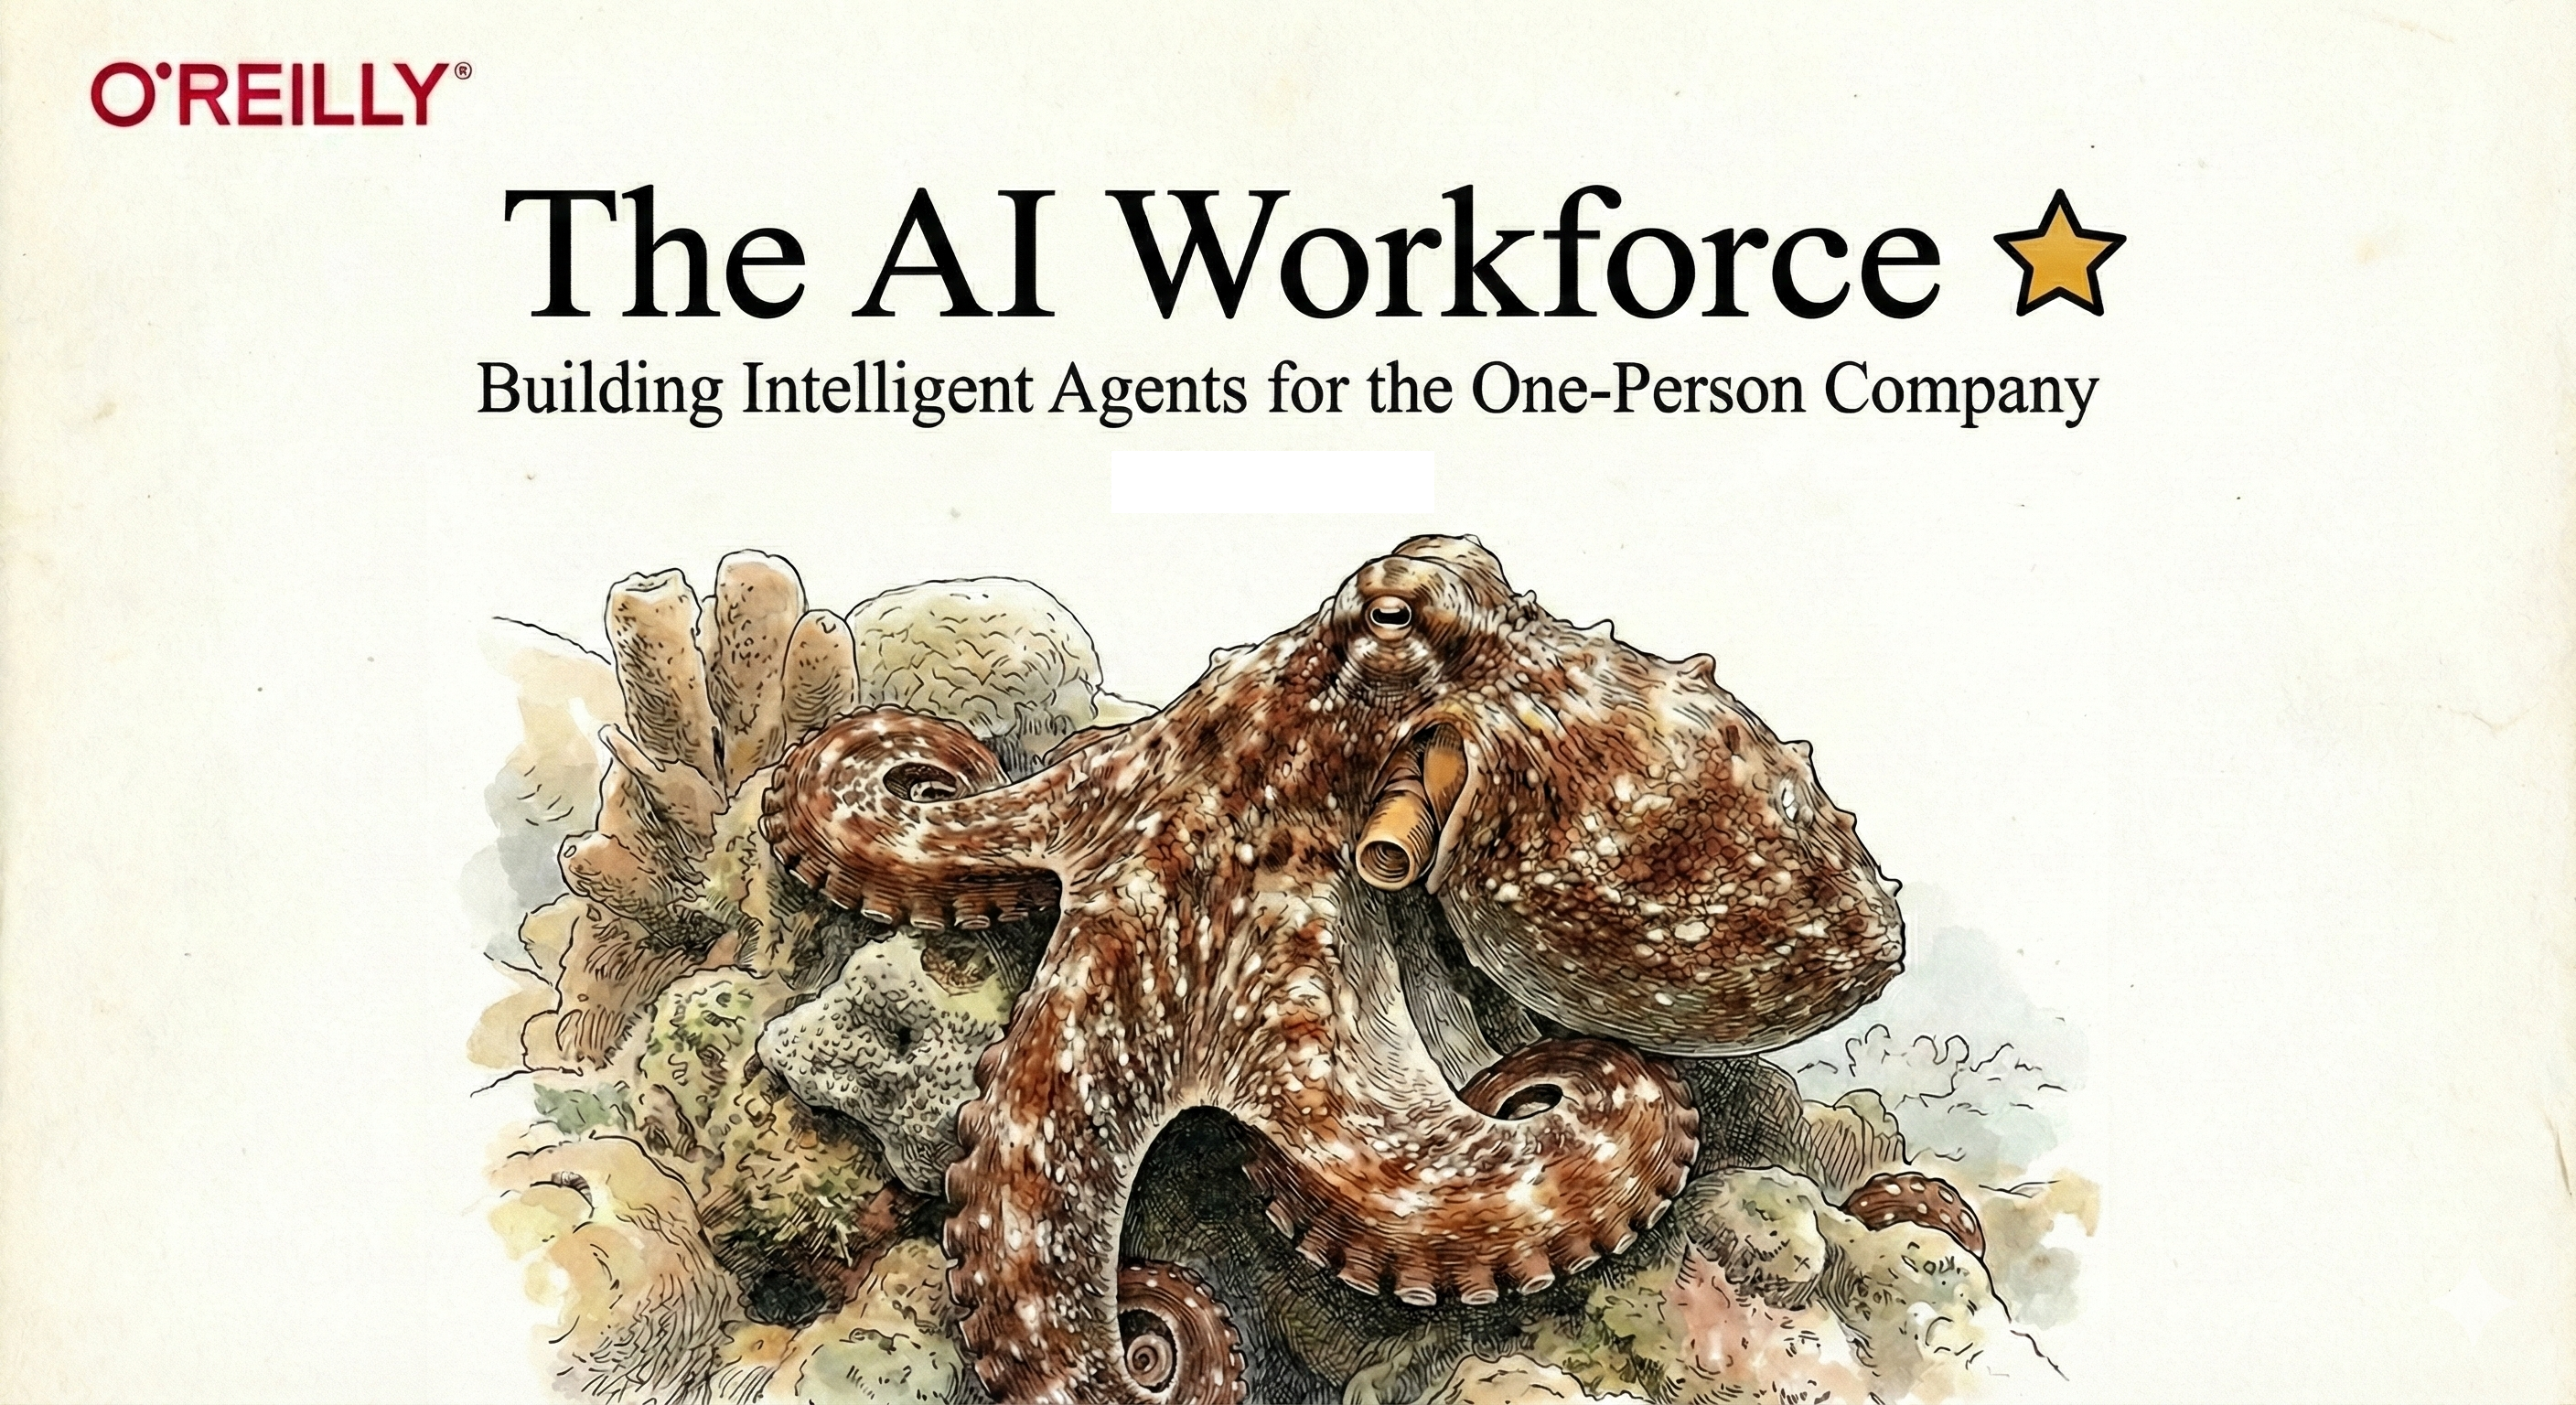
\includegraphics[width=3in]{../images/cover-animal.png}

\vspace{1.2in}

{\Large Jim Xiao}

\vfill

{\large\color{oreilly-red}\textbf{O'REILLY}}
\end{center}
\newpage

%% COPYRIGHT
\thispagestyle{empty}
\vspace*{\fill}
\begin{small}
\noindent\textbf{The AI-Powered One-Person Company}\\
\textit{From Solopreneur to Scale: Building Your AI Agent Workforce}\\
by Jim Xiao

\vspace{1.5em}
\noindent Copyright \textcopyright\ 2026 Jim Xiao. All rights reserved.

\vspace{1em}
\noindent Printed in the United States of America.

\vspace{1em}
\noindent Published by O'Reilly Media, Inc., 1005 Gravenstein Highway North, Sebastopol, CA 95472.

\vspace{1em}
\noindent O'Reilly books may be purchased for educational, business, or sales promotional use. Online editions are also available for most titles (\textit{https://oreilly.com}). For more information, contact our corporate/institutional sales department: 800-998-9938 or \textit{corporate@oreilly.com}.

\vspace{1em}
\noindent\textbf{Acquisitions Editor:} TBD\\
\textbf{Development Editor:} TBD\\
\textbf{Production Editor:} TBD\\
\textbf{Copyeditor:} TBD\\
\textbf{Proofreader:} TBD\\
\textbf{Indexer:} TBD\\
\textbf{Interior Designer:} TBD\\
\textbf{Cover Designer:} TBD\\
\textbf{Illustrator:} TBD

\vspace{1em}
\noindent January 2026: First Edition

\vspace{1em}
\noindent\textbf{Revision History for the First Edition}\\
2026-01-15: First Release

\vspace{1em}
\noindent See \textit{https://oreilly.com/catalog/errata.csp?isbn=9781234567890} for release details.

\vspace{1em}
\noindent The O'Reilly logo is a registered trademark of O'Reilly Media, Inc. \textit{The AI-Powered One-Person Company}, the cover image, and related trade dress are trademarks of O'Reilly Media, Inc.

\vspace{1em}
\noindent The views expressed in this work are those of the author and do not represent the publisher's views. While the publisher and the author have used good faith efforts to ensure that the information and instructions contained in this work are accurate, the publisher and the author disclaim all responsibility for errors or omissions, including without limitation responsibility for damages resulting from the use of or reliance on this work. Use of the information and instructions contained in this work is at your own risk.

\vspace{1em}
\noindent 978-1-234-56789-0\\
{[}LSI{]}
\end{small}
\newpage

%% DEDICATION
\thispagestyle{empty}
\vspace*{2.5in}
\begin{center}
\textit{\large For every entrepreneur who dared to build alone,\\[0.5em]
and for the AI partners who now stand beside them.}

\vspace{2em}

\textit{And to my family,\\[0.3em]
who believed in this vision before anyone else could see it.}
\end{center}
\newpage

%% ============================================================
%% PREFACE
%% ============================================================
\chapter*{Preface}
\addcontentsline{toc}{chapter}{Preface}

\begin{center}
\begin{tikzpicture}[scale=0.8]
    % AI Agent illustration
    \draw[thick, oreilly-red, fill=oreilly-red!10] (0,0) circle (1.5cm);
    \node at (0,0) {\Large\textbf{AI}};

    % Surrounding agents
    \foreach \angle/\name in {60/Emma, 120/Sam, 180/Maya, 240/Casey, 300/Finn, 0/Oscar} {
        \draw[thick, oreilly-gray] (\angle:2.5cm) circle (0.8cm);
        \node[font=\small] at (\angle:2.5cm) {\name};
        \draw[->, thick, oreilly-red!60] (\angle:1.6cm) -- (\angle:1.7cm);
    }

    % Central connection
    \node[below] at (0,-3.5) {\textit{Your AI Agent Team}};
\end{tikzpicture}
\end{center}

\vspace{1em}

When I first started writing this book, I asked myself a simple question: if I could tell my past self everything I've learned about AI and business over the past three years, what would I say?

The answer is the book you're holding.

\vspace{0.5em}

In 2023, I was like most entrepreneurs: overwhelmed by daily operations, working sixty to seventy hours a week, and feeling like I was always catching up. I knew AI was changing the world, but I didn't know how it could change \textit{my} world.

\vspace{0.5em}

Three years later, my business runs on six AI agents. I work thirty hours a week. My revenue has doubled. More importantly, I've rediscovered the original purpose of entrepreneurship---doing meaningful work, not being drowned by it.

\vspace{0.5em}

This book isn't about the future of AI. It's about the \textbf{present}---the concrete systems, proven methods, and practical tools you can implement today.

\vspace{0.5em}

Welcome to the new era of the one-person company.

\vspace{2em}
\begin{flushright}
\textit{Jim Xiao}\\
\textit{January 2026}
\end{flushright}

\newpage

%% ============================================================
%% INTRODUCTION: HOW TO USE THIS BOOK
%% ============================================================
\chapter*{Introduction: How to Use This Book}
\addcontentsline{toc}{chapter}{Introduction: How to Use This Book}

\section*{Book Structure}

This book is divided into eight parts, designed to be read cover-to-cover or used as a reference manual:

\begin{center}
\begin{tikzpicture}[
    node distance=0.7cm,
    box/.style={rectangle, draw=oreilly-red, fill=oreilly-red!10, text width=5.5cm, minimum height=0.9cm, align=center, rounded corners=3pt, font=\small},
    arrow/.style={->, thick, oreilly-gray}
]
    \node[box] (p1) {Part I: The Paradigm Shift\\(Chapters 1--3)};
    \node[box, below=of p1] (p2) {Part II: Your AI Agent Team\\(Chapters 4--9)};
    \node[box, below=of p2] (p3) {Part III: The AI-Native Business\\(Chapters 10--11)};
    \node[box, below=of p3] (p4) {Part IV: Technical Infrastructure\\(Chapters 12--14)};
    \node[box, below=of p4] (p5) {Parts V--VII: Playbooks \& Transformation\\(Chapters 15--18)};
    \node[box, below=of p5] (p6) {Part VIII: The Next Frontier\\(Chapters 19--21)};

    \draw[arrow] (p1) -- (p2);
    \draw[arrow] (p2) -- (p3);
    \draw[arrow] (p3) -- (p4);
    \draw[arrow] (p4) -- (p5);
    \draw[arrow] (p5) -- (p6);
\end{tikzpicture}
\end{center}

\section*{Reading Recommendations}

\begin{itemize}
\item \textbf{Beginners:} Start from the beginning and read sequentially. Each chapter builds on the previous one.
\item \textbf{Eager implementers:} Read Chapter 1 for the big picture, then skip to Chapter 18's 90-day plan, and come back to fill in the details.
\item \textbf{Technical readers:} You can jump directly to Part IV (Technical Infrastructure), but we recommend skimming Chapter 2 first to understand the design philosophy.
\item \textbf{Specific needs:} Each agent chapter (Chapters 4--9) is self-contained and can be read and implemented independently.
\end{itemize}

\section*{Conventions Used in This Book}

\begin{note}[Note]
Boxes like this contain supplementary information, background knowledge, or additional explanations.
\end{note}

\begin{tip}[Tip]
Tip boxes contain practical advice and best practices.
\end{tip}

\begin{warning}[Warning]
Warning boxes identify common pitfalls and mistakes to avoid.
\end{warning}

\begin{keyinsight}[Key Insight]
Key insight boxes summarize the main takeaways from each chapter or section.
\end{keyinsight}

\newpage

%% TABLE OF CONTENTS
\tableofcontents
\newpage

%% ============================================================
%% PART 1: THE PARADIGM SHIFT
%% ============================================================
\part{The Paradigm Shift}

\chapter{一人公司革命}\index{一人公司}

\section{自由的承诺}

让我告诉你一切改变的那个时刻。

那是一个周二晚上11点。我坐在家庭办公室里,被又一个14小时工作日的残骸包围:

\begin{itemize}
\item 我的收件箱显示47封未读邮件
\item 我的Slack有23条未读消息
\item 一份客户提案半完成地躺在屏幕上,明天就要交
\item 在这周的混乱中,我忘记了发送一张价值8000美元的发票——那是两周前完成的工作
\end{itemize}

我赚得不少——年收入超过30万美元——但我也在慢慢死去。不是戏剧性地,不是突然地,而是缓慢地。本应给我自由的生意变成了我的牢笼。我是一切的瓶颈。没有什么事情会发生,除非我亲自做、亲自审核、亲自批准或亲自修复。

\textbf{听起来熟悉吗?}

如果你拿起这本书,你现在可能正在点头。你可能正在经营一家咨询公司、一家电商店铺、一个SaaS产品或一家服务机构。你擅长你所做的事情。你建立了真实的东西。但你也被自己的成功所困。

这就是我想让你明白的:\textbf{不必如此。}

在过去的十八个月里,我用AI智能体从头重建了我的业务。不是科幻小说里的那种——不是某个为我做决定的自主机器人。我说的是实用的、可实施的AI系统,它们处理我业务中可预测的部分,而我专注于真正重要的工作。

结果?我每周工作30小时而不是70小时。我的收入翻了一番。我的压力大幅下降。自从我创业以来,我第一次真正度假而不检查邮件。

这本书是我希望在开始这次转型时就拥有的指南。我学到的一切,我犯的每一个错误,我建立的每一个系统——都在这里。当你读完时,你将拥有一个具体的计划来建立你自己的AI赋能一人公司。

让我们开始吧。

\section{为什么这一刻与众不同}

每隔几年,某位技术专家就会宣布一场「革命」。云计算本应改变一切。移动互联网本应改变一切。第一波聊天机器人本应改变一切。

这些革命大多被证明是渐进式改进。有用,是的。革命性,不是。

那么,为什么你应该相信AI智能体有什么不同?

\textbf{2025-2026年有三件事汇聚在一起,使这一刻真正与众不同:}

\subsection{经济终于可行了}

2023年,运行一个有用的AI助手每月需要数百美元的API费用,而且质量不稳定,你花在修正输出上的时间和自己做这项工作的时间一样多。

2026年,每月20美元订阅Claude Pro或ChatGPT Plus,你就能获得两年前需要5万美元定制软件开发的AI能力。成本暴跌的同时质量飙升。

让我具体说明。我的AI智能体「Emma」处理邮件分类、日程安排和常规通信。她每天为我处理大约50封邮件。成本?大约每天2美元的API使用费。每月60美元,我拥有了以前需要每月1500美元虚拟助理才能提供的服务——除了Emma永不睡觉,永不请病假,永不打错字。

\subsection{学习曲线崩塌了}

你不需要编程。你不需要理解机器学习。你不需要计算机科学学位。

你需要清晰地写作。就这样。

如果你能向一个聪明的新员工解释你想如何完成某事,你就能训练一个AI智能体。驱动我业务的提示是用简单的英语写的。它们看起来像这样:

\begin{quote}
「当新邮件到达时,检查发件人是否在我们的客户列表中。如果是,优先处理并起草一个热情的回复。如果不是,分类为潜在客户、供应商或其他。对于潜在客户,根据我们的标准进行资格审查并起草适当的回复。标记任何涉及金钱、法律事务或不满意客户的邮件供我亲自审阅。」
\end{quote}

那不是代码。那只是清晰的思考写下来。如果你能做到这一点,你就能构建AI智能体。

\subsection{质量跨越了门槛}

输出现在足够好用于专业用途。

我不是说AI写得和你最好状态下的最佳作品一样好。它做不到。但它写得和你周五下午4点疲惫时的作品一样好——那正是你大多数常规通信被写出的时候。

对于客户支持邮件,AI草稿在大约85\%的情况下与人类写的回复无法区分。对于初次潜在客户回复,它们实际上\textit{比}大多数人写的更好,因为它们一致、及时,而且永不烦躁。

剩下的15\%?那些会被标记供人工审阅。AI知道它不知道什么,这比我共事过的一些人还强。

\section{一人公司愿景}

OpenAI首席执行官Sam Altman做了一个在商界引起轰动的预测:\textit{「我们可能很快会看到第一家十亿美元的一人公司。」}

一个人运营的十亿美元公司。想想这意味着什么。

现在,我不指望你建立一家十亿美元的公司,坦率地说,我也不打算这样做。但这就是为什么Altman的预测很重要:

\begin{itemize}
\item 如果一个人理论上可以用AI建立一家十亿美元的公司,那么一个人绝对可以建立一家百万美元的公司
\item 或者一家50万美元的公司
\item 或者任何规模的公司,只要能给你想要的自由、收入和影响力
\end{itemize}

个体创业者规模的约束一直是时间。一天只有这么多小时,当每一小时的收入都需要一小时的工作时,你很快就会触及天花板。

\textbf{AI智能体打破了这个约束。}

让我向你介绍现在运营我业务的团队:

\textbf{Emma}是我的行政助理。她处理邮件分类、日程安排和常规通信。在我每天早上看到收件箱之前,Emma已经对所有内容进行了分类,为常规项目起草了回复,并标记了3-5件真正需要我关注的事情。她每天为我节省2-3小时。

\textbf{Sam}是我的销售开发代表。当潜在客户进来时——从我的网站、推荐或其他任何地方——Sam根据我的标准对他们进行资格审查,研究他们的公司,并起草个性化的回复。从潜在客户到达到首次联系的平均时间过去是24-48小时(每当我有空的时候)。现在不到5分钟。

\textbf{Maya}是我的营销经理。她创建内容、管理社交媒体并处理营销活动。她起草我的每周通讯,创建社交帖子,并在各平台上重新利用我的想法。过去需要我每周8-10小时的工作现在只需要2小时的审阅和润色。

\textbf{Casey}是我的客户成功经理。她处理支持咨询、接待新客户,并关注客户健康指标。客户获得比我独自能提供的更快、更一致的支持。

\textbf{Finn}是我的财务智能体。他生成发票、发送付款提醒,并准备财务摘要。六个月来我没有手动追讨过一笔逾期付款。

\textbf{Oscar}是我的运营智能体。他协调履行、管理供应商通信,并在幕后保持业务顺利运行。

加在一起,这个团队每月花费我大约500美元的AI工具和API使用费。等效的人类团队每月将花费15000-20000美元。这个数学不微妙。

\section{两个周一的故事}

让我向你展示这在实践中是什么样子。

\subsection{没有AI智能体的周一}

你的闹钟在早上6:30响起。你的第一个想法,在你睁开眼睛之前,是关于你昨天没有回复的邮件。焦虑已经在那里了,胃里熟悉的结。

到7:00,你端着咖啡坐在桌前,盯着有47封新消息的收件箱。你开始分类。删除。删除。转发到以后。这封需要回复——但你需要先查找项目细节。标记它。这封很紧急——一个客户对某事不满。你的心率飙升。立即回复,可能太快了,可能不是你最好的作品。

到8:30,你可能处理了15封邮件。你回复了5封。紧急的客户问题部分解决了,但你被打乱了。

上午9:00有一个销售电话。你应该了解这个潜在客户,但你什么时候有时间研究他们?你即兴发挥。还行,不算好。

上午10:00到中午12:00应该用来写那份你需要完成的提案。但你的手机一直在响。Slack一直在叮。有人有一个「快速问题」变成了30分钟的离题。到中午,你写了两段。

午餐是在桌前吃的,同时你试图赶上邮件。

下午1:00是一个客户电话,因为没有提前准备任何东西而拖得很长。

下午2:30你想起你上周应该发送的那张发票。你花30分钟创建它,然后意识到你需要三周笔记中的信息。发票终于在下午3:45发出。它应该在十天前就发出了。

下午4:00你再次尝试写提案。你取得了进展,但你累了,质量可以看出来。

下午6:00你离开,感到挫败。提案还没完成。你今晚晚饭后会完成它,这意味着你不会真正陪伴家人。又一次。

晚上9:00你发送提案,希望它足够好。

晚上11:00你「再检查一次」邮件,发现三个新的火灾,明天会从今天结束的地方开始。

总工作时间:14+小时。战略进展:零。剩余精力:负数。

\subsection{有AI智能体的周一}

你的闹钟在早上7:00响起。你睡得很好,因为你睡前没有检查邮件——Emma处理夜间分类。

你和家人一起吃早餐。真正的早餐,坐下来,在场。

到8:00,你在桌前。你打开你的指挥中心——一个简单的仪表板,显示你的智能体一夜之间做了什么。Emma处理了47封邮件:

\begin{itemize}
\item 38封被自动处理(常规回复、日程安排、供应商协调)
\item 6封等待你的审阅(草稿已准备好)
\item 3封被标记为重要(附有摘要)
\end{itemize}

你花15分钟审阅Emma的草稿。五封完美;你点击发送。一封需要为VIP客户添加个人风格;你添加两句话然后发送。

三个标记的项目包括那个不满的客户。但Emma已经收集了上下文:客户的历史、问题细节和建议的解决方案。你在10分钟而不是45分钟内写了一个深思熟虑的回复。

到8:30,你的收件箱清空了。不是收件箱为零的表演艺术——真正清空了。一切要么被处理,要么被委托给智能体,要么被安排到以后。

上午9:00有那个销售电话。但这次,Sam准备了一份简报:潜在客户的公司背景、最近的新闻、潜在痛点和建议的谈话要点。电话进行得很好。你成交了。

上午10:00到中午12:00是提案时间。你的手机设置为勿扰。你的智能体处理来信。你在一种你已经忘记的心流状态中写作。提案在11:30完成。

午餐就是午餐。

下午1:00客户电话。Casey准备了议程和相关背景。你专注而高效。

下午2:00你有了一个新服务的想法。你花一个小时勾画它,几周来第一次战略性地思考业务。

下午3:00你审阅Maya本周的内容日历。看起来不错。你批准了它。

下午3:30你检查智能体仪表板。一切运行顺利。你处理两个需要人类判断的快速决定。

下午4:00你意识到没有什么紧急的事情了。这是一种陌生的感觉。

下午4:30你去散步。

下午5:15你处理几件小事然后收工。

总工作时间:8小时。战略进展:显著。剩余精力:正数。

这不是幻想。这是我现在真实的周一。它也可以是你的。

\section{解放的经济学}

让我们谈谈钱,因为数字很重要。

\subsection{人工帮助的成本}

如果你想雇用相当于我的AI智能体团队的人类——即使是兼职,即使是海外——你将面对的是:

\begin{itemize}
\item 行政助理(兼职):每月1500美元
\item 销售开发代表(兼职):每月3000美元
\item 营销经理(兼职):每月2000美元
\item 客户支持(兼职):每月2000美元
\item 簿记员:每月800美元
\item 运营协调员(兼职):每月1500美元
\end{itemize}

总计:每月10800美元,或每年约13万美元。

这还是兼职帮助。当你考虑以下因素时,实际成本更高:

\begin{itemize}
\item 管理开销(你管理他们的时间)
\item 培训时间(以及他们离开时的再培训)
\item 跨时区异步通信的延迟
\item 需要你干预的不可避免的错误
\end{itemize}

大多数个体创业者负担不起每年13万美元的员工费用。所以相反,他们自己做所有事情然后倦怠。

\subsection{AI智能体的成本}

这是我实际的AI智能体支出:

\begin{itemize}
\item Claude Pro订阅:每月20美元
\item 额外API使用:每月100-200美元
\item 自动化平台(n8n/Make):每月50美元
\item 相关工具和集成:每月100美元
\end{itemize}

总计:每月300-400美元,或每年约4500美元。

\begin{figure}[H]
\centering
\begin{tikzpicture}[scale=0.9]
    % Draw bars
    \fill[oreilly-gray!30] (0,0) rectangle (2,6.5);
    \fill[oreilly-red!70] (3,0) rectangle (5,0.225);

    % Labels
    \node[below] at (1,0) {\small 人力团队};
    \node[below] at (4,0) {\small AI智能体};

    % Values
    \node[above] at (1,6.5) {\textbf{\$13万/年}};
    \node[above] at (4,0.225) {\textbf{\$0.45万/年}};

    % Y-axis
    \draw[->] (-0.5,0) -- (-0.5,7) node[above, rotate=90, anchor=south] {\small 年度成本};
    \foreach \y/\label in {0/\$0, 3.25/\$6.5万, 6.5/\$13万} {
        \draw (-0.6,\y) -- (-0.4,\y);
        \node[left] at (-0.6,\y) {\tiny \label};
    }

    % Annotation
    \draw[<->, thick, oreilly-red] (5.5,0.225) -- (5.5,6.5);
    \node[right, align=left] at (5.7,3.3) {\small \textbf{96\%}\\\small 节省};
\end{tikzpicture}
\caption{年度成本对比:人力团队 vs AI智能体}
\label{fig:cost-comparison-cn}
\end{figure}

这是96\%的成本降低\index{成本降低},而能力在很多方面是优越的。我的AI智能体全天候工作。它们永远不会有糟糕的一天。它们永远不会不通知就辞职。它们对困难的客户有无限的耐心。

\subsection{真正的投资回报率}

但成本节省甚至不是主要故事。真正的回报是在你的时间上。

假设你是一个每小时收费200美元的顾问(或经营一个你的时间每小时创造200美元价值的企业)。假设AI智能体每周为你节省30小时。

那是每周6000美元的时间价值被重新获得。每月24000美元。每年288000美元。

其中一些时间你会再投资于发展业务。其中一些你会用来真正拥有生活。无论哪种方式,你都在取回你拥有的最稀缺的资源:你一生中宝贵的时间。

当我这样框定时,问题不是你是否负担得起AI智能体。问题是你是否负担得起不使用它们。

\section{使之有效的四个原则}

在我们深入实施之前——我们会详细讨论——我想分享四个原则,它们区分了成功的AI智能体部署和昂贵的失败。

\subsection{原则1:上下文就是一切}

这是大多数人搞错的地方:他们认为AI是一个魔法盒子,你把任务扔进去就能得到结果。

这对简单的、一次性的请求有效。对于业务运营来说,它完全失败。

通用AI和有用的AI助手之间的区别是\textit{上下文}。你的AI需要知道你的客户是谁,你承诺了他们什么,你的声音是什么样的,以及你喜欢如何处理情况。没有上下文,你会得到需要不断纠正的通用输出。

实际含义:你需要一个知识库。不是一个花哨的数据库——只是包含你的AI需要知道的一切的Markdown文件:

\begin{itemize}
\item 包含历史和偏好的客户文件
\item 流程文档(我们如何做事)
\item 常见通信的模板
\item 你的品牌声音指南
\item 常见情况的决策标准
\end{itemize}

我们将在第2章构建这个,你将在整本书中使用它。它是其他一切所依赖的基础。

\subsection{原则2:专业化胜过通用化}

不要试图构建一个做所有事情的超级AI。构建具有明确职责的专业化智能体。

这就是为什么我有Emma、Sam、Maya、Casey、Finn和Oscar,而不是一个处理所有事情的超级智能体「Alex」。专业化的智能体:

\begin{itemize}
\item 有产生一致结果的聚焦提示
\item 不会对他们正在扮演的角色感到困惑
\item 可以独立改进
\item 孤立失败而不是拖垮所有东西
\end{itemize}

当Emma处理邮件时,她在思考邮件。她不是在试图同时记住销售手册和客户支持协议。这种清晰度使她更加有效。

\subsection{原则3:编排,而非自动化}

编排和自动化之间有一个关键区别。

自动化是:「当X发生时,做Y。」

编排是:「当X发生时,分析情况,考虑相关上下文,决定什么样的响应是适当的,然后根据信心水平处理它或升级它。」

老式自动化(Zapier触发器、基本工作流)不断崩溃,因为世界不适合整洁的IF-THEN规则。AI编排优雅地处理模糊性。它可以说,「这看起来像一个销售咨询,但语气表明这个人可能对某事不满。让我起草一个承认两种可能性的回复。」

你的AI智能体不只是执行;它们思考(在它们的专业领域内)。

\subsection{原则4:信任是赢得的,不是假设的}

这是大多数人忽略的原则,也是为什么大多数AI实施失败的原因。

模式总是一样的:有人对AI感到兴奋,部署了一个自主权太大的智能体,智能体犯了一个损害客户关系的错误,整个项目被放弃,认为「还没准备好投入生产」。

解决方案是逐步建立信任:

\textbf{第1-4周:仅草稿。}AI提议行动;你批准每一个。这不是低效——这是培训。你在教AI你的偏好,同时建立你对其能力的信心。

\textbf{第2-3个月:常规自主。}AI可以自主执行常规操作,但任何不寻常的事情仍然需要你的批准。

\textbf{第4个月以后:在训练模式上完全自主。}AI在它已经被训练的所有事情上独立运行。你做抽查而不是审阅所有内容。

这个进展通常需要90天。试图跳过几乎总是以糟糕的方式结束。

\section{这本书适合谁(不适合谁)}

我想诚实地说明谁会从这本书中获得价值。

\subsection{如果你...这本书适合你}

你是一个个体创业者或运营一个小团队(1-5人),而且你有真正的收入。不是副业——一个真正支付你账单并且还有剩余的业务。

你擅长你所做的事情。你有重视你工作的客户。问题不是你的业务不运作;问题是它运作得\textit{太好}而你跟不上。

你被运营工作淹没。邮件、日程安排、开发票、支持、内容——保持灯亮着的必要但令人疲惫的工作。你知道你应该做更多战略工作,但永远没有时间。

你对技术感到舒适。不一定是开发人员,但可以在没有大量指导的情况下弄清楚新工具。如果你能在一个下午学会使用一个新应用程序,你就有足够的技术能力做这件事。

你对迭代有耐心。这不是一个「设置后就忘记」的系统。部署需要2-3个月,并且需要持续改进。回报是巨大的,但不是即时的。

\subsection{如果你...这本书不适合你}

你是一个寻找部署指南的企业IT团队。这是一本为运营者而写的书,不是基础设施架构师。

你是一个想从头构建AI智能体的开发人员。我们使用现有工具,而不是构建自定义模型。如果你想深入技术实现,有更好的资源。

你在一个高度监管的行业(医疗保健、金融服务、法律)并且需要合规指导。这本书会向你展示什么是可能的,但在实施之前你需要专业的合规专业知识。

你在寻找快速致富计划。建立一个AI赋能的企业是真正的工作。它比替代方案的工作量少,但仍然是工作。如果你对努力过敏,这不会帮助你。

\section{你将构建什么}

当你读完这本书时,你将拥有:

\textbf{一个完整的AI智能体团队},为你的业务量身定制——Emma、Sam、Maya、Casey、Finn和Oscar(或你给它们起的任何名字),每个都处理你运营的特定领域。

\textbf{一个统一的知识库},使你的AI智能体真正理解你的业务、你的客户和你的偏好。

\textbf{与你现有工具的集成}——你的邮件、日历、CRM和你使用的任何其他东西——所以你的AI智能体在你当前的工作流程中工作,而不是要求你改变一切。

\textbf{一个监控系统},让你看到你的智能体在做什么,在问题变成问题之前发现它们,并持续改进它们的性能。

\textbf{一个可持续的运营节奏},你每天花5-6小时做实际工作,而不是12-14小时处理混乱。

最重要的是,你将取回你的生活。

\section{前方的道路}

这本书的其余部分是这样展开的:

\textbf{第一部分(第1-3章)}建立范式转变:AI智能体是什么,它们如何融入你的业务,以及2026年可用的工具景观。

\textbf{第二部分(第4-9章)}介绍你的AI智能体团队。每一章深入介绍一个智能体:它们的能力,如何设置它们,真实的提示和模板,以及需要注意的常见问题。

\textbf{第三部分(第10-11章)}涵盖AI原生业务基础设施:如何构建你的知识库,为什么「文件夹结构作为操作程序」是关键洞见,以及如何构建AI原生CRM。

\textbf{第四部分(第12-14章)}深入技术:构建你的智能体栈,编写有效的提示和手册,以及监控/调试/改进你的系统。

\textbf{第五部分(第15-16章)}提供销售自动化和营销系统的进阶手册。

\textbf{第六部分(第17章)}讲述一个完整转型的故事,从不堪重负的运营者到AI增强的企业主。

\textbf{第七部分(第18章)}给你90天行动计划:每周要做什么,以实施这本书中的所有内容。

\textbf{第八部分(第19-21章)}探索下一个前沿:AI作为专业专家(律师、医生、会计师)、Claude OS的MCP应用革命,以及如何用Obsidian构建你的AI原生第二大脑。

前方的旅程是实用的、详细的、可操作的。没有空话。没有填充物。只有我建立的系统,我学到的教训,以及你需要建立自己的AI赋能一人公司的蓝图。

让我们开始吧。

\section{章节总结}

你在这章学到的内容:

\begin{enumerate}
\item AI智能体革命是真实的,正在发生。经济可行,学习曲线可接近,质量已经可以投入生产。

\item 一个专业化AI智能体团队(Emma、Sam、Maya、Casey、Finn、Oscar)可以以每月不到500美元的价格替代相当于每月15000美元以上的人工帮助。

\item 真正的价值不仅仅是成本节省——而是时间解放。每周取回30+小时改变了你的业务运营方式和你的生活方式的一切。

\item 四个原则支配成功的实施:上下文就是一切,专业化胜过通用化,编排胜过自动化,信任是赢得的而不是假设的。

\item 这本书将给你一个完整的、可实施的系统——但它需要耐心、迭代和90天的持续努力。
\end{enumerate}

\textbf{下一章:}我们将探索「AI即操作系统」——从数据库驱动业务到知识图运营的范式转变,以及为什么你的文件夹结构成为你的标准操作程序。

\chapter{AI as Operating System - The New Business Methodology}

\section{The Discovery That Changed Everything}

I spent three months trying to teach my AI assistant how to handle customer emails. Every morning, I'd review its work, find mistakes, explain what went wrong, and hope it would do better tomorrow. It never did:

\begin{itemize}
\item The responses were technically correct but felt robotic
\item It missed context
\item It didn't understand our customers
\end{itemize}

Then I discovered something that changed everything: \textbf{I was teaching the wrong way.}

I was treating the AI like a new employee---giving verbal instructions, hoping it would learn from experience, getting frustrated when it didn't remember our conversation from last week. But AI agents don't work like humans:

\begin{itemize}
\item They don't accumulate wisdom from experience
\item They don't ``pick things up'' over time
\item What they do brilliantly is follow documented processes---precisely, consistently, at any hour of the day
\end{itemize}

\textbf{The moment I stopped training and started documenting, everything changed.}

\section{Your Business as an Operating System}

Think about your computer's operating system. When you click a file, the OS doesn't ``figure out'' what to do---it follows precise instructions coded by engineers. When you print a document, it executes a defined process. The OS is essentially a massive collection of documented procedures.

\textbf{Your business can work the same way.}

For decades, we've treated business knowledge as something that lives in people's heads:

\begin{itemize}
\item The veteran salesperson ``just knows'' how to handle objections
\item The experienced customer service rep ``has a feel'' for when to escalate
\item The CEO ``instinctively'' prioritizes emails
\end{itemize}

This tacit knowledge is valuable. It's also fragile, inconsistent, and doesn't scale.

The AI-native business inverts this model. Instead of keeping knowledge in heads and hoping people execute it correctly, you document everything in files and let AI agents execute it perfectly.

Here's what that looks like:

\begin{itemize}
\item \textbf{Your folder structure becomes your organizational chart.} Sales, Marketing, Customer Success, Finance---each department is a folder.
\item \textbf{Markdown files become employee training.} Every playbook, every procedure, every decision tree---documented and executable.
\item \textbf{AI agents become your workforce.} Each one reads its assigned playbooks and executes accordingly.
\item \textbf{You become the strategist.} Not the doer, but the architect of how things get done.
\end{itemize}

\section{The Consultant's Secret}

I learned this lesson from an unlikely source: management consultants.

Have you ever wondered how McKinsey can deploy a 22-year-old fresh from business school to advise Fortune 500 CEOs? It's not because they hire geniuses. \textbf{It's because they have frameworks.}

A McKinsey consultant doesn't solve problems from scratch. They apply documented methodologies:

\begin{itemize}
\item The 7-S Framework for organizational analysis
\item The Three Horizons for growth strategy
\item The MECE principle for problem decomposition
\end{itemize}

These frameworks are written down. They're taught. They're reusable.

When a consultant leaves the firm, the frameworks stay behind. When a new consultant joins, they learn from the documentation, not just from shadowing senior colleagues.

\textbf{This is exactly how your AI-powered business should work.}

Your business toolkit mirrors theirs:

\begin{itemize}
\item \textbf{Frameworks} tell you how to think about problems. In your business, these become the ``README'' files in each department folder.
\item \textbf{Playbooks} provide step-by-step procedures. These are your markdown files---detailed enough that anyone (or any AI) could follow them.
\item \textbf{Templates} ensure consistent outputs. These live in templates folders, ready to be customized.
\item \textbf{Checklists} maintain quality. Embedded in your playbooks as verification steps.
\end{itemize}

The key insight is simple: If a new consultant can read your playbook and execute it correctly, so can an AI agent.

\section{Building Your Knowledge Architecture}

When I redesigned my business around this principle, I created a folder structure that still guides my operations today. Let me walk you through it---not as a template to copy blindly, but as a thinking framework you can adapt.

The root of my business lives in a folder called \texttt{/company}. Inside, I have departments: sales, marketing, customer-success, finance, operations, and executive. Each department follows the same internal structure:

\begin{codebox}
\begin{lstlisting}[style=python]
/department
|-- /playbooks        (how we do things)
|-- /templates        (what we produce)
|-- /agents           (who does the work)
`-- README.md         (department overview)
\end{lstlisting}
\end{codebox}

The playbooks folder is where the magic happens. Take my sales department. Inside \texttt{/sales/playbooks}, I have:

\begin{itemize}
\item \texttt{lead-qualification.md} --- How we decide if a lead is worth pursuing
\item \texttt{cold-outreach.md} --- How we approach prospects who don't know us
\item \texttt{objection-handling.md} --- How we respond to common pushbacks
\item \texttt{demo-process.md} --- How we run product demonstrations
\item \texttt{closing-sequence.md} --- How we move from proposal to signed contract
\end{itemize}

Each file is detailed enough that a complete stranger---or an AI agent---could execute the process correctly on their first attempt.

\section{What Makes Markdown Magical}

You might wonder: why markdown? Why not a database, a wiki, or specialized business software?

Markdown hits a rare sweet spot. It's human-readable---you can write and edit it in any text editor. It's AI-readable---language models parse markdown naturally, understanding headers, lists, and links. It's version-controlled---every change tracked in Git, creating a complete history of how your business evolved. And it's platform-agnostic---you're not locked into any vendor's ecosystem.

But the most important reason is portability. When I show my playbooks to an AI agent, I can include them in a prompt, attach them to a context window, or have the agent read them from a file. No API integrations. No special formatting. Just text.

Here's what a real playbook looks like in my system:

\begin{codebox}
\begin{lstlisting}[style=bash]
# Lead Qualification Playbook

## Objective
Identify leads worth pursuing within 5 minutes of inquiry.

## Qualification Criteria (BANT)

### Budget
The lead signals financial capacity:
- Company has > 10 employees OR
- They mentioned a specific budget OR
- Their industry typically pays our price point

### Authority
The person can make or influence the decision:
- Title includes: Founder, CEO, VP, Director, Head of
- They're the decision maker mentioned in the inquiry
- They were referred by an existing customer

### Need
They have a real problem we solve:
- They mentioned a specific pain point
- They indicated a timeline
- They're currently using a competitor

### Timeline
They're ready to act:
- Looking to implement within 90 days
- Mentioned urgency or a deadline
- Active evaluation in progress

## Scoring and Response

| Score | Classification | Response |
|-------|---------------|----------|
| 4/4   | HOT           | Respond in 1 hour, book meeting |
| 3/4   | WARM          | Respond in 4 hours, qualify more |
| 2/4   | NURTURE       | Add to email sequence |
| 1/4   | COLD          | Polite decline or long-term nurture |

## Escalation Rules
- Enterprise leads (>500 employees): Escalate to founder
- Competitor mentions: Use competitive positioning template
- Custom requirements: Schedule discovery call
\end{lstlisting}
\end{codebox}

When my sales agent, Sam, receives a new lead, he reads this playbook. He doesn't need to guess. He doesn't need to remember training from three months ago. The playbook tells him exactly what to do.

\section{The Power of Connected Knowledge}

Here's where the system becomes more powerful than the sum of its parts.

In tools like Obsidian, you can link notes to each other using double brackets: \texttt{[[another-note]]}. When you click the link, you jump to that note. This creates a web of interconnected knowledge---a knowledge graph.

Your business playbooks can work the same way.

Consider this customer onboarding document:

\begin{codebox}
\begin{lstlisting}[style=bash]
# Customer Onboarding

## Pre-Onboarding
Before the customer's start date:
- Run [[customer-health-check]]
- Review [[sales-notes]] from the deal

## Week 1
Get them to their first success:
- Send [[welcome-sequence]]
- Schedule [[kickoff-call]]
- Share [[getting-started-guide]]

## Week 2-4
Build the habit:
- Monitor [[health-score]]
- Follow [[check-in-cadence]]
- Document everything in [[customer-success-notes]]

## Related Processes
- [[renewal-process]] - 60 days before contract ends
- [[upsell-playbook]] - when ready for expansion
- [[escalation-matrix]] - when things go wrong
\end{lstlisting}
\end{codebox}

Every bracketed term is a link to another document. The onboarding playbook doesn't need to explain how to run a health check---it points to that playbook. This has three major benefits.

First, single source of truth. When you update \texttt{customer-health-check.md}, every playbook that references it gets the update automatically. No more hunting down every document that mentions the old process.

Second, progressive disclosure. The onboarding document stays clean and readable. Someone who wants the overview reads the main document. Someone who needs details clicks through to the linked playbooks.

Third, discoverability. By following links, an AI agent can explore your entire knowledge base. Ask it about onboarding, and it can trace the connections to health checks, success notes, and renewal processes.

\section{From Static Records to Living Context}

Traditional business tools store data in structured records. A CRM might have a contact entry like this:

\begin{codebox}
\begin{lstlisting}[style=python]
Name: John Smith
Email: john@company.com
Company: Acme Inc
Status: Prospect
Last Contact: 2026-01-15
\end{lstlisting}
\end{codebox}

This is accurate but lifeless. It tells you nothing about the relationship, the context, or what to do next.

In an AI-native system, the same contact becomes a rich context document:

\begin{codebox}
\begin{lstlisting}[style=bash]
# John Smith - Acme Inc

## Context
VP of Engineering at Acme Inc (50-200 employees).
Referred by [[Sarah Chen]] from [[XYZ Corp]].
Evaluating solutions for Q2 implementation.

## Conversation History

### 2026-01-15: Initial Call
John reached out after seeing our case study with Beta Corp.
His main pain point: current tool doesn't scale past 100 users.
Budget: $50-100K approved for this initiative.
Timeline: Needs decision by Feb 15 for Q2 implementation.
Also evaluating: [[Competitor A]] and [[Competitor B]].

### 2026-01-20: Demo
Impressed by our [[real-time-sync]] feature.
Concerned about [[legacy-system-integration]].
Next step: Technical review with his team next week.

## Relationship Map
- Reports to: CEO (final decision maker)
- Influenced by: CTO Sarah Jones (technical veto power)
- Knows: Mike at Beta Corp (our happy customer)

## Recommended Actions
1. Send [[case-study-beta-corp]] - similar company size
2. Schedule technical deep-dive for integration concerns
3. Ask Mike for a reference call with John
\end{lstlisting}
\end{codebox}

When your sales agent responds to John's email, it doesn't just know his name and company. It knows his pain points, his timeline, his concerns from the demo, and exactly what to do next.

\section{SOPs That Evolve}

Traditional Standard Operating Procedures share a common fate: they're written once, filed away, and slowly become obsolete while reality moves on.

I've seen the pattern repeatedly. Someone spends a week documenting processes. The documents go into a shared drive. Three months later, the actual process has changed, but the documentation hasn't. New employees learn from colleagues, not the SOP. The cycle continues.

AI-native SOPs break this pattern because they're actually used. Your AI agents read them before every action. If the SOP is wrong, the agent does the wrong thing. The immediate feedback forces you to keep documentation current.

But it goes further. Your AI agents can help the SOPs improve themselves.

Consider this email response playbook:

\begin{codebox}
\begin{lstlisting}[style=bash]
# Email Response Playbook
Last updated: 2026-01-28

## Subject Lines That Work
Based on last 30 days of data:
1. "Quick question about {{specific_topic}}" - 45% open rate
2. "Following up on {{previous_topic}}" - 38% open rate
3. "{{Mutual_connection}} suggested I reach out" - 52% open rate

## Subject Lines to Avoid
1. "Checking in" - 12% open rate
2. "Limited time offer" - 8% open rate

## Best Practices
- Respond within 5 minutes: 3x higher engagement
- Mention specific pain point: 2x higher reply rate
- Include clear next step: 4x higher conversion

## Current A/B Test
Testing formal vs. casual tone in initial responses.
Started: 2026-01-20
Results expected: 2026-02-03

## Update Log
- 2026-01-28: Updated subject line rankings (Maya)
- 2026-01-21: Added A/B test section (Maya)
- 2026-01-15: Initial version (Jim)
\end{lstlisting}
\end{codebox}

Maya, my marketing agent, updates this playbook automatically based on performance data. She tracks what works, retires what doesn't, and keeps the playbook current. The SOP isn't just a document---it's a living record of what actually works in my business.

\section{Making the Transition}

If this sounds overwhelming, take a breath. You don't need to document your entire business before starting. Here's how I approached it:

\textbf{Week 1: The Audit.} I listed everything I did repeatedly. Daily tasks: email, calendar, social media. Weekly tasks: invoicing, content creation, lead follow-up. Trigger-based tasks: responding to inquiries, handling support requests, processing orders.

\textbf{Week 2: The Structure.} I created my folder hierarchy. I didn't fill it with content yet---just the skeleton. This forced me to think about my business as a system rather than a collection of activities.

\textbf{Week 3: The First Playbook.} I picked one high-volume, low-complexity task: email triage. I wrote down exactly how I decided which emails needed responses, which could wait, and which could be ignored. I was surprised how many rules I'd developed unconsciously over the years.

\textbf{Week 4: The First Agent.} I configured Emma, my executive assistant agent, to use my email triage playbook. The first day was rough---she made mistakes, and I updated the playbook. By the end of the week, she was handling my inbox better than I did.

From there, I added one playbook per week. Each one freed up time. Each one revealed assumptions I hadn't realized I'd made. Each one made my business more systematic and more scalable.

\section{The Mindset Shift}

The hardest part isn't technical. It's psychological.

For years, I prided myself on tacit knowledge. I knew how to read a customer. I knew when to push and when to back off. I knew which leads were real and which were tire-kickers. This knowledge felt like my competitive advantage.

The shift required me to see that knowledge differently. Not as an advantage to hoard, but as a process to document. Not as intuition, but as a decision tree I'd never written down.

The mindset changes look like this:

\begin{table}[H]
\centering
\small
\begin{tabular}{@{}ll@{}}
\toprule
\textbf{Old Thinking} & \textbf{New Thinking} \\
\midrule
``I need to do this'' & ``I need to document this'' \\
``I'll remember how'' & ``I'll write it down'' \\
``It's faster to just do it'' & ``It's faster to automate it'' \\
``My process is in my head'' & ``My process is in markdown'' \\
``I need to hire for this'' & ``I need an agent for this'' \\
``Training takes weeks'' & ``Training is a file'' \\
\bottomrule
\end{tabular}
\end{table}

Every time you catch yourself doing something repeatedly, ask: ``Could I write this down so an AI could do it?'' The answer is almost always yes.

\section{The Compound Effect}

Here's what happened over six months of building this system:

Month 1: Emma handled my email. I saved 90 minutes per day.

Month 2: Sam qualified leads. I stopped wasting time on bad-fit prospects.

Month 3: Maya managed content. I had consistent marketing without constant effort.

Month 4: Casey ran customer success. Customer satisfaction went up while my involvement went down.

Month 5: Finn handled invoicing. I stopped chasing payments.

Month 6: Oscar managed operations. Orders processed themselves.

By month six, I was spending about two hours a day on my business---not as a worker, but as a strategist. I reviewed agent performance, updated playbooks, and focused on the decisions only I could make.

The business ran on its operating system. I just maintained it.

\section{What Comes Next}

The remaining chapters of this book will show you exactly how to build this system. You'll meet each of the six AI agents and learn how to configure them for your business. You'll see the playbooks they use, the decisions they make, and the results they produce.

But always remember: the agents are just the executors. The real power is in the documentation---the playbooks, the templates, the decision trees that capture everything you know about running your business.

Build that foundation, and the agents will do the rest.

\begin{keyinsight}[The Formula]
\textbf{Documented Process + AI Agent + Feedback Loop = Automated Operations}

Your folder structure is your organizational chart. Your markdown files are your employee handbook. Your AI agents are your workforce. And you? You're the architect of how it all works together.
\end{keyinsight}

\textbf{Next Chapter:} Before we meet your AI team, we need to understand the landscape---what's possible with AI in 2026, where the limitations lie, and how to set realistic expectations for your agents.

\chapter{The 2026 AI Landscape}\index{AI landscape}

\section{Standing at the Threshold}

I remember the first time I asked an AI to help me write an email. It was December 2022, just after ChatGPT launched. The response was mediocre---generic, slightly robotic, occasionally wrong. But something in my chest tightened. \textbf{I knew, in that moment, that everything was about to change.}

Three years later, I have AI colleagues who:

\begin{itemize}
\item Handle my email
\item Qualify my leads
\item Create my content
\item Support my customers
\item Manage my invoicing
\item Run my operations
\end{itemize}

What felt like science fiction in 2022 is mundane in 2026. And we're just getting started.

This chapter is my map of the landscape---not an exhaustive encyclopedia of every AI tool, but a practical guide to what matters for building your one-person company. We'll explore the major players, understand their strengths, and most importantly, figure out where each one fits in your business.

\section{The Evolution We've Witnessed}

The pace of change has been dizzying. Let me put it in perspective:

\begin{itemize}
\item \textbf{2023}: We got conversational AI. You could chat with a model, and it would respond coherently. Revolutionary, but limited---it could talk, but it couldn't do.

\item \textbf{2024}: We got AI that could use tools. Models learned to call APIs, search the web, run code. They moved from conversationalists to assistants. Still, they needed you to set everything up.

\item \textbf{2025}: We got AI that could operate computers. Claude's Computer Use feature was the breakthrough. For the first time, an AI could see your screen, move a mouse, click buttons. It could use any software you could use---no API required.

\item \textbf{2026}: We have AI colleagues. Not tools you use, but teammates who work alongside you. They have their own contexts, their own ongoing tasks, their own areas of responsibility.
\end{itemize}

\begin{figure}[H]
\centering
\begin{tikzpicture}[scale=0.85]
    % Timeline base
    \draw[thick, oreilly-gray] (0,0) -- (14,0);

    % Year markers
    \foreach \x/\year in {0/2023, 3.5/2024, 7/2025, 10.5/2026} {
        \draw[thick] (\x,-0.2) -- (\x,0.2);
        \node[below] at (\x,-0.3) {\textbf{\year}};
    }

    % Milestones
    \node[above, align=center, text width=2.5cm] at (0,0.5) {\small \textcolor{oreilly-red}{Conversational AI}\\\tiny ChatGPT launch};

    \node[above, align=center, text width=2.5cm] at (3.5,0.5) {\small \textcolor{oreilly-red}{Tool-Using AI}\\\tiny API calls, web search};

    \node[above, align=center, text width=2.5cm] at (7,0.5) {\small \textcolor{oreilly-red}{Computer Use}\\\tiny Screen interaction};

    \node[above, align=center, text width=2.5cm] at (10.5,0.5) {\small \textcolor{oreilly-red}{AI Colleagues}\\\tiny Autonomous agents};

    % Capability arrow
    \draw[->, thick, oreilly-red!60] (0,-1) -- (14,-1);
    \node[below] at (7,-1.2) {\small \textit{Increasing autonomy and capability}};
\end{tikzpicture}
\caption{Evolution of AI Capabilities (2023--2026)}
\label{fig:ai-evolution}
\end{figure}

The shift from ``AI as a tool'' to ``AI as a colleague''\index{AI agents!evolution} might sound semantic, but it changes everything about how you structure your business.

\section{Claude: The Thoughtful Colleague}\index{Claude}\index{Anthropic}

I'm biased here, and I'll be upfront about it: Claude is my primary AI partner. I've used all the major models extensively, and Claude is the one I keep coming back to. Let me explain why, and then you can decide if those reasons apply to your situation.

\subsection{The Evolution of Claude}

Anthropic released Claude 2 in 2023, focusing on safety and helpfulness.\footnote{Anthropic. ``Introducing Claude 2.'' Anthropic Blog, July 2023.} It was good, but GPT-4 was better at raw capability. Then came Claude 3 in early 2024---Opus, Sonnet, and Haiku\footnote{Anthropic. ``Introducing the next generation of Claude.'' March 2024. Available at anthropic.com/news/claude-3-family}---and the game changed. Sonnet, in particular, became the best coding model I'd ever used. It understood context better than anything else on the market.

Later in 2024, Claude 3.5 Sonnet arrived, and I rewrote half my business processes around it. The combination of reasoning ability and coding proficiency was unmatched. Then came Computer Use---the ability for Claude to see and interact with a screen.

By 2025, Anthropic released Claude Code, a command-line tool that lives in your terminal and can read, write, and refactor entire codebases. They followed with the Agent SDK, making it straightforward to build custom AI agents. In 2026, Claude 4 brought extended context, real-time collaboration, and cross-session memory.

\subsection{What Makes Claude Different}

I've found Claude excels in three areas:

\textbf{Careful reasoning.} Claude thinks before it acts. When I give it a complex problem, it considers multiple angles, acknowledges uncertainty, and explains its thinking. This matters enormously for business operations where a confident-but-wrong answer is worse than no answer at all.

\textbf{Long context understanding.} With a 200,000+ token context window\footnote{As of Claude 3.5, context windows reached 200K tokens. See Anthropic technical documentation at docs.anthropic.com.}, Claude can read and understand an entire knowledge base in a single conversation. I can show it my complete playbook library, all my customer contexts, my full codebase---and it synthesizes information across all of it.

\textbf{Computer Use.} This is the game-changer. Claude can see and interact with any software interface. When I need to automate a workflow in legacy software with no API, Claude can simply use the interface like a human would. It navigates websites, fills forms, clicks buttons, reads dashboards.

\subsection{Claude Code: The Developer's Dream}

If you do any programming---and you probably will, even if just to configure your agents---Claude Code is worth understanding.

Install it with Homebrew:

\begin{codebox}
\begin{lstlisting}[style=bash]
brew install claude-code
\end{lstlisting}
\end{codebox}

Then use it directly from your terminal:

\begin{codebox}
\begin{lstlisting}[style=bash]
claude "add authentication to this app using Firebase"
\end{lstlisting}
\end{codebox}

What happens next still amazes me. Claude reads your codebase, understands its structure, makes coordinated changes across multiple files, runs your tests, and fixes any issues. I've had it refactor entire applications, generate comprehensive documentation, and debug production issues at 2 AM.

For a one-person company, this is like having a senior developer on call around the clock.

\subsection{When Claude Fits Best}

Based on my experience, Claude is ideal for:

\begin{itemize}
\item Executive assistant tasks (email, calendar, meeting prep)
\item Customer success operations (understanding context, making nuanced decisions)
\item Complex operations where reasoning matters
\item Software development and technical work
\item Anything requiring careful, thoughtful responses
\end{itemize}

\section{Gemini: The Multimodal Powerhouse}\index{Gemini}\index{Google AI}

Google's Gemini takes a different approach. Where Claude excels at deep reasoning over text, Gemini was designed from the ground up to understand multiple modalities: text, images, video, and audio as native inputs.

\subsection{Native Multimodality}

Here's what this means in practice. I can send Gemini a video of a manufacturing process and ask it to identify quality issues. I can give it a recording of a sales call and get a structured summary with action items. I can share a screenshot of a dashboard and have it analyze anomalies.

This isn't a model that processes text and happens to accept images. It thinks visually, spatially, temporally. When you show it a video, it understands motion, sequence, and change over time.

\subsection{The Google Workspace Integration}

If your business runs on Google---Gmail, Docs, Sheets, Calendar, Meet---Gemini's integration is seamless. It's not a separate tool you invoke; it's embedded in the applications you already use.

In Gmail, it drafts replies and summarizes long threads. In Docs, it helps research and generate content. In Sheets, it analyzes data, creates formulas, and surfaces insights. In Meet, it provides real-time notes and, increasingly, translation.

This zero-friction approach matters for adoption. You don't need to change your workflow; the AI just appears where you're already working.

\subsection{NotebookLM: The Underrated Gem}

Let me tell you about NotebookLM, because I think it's one of Google's most underrated offerings.

Upload documents to NotebookLM, and Gemini becomes an expert in that material. Upload your employee handbook, and you have an onboarding assistant who can answer any question about your policies. Upload your product documentation, and you have a customer-facing knowledge base. Upload research papers, and you have a synthesis engine that finds connections across sources.

I use it for meeting preparation. Before any significant call, I upload all relevant documents---previous correspondence, product specs, competitive analysis---and spend ten minutes asking questions. I walk into meetings better prepared than I've ever been.

\subsection{When Gemini Fits Best}

Gemini shines for:

\begin{itemize}
\item Document processing and analysis
\item Multimodal tasks (video, images, audio)
\item Meeting assistance and real-time notes
\item Workspace automation for Google users
\item Tasks where seamless integration matters more than raw capability
\end{itemize}

\section{OpenAI: The Pioneer}

OpenAI started this revolution. ChatGPT made AI accessible to the world. GPT-4 showed what these models could really do. And while I've moved much of my work to Claude, OpenAI's ecosystem remains the largest and most mature.

\subsection{The OpenAI Advantage}

OpenAI's primary strength is ecosystem breadth. More tools integrate with OpenAI than any other provider. More developers have experience with their APIs. More tutorials exist. More examples abound.

If you're looking for the path of least resistance---the AI stack that ``just works'' with everything else---OpenAI is often the answer.

\subsection{Custom GPTs: Zero-Code Agents}

Custom GPTs are OpenAI's most accessible innovation. Without writing any code, you can:

\begin{enumerate}
\item Define an agent's name and purpose
\item Upload knowledge files it can reference
\item Enable capabilities (web browsing, code interpretation, image generation)
\item Set conversation starters to guide users
\item Share via a simple link
\end{enumerate}

I've seen businesses build customer FAQ bots, product specialists, writing assistants, and internal process guides---all without touching code. For non-technical founders, this is often the fastest path to a working AI agent.

\subsection{Operator: Browser Automation}

OpenAI's Operator is their answer to Claude's Computer Use. It can browse the web autonomously, fill forms, complete transactions, and handle multi-step workflows.

I've used it for research tasks---gathering competitive intelligence, collecting data from multiple sources, automating form submissions. It's not as precise as Claude's Computer Use in my experience, but it's improving rapidly.

\subsection{When OpenAI Fits Best}

Choose OpenAI for:

\begin{itemize}
\item The largest integration ecosystem
\item Zero-code agents via Custom GPTs
\item Microsoft environments (via Azure OpenAI)
\item Content creation with DALL-E integration
\item Voice applications
\end{itemize}

\section{The Open Source Movement}

Not everyone wants to depend on closed APIs. For some businesses, running your own AI models isn't just a preference---it's a requirement.

\subsection{Meta's Llama}

Meta's Llama 3 changed the open-source game. With permissive licensing and quality approaching closed models, it opened doors that were previously locked.

You can run Llama on your own servers, in your own cloud, on your own terms. No API calls leaving your network. No data sent to third parties. Complete control.

The trade-off is operational complexity. You need infrastructure, expertise, and ongoing maintenance. But for privacy-sensitive applications, regulated industries, or sheer cost optimization at scale, it's worth the effort.

\subsection{Mistral}

Mistral, the French AI startup, focuses on efficiency. Their models deliver remarkable quality per parameter, making them ideal for deployment where resources are constrained.

For European businesses concerned about data sovereignty, Mistral offers an attractive alternative---a capable model from within the EU, with European values baked into its development.

\subsection{DeepSeek}

DeepSeek emerged from China with open weights and remarkably competitive quality. Their R1 reasoning model competes with the best closed models at a fraction of the cost.

I've used DeepSeek for high-volume, cost-sensitive workloads. When you're processing millions of tokens daily, the price difference compounds significantly.

\subsection{When to Go Open Source}

The decision tree is straightforward:

\begin{itemize}
\item \textbf{Strict privacy requirements?} Open source, self-hosted.
\item \textbf{Volume exceeding a million tokens daily?} Calculate the cost difference.
\item \textbf{Need to fine-tune for specific tasks?} Open source is your only option.
\item \textbf{Want to avoid vendor lock-in?} Open source provides flexibility.
\item \textbf{Just starting out?} Closed APIs are simpler. Start there.
\end{itemize}

\section{Chinese AI: A Parallel Universe}

While Western AI development captures most headlines, China has been building formidable capabilities.

Alibaba's Qwen models offer excellent Chinese language support with good English capabilities. 01.AI's Yi models provide long context and strong reasoning. Moonshot's Kimi specializes in document processing with remarkable context windows. DeepSeek, already mentioned, offers some of the most cost-effective inference available.

For businesses serving Chinese markets, these models are often the right choice. They understand cultural nuances, handle Chinese text natively, and offer competitive pricing.

But consider the implications carefully. US government contracts, sensitive data handling, and certain regulatory environments may make Chinese AI models inappropriate regardless of capability.

\section{Vertical AI: Domain Specialists}

Sometimes, general-purpose AI isn't enough. Vertical AI companies build deep expertise in specific domains.

\subsection{Harvey for Legal}

Harvey has transformed legal work. Contract review that took associates days now takes hours. Legal research that required expensive databases now happens conversationally. Due diligence that demanded armies of junior lawyers now needs a fraction of the team.

If you're in legal, look at Harvey. The domain expertise is extraordinary.

\subsection{Hippocratic AI for Healthcare}

Hippocratic AI focuses on safety-critical healthcare applications. Patient communication, appointment scheduling, pre-visit preparation, post-visit follow-up---all handled by AI designed specifically for medical contexts.

The FDA focus and safety-first approach matter in healthcare. You don't want a general-purpose AI giving medical advice.

\subsection{GitHub Copilot for Development}

If you write code, you probably already use GitHub Copilot. With IDE integration, code completion, chat assistance, and test generation, it's become standard equipment for developers.

GitHub's data shows 55\% faster coding. That matches my experience.

\subsection{Sierra for Customer Service}

Founded by ex-Salesforce and ex-Google executives, Sierra builds enterprise-grade customer service agents. Full conversation handling, multi-channel support, CRM integration, and smart human escalation.

If customer service is your bottleneck, Sierra is worth evaluating.

\section{MCP: The USB of AI}

Here's a problem I encountered early in my AI journey: every tool needed a custom integration with every AI. If you had five AI tools and ten business applications, you needed fifty different integrations. It was a nightmare.

Anthropic's Model Context Protocol (MCP) changes this.

MCP is an open standard for connecting AI to tools. With MCP, tools implement the protocol once, AIs implement it once, and everything connects. One standard interface, universal compatibility.

Think of it like USB for AI. Before USB, every device needed a different cable, a different port, a different driver. USB standardized the connection, and suddenly everything worked with everything.

MCP does the same for AI integrations. I can use MCP-compatible tools with any MCP-compatible AI. When I switch AI providers, my integrations still work. When new tools emerge, they work with my existing AI.

If you're building for the long term, prioritize MCP-compatible integrations. They're future-proof in a way that custom integrations aren't.

\section{Choosing Your Stack}

With all these options, how do you choose? Let me give you my framework.

\subsection{Start With Your Primary Work}

What do you spend most of your time doing?

\begin{itemize}
\item \textbf{Text and reasoning:} Start with Claude
\item \textbf{Visual and multimodal:} Start with Gemini
\item \textbf{Microsoft ecosystem:} Start with OpenAI
\item \textbf{Code generation:} Start with Claude Code
\item \textbf{Privacy-critical:} Start with Llama or Mistral
\item \textbf{Chinese market:} Start with Qwen or Yi
\end{itemize}

\subsection{Consider Your Budget}

Your monthly AI budget shapes your options:

\begin{itemize}
\item \textbf{\$0 (free tiers):} Claude Free, Gemini Free, ChatGPT. Enough to learn and experiment.
\item \textbf{\$20-50/month:} Claude Pro, ChatGPT Plus, Gemini Advanced. Serious personal productivity.
\item \textbf{\$100-500/month:} API access across multiple providers. Real automation begins.
\item \textbf{\$500+/month:} Enterprise features, multiple agents, significant scale.
\end{itemize}

\subsection{My Recommended Stack for 2026}

Based on my experience, here's what I recommend:

For development, use Claude Code as your primary tool. Add Cursor (with Claude) for IDE integration. Mobile development gets handled through Stitch.

For business operations, Claude via API powers your agents. Gemini and NotebookLM handle document intelligence. Google's AI features automate your workspace.

For cost-sensitive workloads, DeepSeek handles high-volume processing. Fine-tuned Llama models cover specialized tasks. Gemini Flash or Claude Haiku work for edge cases.

For enterprise, Claude and Anthropic provide your primary infrastructure. Azure OpenAI covers Microsoft environments. Gemini Enterprise handles Google ecosystems.

\section{What's Coming Next}

The pace of change won't slow. Here's what I expect:

By the end of 2026, agent collaboration will be normal. Most knowledge work will have AI assistance. Computer Use will mature from impressive to reliable. Open source will close most of the quality gap with closed models.

By 2027, autonomous agents will handle routine tasks without supervision. Multi-agent systems will coordinate in production environments. AI-native businesses will dominate their categories. Traditional SaaS will face disruption.

By 2028, the AGI debates will intensify. Regulation will crystallize. AI agents will be as common as websites. Human-AI collaboration will be the standard, not the exception.

Beyond that, I won't pretend to predict. The transformations will be too profound, the changes too fundamental.

\section{Your Action Plan}

What should you do with all this information? Here's my recommendation:

\textbf{This month:} Choose your primary AI tool. Learn to prompt effectively. Build your first workflow automation. Track the time you save.

\textbf{This quarter:} Implement your first agent. Connect it to your business systems. Document your playbooks. Measure the impact.

\textbf{This year:} Build your full agent workforce. Transition to AI-native operations. Develop competitive advantage. Scale without hiring.

\textbf{Ongoing:} Stay current on capabilities. Upgrade your agents as AI improves. Adapt to new possibilities. Lead, don't follow.

\begin{keyinsight}[The Strategic Reality]
The AI landscape changes monthly. The tool you choose today may not be the tool you use in a year. But the skills you develop---prompt engineering, playbook creation, agent management---transfer across any platform. Invest in capabilities, not just tools.
\end{keyinsight}

\textbf{Next Chapter:} Now that you understand the landscape, it's time to meet your first AI colleague. Emma, your Executive Assistant, will transform how you handle email, calendar, and the daily chaos of running a business.


%% ============================================================
%% PART 2: YOUR AI AGENT TEAM
%% ============================================================
\part{Your AI Agent Team}

\chapter{Emma - Your AI Executive Assistant}

\section{The Morning I Broke}

It was a Tuesday in March when I finally snapped.

I woke at 6:30 AM, like every day, and reached for my phone. Forty-seven new emails. Before my feet touched the floor, I felt the familiar weight settle on my chest. By the time I finished ``processing'' my inbox---deleting spam, flagging urgent items, drafting responses, deferring decisions---it was 10:30 AM. Half my morning, gone. And I hadn't created anything. I hadn't advanced any project. I hadn't talked to a single customer.

Then my calendar chimed. Back-to-back meetings until 4 PM. Somewhere in there, I'd promised to send a proposal. I'd forgotten to prepare for the 2 PM call. I'd double-booked Friday again.

That night, exhausted and frustrated, I did what I should have done months earlier: I wrote down exactly how I triaged email. Not a vague idea, but actual rules. If the email is from a paying customer, respond within 4 hours. If it's a new lead with budget signals, respond within 1 hour. If it's a newsletter, batch for Friday reading. If it's a meeting request, check these time slots first.

By the time I finished, I had three pages of rules I'd been following unconsciously for years. And I realized: these rules didn't require me. They required consistency and attention. Both things an AI could provide better than I ever could.

That was when Emma was born.

\section{What Emma Actually Does}

Emma is my AI Executive Assistant. She manages my email, my calendar, and my communications---not as a dumb autoresponder, but as a capable colleague who understands context and makes decisions.

Let me show you what this looks like in practice.

\subsection{Email Management}

Every email that arrives in my inbox goes through Emma first. Here's what she handles:

\begin{itemize}
\item \textbf{Triage by urgency} --- Customer issues get flagged immediately; newsletters get batched for later
\item \textbf{Draft responses} --- Routine inquiries get responses ready for my quick approval
\item \textbf{Follow-up tracking} --- She notices when threads go unanswered and nudges appropriately
\item \textbf{Summarization} --- Long email chains become one-paragraph summaries with key decisions highlighted
\item \textbf{Flagging} --- Only items that genuinely need my attention reach my review queue
\end{itemize}

The key word is \textit{genuinely}. Before Emma, every email felt urgent. The unread count staring at me created constant low-grade anxiety. Now, most of my inbox processes itself. I review Emma's work rather than doing it myself.

\subsection{Calendar Management}

Emma schedules meetings based on preferences I've documented:

\begin{itemize}
\item \textbf{Preference-based scheduling} --- She knows I prefer mornings for external calls, afternoons for internal
\item \textbf{Timezone handling} --- Automatic conversion so neither party has to do mental math
\item \textbf{Prep materials} --- Reminders arrive with context about who I'm meeting and why
\item \textbf{Conflict resolution} --- She handles double-bookings before I even know they existed
\item \textbf{Focus time protection} --- The blocks marked sacred for deep work stay protected
\end{itemize}

I used to dread the back-and-forth of scheduling. ``What times work for you?'' ``How about Tuesday at 3?'' ``Actually, I have something then. What about Wednesday?'' Now Emma handles it all. She proposes times, creates calendar holds, sends confirmations, and books meetings while I'm asleep.

\subsection{Communication Flow}

Beyond email and calendar, Emma manages the flow of communication across my business:

\begin{itemize}
\item \textbf{Smart routing} --- Messages go to the right person or agent automatically
\item \textbf{Response SLAs} --- Service level agreements I've set are monitored and maintained
\item \textbf{Outstanding tracking} --- Nothing falls through the cracks; she follows up on my behalf
\item \textbf{Vendor communications} --- Invoices, renewals, and routine vendor matters handled without me
\end{itemize}

\section{A Day in the Life: Before and After}

Let me paint two pictures of the same Tuesday morning.

\textbf{Before Emma:}

7:00 AM. I open my inbox. Forty-seven new emails stare back at me. I start at the top, working my way down. Delete spam. Delete newsletters I'll never read. Read a customer complaint, draft a response, realize I need more context, flag it for later. Read a lead inquiry, start a response, get distracted by another email, lose my train of thought. Delete more spam. Respond to a meeting request with ``let me check my calendar''---even though I could have just proposed times.

By 9:10 AM, I've processed maybe half the emails. Three potential clients are waiting for scheduling, which means more back-and-forth emails to come. I finally close my inbox at 10:00 AM, exhausted before my day has really begun.

At 10:30 AM, I check email again. Twelve new messages. The cycle repeats.

\textbf{After Emma:}

7:00 AM. I open my inbox. Five items flagged for my attention. Emma has already handled the other forty-two.

The flagged items are organized: three marked urgent with draft responses ready for my approval, two marked as decisions needed with full context summarized. I read the summaries, tweak one draft slightly, approve the others. By 7:30 AM, I'm done.

At 8:00 AM, I check my calendar. Emma has already scheduled the three meetings I'd normally be emailing about. She found times that worked for everyone, created calendar events with video links, and sent confirmations on my behalf.

My morning is clear. I have a full day ahead for actual work.

\textbf{The difference:} Before Emma, I spent 2-3 hours daily on email and scheduling. After Emma, I spend 30 minutes reviewing her work. That's 10-15 hours per week returned to me.

\section{How Emma Thinks: The Playbook Structure}

Emma isn't magic. She follows documented rules---playbooks that capture everything I know about managing communications. Let me show you how I've organized these.

My executive folder looks like this:

\begin{codebox}
\begin{lstlisting}[style=python]
/executive
|-- /playbooks
|   |-- email-triage.md
|   |-- response-templates.md
|   |-- calendar-rules.md
|   |-- meeting-prep.md
|   `-- escalation-rules.md
|-- /templates
|   |-- meeting-request-response.md
|   |-- vendor-follow-up.md
|   |-- introduction-response.md
|   `-- decline-politely.md
|-- /context
|   |-- vip-contacts.md
|   |-- current-projects.md
|   `-- preferences.md
`-- /agents
    `-- emma-config.yaml
\end{lstlisting}
\end{codebox}

The playbooks folder contains the rules. The templates folder contains reusable response patterns. The context folder contains information Emma needs to make good decisions. Let me walk you through the most important one.

\subsection{The Email Triage Playbook}

This is the document that transformed my inbox. It defines four priority levels and tells Emma exactly how to handle each type of email.

\begin{codebox}
\begin{lstlisting}[style=bash]
# Email Triage Playbook

## Priority Levels

### P1 - URGENT (Notify Immediately)
Criteria:
- From existing paying customers
- Payment or billing issues
- Time-sensitive opportunities (< 24hr deadline)
- From VIP contacts (see vip-contacts.md)
- Contains words: urgent, asap, emergency, deadline

Action: Flag, draft response, notify via Slack

### P2 - IMPORTANT (Handle Same Day)
Criteria:
- New business inquiries with budget signals
- Partner communications
- Scheduled follow-ups due
- Vendor issues affecting operations

Action: Flag, draft response, include in daily digest

### P3 - ROUTINE (Batch Process)
Criteria:
- Newsletters worth reading
- Industry updates
- Non-urgent vendor communications
- General inquiries

Action: Summarize, batch for weekly review

### P4 - AUTO-HANDLE
Criteria:
- Out of office auto-replies
- Subscription confirmations
- Marketing/spam
- Social media notifications

Action: Archive or auto-respond per template

## Response Guidelines
- Professional but warm tone
- Concise: 3-5 sentences max
- Always include next action
- Sign as "Emma, Executive Assistant to [Name]"
\end{lstlisting}
\end{codebox}

The genius of this system isn't the rules themselves---it's that the rules are explicit. Before, these decisions lived in my head, applied inconsistently depending on my mood, energy, and what else was competing for my attention. Now they're documented, consistent, and executed perfectly every single time.

\section{Real Examples: Emma in Action}

Theory is nice, but let me show you how this works with real emails.

\subsection{Handling a Meeting Request}

A message arrives Tuesday at 2:37 PM:

\begin{codebox}
\begin{lstlisting}[style=python]
From: sarah@creativelabs.io
Subject: Interested in your services

Hi,

I found your website and I'm really interested in learning
more about how you could help our team. We're a 50-person
marketing agency struggling with project management.

Could we schedule a call this week?

Thanks,
Sarah Chen
VP Operations, Creative Labs
\end{lstlisting}
\end{codebox}

One minute later, at 2:38 PM, Emma sends a response:

\begin{codebox}
\begin{lstlisting}[style=python]
Hi Sarah,

Thank you for reaching out! It's great to hear from
Creative Labs - helping marketing agencies streamline
their operations is right in our wheelhouse.

Alex would love to chat about your project management
challenges. Here are some available times this week:

* Wednesday, Jan 29 at 2:00 PM PST
* Thursday, Jan 30 at 10:00 AM PST
* Friday, Jan 31 at 3:00 PM PST

Just reply with your preference, or feel free to grab
a time directly: [calendar link]

Looking forward to connecting!

Best,
Emma
Executive Assistant to Alex Chen
\end{lstlisting}
\end{codebox}

But Emma doesn't just send an email. She takes a series of coordinated actions:

\begin{itemize}
\item Adds the lead to our CRM and hands it to Sam for qualification
\item Creates calendar holds for the proposed times
\item Schedules a follow-up email if no response in 48 hours
\item Flags the email as P2 for my daily digest
\end{itemize}

Without Emma, this sequence would require me to: read the email, check my calendar, draft a response, remember to add to CRM, remember to follow up. With Emma, it happens automatically, consistently, in under a minute.

\subsection{Vendor Follow-Up}

Here's a situation that used to slip through the cracks. An invoice from my hosting provider is due in three days, and they haven't responded to a previous email.

Emma automatically sends a follow-up:

\begin{codebox}
\begin{lstlisting}[style=python]
Subject: Re: Invoice #4521 - Payment Confirmation

Hi Mike,

Just following up on the invoice below. I want to make
sure this is processed before the due date on Friday.

Could you confirm receipt and expected payment date?

Thanks!
Emma
Executive Assistant to Alex Chen

---
Original invoice attached
Amount: $299/month
Due: January 31, 2026
\end{lstlisting}
\end{codebox}

This might seem minor, but multiply it by dozens of vendors, subscriptions, and ongoing communications. Before Emma, things slipped. Payments got missed. Relationships got strained. Now, everything gets followed up on, every time.

\subsection{Declining Gracefully}

This one used to eat at me. Someone invites me to speak at a conference, join a podcast, participate in a research study. I don't have time. But I feel bad saying no, so I delay responding. The delay makes me feel worse. Eventually I either agree to something I'll regret or send an apologetic decline weeks later.

Now Emma handles these immediately:

\begin{codebox}
\begin{lstlisting}[style=python]
Hi Jennifer,

Thank you so much for thinking of Alex for MarketingCon!
It sounds like a fantastic event.

Unfortunately, Alex's schedule is fully committed through
Q2, so we'll have to pass on this one.

We'd love to stay connected for future opportunities.
Feel free to reach out again next year!

Best,
Emma
Executive Assistant to Alex Chen
\end{lstlisting}
\end{codebox}

Warm. Professional. Immediate. No guilt spiral. No weeks of procrastination.

\section{Calendar Management in Detail}

Email is only half of Emma's job. The other half is managing my calendar---and doing it better than I ever could.

Here's the playbook that guides her:

\begin{codebox}
\begin{lstlisting}[style=bash]
# Calendar Management Playbook

## Scheduling Preferences

### Meeting Types & Durations
- Discovery calls: 30 minutes
- Demo/walkthrough: 45 minutes
- Strategy sessions: 60 minutes
- Quick syncs: 15 minutes

### Availability Windows
- Monday-Thursday: 9 AM - 5 PM PST
- Friday: 9 AM - 1 PM PST (focus afternoon)
- No meetings before 9 AM ever
- Lunch block: 12-1 PM (protect)

### Buffer Rules
- 15 min buffer between external meetings
- No back-to-back calls exceeding 3
- At least 2 hours of focus time daily

### Timezone Handling
- Default to requester's timezone in communication
- All internal tracking in PST
- Flag meetings outside normal hours

## Auto-Scheduling Logic

When scheduling request comes in:
1. Check availability against rules
2. Propose 3 time slots
3. Create calendar holds
4. Send confirmation with:
   - Meeting link (Zoom/Google Meet)
   - Agenda if provided
   - Prep materials if relevant
5. Send reminder 24h before
6. Send reminder 1h before with any prep notes
\end{lstlisting}
\end{codebox}

The buffer rules are particularly important. Before Emma, I'd schedule meetings back-to-back-to-back, end the day exhausted, and wonder why I wasn't more productive. Now Emma enforces breaks. She protects my lunch. She guarantees focus time.

I didn't realize how much I needed these boundaries until someone else was enforcing them.

\section{The Daily Digest}

Every morning at 7 AM, before I even check my email, Emma sends me a briefing:

\begin{codebox}
\begin{lstlisting}[style=python]
+----------------------------------------------------+
| EMMA'S DAILY BRIEFING - January 29, 2026          |
|----------------------------------------------------|
|                                                    |
| TODAY'S CALENDAR                                   |
| -----------------                                  |
| 9:00 AM - Team standup (15 min)                   |
| 10:30 AM - Discovery: Sarah @ Creative Labs       |
|         -> Marketing agency, PM challenges        |
|         -> Prep: Similar case study attached      |
| 2:00 PM - Quarterly review: Mike (internal)       |
| 4:00 PM - Focus time (protected)                  |
|                                                    |
| EMAIL SUMMARY                                      |
| -----------------                                  |
| Processed: 34 emails overnight                    |
| Auto-handled: 28                                   |
| Need your input: 6                                 |
|                                                    |
| URGENT (2)                                         |
| * Customer escalation: Acme Corp billing issue    |
|   -> Draft response ready, awaiting approval      |
| * Partnership inquiry from TechVentures           |
|   -> They want to integrate, looks promising      |
|                                                    |
| IMPORTANT (4)                                      |
| * New lead: Creative Labs (meeting today)         |
| * Vendor: Hosting invoice needs approval          |
| * Team: Mike requesting PTO next week             |
| * Industry: Competitor launched new feature       |
|                                                    |
| FOLLOW-UPS DUE                                     |
| * Proposal to DataCorp (sent 3 days ago)          |
|   -> No response, suggest gentle nudge?           |
|                                                    |
| COMPLETED YESTERDAY                                |
| * Scheduled 4 meetings                            |
| * Responded to 12 routine inquiries               |
| * Updated 3 CRM records                           |
|                                                    |
+----------------------------------------------------+
\end{lstlisting}
\end{codebox}

This briefing transforms how I start my day. Instead of diving into a chaotic inbox, I read a structured summary. I know exactly what needs my attention. I know what's on my calendar and what to prepare. I know what Emma has already handled.

The cognitive load difference is immense. Before, opening email felt like drowning. Now, it feels like reviewing a report.

\section{Building Your Own Emma}

You don't need to build Emma from scratch. Several tools can give you most of these capabilities out of the box.

\subsection{All-in-One Email Solutions}

\textbf{Superhuman} (\$30/month) offers AI triage and snippets, designed for power users who want speed above all else.

\textbf{Shortwave} (\$9/month) takes an AI-first approach with auto-drafts and summaries, excellent for those who want AI deeply integrated.

\textbf{SaneBox} (\$7/month) focuses on email filtering, priority inbox, and follow-up reminders---less AI, but battle-tested reliability.

\textbf{Spark} (\$8/month) adds team features with AI writing and delegation capabilities.

\subsection{Calendar Automation}

\textbf{Cal.com} (free to \$15/month) is open source, offering booking pages and workflows you fully control.

\textbf{Calendly} (\$10/month) prioritizes simplicity---if you want something that just works, this is it.

\textbf{Reclaim.ai} (\$8/month) adds smart scheduling with habit tracking and AI-driven time management.

\textbf{Clockwise} (\$6/month) focuses on team calendars and protecting focus time.

\subsection{Building a Custom Stack}

If you want full control, you can build your own Emma by combining:

\begin{itemize}
\item \textbf{Claude API} for AI triage and drafting
\item \textbf{Gmail API} for reading and sending email
\item \textbf{Google Calendar API} for scheduling
\item \textbf{n8n or Make} for automation workflows
\item \textbf{Slack} for notifications
\end{itemize}

This is more work to set up, but gives you unlimited customization. My Emma runs on a custom stack because I needed specific behaviors that no off-the-shelf tool provided.

\section{Measuring Emma's Impact}

Let me share real numbers from my own experience:

\begin{table}[H]
\centering
\small
\begin{tabular}{@{}llll@{}}
\toprule
\textbf{Metric} & \textbf{Before Emma} & \textbf{After Emma} & \textbf{Change} \\
\midrule
Time in inbox/day & 2-3 hours & 30 min & -80\% \\
Response time (routine) & 24-48 hrs & 2-4 hrs & -90\% \\
Response time (urgent) & 4-8 hrs & 30-60 min & -90\% \\
Missed emails/week & 5-10 & 0-1 & -95\% \\
Meetings scheduled/week & 5 (manual) & 12 (auto) & +140\% \\
Calendar conflicts/month & 3-5 & 0 & -100\% \\
\bottomrule
\end{tabular}
\end{table}

Every week, Emma generates a performance report:

\begin{codebox}
\begin{lstlisting}[style=python]
+----------------------------------------------------+
| EMMA - WEEKLY PERFORMANCE                          |
|----------------------------------------------------|
| Emails Processed        | 247                      |
| Auto-Handled            | 189 (77%)                |
| Drafts Created          | 43                       |
| Drafts Approved As-Is   | 38 (88%)                 |
| Meetings Scheduled      | 14                       |
| Conflicts Resolved      | 3                        |
| Follow-ups Sent         | 8                        |
|----------------------------------------------------|
| Time Saved (estimated)  | 12 hours                 |
| API Cost                | $18.50                   |
| ROI                     | 650x (vs your hourly)    |
+----------------------------------------------------+
\end{lstlisting}
\end{codebox}

That last line bears repeating: for less than \$20 per week in API costs, Emma saves me 12 hours. If you value your time at anything above minimum wage, the return on investment is extraordinary.

\section{Getting Started: Your First Three Weeks}

You won't build a perfect Emma in a day. Here's how I recommend approaching it:

\subsection{Week 1: Documentation}

Before you automate anything, document everything. Connect your email and calendar to whatever tools you choose. But spend most of this week writing down your preferences: which emails are urgent, which can wait, which should be ignored entirely. Create your VIP contact list. Write your initial response templates. Define your escalation rules.

This documentation will take longer than you expect. That's fine. It's the foundation everything else builds on.

\subsection{Week 2: Training}

Start using Emma, but don't trust her yet. Review every draft before it sends. Correct her mistakes---and she will make mistakes. Note where your playbooks are unclear or incomplete. Add new templates as you encounter situations you hadn't anticipated. Refine your triage rules based on what actually happens.

By the end of week two, you should see patterns. Some types of emails she handles perfectly. Others still need work.

\subsection{Week 3 and Beyond: Automation}

Now start letting go. Enable auto-send for the categories where Emma has proven reliable. Expand her autonomy gradually. Reduce your daily review time as confidence grows. Add new workflows---maybe invoice reminders, maybe social media notifications, maybe vendor management.

Measure everything. If Emma's draft approval rate drops, investigate. If response times increase, adjust. Treat this like managing an employee, because that's exactly what it is.

\section{What Emma Changed for Me}

Beyond the time savings, Emma changed my relationship with communication.

I used to feel controlled by my inbox. Every notification demanded attention. Every unread email represented a failure. The anxiety was constant, low-grade, exhausting.

Now I feel in control. My inbox is a place where things get handled, not a place where things pile up. Weekends are actually weekends---Emma handles anything that comes in, and I review it Monday morning. Vacations are actually vacations---she keeps the business running while I'm gone.

The psychological shift is worth more than the hours saved.

\begin{keyinsight}[The Inbox Zero Formula]
\textbf{Smart Triage + Auto-Responses + Follow-Up Automation = Inbox Control}

\textbf{Inbox Control + Protected Focus Time = Actual Productivity}

The goal isn't to spend less time on email. The goal is to spend zero time on email that doesn't require your judgment. Everything else should happen automatically, consistently, without your involvement.
\end{keyinsight}

\textbf{Next Chapter:} Sam, your AI Sales Development Rep, who responds to leads in under sixty seconds and never lets an opportunity go cold.

\chapter{Sam - Your AI Sales Development Rep}

\section{The Lead That Got Away}

The inquiry came in at 2:47 AM on a Thursday. Sarah, VP of Operations at a 200-person company, had spent her evening researching solutions, and ours made the short list. She filled out our contact form, ready to buy. She wanted to move fast---they had a project starting in two weeks.

I saw the email at 8:30 AM, six hours later. I was in back-to-back meetings until noon. By the time I responded at 2 PM, nearly twelve hours had passed. Sarah replied politely: they'd already chosen another vendor. One that had responded within an hour.

I lost a \$50,000 deal because I was asleep. Then because I was busy. Then because I wasn't fast enough.

That was the moment I understood the brutal math of sales: speed wins. Not by a little---by a lot.

\section{The Numbers That Changed Everything}

When I started researching response times, the data was staggering:

\begin{table}[H]
\centering
\small
\begin{tabular}{@{}ll@{}}
\toprule
\textbf{Response Time} & \textbf{Likelihood to Qualify} \\
\midrule
Within 5 minutes & 400\% more likely \\
Within 30 minutes & 200\% more likely \\
Within 1 hour & 150\% more likely \\
After 24 hours & Basically cold \\
\bottomrule
\end{tabular}
\end{table}

Think about what that means. A lead that arrives at 2 AM and gets a response at 2:05 AM is \textit{four times} more likely to become a customer than the same lead getting a response eight hours later.

But here's the reality of being a solo founder: leads come in at 2 AM. They come in during your meetings. They come in while you're doing deep work, while you're with family, while you're sleeping. Your competitors---the ones with dedicated sales teams---respond instantly. The good leads go cold while you live your life.

You can't be awake 24/7. But Sam can.

\section{What Sam Actually Does}

Sam is my AI Sales Development Representative. His job is simple: respond to every inquiry instantly, qualify leads against my criteria, book meetings for qualified prospects, and keep my CRM immaculately up to date.

Let me walk you through each of these.

\subsection{Instant Lead Response}

When a lead comes in---through my contact form, via email, from a marketplace---Sam responds within 60 seconds. Here's what makes his response effective:

\begin{itemize}
\item \textbf{Personalization} --- Not a generic autoresponder, but a message that acknowledges their specific situation
\item \textbf{Conversation advancement} --- Every response moves toward the next logical step
\item \textbf{Context awareness} --- He knows what page they came from, what they downloaded, what they're likely interested in
\end{itemize}

This instant response accomplishes three things: it catches the prospect while they're still in ``research mode,'' it demonstrates that we're responsive and capable, and it starts the conversation before competitors even know the lead exists.

\subsection{Lead Qualification}

Not every inquiry deserves a meeting. Some visitors are students doing research. Some are competitors snooping. Some are wonderful people who simply can't afford what I offer. Sam qualifies leads through natural conversation:

\begin{itemize}
\item \textbf{Budget signals} --- Can they afford what we offer? Are there buying indicators?
\item \textbf{Authority level} --- Are they the decision-maker, or will they need to sell internally?
\item \textbf{Identified need} --- Do they have a real problem we can solve?
\item \textbf{Timeline urgency} --- Are they buying now, or ``just looking''?
\end{itemize}

He does this without sounding like a robotic form---the qualification happens through genuine dialogue that feels helpful, not interrogative.

\subsection{Meeting Booking}

When a lead qualifies, Sam books the meeting automatically:

\begin{itemize}
\item \textbf{Time slot offers} --- Presents available times based on my calendar preferences
\item \textbf{Timezone handling} --- Converts automatically so neither party has to do math
\item \textbf{Calendar invites} --- Sends proper invites with video links and agendas
\item \textbf{Rescheduling} --- Handles changes smoothly without my involvement
\end{itemize}

By the time I see the lead, they're already on my calendar with a confirmed time.

\subsection{CRM Management}

Every interaction Sam has gets logged automatically:

\begin{itemize}
\item \textbf{Contact records} --- Created instantly with all available information
\item \textbf{Deal stages} --- Updated as conversations progress
\item \textbf{Follow-up reminders} --- Set automatically based on conversation context
\item \textbf{Complete notes} --- Everything discussed is captured for future reference
\end{itemize}

I never have to manually enter CRM data again---and yet my CRM is more accurate than it's ever been.

\subsection{Follow-Up Sequences}

Most leads don't respond to the first email. They're busy, distracted, or meant to reply and forgot. Sam runs follow-up sequences that work:

\begin{itemize}
\item \textbf{Thoughtful timing} --- Not too aggressive, not too passive
\item \textbf{Value-adding} --- Each follow-up provides something useful, not just ``checking in''
\item \textbf{Personalized} --- References previous conversation, not generic templates
\item \textbf{Smart stopping} --- Knows when to stop following up and when to try a different approach
\end{itemize}

\section{The Sales Pipeline Transformation}

Here's how lead flow worked before Sam:

A new lead arrives. I see it eventually---maybe hours later, maybe the next day. I read it, think about whether to respond, draft something, send it. If they reply, I respond again when I can. We play email tag for days. Eventually we either book a meeting or the conversation dies.

Now the flow looks like this:

\begin{codebox}
\begin{lstlisting}[style=python]
New Lead Arrives
      |
      v
  Sam Responds (< 1 minute)
      |
      v
  Qualification Conversation
      |
  +---+---+
  |       |
  v       v
Qualified   Not Fit
  |           |
  v           v
Book        Nurture
Meeting     Sequence
  |
  v
YOU TAKE THE MEETING
(Only qualified meetings)
  |
  v
Sam Handles Follow-Up
(Proposals, objections, scheduling)
  |
  v
Close or Continue
\end{lstlisting}
\end{codebox}

Notice what's different: I only enter the process when there's a qualified meeting to take. Everything before and after happens automatically. Sam handles the front of the funnel (response, qualification, booking) and the back of the funnel (follow-up, objection handling, next steps). I handle the middle---the human-to-human conversations that actually close deals.

\section{Sam's Playbook Structure}

Like all my agents, Sam operates from documented playbooks:

\begin{codebox}
\begin{lstlisting}[style=python]
/sales
|-- /playbooks
|   |-- qualification-criteria.md
|   |-- initial-response.md
|   |-- follow-up-sequence.md
|   |-- objection-handling.md
|   |-- meeting-booking.md
|   `-- competitor-positioning.md
|-- /templates
|   |-- cold-email.md
|   |-- warm-response.md
|   |-- meeting-confirm.md
|   `-- proposal-email.md
|-- /knowledge
|   |-- pricing.md
|   |-- features.md
|   |-- case-studies.md
|   `-- competitors/
`-- /agents
    `-- sam-config.yaml
\end{lstlisting}
\end{codebox}

The most important playbook is qualification criteria. Let me show you what that looks like.

\subsection{The Qualification Framework}

I use a modified BANT framework---Budget, Authority, Need, Timeline---with weighted scoring:

\begin{codebox}
\begin{lstlisting}[style=bash]
# Lead Qualification Playbook

## Qualification Framework: BANT+

### Budget (Weight: 25%)
Questions to ask:
- "What's your typical investment range for solutions like this?"
- "Do you have budget allocated for this quarter?"

Signals:
- Explicit budget mention: +10 points
- Company size >50 employees: +5 points
- Previously purchased similar tools: +5 points

### Authority (Weight: 25%)
Questions to ask:
- "Who else is involved in this decision?"
- "What's your typical evaluation process?"

Signals:
- C-level title: +10 points
- VP/Director: +7 points
- Manager: +5 points
- Mentions involving others: +3 points

### Need (Weight: 30%)
Questions to ask:
- "What's driving you to look at this now?"
- "What happens if you don't solve this?"

Signals:
- Specific pain point: +10 points
- Mentioned deadline: +7 points
- Using competitor: +5 points
- Just exploring: +2 points

### Timeline (Weight: 20%)
Questions to ask:
- "When are you looking to have something in place?"
- "What's the urgency level?"

Signals:
- This month: +10 points
- This quarter: +7 points
- This year: +3 points
- No timeline: +1 point

## Scoring Matrix
- 35+ points: HOT -> Book meeting immediately
- 25-34 points: WARM -> Qualify further
- 15-24 points: NURTURE -> Add to sequence
- <15 points: COLD -> Polite decline

## Escalation Triggers
Immediately escalate to founder if:
- Fortune 500 company
- Mentions $100K+ budget
- Referral from existing customer
- Mentions competitor switch
- Urgent timeline (<2 weeks)
\end{lstlisting}
\end{codebox}

This playbook captures everything I know about qualifying leads. When Sam encounters a new prospect, he doesn't guess---he follows the playbook, asks the right questions, and scores against explicit criteria.

\section{Real Conversations with Sam}

Theory is one thing. Let me show you actual conversations.

\subsection{A 2 AM Inquiry}

At 2:37 AM, a form submission arrives:

\begin{codebox}
\begin{lstlisting}[style=python]
Name: Jennifer Martinez
Company: Martinez Design Studio
Email: jennifer@martinezdesign.com
Message: "Interested in your project management tool
for our team. We have 15 designers."
\end{lstlisting}
\end{codebox}

At 2:38 AM---sixty seconds later---Sam sends a response:

\begin{codebox}
\begin{lstlisting}[style=python]
Subject: Re: Project Management for Martinez Design Studio

Hi Jennifer,

Thanks for reaching out! Managing 15 designers sounds
like a fun challenge - I'm guessing version control
and client feedback loops are keeping you busy?

A few quick questions to point you to the right setup:

1. What tools are you currently using for project tracking?
2. What's your biggest pain point right now?
3. Are you looking to implement something this quarter?

Based on similar design teams, our Pro plan usually
fits best - but let me understand your needs first.

Best,
Sam
Martinez Design Studio Account Team
\end{lstlisting}
\end{codebox}

Notice what Sam did here. He responded instantly---at 2:38 AM, when no human would be awake. He personalized to their context (design team, 15 people). He guessed at probable pain points (version control, client feedback). He asked qualifying questions naturally, without sounding like a form. He positioned a likely solution while staying curious.

Jennifer wakes up at 7 AM. She sees a thoughtful response already waiting. In her mind, we're the responsive, professional option.

\subsection{The Qualification Exchange}

Jennifer replies at 9:15 AM:

\begin{codebox}
\begin{lstlisting}[style=python]
"We're using Trello but it's a mess. Client feedback
gets lost in emails. Need something by end of February
for a big project starting in March. Budget around
$200-500/month."
\end{lstlisting}
\end{codebox}

One minute later, Sam responds:

\begin{codebox}
\begin{lstlisting}[style=python]
Subject: Re: Project Management for Martinez Design Studio

Jennifer,

The Trello + email combo is a classic pain point -
we hear it a lot from design teams.

Based on what you've shared:
- 15 designers
- Client feedback management needed
- February implementation
- $200-500/month range

Our Pro plan at $299/month would cover your team
with dedicated client feedback portals.

I'd love to show you how teams like Pentagram and
MetaLab handle this. How's Thursday at 2 PM PST
for a 20-minute walkthrough?

If that doesn't work, here are a few other slots:
* Friday, 10 AM PST
* Monday, 3 PM PST

Sam
\end{lstlisting}
\end{codebox}

Sam has done several things simultaneously. He acknowledged her pain point empathetically. He summarized what he learned to show he was listening. He calculated that the Pro plan fits her stated budget. He name-dropped similar companies to build credibility. He offered specific times to book.

Behind the scenes, Sam also updated the CRM:

\begin{codebox}
\begin{lstlisting}[style=python]
Contact: Jennifer Martinez
Company: Martinez Design Studio
Stage: Qualified -> Demo Scheduled
Score: 38/50 (HOT)
Next Action: Demo - Thursday 2 PM PST
Notes:
- Current tool: Trello
- Pain: Client feedback, version control
- Budget: $200-500/month (Pro plan fit)
- Timeline: End of Feb (urgent)
- Team size: 15 designers
\end{lstlisting}
\end{codebox}

When I open my CRM Thursday morning, I have all the context I need for the demo. The deal is already scored as hot. The notes are complete. I know exactly what to focus on.

\section{CRM Automation That Actually Works}

One of the most tedious parts of sales is CRM maintenance. Every contact needs to be created. Every email needs to be logged. Every stage change needs to be recorded. Most salespeople---and definitely most solo founders---eventually stop doing it. The CRM becomes outdated, then useless.

Sam solves this by making CRM updates automatic. Every conversation he has gets logged. Contacts are created the moment a lead engages. Deal stages update as qualification progresses. Next actions appear without manual entry.

Here's what a typical contact record looks like:

\begin{codebox}
\begin{lstlisting}[style=python]
+--------------------------------------------+
| Jennifer Martinez                          |
| VP Design, Martinez Design Studio          |
|--------------------------------------------|
| Lead Score: 38/50 ########.. HOT          |
| Stage: Demo Scheduled                      |
| Owner: Sam (AI Agent)                      |
|--------------------------------------------|
| ACTIVITY TIMELINE                          |
| -----------------                          |
| Jan 28, 2:37 AM - Form submitted           |
| Jan 28, 2:38 AM - Sam: Initial response    |
| Jan 28, 9:15 AM - Jennifer: Replied        |
| Jan 28, 9:16 AM - Sam: Qualification       |
| Jan 28, 9:45 AM - Jennifer: Confirmed demo |
| Jan 28, 9:46 AM - Sam: Calendar sent       |
|--------------------------------------------|
| NEXT ACTIONS                               |
| - Demo call: Thu Jan 30, 2:00 PM          |
| - Send case study before call              |
| - Prepare proposal template                |
+--------------------------------------------+
\end{lstlisting}
\end{codebox}

My pipeline view updates automatically:

\begin{codebox}
\begin{lstlisting}[style=python]
NEW        CONTACTED   QUALIFIED   DEMO      PROPOSAL   CLOSED
--------------------------------------------------------------
Lead A     Lead D      Lead G      Jennifer  Lead J     Lead L
Lead B     Lead E      Lead H                Lead K     Lead M
Lead C     Lead F      Lead I

This Week: +12 new, +8 qualified, +3 demos, +2 closed
Sam Response Time: 47 seconds average
\end{lstlisting}
\end{codebox}

I can see at a glance where every deal stands, without having done any manual data entry.

\section{Follow-Up Sequences That Don't Annoy}

Most leads don't respond to the first email. They're busy, distracted, overwhelmed. The difference between a deal won and a deal lost is often persistence---following up enough times, in the right way, at the right intervals.

But following up is tedious. It's easy to forget. And doing it wrong---too aggressive, too frequent, too generic---destroys relationships.

Sam runs follow-up sequences that I've carefully designed:

\begin{codebox}
\begin{lstlisting}[style=bash]
# No Response Follow-Up Sequence

## Day 0: Initial Response
(Handled above - instant response to inquiry)

## Day 2: Gentle Bump
Subject: Quick follow-up, {{first_name}}

Hi {{first_name}},

Wanted to make sure my email didn't get buried -
I know how that goes!

Still happy to chat about {{pain_point}} whenever
works for you.

Sam

## Day 5: Add Value
Subject: Thought you might find this useful

{{first_name}},

While I had you in mind, I came across this
{{relevant_resource}} that other {{industry}}
teams have found helpful.

No pressure on our conversation - just thought
this might be useful either way.

Sam

## Day 10: Break-Up Email
Subject: Should I close your file?

{{first_name}},

I haven't heard back, so I'm guessing the timing
isn't right. Totally understand.

I'll close out your inquiry for now, but feel free
to reach out anytime if things change.

Best of luck with {{mentioned_project}}!

Sam

P.S. If I've been reaching the wrong person, just
let me know and I'll connect with the right team
member instead.
\end{lstlisting}
\end{codebox}

That last email---the ``break-up''---is counterintuitively powerful. It creates urgency without being pushy. It gives the prospect an honorable out. And surprisingly often, it triggers responses from people who were busy but interested.

\section{Building Your Own Sam}

You have options for implementing Sam, depending on your technical comfort and budget.

\subsection{No-Code Solutions}

\textbf{Lindy} (\$49+/month) offers general automation with HubSpot and Salesforce integrations. You can build sophisticated sales workflows without writing code.

\textbf{Clay} (\$149+/month) combines data enrichment with outreach---excellent if you need to research leads before contacting them.

\textbf{Apollo} (\$49+/month) provides an all-in-one sales platform with a built-in CRM, making it simple to start from scratch.

\textbf{Instantly} (\$37+/month) focuses on email sequences specifically, with strong deliverability features.

\subsection{AI-Native CRMs}

If you want deeper AI integration, consider these CRM platforms:

\textbf{HubSpot with ChatSpot} (free to \$800/month) offers a built-in AI assistant that can query your CRM conversationally and draft responses.

\textbf{Salesforce Agentforce} (\$50+/user/month) provides full SDR agent capability within the Salesforce ecosystem.

\textbf{Pipedrive AI} (\$14+/user/month) adds deal predictions and email AI to a clean, focused CRM.

\textbf{Folk} (\$20+/user/month) emphasizes relationship intelligence---understanding connections between contacts.

\subsection{Building Custom}

For maximum flexibility, combine these components:

\begin{itemize}
\item \textbf{Claude API} for conversation and qualification
\item \textbf{Gmail API} for sending and receiving email
\item \textbf{Cal.com} for meeting booking
\item \textbf{Airtable or Notion} for CRM data storage
\item \textbf{n8n or Zapier} to connect everything
\end{itemize}

This approach requires more technical work but gives you complete control over Sam's behavior.

\section{Measuring Sam's Impact}

Let me share real metrics from my own deployment:

\begin{table}[H]
\centering
\small
\begin{tabular}{@{}llll@{}}
\toprule
\textbf{Metric} & \textbf{Before Sam} & \textbf{After Sam} & \textbf{Change} \\
\midrule
Avg. response time & 4-24 hours & 47 seconds & 99\% faster \\
Lead response rate & 60\% & 100\% & +40\% \\
Qualification accuracy & 70\% & 85\% & +15\% \\
Meetings booked/week & 3 & 8 & +167\% \\
Time on sales admin & 15 hrs/week & 2 hrs/week & -87\% \\
Cost & \$0 (your time) & \$100/month & ROI: 10x+ \\
\bottomrule
\end{tabular}
\end{table}

Every week, Sam generates a performance dashboard:

\begin{codebox}
\begin{lstlisting}[style=python]
+--------------------------------------------+
| SAM - WEEKLY PERFORMANCE                    |
|--------------------------------------------|
| Leads Processed      | 47                  |
| Avg. Response Time   | 47 seconds          |
| Qualification Rate   | 32% (15/47)         |
| Meetings Booked      | 8                   |
| Proposals Sent       | 5                   |
| API Cost             | $23.47              |
|--------------------------------------------|
| NEEDS YOUR ATTENTION (2)                   |
| - Enterprise lead: Acme Corp ($500K opp)   |
| - Competitor mention: Deal #2847           |
+--------------------------------------------+
\end{lstlisting}
\end{codebox}

The escalation section is crucial. Sam handles routine leads autonomously, but surfaces important opportunities that need my personal attention. The \$500K enterprise opportunity? That's not getting delegated to an AI. But Sam made sure I didn't miss it.

\section{The Math That Changes Everything}

Let's do the math on what Sam means for a solo business:

Before Sam, I booked maybe 3 qualified meetings per week. I was losing leads to slow response times, failing to follow up consistently, and spending 15 hours weekly on sales administration that didn't close deals.

After Sam, I book 8 qualified meetings per week. Every lead gets an instant response. Follow-up happens automatically. My sales admin time dropped to 2 hours weekly.

With a 25\% close rate, those extra 5 meetings per week become roughly 5 new customers per month. At \$500/month average contract value, that's \$2,500 in new monthly recurring revenue that wouldn't have existed otherwise.

Sam costs about \$100/month in tools and API calls.

The return on investment is not 10x. It's closer to infinite---because Sam is capturing revenue I was previously leaving on the table.

\section{What Sam Taught Me About Sales}

Beyond the metrics, Sam changed how I think about sales.

I used to view sales as an interruption. A necessary evil that took me away from product work and customer success. I'd put off responding to leads, dreading the qualification dance, hoping the good opportunities would somehow persist despite my neglect.

Now I see sales as a system. Like any system, it can be documented, optimized, and automated. The human elements---the genuine connection, the creative problem-solving, the trust-building---are still essential. But they're not required for every email, every follow-up, every calendar coordination.

Sam handles the machinery. I handle the meaning.

\begin{keyinsight}[The Speed Advantage]
In sales, speed is not just an advantage---it's often the \textit{only} advantage that matters. A mediocre product with instant response beats an excellent product with slow response. Sam ensures you're always the fastest responder, even at 2 AM.

The math: 8 qualified meetings per week × 25\% close rate = 2 new customers. At \$500/month average, that's \$4,000 MRR added monthly. Sam's cost: \$100/month. ROI: Infinite.
\end{keyinsight}

\textbf{Next Chapter:} Maya, your AI Marketing Manager, who creates content, runs campaigns, and builds your brand while you focus on customers.

\chapter{Maya - Your AI Marketing Manager}

\section{The Content Paradox}

I knew I needed to create content. Everyone told me so. Build an audience. Establish expertise. Create content that compounds. The advice was everywhere, and it made perfect sense.

The problem was time.

Writing a single blog post took me four hours minimum. Planning a week of social media ate another five. Drafting a newsletter consumed an entire evening. When I added it up, doing marketing ``right'' would require 40-60 hours per month---essentially a full-time job alongside my actual full-time job.

So I compromised. I posted sporadically. Some weeks I'd publish five things; other weeks, nothing. I'd start a newsletter, run it for six issues, then let it die. My LinkedIn profile would show bursts of activity followed by months of silence.

The result? My competitors---the ones with marketing teams---built audiences while I built features. They established expertise while I established nothing. Their content compounded. Mine scattered.

I was trapped in what I call the content paradox: the more valuable content creation is, the less time a solo founder has to do it. The people who most need to create content are exactly the people who can't afford to.

Maya broke me out of that trap.

\section{The Transformation}

Let me show you two versions of the same Monday morning.

\textbf{Monday Without Maya:}

I wake up at 6:30 AM already thinking about that blog post I promised myself I'd write this week. By 7:00 AM I'm at my laptop, staring at a blank page. By 7:30 AM I've written 200 words before email pulls me away. At 8:00 AM a customer call starts, and the blog is abandoned. At 11:00 AM I remember I haven't posted on LinkedIn all week and hastily write something generic. At 11:30 AM I realize I forgot to send last week's newsletter. By noon, I feel guilty about marketing but have no time to fix it.

The week continues like this---sporadic, inconsistent, reactive. By Friday, I've published two mediocre posts, zero blog content, and missed another newsletter.

\textbf{Monday With Maya:}

I wake up at 6:30 AM and check Maya's weekly content report. Here's what I see:

\begin{codebox}
\begin{lstlisting}[style=python]
Content Published This Week:
- Blog: "5 Signs Your Project Management is Broken"
- LinkedIn: 5 posts (Mon-Fri scheduled)
- Twitter: 15 tweets (3/day scheduled)
- Newsletter: Sent Sunday 8 AM (42% open rate)

Drafts Awaiting Review:
* Next week's blog post
* 3 LinkedIn posts needing your voice
* Customer story for case study
\end{lstlisting}
\end{codebox}

At 7:00 AM I review three drafts. I make minor tweaks---adjusting a phrase here, adding a personal anecdote there. By 7:15 AM I approve everything. Maya schedules it all. By 7:20 AM I'm done with marketing for the week.

The result: a full content calendar, consistent presence across platforms, and fifteen minutes of my time.

\section{What Maya Actually Does}

Maya is my AI Marketing Manager. She creates content, repurposes it across platforms, publishes at optimal times, tracks engagement, and suggests improvements. Let me walk you through each capability.

\subsection{Content Creation}

Maya writes blog posts from outlines I provide. She drafts social media posts in my voice. She creates newsletter content that resonates with my audience. She generates ad copy when I need it. She produces email sequences for various customer journeys.

The key word is \textit{drafts}. Maya doesn't publish without my review. She creates a starting point---often a very good one---that I can refine in minutes rather than hours.

\subsection{Content Repurposing}

This is where Maya's value multiplies. A single blog post becomes ten or more social media posts. Key quotes become graphics. The main argument becomes a Twitter thread. The supporting points become LinkedIn carousel slides. One piece of deep work transforms into weeks of platform presence.

Before Maya, repurposing felt like even more work. I'd write the blog post, then stare at it trying to figure out what to extract for social. Now Maya handles the extraction automatically, adapting tone and format for each platform.

\subsection{Publishing and Scheduling}

Maya posts at optimal times based on when my audience engages. She manages a content calendar that spans weeks, maintaining consistency without my constant attention. She handles multi-platform distribution---what starts as a single piece of content appears everywhere it should, adapted appropriately for each context.

She also tracks engagement. When something performs well, she notes the patterns. When something flops, she adjusts.

\subsection{Strategy and Optimization}

Beyond the tactical work, Maya helps with strategy. She identifies trending topics in my industry. She suggests content ideas based on what's resonating. She A/B tests headlines and formats. She analyzes what's working and what isn't. She generates weekly reports that keep me informed without requiring me to dig through analytics.

\section{Maya's Daily Rhythm}

While I'm living my life, Maya maintains a constant presence:

\begin{codebox}
\begin{lstlisting}[style=python]
MAYA'S 24-HOUR CYCLE
--------------------

MORNING (6 AM - 9 AM)
- Publish scheduled LinkedIn post
- Tweet morning content
- Check overnight engagement
- Flag high-performing content

MIDDAY (9 AM - 2 PM)
- Publish second social round
- Draft replies to comments
- Monitor brand mentions
- Gather content ideas from engagement

AFTERNOON (2 PM - 6 PM)
- Publish afternoon content
- Draft next day's posts
- Work on weekly blog post
- Prepare newsletter content

EVENING (6 PM - 10 PM)
- Publish evening content
- Analyze day's performance
- Schedule next day
- Generate daily report

OVERNIGHT (10 PM - 6 AM)
- Monitor for urgent mentions
- Prepare morning content
- Process content backlog
- Update content calendar
\end{lstlisting}
\end{codebox}

This rhythm continues without my involvement. I dip in for reviews and approvals. The rest happens automatically.

\section{Maya in Action: Real Scenarios}

Let me show you how Maya handles actual situations.

\subsection{Blog Post Creation}

I wake up Monday morning with a rough idea for a blog post. I send Maya a quick message:

\begin{codebox}
\begin{lstlisting}[style=python]
Hey Maya, write a blog post about why startups
should use AI agents for customer support.
Include stats if you can find them.
Target: 1500 words, SEO-optimized.
\end{lstlisting}
\end{codebox}

By 2 PM that afternoon, Maya responds:

\begin{codebox}
\begin{lstlisting}[style=python]
Blog Post Ready for Review:

Title: "Why Smart Startups Are Replacing Support
Teams with AI Agents (And Saving 70%)"

Stats included:
* 78% of customers prefer self-service (Zendesk 2025)
* AI support reduces cost per ticket by 70%
* 24/7 availability increases CSAT by 35%

Word count: 1,547
Readability: Grade 8 (accessible)
Keywords: AI customer support, support automation,
          startup support, AI agents

Social posts created:
* 1 LinkedIn article excerpt
* 5 Twitter/X posts
* 3 quote graphics

Ready to publish?
\end{lstlisting}
\end{codebox}

Maya has researched current statistics, structured the post for readability and SEO, created the meta description, generated social content from the main piece, and even prepared image prompts for featured graphics. What would have taken me four hours took her a few---and I spent zero time during those hours.

\subsection{The Repurposing Machine}

Here's where Maya's efficiency becomes remarkable. I write one blog post: ``5 Signs Your Project Management is Broken.'' Maya turns it into an entire week of content.

First, a LinkedIn story-format post:

\begin{codebox}
\begin{lstlisting}[style=python]
Last year I was drowning.

47 browser tabs. 12 Slack channels. 3 project tools.
And still missing deadlines.

Sound familiar?

Here are 5 signs your project management is broken:

1. You check 5 tools before finding the latest version
2. "I thought you were handling that" is weekly
3. Deadlines are suggestions, not commitments
4. Status meetings take longer than actual work
5. You can't answer "what's the priority?" instantly

I fixed all 5 by doing ONE thing:
[Link to blog post]

What's your biggest PM frustration?
\end{lstlisting}
\end{codebox}

Then a Twitter thread that expands each point:

\begin{codebox}
\begin{lstlisting}[style=python]
Your project management might be broken.

Here's how to tell (thread):

1/ You check 5 different tools before finding the
latest version of a document.

Sound familiar? That's tool sprawl, and it's killing
your productivity.

2/ "I thought you were handling that"

If you hear this more than once a month, you have
an ownership problem. Every task needs ONE owner.

...

5/ You can't instantly answer: "What's the priority?"

If your team has to guess what matters most,
you'll optimize for the wrong things.

Here's how I fixed all 5: [link]
\end{lstlisting}
\end{codebox}

Then a condensed newsletter section, quote graphics with key lines, and variations for different days of the week.

One blog post becomes twenty pieces of content. One idea sustains a week of presence.

\subsection{Real-Time Response Marketing}

Industry news breaks at 3 PM on Tuesday: a competitor just announced a \$50 million funding round. Maya immediately alerts me:

\begin{codebox}
\begin{lstlisting}[style=python]
TRENDING ALERT

[Competitor] just announced $50M Series C

This is a content opportunity. Suggested responses:

Option A (Neutral/Analytical):
"Congrats to [Competitor] on their raise. Here's what
this means for the industry..."

Option B (Differentiation):
"Big funding doesn't mean best product. Here's why
bootstrapped companies often move faster..."

Option C (Educational):
"[Competitor] is betting big on X. We believe the
future is Y. Here's why..."

Want me to draft any of these?
\end{lstlisting}
\end{codebox}

I reply: ``Go with B, but make it classy.''

Within five minutes, Maya drafts:

\begin{codebox}
\begin{lstlisting}[style=python]
Just saw [Competitor] raised $50M. Congrats to
their team!

But here's something I've learned building in
this space:

Funding does not equal Product-Market Fit
Headcount does not equal Speed
Valuation does not equal Value to Customers

Some of the best products I use were built by
tiny teams with zero VC money.

What matters is solving real problems for real
people. Everything else is noise.

Building something people actually want > building
a funding announcement.

Who else is rooting for the underdogs?
\end{lstlisting}
\end{codebox}

I tweak one line, approve, and it's posted. What could have been hours of strategic deliberation and careful writing becomes a ten-minute response that positions me in the conversation.

\subsection{Customer Stories to Case Studies}

Maya monitors social media for mentions of my company. When she spots a customer praising our product on Twitter, she immediately surfaces an opportunity:

\begin{codebox}
\begin{lstlisting}[style=python]
I saw @happycustomer's tweet about their results.
This is great case study material!

Here's what I can create:

1. Quick Social Proof Post:
"Another win! @happycustomer just reported 40% time
savings using our platform."

2. Full Case Study (needs customer approval):
- Interview questions drafted
- Template ready
- Outline prepared

3. Quote Graphic:
[Image with customer quote, logo, result]

4. Email Testimonial Request:
Draft ready to send to customer asking for formal
quote and permission.

Which would you like me to proceed with?
\end{lstlisting}
\end{codebox}

Before Maya, these moments would slip by. I'd see the tweet, think ``I should do something with this,'' and then forget. Now, customer praise automatically transforms into marketing assets.

\section{The Playbook That Guides Maya}

Like all my agents, Maya operates from documented playbooks:

\begin{codebox}
\begin{lstlisting}[style=python]
/marketing
|-- /playbooks
|   |-- content-creation.md
|   |-- brand-voice.md
|   |-- platform-guidelines.md
|   |-- seo-checklist.md
|   `-- content-calendar.md
|-- /templates
|   |-- blog-post-template.md
|   |-- linkedin-formats/
|   |-- twitter-formats/
|   |-- newsletter-template.md
|   `-- case-study-template.md
|-- /content
|   |-- /published
|   |-- /drafts
|   |-- /ideas
|   `-- /repurposed
|-- /assets
|   |-- brand-guidelines.md
|   |-- approved-images/
|   `-- testimonials/
`-- /agents
    `-- maya-config.yaml
\end{lstlisting}
\end{codebox}

The most important playbook is brand voice. This document captures how I communicate---the words I use and avoid, the tone I strike, the personality I project. Let me share a section:

\begin{codebox}
\begin{lstlisting}[style=bash]
# Brand Voice Guidelines

## Core Voice Attributes

### Confident, Not Arrogant
DO: "We've helped 500+ companies solve this"
DON'T: "We're the best in the industry"

### Direct, Not Blunt
DO: "This approach doesn't work. Here's what does."
DON'T: "That's wrong."

### Helpful, Not Salesy
DO: "Here's how to solve this (with or without us)"
DON'T: "Buy our product to fix this"

### Human, Not Corporate
DO: "We messed this up. Here's what we learned."
DON'T: "We are committed to continuous improvement"

## Words We Use
- Build, Create, Ship
- Simple, Clear, Focused
- Team, Community, Together
- Learn, Grow, Improve

## Words We Avoid
- Revolutionary, Disruptive, Game-changing
- Synergy, Leverage, Optimize
- Best-in-class, World-class
- Excited, Thrilled, Passionate (overused)

## Platform Adaptations

### LinkedIn
- Professional but personable
- First-person storytelling
- Lessons and insights focus
- 1300 character sweet spot

### Twitter/X
- Punchy and direct
- Hot takes welcome (if defensible)
- Threads for depth
- Engage in replies

### Blog
- Comprehensive and researched
- Include data and examples
- SEO-conscious
- Clear takeaways
\end{lstlisting}
\end{codebox}

This playbook ensures Maya writes in my voice, not a generic AI voice. When I review her drafts, they sound like me---or close enough that minor tweaks make them perfect.

\section{Measuring Maya's Impact}

Every week, Maya generates a performance report:

\begin{codebox}
\begin{lstlisting}[style=python]
+----------------------------------------------------+
| MAYA - WEEKLY CONTENT REPORT                       |
|----------------------------------------------------|
| CONTENT PUBLISHED                                  |
| -----------------                                  |
| Blog Posts:      1 (1,547 words)                   |
| LinkedIn Posts:  5                                 |
| Twitter Posts:   15                                |
| Newsletter:      1 (sent to 2,847 subscribers)     |
| Total Pieces:    22                                |
|                                                    |
| ENGAGEMENT                                         |
| -----------------                                  |
| LinkedIn:                                          |
|   Impressions:  12,450                             |
|   Engagement:   4.2% (above 2% benchmark)          |
|   New Followers: +47                               |
|                                                    |
| Twitter:                                           |
|   Impressions:  8,230                              |
|   Engagement:   2.8%                               |
|   New Followers: +23                               |
|                                                    |
| Newsletter:                                        |
|   Open Rate:    42% (industry avg: 21%)            |
|   Click Rate:   8.3%                               |
|   Unsubscribes: 3 (0.1%)                           |
|                                                    |
| TOP PERFORMING CONTENT                             |
| -----------------                                  |
| 1. "5 Signs PM is Broken" - 2,340 views            |
| 2. LinkedIn story post - 847 engagements           |
| 3. Thread on AI agents - 12 retweets               |
|                                                    |
| LEADS GENERATED                                    |
| -----------------                                  |
| From content:   8 (handed to Sam)                  |
| Lead quality:   6 qualified, 2 nurture             |
|                                                    |
| COST                                               |
| -----------------                                  |
| API/Tool costs: $47.50                             |
| Your time:      45 minutes (review)                |
|                                                    |
| NEXT WEEK PREVIEW                                  |
| -----------------                                  |
| Blog: "How to Automate Your Entire Sales Pipeline" |
| Theme: Sales automation (aligned with Sam's leads) |
| Newsletter: Customer success stories               |
+----------------------------------------------------+
\end{lstlisting}
\end{codebox}

The numbers tell the story:

\begin{table}[H]
\centering
\small
\begin{tabular}{@{}llll@{}}
\toprule
\textbf{Metric} & \textbf{Before Maya} & \textbf{After Maya} & \textbf{Change} \\
\midrule
Content pieces/week & 3-5 (sporadic) & 20+ (consistent) & +400\% \\
Time spent creating & 15-20 hrs/week & 1-2 hrs/week & -90\% \\
Consistency & Hit or miss & Daily presence & Reliable \\
LinkedIn followers & +20/month & +180/month & +800\% \\
Blog posts/month & 1-2 & 4-5 & +200\% \\
Newsletter open rate & 28\% & 42\% & +50\% \\
Leads from content & 5/month & 25/month & +400\% \\
\bottomrule
\end{tabular}
\end{table}

The consistency improvement is perhaps most valuable. Before Maya, I'd go weeks without posting, then binge-create content, then disappear again. This sporadic presence confuses audiences and kills momentum. With Maya, I maintain daily presence without daily effort.

\section{Building Your Own Maya}

You have options for implementing Maya depending on your needs and technical comfort level.

\subsection{Content Creation Tools}

For AI-powered content creation, consider these options:

\begin{itemize}
\item \textbf{Jasper} (\$49/month) --- Excels at long-form content with strong brand voice training and templates. Best for teams that need consistent output.
\item \textbf{Copy.ai} (\$36/month) --- Focuses on social copy and quick generation for platform-specific content. Great for high-volume social posting.
\item \textbf{Claude or ChatGPT} (\$20/month) --- Offers flexible, powerful generation for custom content needs. Most versatile option for varied content types.
\item \textbf{Writesonic} (\$16/month) --- Emphasizes SEO optimization for content that ranks. Good for search-focused strategies.
\end{itemize}

\subsection{Scheduling and Publishing}

For content distribution and scheduling:

\begin{itemize}
\item \textbf{Buffer} (\$6/month) --- Provides simplicity with multi-platform publishing without complexity. Perfect for getting started.
\item \textbf{Hootsuite} (\$99/month) --- Adds enterprise features like team collaboration and deep analytics. Better for larger operations.
\item \textbf{Later} (\$18/month) --- Focuses on visual content, particularly Instagram. Ideal for image-heavy brands.
\item \textbf{Typefully} (\$15/month) --- Specializes in Twitter with excellent thread creation and scheduling. Best for Twitter-first strategies.
\end{itemize}

\subsection{Design and Graphics}

For visual content creation:

\begin{itemize}
\item \textbf{Canva} (\$13/month) --- Offers templates that make non-designers look professional. The easiest path to good-looking graphics.
\item \textbf{Midjourney} (\$10/month) --- Generates unique AI images that stand out from stock photography. Creates truly original visuals.
\item \textbf{Figma} (free to \$15/month) --- Provides professional-grade design for those who want full control. Best for custom design work.
\end{itemize}

\section{The Content Multiplier Effect}

Here's the math that makes Maya so valuable:

\begin{codebox}
\begin{lstlisting}[style=python]
1 Blog Post -> 5 LinkedIn Posts
           -> 10 Tweets
           -> 1 Newsletter Section
           -> 3 Quote Graphics
           -> 1 Email Sequence

Total: 20 pieces from 1 idea
\end{lstlisting}
\end{codebox}

Without Maya, creating twenty pieces of content would take me an entire week. With Maya, it takes an afternoon of her work and fifteen minutes of my review.

This multiplier effect is why Maya changes the game for solo founders. You don't need twenty ideas per week. You need one good idea, and Maya turns it into a week of presence.

\section{What Maya Taught Me About Marketing}

Beyond the efficiency gains, Maya changed how I think about content.

I used to approach marketing as creation---sitting down with a blank page, trying to generate something from nothing. It felt like art, which meant it felt unpredictable, inspiration-dependent, exhausting.

Now I approach marketing as curation and amplification. I have ideas throughout the week. I jot them down in a simple notes file. When it's time to create, I give Maya the ideas and she develops them. I curate what she produces, selecting the best, refining the good, discarding the mediocre.

The creative burden has shifted. I still provide the seed ideas---the unique perspectives, the personal stories, the original insights. But I no longer bear the burden of developing every idea into finished content. That's Maya's job.

My role has become more strategic and less tactical. I decide what we're talking about, not how we're saying it. I set direction and review output. The execution happens without me.

\begin{keyinsight}[The Content Multiplier]
Content marketing isn't about creating more. It's about multiplying what you create.

One blog post becomes five LinkedIn posts, ten tweets, one newsletter section, three quote graphics, and an email sequence. Twenty pieces from one idea.

Maya handles the multiplication. You provide the ideas. Together, you build an audience without building a team.
\end{keyinsight}

\textbf{Next Chapter:} Casey, your AI Customer Success Manager who provides 24/7 support and prevents churn before it happens.

\chapter{Casey——你的客户成功经理}

\section{增长的悖论}

这是差点毁掉我生意的悖论:客户越多,我对他们越差。

这听起来很矛盾,但数学逻辑很残酷。当我只有十个客户时,我对每个人都了如指掌。我会定期跟进,注意到使用率下降,在问题演变成流失之前就能发现。我的流失率基本为零。

当我有了五十个客户,我开始遗漏一些事情。邮件几天没回复。使用率下降没注意到。续约时间悄悄过去,却没有任何沟通。客户流失了,我只有在他们已经离开后才发现。

当我有一百个客户时,我已经快被淹没了。客户成功变成了被动的救火——总是在灭火而不是预防火灾。每流失一个客户,都意味着数周获客努力的付之东流。业务一端在增长,另一端却在漏水。

行业的解决方案是雇佣客户成功经理。优秀的CSM年薪在60,000到100,000美元之间,而且每人只能妥善管理大约五十个账户。对于一个独立创始人来说,如果有一百个每月付费100美元的客户,这笔账算不过来。你会把全部收入都花在客户成功人员上。

Casey彻底改变了这个等式。

\section{Casey的实际工作}

Casey是我的AI客户成功经理。她监控客户健康度,提供24/7全天候支持,管理新客户引导,在客户流失之前识别出风险账户,并处理续约——所有这些的成本只是人类CSM的一小部分。

让我详细介绍她的各项能力。

\subsection{主动式客户成功}

Casey不会坐等问题出现。她持续监控每个账户的健康分数:

\begin{itemize}
\item 追踪产品使用模式和参与度
\item 识别暗示风险的行为变化
\item 在我知道有问题之前就介入
\item 发送个性化的跟进邮件,提及客户的具体情况
\item 当客户达到使用里程碑时送上祝贺
\item 在账户变成紧急情况之前就将需要关注的账户显示出来
\end{itemize}

被动式和主动式客户成功的区别,就是挽救账户和失去账户的区别。

\subsection{24/7全天候支持覆盖}

客户问题不会按照工作时间发生。一个用户在周日晚上9点遇到导出问题,需要的是现在就得到帮助,而不是等到周一早上。Casey提供:

\begin{itemize}
\item 即时回答常见问题(30秒以内)
\item 自动解决常规问题
\item 为复杂问题提供引导式排查
\item 需要人工介入时进行智能升级
\item 完整的上下文交接,让我不用从头开始
\end{itemize}

即时响应改变了客户的感知。曾经令人沮丧的等待时间变成了即时协助。

\subsection{新客户引导自动化}

前三十天决定了客户是否会留下来。Casey系统化地管理这个关键时期:

\begin{itemize}
\item 欢迎序列,设定期望并建立兴趣
\item 激活里程碑追踪,配合自动提醒
\item 早期识别卡住或困惑的用户
\item 根据他们在旅程中的位置提供个性化帮助
\item 第一周和第一个月的成功回顾
\end{itemize}

一个在第一周没有激活的客户更可能流失。Casey在这种情况发生之前就能发现他们。

\subsection{续约与扩展}

Casey监控续约日期,并在合适的时机发起对话:

\begin{itemize}
\item 在到期前60天主动进行续约沟通
\item 根据使用模式识别追加销售机会
\item 自动处理升级,无需我参与
\item 支付失败后的智能重试恢复逻辑
\item 针对已取消客户的赢回活动
\end{itemize}

续约流程曾经是压力和遗忘截止日期的来源,现在已经自动运行了。

\section{Casey管理的客户生命周期}

Casey管理从获客到拥护的整个旅程:

\begin{codebox}
\begin{lstlisting}[style=python]
ACQUISITION -> ONBOARDING -> ADOPTION -> EXPANSION -> ADVOCACY
                  |
             Casey管理
# Casey负责整个客户旅程

Day 0-7:    ONBOARDING(引导期)
            - 欢迎邮件和入门指南
            - 首次价值里程碑追踪
            - 第一周跟进

Day 7-30:   ACTIVATION(激活期)
            - 功能采用监控
            - 卡住用户识别
            - 主动帮助提供
            - 第一个月成功回顾

Day 30-90:  ADOPTION(采用期)
            - 健康分数监控
            - 使用模式分析
            - 最佳实践建议
            - 季度业务回顾

Day 90+:    RETENTION & GROWTH(留存与增长)
            - 续约管理
            - 追加销售识别
            - 推荐请求
            - 拥护者计划
\end{lstlisting}
\end{codebox}

每个阶段都有自己的策略手册。每个过渡都有自己的触发器。Casey管理整个流程,无需我持续关注。

\section{健康分数系统}

Casey的秘密武器是健康分数——一个复合指标,预测哪些客户可能流失,哪些正在蓬勃发展。

\begin{codebox}
\begin{lstlisting}[style=bash]
# Customer Health Score Model
# 客户健康分数模型

## Score Components (0-100)
## 分数组成部分(0-100)

### Product Usage (40% weight)
### 产品使用(40%权重)
- Daily active users: 0-10 points      # 日活用户
- Feature adoption breadth: 0-10 points # 功能采用广度
- Core action frequency: 0-10 points    # 核心操作频率
- Recent trend (up/down): 0-10 points   # 近期趋势

### Engagement (30% weight)
### 参与度(30%权重)
- Support ticket sentiment: 0-10 points  # 工单情绪
- Response to communications: 0-10 points # 沟通响应
- Community participation: 0-5 points     # 社区参与
- Event attendance: 0-5 points           # 活动出席

### Business Fit (30% weight)
### 业务匹配度(30%权重)
- Contract value vs. usage: 0-10 points   # 合同价值vs使用
- Expansion potential: 0-10 points        # 扩展潜力
- Champion strength: 0-5 points           # 支持者强度
- Executive engagement: 0-5 points        # 高管参与

## Risk Thresholds
## 风险阈值
- 80-100: HEALTHY - Standard touch cadence    # 健康-标准接触频率
- 60-79: ATTENTION - Increase touch frequency # 注意-增加接触频率
- 40-59: AT RISK - Intervention required      # 风险-需要干预
- 0-39: CRITICAL - Escalate immediately       # 危急-立即升级
\end{lstlisting}
\end{codebox}

当分数在七天内下降超过10分时,Casey会自动发送一封跟进邮件,并在我的仪表板上标记该账户。如果48小时内没有回复,她会升级。如果分数在两周内保持在60以下,她会触发干预策略并安排一次成功电话。如果分数降到40以下,我会立即收到通知。

这个预警系统在问题还可以挽救时就能发现它们。

\section{真实互动:Casey实战}

让我向你展示Casey如何处理实际情况。

\subsection{主动风险干预}

一个账户的健康分数在两周内从75降到了58。Casey的分析显示:

\begin{codebox}
\begin{lstlisting}[style=python]
Account: TechStartup Inc
Health Score: 58 (was 75)       # 健康分数:58(原75)
Key Indicators:                  # 关键指标
- Login frequency: Down 60%      # 登录频率:下降60%
- Key feature usage: Stopped 5 days ago  # 核心功能使用:5天前停止
- No support tickets: May not be engaged enough to ask
  # 无工单:可能参与度不够,不愿提问
- Champion: Sarah (hasn't logged in 10 days)
  # 支持者:Sarah(10天未登录)
\end{lstlisting}
\end{codebox}

Casey主动联系:

\begin{codebox}
\begin{lstlisting}[style=python]
Subject: Quick check-in, Sarah
# 主题:简单问候,Sarah

Hi Sarah,

I noticed things have been quiet on your account lately -
wanted to make sure everything's okay and you're getting
value from [Product].
# 我注意到你们账户最近比较安静——
# 想确认一切都好,你们从[产品]中获得了价值。

I pulled up your usage and saw your team was really
active with [Feature X] a few weeks ago. Did you hit
any roadblocks, or has your workflow shifted?
# 我查看了你们的使用情况,发现你们团队几周前
# 在[功能X]上非常活跃。是遇到了什么障碍,
# 还是工作流程有所改变?

A few teams in your space have been loving our new
[Related Feature] - happy to do a quick 15-min walkthrough
if useful.
# 你们领域的一些团队非常喜欢我们新的[相关功能]
# ——如果有帮助的话,很乐意做一个15分钟的快速演示。

No pressure either way - just want to make sure you're
set up for success.
# 没有任何压力——只是想确保你们能够成功。

Casey
Customer Success Team
# Casey
# 客户成功团队
\end{lstlisting}
\end{codebox}

这封邮件之所以有效,是因为它承认了变化但不带指责。它为坦诚的对话打开了大门。它提供价值而不只是``打个招呼''。而且它没有压力,让人容易回复。

在有Casey之前,我只有在客户取消时才会注意到这个账户。现在我能在还有时间干预的时候就发现它。

\subsection{即时支持响应}

晚上9:47收到一条客户消息:

\begin{codebox}
\begin{lstlisting}[style=python]
"I can't export my data to CSV. The button does nothing
when I click it. This is urgent - I have a board meeting
tomorrow."
# "我无法将数据导出为CSV。点击按钮没有反应。
# 这很紧急——我明天有董事会会议。"
\end{lstlisting}
\end{codebox}

Casey在晚上9:47响应——即时:

\begin{codebox}
\begin{lstlisting}[style=python]
Hi Marcus,

I understand you need this for tomorrow - let me help
you right away.
# 我理解你明天需要这个——让我立即帮你。

The export issue is usually one of two things:
# 导出问题通常是以下两种原因之一:

1. **Pop-up blocker** - Try allowing pop-ups for our site
   (the export opens in a new window)
   # 弹窗拦截器——尝试允许我们网站的弹窗
   # (导出会在新窗口打开)

2. **Browser cache** - Try a quick refresh with Ctrl+Shift+R
   (Cmd+Shift+R on Mac)
   # 浏览器缓存——尝试用Ctrl+Shift+R快速刷新
   # (Mac上是Cmd+Shift+R)

If neither works, here's a workaround for tonight:
# 如果都不行,这里有一个今晚的临时解决方案:
1. Go to Reports > Data View
   # 进入 报告 > 数据视图
2. Select all with Ctrl+A
   # 用Ctrl+A全选
3. Copy to Excel directly
   # 直接复制到Excel

I've also flagged this with our technical team for first
thing tomorrow, and I'll follow up with a full resolution.
# 我已经把这个问题标记给我们的技术团队,
# 明天一早处理,我会跟进完整的解决方案。

Does this get you what you need for the board meeting?
# 这能帮你准备好董事会会议需要的东西吗?

Casey

P.S. If you want, I can stay on chat to make sure
this works for you.
# 附:如果你需要,我可以在线上等着确保
# 这个方法对你有效。
\end{lstlisting}
\end{codebox}

Casey立即确认了紧急性。她提供了多个可能的解决方案。她提供了一个临时解决方案,无论技术问题如何都能解决当前需求。她承诺会跟进。而且她保持在线。

如果我在睡觉——当时确实在睡觉——这个客户就得等到早上。相反,他的问题在几秒钟内就得到了处理。

\subsection{续约管理}

在一个500美元/月年度续约到期前60天,Casey开始她的序列:

\begin{codebox}
\begin{lstlisting}[style=python]
Subject: Your year with [Product] - a quick look back
# 主题:你与[产品]的一年——简单回顾

Hi Jennifer,

Can't believe it's almost been a year! Here's what
your team accomplished with us:
# 难以置信已经快一年了!以下是
# 你的团队与我们一起取得的成就:

Your Impact:
# 你们的影响:
- 1,247 projects completed           # 1,247个项目完成
- 340 hours saved (our estimate based on your usage)
  # 节省340小时(根据你们的使用量估算)
- 15 team members active             # 15个活跃团队成员

Top Features Used:
# 最常用的功能:
1. Automated workflows (you're in the top 10% of users!)
   # 自动化工作流(你们是前10%的用户!)
2. Client portals                    # 客户门户
3. Time tracking                     # 时间追踪

Your renewal is coming up on March 15. Everything's
set to auto-renew, but I wanted to check in:
# 你的续约将于3月15日到期。一切已设置为
# 自动续约,但我想确认一下:

- Any questions about your plan?     # 对你的套餐有任何问题吗?
- Anything we could do better?       # 有什么我们可以做得更好的?
- Interested in exploring our Team+ features?
  # 有兴趣了解我们的Team+功能吗?

Just reply to this email - happy to chat anytime.
# 直接回复这封邮件——随时乐意交流。

Casey
\end{lstlisting}
\end{codebox}

这封邮件庆祝了客户的成功,提供了具体的价值指标,确认了续约详情,并为扩展打开了大门——所有这些都不会让人觉得像是销售推销。

如果在续约前30天仍没有回复,Casey会发送一封跟进邮件,确认续约详情并提及一个可能让他们感兴趣的即将推出的功能。

\section{支持分流系统}

不是每条客户消息都需要人工处理。Casey的分流系统智能地路由消息:

\begin{codebox}
\begin{lstlisting}[style=python]
Customer Message Arrives          # 客户消息到达
         |
         v
    Classify Intent               # 分类意图
         |
    +----+----+-------+
    |         |       |
    v         v       v
QUESTION   PROBLEM   FEEDBACK     # 问题 / 故障 / 反馈
    |         |       |
    v         v       v
Search KB  Try Auto-  Log &       # 搜索知识库 / 尝试自动解决 / 记录
    |      Resolution Thank       # 并感谢
    v         |       |
Answer      Resolved? NPS Score?  # 找到答案?/ 解决了?/ NPS分数?
Found?        |       |
    |       Yes/No   High/Low
   Yes/No     |       |
    |         v       v
    v    +--------+  Request      # 请求评价
Provide  |Confirm |  Review
Answer   |  Fix   |
    |    +---+----+
    |        |
    +---+----+
        |
   Not Resolved?                  # 未解决?
        |
        v
    ESCALATE                      # 升级到人工
    to Human
\end{lstlisting}
\end{codebox}

Casey知道什么时候需要立即升级:提到取消、法律问题、极度负面情绪、VIP账户或企业客户。她知道什么需要我亲自关注:月收入影响超过1,000美元、潜在公关风险、战略性功能请求或合作咨询。

其他所有事情——使用问题、密码重置、标准账单咨询、功能解释——她都自主处理。

\section{客户健康仪表板}

每天早上,我都会查看Casey的仪表板:

\begin{codebox}
\begin{lstlisting}[style=python]
+----------------------------------------------------+
| CASEY - CUSTOMER SUCCESS DASHBOARD                 |
| CASEY - 客户成功仪表板                              |
|----------------------------------------------------|
| PORTFOLIO HEALTH                                   |
| 客户组合健康度                                      |
| ####################.... 78% Healthy              |
|                                                    |
| Healthy (80+):     156 accounts  # 健康账户        |
| Attention (60-79):  32 accounts  # 需关注账户      |
| At Risk (40-59):    10 accounts  # 风险账户        |
| Critical (<40):      2 accounts  # 危急账户        |
|----------------------------------------------------|
| TODAY'S ACTIONS                                    |
| 今日行动                                           |
| - 12 check-ins sent              # 发送12次跟进    |
| - 8 support tickets resolved     # 解决8个工单     |
| - 3 onboarding sequences triggered # 触发3个引导序列|
| - 2 escalations pending your review # 2个升级待你审核|
|----------------------------------------------------|
| RENEWAL FORECAST (Next 30 Days)                    |
| 续约预测(未来30天)                               |
| Due: 15 accounts ($12,500 ARR)   # 到期:15个账户  |
| Renewed: 8                       # 已续约:8       |
| Pending: 5                       # 待定:5         |
| At Risk: 2 ($1,800 ARR) <- ACTION NEEDED           |
|            # 风险:2个 <- 需要行动                 |
|----------------------------------------------------|
| SUPPORT METRICS                                    |
| 支持指标                                           |
| Avg. Response Time: 23 seconds   # 平均响应时间    |
| First Contact Resolution: 78%    # 首次解决率      |
| CSAT Score: 4.6/5.0              # 满意度分数      |
| Tickets Today: 34 (31 resolved by Casey)           |
|            # 今日工单:34(Casey解决31个)         |
+----------------------------------------------------+
\end{lstlisting}
\end{codebox}

一眼就能看到我的客户组合健康度,Casey完成了什么,有哪些续约要来,以及我需要关注哪里。等待审核的两个升级是唯一需要我关注的事情。

\section{衡量Casey的影响}

以下是我部署后的真实指标:

\begin{table}[H]
\centering
\small
\begin{tabular}{@{}llll@{}}
\toprule
\textbf{指标} & \textbf{Casey之前} & \textbf{Casey之后} & \textbf{变化} \\
\midrule
响应时间 & 4-8小时 & 23秒 & 快99\% \\
首次解决率 & 45\% & 78\% & +73\% \\
CSAT分数 & 3.8/5 & 4.6/5 & +21\% \\
每日处理工单数 & 10(我) & 50+(Casey) & +400\% \\
流失率 & 5\%/月 & 2.5\%/月 & -50\% \\
支持耗时 & 3小时/天 & 30分钟/天 & -83\% \\
月度成本 & \$0(我的时间) & \$150/月 & 10倍ROI \\
\bottomrule
\end{tabular}
\end{table}

让我具体分析一下留存的数学。假设有200个客户,每个MRR为100美元,月收入是20,000美元。按5\%的流失率,我每月损失1,000美元的MRR。有了Casey将流失率降低到2.5\%,我现在每月损失500美元。这是每月节省500美元,或者每年6,000美元。Casey每年成本1,800美元。仅从留存角度来看,净收益就是每年4,200美元——还不算节省的时间、提高的满意度分数和增加的推荐。

\section{构建你自己的Casey}

根据你的需求和技术熟悉程度,你有多种选择。

\subsection{支持和成功平台}

\textbf{Intercom Fin}(74美元+/月)提供完整的支持自动化,包括解决机器人和AI撰写回复。如果你想要一体化解决方案,这是很好的选择。

\textbf{Zendesk AI}(55美元+/月)提供带有回答机器人和智能助手功能的工单管理。适合较高量级的支持。

\textbf{Front}(19美元+/月)提供共享收件箱功能,配合AI草稿和自动标签。非常适合从邮件过渡的团队。

\textbf{Help Scout}(20美元+/月)提供简单的支持功能配合AI草稿。界面简洁,设置简单。

\subsection{客户成功平台}

\textbf{Vitally}(150美元+/月)擅长健康评分和预测性流失分析。

\textbf{ChurnZero}(定制定价)专注于流失预防,配合健康自动化。

\textbf{Custify}(199美元+/月)适合中小企业的成功管理,配合健康评分和自动化。

\subsection{自定义构建}

为了最大灵活性,可以组合:

\begin{itemize}
\item \textbf{Claude API}用于响应生成和决策
\item \textbf{Notion或Confluence}用于知识库
\item \textbf{Linear或Notion}用于问题追踪
\item \textbf{Mixpanel或Amplitude}用于使用指标
\item \textbf{Customer.io}用于邮件序列
\item \textbf{n8n或Make}用于连接所有系统
\end{itemize}

\section{Casey教给我的关于成功的事}

除了这些指标,Casey改变了我对客户关系的看法。

我曾经把客户成功看作成本中心——消耗资源却不直接产生收入的东西。我只做最低限度必要的事情来防止投诉,然后回去做``真正的工作''。

现在我理解客户成功是增长引擎。每一个被阻止的流失都是留存的收入。每一个扩展的账户都是增长的收入。每一个满意的客户都是潜在的推荐人。主动式成功的ROI是巨大的——只是当我自己成为瓶颈时无法捕获它。

Casey处理系统性工作:监控、响应、提醒、跟进。我处理关系性工作:战略对话、复杂问题、真正的人际连接。两者结合比单独任何一个都更有效。

\begin{keyinsight}[留存公式]
\textbf{主动监控 + 即时支持 + 人情味 = 满意的客户}

\textbf{满意的客户 + 续约自动化 = 可预测的收入}

\textbf{可预测的收入 + 低流失率 = 可持续增长}

Casey处理第一部分。你处理人情味。一起,你建立了一个能留住客户的业务,而不需要你亲自管理每一段关系。
\end{keyinsight}

\textbf{下一章:}Finn,你的AI财务智能体,处理开票、催收,并在没有簿记员的情况下保持账目清晰。

\chapter{Finn - Your AI Finance Agent}

\section{Where Did the Money Go?}

I'll never forget the moment. It was a Thursday afternoon, and I was checking my bank balance before running payroll. The number on the screen didn't match the number in my head. Not even close.

I was making sales. Customers were paying. Revenue was growing. But somehow, my bank account told a different story. I spent the next four hours in a panic, cross-referencing invoices, payments, and expenses, trying to figure out where the money had gone.

The answer, when I finally found it, was embarrassing: three invoices I'd forgotten to send. Two clients who'd never paid invoices I \textit{had} sent. A handful of recurring charges I'd forgotten about. And a general lack of visibility that meant I was always discovering problems after they'd already happened.

I wasn't broke. But I didn't know I wasn't broke until after hours of detective work. That uncertainty---that constant low-grade anxiety about cash flow---was draining me almost as much as the actual work of running the business.

\section{The Hidden Costs of DIY Finance}

Here's what I learned from tracking my own financial management:

My average invoice delay was twelve days. Not because invoicing was hard, but because I was busy with ``more important'' things. By the time I remembered to invoice, the client had mentally moved on from the project.

My late payment rate was 40\%. Partly because of the invoice delays, partly because I wasn't following up consistently. Some clients simply forgot. Others tested how long they could wait. I was too awkward about money to chase them effectively.

I spent five to ten hours per month on bookkeeping---time I'd rather have spent on literally anything else.

And here's the one that hurt most: I was missing two to five thousand dollars in expense deductions every year. Receipts lost. Categories forgotten. Legitimate business expenses that never made it to my accountant.

This was the hidden tax of managing my own finances. Not just time, but actual money left on the table.

\section{The Transformation}

Let me show you two versions of the same Friday afternoon.

\textbf{Friday Without Finn:}

6:00 PM. I've had a great week---closed three deals. But as I'm wrapping up, I remember I haven't invoiced the first one, which closed on Monday. I log into QuickBooks, can't remember the client's details, search through email for the contract, find the pricing, start creating the invoice, realize I forgot to get the PO number, email the client asking for it, give up, and promise myself I'll do it ``first thing Monday.''

Monday comes. By 11 AM, I finally send the invoice---five days late. Day 45 arrives, still no payment. I send a ``friendly reminder.'' Day 60, another follow-up. Day 75, they say they never received the invoice. I send it again. The wait continues.

Average collection time: 75 days. Cash flow: perpetual crisis.

\textbf{Friday With Finn:}

6:00 PM. I've had a great week---closed three deals. I check Finn's dashboard.

\begin{codebox}
\begin{lstlisting}[style=python]
This Week:
- Invoice #1047 sent Monday 2:15 PM (15 min after close)
- Invoice #1048 sent Tuesday 4:30 PM (same day)
- Invoice #1049 sent Friday 11:00 AM (same day)

Payments Received: 2 ($12,500)
Reminder Sent: 1 (Day 7 follow-up)

Cash Position: $34,250
Expected This Week: $8,500
\end{lstlisting}
\end{codebox}

All three invoices went out within an hour of deal close. Payment links were included. Follow-up reminders are scheduled. I spent zero time on invoicing.

Average collection time: 12 days. Cash flow: healthy and predictable.

\section{What Finn Actually Does}

Finn is my AI Finance Agent. He handles invoicing, collections, expense tracking, and financial reporting. Let me walk you through each capability in detail.

\subsection{Invoicing Automation}

When a deal closes, Finn creates an invoice instantly. Here's what happens automatically:

\begin{itemize}
\item He pulls client data from the CRM---no manual data entry required
\item He includes payment links for Stripe, PayPal, or wire transfer
\item He sends in whatever format the client prefers (PDF, email, or portal)
\item He tracks whether the invoice was opened and whether links were clicked
\item He logs everything for later reporting and analysis
\end{itemize}

The key insight: invoices that go out immediately get paid faster. Every day of delay extends collection time. Finn eliminates the delay entirely.

\subsection{Collections Management}

Finn sends payment reminders on a schedule I've defined. His approach includes:

\begin{itemize}
\item Gentle reminders for new clients, firmer messages for repeat late-payers
\item Automatic tracking of payment promises and follow-up dates
\item Payment plan offers when appropriate
\item Smart escalation---he knows exactly when to involve me
\end{itemize}

The awkward ``hey, you haven't paid me'' conversation? Finn handles it, consistently and professionally, without the emotional baggage I always brought to those interactions.

\subsection{Expense Tracking}

I text Finn a photo of a receipt. Here's what happens next:

\begin{itemize}
\item He reads the receipt using OCR and extracts all details
\item He categorizes it based on vendor and amount
\item He matches it to my calendar if relevant (business dinner = client name attached)
\item He flags anything unusual for my review
\item At month-end, everything is already organized and categorized
\end{itemize}

No more shoebox of receipts to sort through. No more missing deductions at tax time.

\subsection{Financial Reporting}

Finn keeps me informed without requiring me to dig through spreadsheets:

\begin{itemize}
\item \textbf{Daily}: Cash position update every morning at 8 AM
\item \textbf{Weekly}: Summary of invoices sent, payments received, and outstanding AR
\item \textbf{Monthly}: Books essentially ready to close with minimal input needed
\item \textbf{Quarterly}: Tax prep documents organized and ready for my CPA
\end{itemize}

The visibility that used to require hours of work happens automatically. I always know where I stand.

\section{Finn in Action: Real Scenarios}

Let me show you how Finn handles actual situations.

\subsection{Instant Invoicing}

Sam closes a deal at 2:47 PM:

\begin{codebox}
\begin{lstlisting}[style=python]
Deal Closed: TechFlow Inc
- Amount: $5,000 (Pro Plan Annual)
- Contact: David Chen, david@techflow.io
- Payment Terms: Net 15
- PO Number: TF-2026-0892
- Special Notes: Promised 10% discount for annual
\end{lstlisting}
\end{codebox}

At 2:48 PM---one minute later---Finn has:

\begin{codebox}
\begin{lstlisting}[style=python]
1. Created Invoice #1048
   - Applied 10% discount ($500 off)
   - Final amount: $4,500
   - Due date: Feb 12, 2026

2. Generated payment links:
   - Stripe: pay.stripe.com/inv_xxxx
   - Wire: Bank details attached

3. Sent invoice email:
   To: david@techflow.io
   CC: accounts@techflow.io (auto-detected)

4. Created follow-up tasks:
   - Day 7: Gentle reminder
   - Day 14: Second reminder
   - Day 21: Phone call recommended

5. Updated dashboard:
   - Accounts Receivable: +$4,500
   - Expected Cash (15 days): Updated
\end{lstlisting}
\end{codebox}

The invoice email is professional and includes everything needed:

\begin{codebox}
\begin{lstlisting}[style=python]
Subject: Invoice #1048 from [Your Company] - TechFlow Inc

Hi David,

Thanks for choosing our Pro Plan! Here's your invoice:

Amount: $4,500.00 (10% annual discount applied)
Due: February 12, 2026

[Pay Now with Card] [Pay via Wire Transfer]

Invoice details attached.

Questions about billing? Just reply to this email.

Best,
Finn
Finance Team
\end{lstlisting}
\end{codebox}

I didn't touch any of this. By the time I even knew the deal closed, the invoice was already sent.

\subsection{The Collections Sequence}

An invoice reaches day 8 with no payment. Finn's automated sequence kicks in:

\textbf{Day 7:} Gentle reminder

\begin{codebox}
\begin{lstlisting}[style=python]
Subject: Friendly reminder: Invoice #1042 due in 7 days

Hi Jennifer,

Quick reminder that Invoice #1042 for $2,500 is due on
January 28th.

[Pay Now - Takes 30 Seconds]

If you've already sent payment, please ignore this note!

Best,
Finn
\end{lstlisting}
\end{codebox}

\textbf{Day 14:} Due date notice

\begin{codebox}
\begin{lstlisting}[style=python]
Subject: Payment due today: Invoice #1042

Hi Jennifer,

Invoice #1042 for $2,500 is due today.

[Pay Now]

If there's any issue with the invoice, let me know and
I'll sort it out immediately.

Finn
\end{lstlisting}
\end{codebox}

\textbf{Day 21:} Overdue notice with payment plan option

\begin{codebox}
\begin{lstlisting}[style=python]
Subject: Overdue: Invoice #1042 (7 days)

Hi Jennifer,

I wanted to check in - Invoice #1042 ($2,500) is now
7 days past due.

Is everything okay? If there's a cash flow issue, I'm
happy to work out a payment plan:
- 2 payments of $1,250
- Or 3 payments of $835

Just reply and let me know what works.

[Pay Now] [Request Payment Plan]

Finn

P.S. I'll need to flag this with our team soon, so
let's chat before then if there's an issue.
\end{lstlisting}
\end{codebox}

\textbf{Day 28:} Escalation to me

\begin{codebox}
\begin{lstlisting}[style=python]
ATTENTION REQUIRED

Invoice: #1042
Client: Martinez Design Studio
Amount: $2,500
Days Overdue: 14
Previous Attempts: 4 emails, 0 responses

Recommended Action: Personal phone call from you

Client History:
- Customer since: March 2025
- Previous payments: All on time
- Relationship: Strong

[Call Now] [Send Personal Email] [Pause Collection]
\end{lstlisting}
\end{codebox}

Finn has done everything he can autonomously. Now it's my turn---but with full context and a clear recommendation.

\subsection{Expense Processing}

I'm at lunch with a potential client. I snap a photo of the receipt and text it to Finn with a note: ``Business lunch with Jake from TechCorp.''

\begin{codebox}
\begin{lstlisting}[style=python]
Receipt Processed:

Restaurant: Nobu Downtown
Date: January 28, 2026
Amount: $247.50
Category: Meals & Entertainment (50% deductible)

Auto-matched to calendar:
- Found: "Lunch - Jake Morrison, TechCorp"

Tagged for tax:
- Business development expense
- Client: TechCorp (potential)
- Deductible amount: $123.75

Note: Need itemized receipt for amounts over $75.
Want me to email you a reminder?
\end{lstlisting}
\end{codebox}

The expense is logged, categorized, matched to my calendar, and flagged with the correct tax treatment. If I'd done this myself, I might have remembered to enter it three months later---or not at all.

\subsection{Cash Flow Visibility}

Tuesday morning at 8:00 AM, Finn sends:

\begin{codebox}
\begin{lstlisting}[style=python]
CASH FLOW ALERT

Current Balance: $12,340
Upcoming Obligations (Next 7 Days):
- Payroll (Contractors): $8,500 (Due Fri)
- AWS: $1,200 (Auto-charge Thu)
- Software subscriptions: $890 (Various)
Total: $10,590

Expected Incoming:
- Invoice #1045 (Day 12): $3,500 - Likely
- Invoice #1048 (Day 5): $4,500 - Likely

Projected Balance End of Week: $9,750

Status: SAFE

If #1048 is delayed:
- Projected balance: $5,250
- Status: TIGHT
- Recommend: Follow up on #1048 today

[View Full Cash Flow] [Contact Invoice #1048]
\end{lstlisting}
\end{codebox}

I know exactly where I stand. I know what's coming in and going out. I know which invoice to prioritize following up on. No surprises.

\section{The Collections Playbook}

Finn operates from documented rules:

\begin{codebox}
\begin{lstlisting}[style=bash]
# Collections Escalation Policy

## Standard Sequence (Net 30)

### Day 0: Invoice Sent
- Include payment links
- CC accounts@ if available
- Track email open

### Day 7: Gentle Reminder
- Friendly tone
- Include invoice link
- No urgency language

### Day 14 (Due Date): Due Date Notice
- Polite but clear
- Emphasize due today
- One-click payment

### Day 21 (+7 days): Overdue Notice
- Acknowledge overdue status
- Offer payment plan option
- Warn of escalation

### Day 28 (+14 days): Final Automated Notice
- Last automated email
- Clear escalation warning
- Flag for human follow-up

### Day 30+: Human Intervention
- Phone call recommended
- Personal email from founder
- Consider: pause service?

## Client Tier Adjustments

### VIP Clients (>$10K lifetime value)
- Skip Day 7 reminder (assume they know)
- Day 14: Extra gentle tone
- Day 21+: Always personal outreach

### New Clients (First invoice)
- Add "let us know if any questions" to all
- Extra patience on first invoice
- Build relationship first

### Problem Clients (>2 late payments)
- Require upfront payment for new work
- 50% deposit before start
- Consider firing if pattern continues
\end{lstlisting}
\end{codebox}

These rules capture everything I've learned about collections over years of business. Finn applies them consistently, without awkwardness, without forgetting.

\section{Month-End Close: Before and After}

\textbf{The Old Way:}

Day 1: ``I should start month-end close.'' Day 3: Actually start, realize receipts are missing. Day 5: Hunt down receipts, forget categories. Day 7: Reconcile bank, find twelve mystery charges. Day 10: Finally ``close'' the books (mostly). Day 15: CPA finds five errors.

Total time: 8-10 hours spread over two weeks.

\textbf{The New Way:}

Day 1, 6:00 AM. Finn sends:

\begin{codebox}
\begin{lstlisting}[style=python]
MONTH-END CLOSE PREP - JANUARY 2026

- All transactions categorized
- Bank reconciliation complete
- Invoices matched to payments
- Expenses matched to receipts

NEEDS YOUR INPUT (3 items):
1. Mystery charge: $47.99 - Netflix? (Y/N)
2. Receipt needed: Uber $23.50 Jan 15
3. Category confirm: $500 to "Software"?

Reply with answers and I'll close books.
\end{lstlisting}
\end{codebox}

Day 1, 6:15 AM. I reply: ``1. Yes 2. Personal, skip 3. Yes''

Day 1, 6:16 AM. Finn: ``January closed. Report attached.''

Total time: 15 minutes.

\section{Measuring Finn's Impact}

\begin{table}[H]
\centering
\small
\begin{tabular}{@{}llll@{}}
\toprule
\textbf{Metric} & \textbf{Before Finn} & \textbf{After Finn} & \textbf{Change} \\
\midrule
Invoice delay & 5-12 days & < 1 hour & 99\% faster \\
Days to payment & 45 days avg & 12 days avg & -73\% \\
Late payments & 40\% & 8\% & -80\% \\
Time on bookkeeping & 10 hrs/month & 1 hr/month & -90\% \\
Missed expenses & \textasciitilde{}\$3,000/year & \textasciitilde{}\$200/year & -93\% \\
Monthly cost & \$0 (your time) & \$75/month & ROI: 20x+ \\
\bottomrule
\end{tabular}
\end{table}

But the biggest impact isn't on the spreadsheet. It's psychological.

\begin{codebox}
\begin{lstlisting}[style=python]
Before Finn:
- Average collection: 45 days
- Cash "stuck" in receivables: $45,000
- Stress level: High
- Visibility: Unclear until crisis

After Finn:
- Average collection: 12 days
- Cash "stuck" in receivables: $12,000
- Freed up cash: $33,000
- Stress level: Low
- Visibility: Real-time, always
\end{lstlisting}
\end{codebox}

I no longer wonder where the money went. I know, always, exactly where I stand.

\section{Building Your Own Finn}

\subsection{Invoicing and Payments}

\textbf{Stripe Billing} (2.9\% + \$0.30 per transaction) excels at SaaS and subscriptions with automatic retry and dunning management.

\textbf{Invoice Ninja} (free to \$12/month) works well for freelancers with smart reminder features.

\textbf{QuickBooks} (\$30+/month) provides full accounting with auto-categorization for expenses.

\textbf{FreshBooks} (\$17+/month) serves service businesses well with integrated time tracking.

\subsection{Expense Management}

\textbf{Expensify} (\$5+/user) offers excellent receipt scanning with SmartScan AI.

\textbf{Ramp} (free) provides modern expense management with auto-categorization, designed for startups.

\textbf{Mercury} (free) combines banking with expense tracking for an integrated view.

\subsection{Building Custom}

Combine these components for full flexibility:

\begin{itemize}
\item \textbf{Claude API} for email generation and decision-making
\item \textbf{Stripe API} for invoice creation and payment processing
\item \textbf{Plaid} for reading bank transactions
\item \textbf{Gmail API} for sending and receiving
\item \textbf{Airtable} for tracking all records
\item \textbf{n8n} to connect everything
\end{itemize}

\section{What Finn Taught Me About Money}

I used to avoid looking at my finances. Not because I was irresponsible, but because every look revealed work I'd neglected. Invoices I should have sent. Payments I should have chased. Expenses I should have tracked. The guilt compounded until I'd rather not know.

Now I check my financial dashboard daily. Not because I have to, but because it's useful and pleasant. I know where I stand. I know what's coming. I know Finn is handling the work while I review the results.

The shift from avoidance to engagement transformed my relationship with money. I make better decisions because I have better information. I sleep better because I'm not worried about surprises.

\begin{keyinsight}[The Financial Peace Formula]
\textbf{Instant Invoicing + Automated Collections + Real-time Visibility = Healthy Cash Flow}

\textbf{Healthy Cash Flow + Organized Books = Peace of Mind}

No more ``where did the money go?'' No more forgotten invoices. No more awkward collection calls. Just clear visibility and consistent execution.
\end{keyinsight}

\textbf{Next Chapter:} Oscar, your AI Operations Agent who manages fulfillment, inventory, and keeps your entire business running smoothly.

\chapter{Oscar - Your AI Operations Agent}

\section{The Invisible Burden}

Nobody talks about operations until they break.

When orders ship on time, customers don't call to say thank you. When inventory stays stocked, nobody notices. When vendor relationships run smoothly, it's just background noise. Operations is invisible when it works.

But when operations fail, everything fails.

I learned this the hard way. It was a Tuesday morning, and I had seven orders from the weekend to process. I started on the first one, only to discover we were out of stock on the key item. I scrambled to find an alternate supplier---eventually found one, but at 20\% higher cost. By the time I resolved that, three customers had emailed asking where their orders were. Tracking information hadn't been sent. One customer had received the wrong item entirely.

By 6:00 PM, I had spent my entire day on operations. Zero time on product development. Zero time on growth. Zero time on the work I thought I was supposed to be doing.

The ugly truth about operations is this: as a solo founder, you are the operations department. Order processing, inventory management, vendor relationships, fulfillment coordination, quality control---it all falls on you. And it takes two to three hours daily, minimum, just to keep things running.

That's the operations tax. You pay it whether you acknowledge it or not.

\section{The Transformation}

Let me show you two versions of the same Monday morning.

\textbf{Monday Without Oscar:}

6:30 AM. I check orders from the weekend---seven pending. I start processing order number one and realize inventory is low on a key item. At 7:15 AM, I email the supplier marked urgent. At 7:30 AM, a customer emails asking about their order. At 7:45 AM, I check shipping and realize I never sent tracking. I send it manually with an apology.

At 8:30 AM, I return to order number two. The vendor is out of stock. I spend an hour finding an alternate at higher cost. At 9:30 AM, I finally process order two. At 10:00 AM, I remember orders three through seven are still waiting.

By noon, I've rushed through the remaining orders, making small errors in my haste. By 6:00 PM, I've spent the entire day on operations. No product work. No growth work. Just keeping the trains running.

\textbf{Monday With Oscar:}

6:30 AM. I check Oscar's overnight report:

\begin{codebox}
\begin{lstlisting}[style=python]
Weekend Operations Summary:
- 7 orders processed automatically
- 7 tracking emails sent
- Inventory alert: Widget X below threshold
  -> Auto-reorder placed with Supplier A
- 1 customer inquiry resolved
- Quality check: All orders verified

Needs Your Attention (1):
- Supplier B delayed shipment by 3 days
  Options: [Switch to C] [Accept delay]
\end{lstlisting}
\end{codebox}

At 6:35 AM, I reply: ``Switch to C.''

At 6:36 AM, Oscar confirms: ``Done. Updated 2 affected orders.''

At 6:40 AM, I start my actual work. Operations is handled.

\section{What Oscar Actually Does}

Oscar is my AI Operations Agent. He processes orders, manages inventory, coordinates with vendors, handles fulfillment, and maintains quality---all automatically. Let me walk you through each capability.

\subsection{Order Processing}

When an order comes in---from my website, from a marketplace, from any channel---Oscar handles the entire flow:

\begin{itemize}
\item \textbf{Validation} --- Checks all order details are correct and complete
\item \textbf{Inventory check} --- Confirms stock is available before promising delivery
\item \textbf{Fulfillment routing} --- Sends to the right warehouse or fulfillment partner
\item \textbf{Shipping labels} --- Generates automatically with optimal carrier selection
\item \textbf{Customer communication} --- Sends confirmation immediately, tracking when shipped
\item \textbf{Special handling} --- Notes gift wrapping, custom requests, or rush orders
\end{itemize}

Most orders process without my involvement at all. I only see exceptions.

\subsection{Inventory Management}

Oscar tracks stock levels with intelligence:

\begin{itemize}
\item \textbf{Real-time tracking} --- Always knows exactly what's in stock across all locations
\item \textbf{Predictive reordering} --- Anticipates when items will run low based on sales velocity
\item \textbf{Threshold automation} --- Auto-reorders at levels I've set, with my preferred suppliers
\item \textbf{Multi-location} --- Manages inventory across warehouses, stores, and fulfillment centers
\item \textbf{Capital optimization} --- Flags slow-moving inventory tying up cash
\item \textbf{Overstock alerts} --- Warns before storage becomes a problem
\end{itemize}

No more running out of stock unexpectedly. No more discovering shortages when a customer is already waiting.

\subsection{Vendor Management}

Oscar monitors supplier performance continuously:

\begin{itemize}
\item \textbf{Performance tracking} --- Delivery times, quality issues, reliability metrics over time
\item \textbf{Purchase order management} --- Creates, tracks, and reconciles POs automatically
\item \textbf{Backup vendor list} --- Maintains alternatives so we're never stuck when a primary fails
\item \textbf{Issue escalation} --- Knows when to handle issues automatically vs. involve me
\item \textbf{Relationship health} --- Monitors for patterns that suggest relationship problems
\end{itemize}

\subsection{Fulfillment Coordination}

Oscar optimizes the entire fulfillment process:

\begin{itemize}
\item \textbf{Smart routing} --- Assigns orders to the right fulfillment center based on location and inventory
\item \textbf{Shipping optimization} --- Balances cost and speed for each order's requirements
\item \textbf{Returns processing} --- Handles return requests, generates labels, tracks incoming returns
\item \textbf{Carrier coordination} --- Works with multiple shipping carriers, choosing the best for each situation
\item \textbf{Exception handling} --- When packages can't deliver or addresses are invalid, resolves proactively
\end{itemize}

\subsection{Quality Control}

Oscar verifies order accuracy before shipment. He checks product specifications. He monitors customer feedback for patterns. He identifies recurring issues and suggests process improvements. The result is fewer errors, fewer returns, and happier customers.

\section{Oscar's Daily Rhythm}

While I'm asleep, Oscar is working:

\begin{codebox}
\begin{lstlisting}[style=python]
OSCAR'S 24-HOUR CYCLE
---------------------

EARLY MORNING (5 AM - 8 AM)
- Generate overnight summary
- Check all order statuses
- Identify any delivery exceptions
- Prepare priority list for the day
- Send morning briefing

BUSINESS HOURS (8 AM - 5 PM)
- Process new orders in real-time
- Monitor inventory levels
- Track shipments in transit
- Handle customer inquiries
- Coordinate with vendors
- Manage returns and exchanges
- Update fulfillment status

EVENING (5 PM - 10 PM)
- End-of-day order cutoff processing
- Prepare overnight batch for fulfillment
- Send daily operations report
- Check international shipment status
- Prepare next-day priorities

OVERNIGHT (10 PM - 5 AM)
- Monitor for urgent issues
- Process international orders
- Run inventory reconciliation
- Generate fulfillment manifests
- Prepare morning briefing
\end{lstlisting}
\end{codebox}

This cycle runs continuously. I dip in to review reports and make decisions. The execution happens without me.

\section{Oscar in Action: Real Scenarios}

Let me show you how Oscar handles actual situations.

\subsection{Order Processing}

A new order arrives at 3:47 PM:

\begin{codebox}
\begin{lstlisting}[style=python]
Order #4892
Customer: Sarah Thompson
Items:
- Widget Pro (SKU: WP-001) x 2
- Accessory Pack (SKU: AP-003) x 1
Shipping: Express (2-day)
Address: 123 Main St, Austin, TX 78701
Special Note: "Gift - please include gift message"
\end{lstlisting}
\end{codebox}

Within two minutes, Oscar has completed:

\begin{codebox}
\begin{lstlisting}[style=python]
Step 1: Order Validation
- Payment verified
- Inventory checked: All items in stock
- Address validated (USPS API)
- Gift message noted

Step 2: Fulfillment Assignment
- Selected: Austin warehouse (closest)
- Shipping method: UPS 2-Day
- Estimated delivery: Wednesday, Jan 29

Step 3: Picking Ticket Generated
- Sent to warehouse team
- Priority: High (express shipping)
- Gift wrapping: Required
- Gift message: Included in packet

Step 4: Customer Communication
- Order confirmation email sent
- Expected delivery date included
- Tracking: Will send when shipped

Step 5: Internal Updates
- Inventory reserved
- Revenue recorded
- Dashboard updated
\end{lstlisting}
\end{codebox}

The customer receives:

\begin{codebox}
\begin{lstlisting}[style=python]
Subject: Order Confirmed! #4892

Hi Sarah,

Great news - your order is confirmed!

Order #4892:
- Widget Pro x 2
- Accessory Pack x 1

Gift wrapping: Yes
Your message will be included

Expected Delivery: Wednesday, January 29
Shipping: UPS 2-Day to Austin, TX

We'll send tracking info once it ships (usually
within a few hours).

Questions? Just reply to this email.

Thanks for your order!
Oscar
Operations Team
\end{lstlisting}
\end{codebox}

I didn't touch any of this. The order arrived, processed, and shipped without my involvement.

\subsection{Inventory Alert and Auto-Reorder}

Tuesday at 2:15 PM, Oscar's inventory check triggers an alert:

\begin{codebox}
\begin{lstlisting}[style=python]
INVENTORY ALERT

Product: Widget Pro (SKU: WP-001)
Current Stock: 12 units
Reorder Threshold: 15 units
Average Daily Sales: 4 units
Days of Stock Remaining: 3 days

Recommended Action: Reorder

Checking Suppliers:
- Supplier A (Primary):
  - 50 units available
  - Price: $24.00/unit
  - Delivery: 5 business days

- Supplier B (Backup):
  - 100 units available
  - Price: $26.50/unit
  - Delivery: 3 business days

Based on your preferences:
-> Ordering 100 units from Supplier A ($2,400)
-> Arrival: Monday, Feb 3

Stock projection with order:
- Current: 12 units
- Expected sales (5 days): 20 units
- Safety buffer: Critical
- After delivery: 92 units (23 days supply)

Recommendation: Also placing 50-unit express
order from Supplier B ($1,325) for Thursday
arrival to prevent stockout.

[Approve Both] [Just Primary] [Modify Order]
\end{lstlisting}
\end{codebox}

Oscar has analyzed the situation, identified the risk of stockout, calculated that the primary order won't arrive in time, and proposed a solution that covers the gap. I reply: ``Approve both.''

Sixty seconds later:

\begin{codebox}
\begin{lstlisting}[style=python]
Orders Placed:

1. Supplier A - PO #2026-0892
   - 100 x Widget Pro @ $24.00 = $2,400
   - Delivery: Monday, Feb 3

2. Supplier B - PO #2026-0893
   - 50 x Widget Pro @ $26.50 = $1,325
   - Delivery: Thursday, Jan 30

Total: $3,725

Stock forecast updated. No stockout expected.
\end{lstlisting}
\end{codebox}

Before Oscar, I would have discovered this inventory problem when a customer ordered something we didn't have. Now I catch it with time to prevent the problem entirely.

\subsection{Delivery Exception Handling}

Friday at 4:30 PM, a carrier alert arrives:

\begin{codebox}
\begin{lstlisting}[style=python]
UPS Exception: Order #4856
Status: Delivery attempted - no access to building
Location: New York, NY
Attempts: 1 of 3

Customer: Marcus Johnson
Email: marcus.j@email.com
\end{lstlisting}
\end{codebox}

At 4:31 PM, Oscar has already contacted the customer:

\begin{codebox}
\begin{lstlisting}[style=python]
Subject: Quick update on your delivery - Order #4856

Hi Marcus,

UPS attempted delivery today but couldn't access
your building. Don't worry - they'll try again
on Monday!

A few options:
1. [Leave Delivery Instructions] - Add buzzer code, etc.
2. [Hold at UPS Store] - Pick up at your convenience
3. [Reschedule] - Choose a specific date

Click any option above, or just reply with what
works best.

Current location: UPS Queens Distribution Center
Next attempt: Monday, February 3

Oscar
Operations Team
\end{lstlisting}
\end{codebox}

If there's no response by Saturday noon, Oscar sends a follow-up. The customer never experiences the frustration of wondering where their package is---they're proactively informed and given options.

\subsection{Vendor Performance Issue}

Oscar's weekly vendor report identifies a problem:

\begin{codebox}
\begin{lstlisting}[style=python]
VENDOR PERFORMANCE - WEEK OF JAN 20-26

SUPPLIER A (Primary - Widgets)
- Orders: 3
- On-time: 3/3 (100%)
- Quality issues: 0
- Status: Excellent

SUPPLIER B (Backup - Widgets)
- Orders: 1
- On-time: 1/1 (100%)
- Quality issues: 0
- Status: Good

SUPPLIER C (Accessories)
- Orders: 2
- On-time: 1/2 (50%)
- Quality issues: 1 (damaged packaging)
- Status: NEEDS REVIEW

ACTION REQUIRED:

Supplier C has declined in performance:
- Last month: 90% on-time
- This month: 60% on-time
- Quality issues: 3 (up from 0)

Recommended actions:
1. Schedule call with Supplier C rep
2. Begin qualifying Supplier D as backup
3. Reduce Supplier C order volume by 30%

[Schedule Call] [Find Backup] [Reduce Volume]
\end{lstlisting}
\end{codebox}

Oscar has identified a vendor relationship that's deteriorating before it causes customer-facing problems. I can address it proactively rather than reacting to complaints.

\subsection{Returns Processing}

A return request arrives:

\begin{codebox}
\begin{lstlisting}[style=python]
Order: #4721
Customer: Jennifer Martinez
Product: Widget Pro x 1
Reason: "Product doesn't fit my use case"
Condition: Unopened
Requested: Refund
\end{lstlisting}
\end{codebox}

Oscar processes it automatically:

\begin{codebox}
\begin{lstlisting}[style=python]
Return Authorization:

1. Eligibility Check
   - Within 30-day window (Day 12)
   - Reason: Valid (no questions asked policy)
   - Expected condition: Unopened

2. Return Label Generated
   - Prepaid UPS label created
   - Return to: Austin Warehouse
   - Tracking: 1Z999AA10123456784

3. Customer Email Sent
   Subject: Your return is approved - Order #4721

   Hi Jennifer,

   No problem at all - your return is approved!

   Here's your prepaid return label: [Download Label]

   Just drop the package at any UPS location or
   schedule a pickup. Once we receive it
   (usually 3-5 business days), your refund
   will process within 48 hours.

   Refund amount: $99.00
   Refund method: Original payment (Visa ****4242)

   Anything I can help you find as an alternative?
   I'd be happy to suggest options that might
   fit your use case better.

   Oscar

4. Internal Tracking
   - Return #R-4721 created
   - Inventory hold placed
   - Refund pending receipt confirmation
\end{lstlisting}
\end{codebox}

The customer gets a smooth return experience. I don't have to manually process anything. The inventory and financial tracking happen automatically.

\section{The Operations Dashboard}

Every day, Oscar provides a snapshot:

\begin{codebox}
\begin{lstlisting}[style=python]
+----------------------------------------------------+
| OSCAR - OPERATIONS DASHBOARD                        |
|----------------------------------------------------|
| TODAY'S SNAPSHOT                                    |
| ---------------                                    |
| Orders Received:    23                             |
| Orders Processed:   21                             |
| Orders Shipped:     19                             |
| Pending:            4                              |
| Returns Processing: 2                              |
|----------------------------------------------------|
| FULFILLMENT STATUS                                  |
| -----------------                                  |
| On-time rate:      96%  ####################..    |
| Shipping accuracy: 99%  ########################  |
| Avg. process time: 2.3 hours (target: 4 hours)    |
|----------------------------------------------------|
| INVENTORY HEALTH                                    |
| ----------------                                   |
| Healthy:    42 SKUs                                |
| Low stock:   3 SKUs (orders placed)                |
| Out of stock: 0 SKUs                               |
| Overstock:       2 SKUs (flagged for review)       |
|----------------------------------------------------|
| ACTIVE SHIPMENTS                                    |
| ----------------                                   |
| In transit:     47                                 |
| Delivered today: 12                                |
| Exceptions:      2 (being resolved)                |
|----------------------------------------------------|
| VENDOR STATUS                                       |
| -------------                                      |
| Open POs:        4 ($12,350)                       |
| Due this week:   2 ($5,800)                        |
| Issues:          1 (Supplier C - in review)        |
|----------------------------------------------------|
| NEEDS ATTENTION                                     |
| ---------------                                    |
| - 2 delivery exceptions need customer contact      |
| - 1 vendor performance review due                  |
| - Overstock: Product X - consider promotion        |
+----------------------------------------------------+
\end{lstlisting}
\end{codebox}

At a glance, I know exactly where everything stands. The three items needing attention are clearly called out. Everything else is running smoothly.

\section{Measuring Oscar's Impact}

\begin{table}[H]
\centering
\small
\begin{tabular}{@{}llll@{}}
\toprule
\textbf{Metric} & \textbf{Before Oscar} & \textbf{After Oscar} & \textbf{Change} \\
\midrule
Order processing time & 4-8 hours & 15 minutes & -96\% \\
Shipping accuracy & 94\% & 99.5\% & +5.5\% \\
On-time delivery & 88\% & 97\% & +10\% \\
Time on operations & 20 hrs/week & 3 hrs/week & -85\% \\
Inventory stockouts & 3/month & 0.2/month & -93\% \\
Customer complaints & 8/month & 2/month & -75\% \\
Monthly cost & \$0 (your time) & \$150/month & ROI: 15x \\
\bottomrule
\end{tabular}
\end{table}

The ROI calculation is straightforward:

\begin{codebox}
\begin{lstlisting}[style=python]
Time saved: 17 hours/week x $150/hour (your value) = $2,550/week
Stockout prevention: ~$500/month saved revenue
Improved shipping: 10% higher customer satisfaction
Reduced complaints: Lower support burden

Monthly value: $10,000+
Oscar cost: $150/month
ROI: 66x
\end{lstlisting}
\end{codebox}

But the real value isn't in the spreadsheet. It's in the mental freedom. Operations used to be this constant background anxiety---something always threatening to go wrong, always demanding attention. Now it runs quietly, and I only hear about it when there's something I actually need to decide.

\section{Building Your Own Oscar}

\subsection{Order and Inventory Management}

\textbf{ShipBob} (per-order pricing) offers complete e-commerce fulfillment with auto-routing and inventory AI.

\textbf{Shopify} (\$29+/month) provides order automation built into your store.

\textbf{Ordoro} (\$59+/month) handles multi-channel operations with automatic PO generation.

\textbf{Cin7} (\$349+/month) manages complex inventory with demand forecasting.

\subsection{Shipping and Logistics}

\textbf{ShipStation} (\$9+/month) offers multi-carrier rate shopping and automation.

\textbf{Shippo} (per-label pricing) finds the cheapest rates automatically.

\textbf{EasyPost} (per-label pricing) provides API-first carrier optimization.

\subsection{Building Custom}

Combine these components for full flexibility:

\begin{itemize}
\item \textbf{Claude API} for decision-making and communication
\item \textbf{Shopify API} for order ingestion
\item \textbf{Airtable or Notion} for stock tracking
\item \textbf{EasyPost API} for shipping labels and tracking
\item \textbf{SendGrid} for customer communication
\item \textbf{n8n or Make} to connect everything
\end{itemize}

\section{What Oscar Taught Me About Operations}

I used to think operations was just the boring stuff that happened between the interesting work. Sales was exciting. Product development was creative. Operations was just... work.

Now I understand operations differently. Good operations is invisible. Great operations is a competitive advantage. When orders ship faster, when inventory never runs out, when problems get solved before customers notice---that creates customer loyalty that marketing can't buy.

Oscar doesn't just save me time. He makes the business better. Customers get faster shipping, fewer errors, and proactive communication. They don't know there's an AI behind the scenes. They just know that things work.

That reliability, that consistency, that always-there-ness---that's what builds a business that customers trust and recommend.

\begin{keyinsight}[The Operations Excellence Formula]
\textbf{Automated Processing + Smart Inventory + Vendor Monitoring = Smooth Operations}

\textbf{Smooth Operations + Happy Customers + Your Time Back = Business Growth}

Operations should be invisible---running quietly in the background while you focus on growth. Oscar makes that possible.
\end{keyinsight}

\textbf{Next Chapter:} Now that you've met your AI team, it's time to see how they work together. Building the AI-native CRM that ties all your agents into a unified business operating system.


%% ============================================================
%% PART 3: THE AI-NATIVE BUSINESS
%% ============================================================
\part{The AI-Native Business}

\chapter{文件夹结构即操作程序}

\section{47,000美元的发票改变了一切}

那封邮件在一个周一早上到达:我们的年度企业软件续约。数据库托管、CRM许可证、项目管理工具、报表仪表板、文档存储。我已经付这些账单好几年了,几乎不看。这次,我看了。

\textbf{47,000美元。每年。对于一个一人公司。}

我开始分解它:

\begin{itemize}
\item Oracle数据库托管:\$8,400
\item Salesforce许可证(三个席位``为了增长''但从未发生):\$5,400
\item Jira和Confluence:\$3,600
\item Tableau,用于我可能一个月运行两次的报表:\$1,680
\item SharePoint和Microsoft 365:\$1,800
\item AWS基础设施:\$12,000
\item Zapier和集成工具:\$2,400
\item 各种SaaS订阅:\$11,000+
\end{itemize}

但钱甚至不是最糟糕的部分。是复杂性。

我每个月大约花八个小时只是维护这些系统——更新权限、修复坏掉的集成、在互不通信的工具之间迁移数据、在供应商决定``改进''他们的产品时学习新界面、在单点登录不可避免地崩溃时与认证搏斗。

我在为一人公司运行企业级基础设施。这种荒谬从未真正击中我,直到我看到那张发票。

\section{意外的发现}

启示来自一个不太可能的来源:一个经营成功独立软件公司的开发者朋友。

我一直在抱怨我的Salesforce集成那个月第三次崩溃了。他问了一个奇怪的问题:``你为什么不直接用markdown文件?''

我笑了。Markdown文件?用来经营业务?那是用来写文档和博客帖子的,不是客户数据和销售管道。

他分享了他的屏幕。他整个业务都在他电脑上的一个文件夹结构中运行。客户文件。项目追踪。财务记录。一切都是纯文本,组织在文件夹中,用Git进行版本控制。

``但你怎么查询?你怎么生成报表?''

``AI读它,''他简单地说。``我问Claude关于我业务的问题,它读取文件并回答。不需要SQL。不需要配置仪表板。''

我持怀疑态度。这肯定无法扩展。肯定有边缘情况。企业工具存在肯定是有原因的。

然后他给我看了他的月度成本:\$187。Obsidian同步、GitHub和Claude API使用。

我回家后无法停止思考它。

\section{企业软件的肮脏秘密}

以下是没人告诉你的关于企业工具的事:

它们是为企业构建的。有数百名员工的公司。数据库管理员团队。专门的IT人员。采购部门通过谈判批量折扣来证明自己存在的价值。

对于独立创始人或小团队,这些工具就像租一艘游轮过河。是的,技术上可行。但你为永远不会使用的能力付费,维护你不需要的复杂性,把时间花在当系统管理员而不是经营业务上。

传统技术栈看起来像这样:

\begin{codebox}
\begin{lstlisting}[style=python]
THE ENTERPRISE TRAP                 # 企业陷阱

Database:    Oracle, SQL Server, PostgreSQL
             # 数据库:Oracle, SQL Server, PostgreSQL
             (Because you "might need" relational queries)
             # (因为你"可能需要"关系查询)

CRM:         Salesforce, Dynamics
             # CRM:Salesforce, Dynamics
             (Because that's what "real businesses" use)
             # (因为那是"真正的企业"使用的)

ERP:         SAP, Oracle, NetSuite
             # ERP:SAP, Oracle, NetSuite
             (Because accountants asked for it once)
             # (因为会计曾经要求过)

Reporting:   Tableau, Power BI, Looker
             # 报表:Tableau, Power BI, Looker
             (Because dashboards look professional)
             # (因为仪表板看起来专业)

Projects:    Jira, Monday, Asana
             # 项目:Jira, Monday, Asana
             (Because agile requires software, apparently)
             # (因为敏捷显然需要软件)

Documents:   SharePoint, Box, Google Drive
             # 文档:SharePoint, Box, Google Drive
             (Because files need to live... somewhere)
             # (因为文件需要存放...某个地方)

Email:       Outlook, Gmail
             # 邮件:Outlook, Gmail
             (This one is actually necessary)
             # (这个实际上是必要的)

Integration: MuleSoft, Boomi, custom ETL
             # 集成:MuleSoft, Boomi, 自定义ETL
             (Because none of the above talk to each other)
             # (因为上面没有一个能互相通信)

TOTAL COST: $10,000-100,000+/month  # 总成本:$10,000-100,000+/月
TEAM REQUIRED: 3-20 people to manage # 所需团队:3-20人管理
IMPLEMENTATION: 6-18 months          # 实施:6-18个月
ACTUAL VALUE: Maybe 10% of features used
             # 实际价值:可能只用了10%的功能
\end{lstlisting}
\end{codebox}

肮脏的秘密:百分之九十的企业不需要这种复杂性。你不需要Oracle。你不需要跨十七个表的关系数据库联接。你不需要商业智能平台。

你需要能读纯文本的AI智能体。

\section{新范式}

在那次对话之后,我做了一个实验。我把一切从企业工具导出到markdown文件。客户变成了带有上下文文件的文件夹。项目变成了检查清单。财务记录变成了结构化文本。所有在数据库和仪表板中的东西现在都在我电脑上的一个文件夹中。

然后我让我的AI智能体指向它。

结果是立即且深刻的:

\begin{codebox}
\begin{lstlisting}[style=python]
THE LIBERATION                       # 解放

Knowledge:   Obsidian, Notion, markdown files
             # 知识:Obsidian, Notion, markdown文件
             (Human-readable AND AI-readable)
             # (人类可读且AI可读)

Publishing:  Git, mdBook, Astro
             # 发布:Git, mdBook, Astro
             (Version-controlled, deployable anywhere)
             # (版本控制,可部署到任何地方)

Projects:    GitHub Issues, Linear, plain text
             # 项目:GitHub Issues, Linear, 纯文本
             (Checkboxes work surprisingly well)
             # (复选框出奇地好用)

Data:        Markdown tables, YAML, JSON
             # 数据:Markdown表格, YAML, JSON
             (Structured enough, flexible enough)
             # (足够结构化,足够灵活)

Reporting:   AI-generated from context
             # 报表:从上下文AI生成
             (Ask any question, get any answer)
             # (问任何问题,得到任何答案)

Integration: MCP, APIs, AI agents
             # 集成:MCP, APIs, AI智能体
             (Agents read files, no ETL needed)
             # (智能体读文件,不需要ETL)

Documents:   Markdown with AI assistance
             # 文档:Markdown配合AI辅助
             (Write once, use everywhere)
             # (一次编写,到处使用)

Email:       AI agents read/write
             # 邮件:AI智能体读写
             (Handled, not managed)
             # (被处理,而不是被管理)

TOTAL COST: $200-500/month           # 总成本:$200-500/月
TEAM: You + AI agents                # 团队:你 + AI智能体
IMPLEMENTATION: Days, not months     # 实施:几天,而不是几个月
FLEXIBILITY: Infinite                # 灵活性:无限
\end{lstlisting}
\end{codebox}

\section{为什么纯文本胜出}

我逐渐理解为什么这种方式如此有效。纯文本具有企业软件花了几十年试图复制但做得很差的特性。

人类可读性。打开一个markdown文件,你就知道里面有什么。不需要培训。不需要学习界面。不需要理解模式。客户文件读起来像文档,因为它就是文档。

AI可读性。这是游戏规则改变者。AI模型理解自然语言。当你的业务数据存储为自然语言时,AI可以原生读取它。不需要连接器。不需要API。不需要数据转换。AI只是...读取你的文件。

版本控制。Git永远追踪每个文件的每一个变化。谁改了什么,什么时候,为什么。回滚到历史上的任何一点。分支和合并。协作而不冲突。全部免费,使用开发者已经用了几十年的工具。

可移植性。Markdown文件到处都能用。文本编辑器、笔记应用、网页浏览器、手机、AI助手。你永远不会被锁定。随时切换工具。你的数据始终是你的。

速度。纯文本是即时的。不需要查询优化。不需要索引维护。不需要连接池。搜索就是grep。AI在毫秒内读取文件。

\begin{table}[H]
\centering
\small
\begin{tabular}{@{}lll@{}}
\toprule
\textbf{能力} & \textbf{企业技术栈} & \textbf{Markdown技术栈} \\
\midrule
人类可读 & 需要培训 & 任何人都能读 \\
AI可读 & 需要定制集成 & 原生 \\
版本控制 & 复杂(如果有的话) & Git \\
搜索 & 需要授权工具 & grep \\
可移植性 & 供应商锁定 & 通用 \\
速度 & 慢(查询) & 即时 \\
成本 & 数千美元/月 & 几乎免费 \\
\bottomrule
\end{tabular}
\end{table}

\section{替代数据库}

这是我最大的心理障碍。你肯定需要一个正式的数据库吧?你肯定不能用文本文件来经营业务吧?

让我向你展示区别。

\textbf{旧方式}——从传统数据库获取客户上下文:

\begin{codebox}
\begin{lstlisting}[style=python]
-- 7 tables, 15 joins to understand one customer
-- 7个表,15个联接才能理解一个客户

SELECT c.*, a.*, o.*, t.*, n.*, p.*, s.*
FROM customers c
LEFT JOIN addresses a ON c.id = a.customer_id
LEFT JOIN orders o ON c.id = o.customer_id
LEFT JOIN tickets t ON c.id = t.customer_id
LEFT JOIN notes n ON c.id = n.customer_id
LEFT JOIN payments p ON c.id = p.customer_id
LEFT JOIN subscriptions s ON c.id = s.customer_id
WHERE c.id = 12345;

-- Result: JSON blob that needs parsing
-- 结果:需要解析的JSON块
-- Context: Lost across normalized tables
-- 上下文:丢失在规范化表中
-- AI readable: Only with custom integration
-- AI可读:仅通过定制集成
-- Time to understand: Minutes of analysis
-- 理解时间:几分钟的分析
\end{lstlisting}
\end{codebox}

\textbf{新方式}——markdown文件中的客户上下文:

\begin{codebox}
\begin{lstlisting}[style=bash]
# John Smith - Acme Corp

## Context
## 背景
VP of Engineering at Acme Inc. Referred by Sarah Chen.
Active customer since March 2024. Champion user.
# Acme Inc.工程副总裁。由Sarah Chen推荐。
# 2024年3月起的活跃客户。支持者用户。

## History
## 历史

### Deal (March 2024)
### 交易(2024年3月)
- Closed $24,000/year Pro plan    # 成交$24,000/年专业版
- Decision made quickly after demo # 演示后快速决策
- Key feature that sold him: API integrations
  # 打动他的关键功能:API集成

### Support (2024)
### 支持(2024)
- 3 tickets, all resolved same day # 3个工单,全部当天解决
- CSAT: 5/5 on all three          # 满意度:全部5/5
- Never escalated                  # 从未升级

### Expansion (October 2024)
### 扩展(2024年10月)
- Added 5 seats ($500/mo additional) # 增加5个席位
- Requested enterprise features    # 请求企业功能
- Budget approved for Q1           # Q1预算已批准

## Notes
## 备注
- Prefers async communication (email over calls)
  # 偏好异步沟通(邮件优于电话)
- Don't call before 10 AM Pacific  # 太平洋时间上午10点前不要打电话
- Allergic to sales tactics        # 讨厌销售技巧
- Will refer other customers if asked nicely
  # 如果好好问会推荐其他客户

## Linked
## 关联
- [[Orders/12345]]
- [[Support/Ticket-789]]
- [[Calls/2024-03-15]]
\end{lstlisting}
\end{codebox}

AI读取这个文件就能理解一切。客户的性格。他们的沟通偏好。他们与你的历史。他们的扩展潜力。他们推荐的可能性。

没有联接。没有模式。没有ORM。没有数据库管理。只有上下文,人类和AI都可读。

\section{替代报表工具}

这个转变最让我惊讶。我以为我需要Tableau或Power BI来生成报表。仪表板感觉很专业。图表感觉很重要。

然后我发现了一件让人解放的事:AI从原始数据生成的报表比任何BI工具都好。

\textbf{旧方式:}

\begin{enumerate}
\item 登录Tableau
\item 导航到销售仪表板
\item 设置日期过滤器为上周
\item 等待查询执行
\item 盯着图表,试图提取含义
\item 导出为PDF
\item 发邮件给利益相关者
\item 总时间:十五到二十分钟
\item 获得的洞察:可能一两个
\end{enumerate}

\textbf{新方式:}

\begin{codebox}
\begin{lstlisting}[style=python]
You: "How did sales do last week compared to the
previous week? What should I know?"
# 你:"上周销售和前一周相比怎么样?我应该知道什么?"

AI Agent (reading markdown sales files):
# AI智能体(读取markdown销售文件):

Last Week Performance:              # 上周表现:
---------------------
Revenue: $28,500 (+12% week-over-week)
                                    # 收入:$28,500(周环比+12%)
Deals closed: 8 (+3 from prior week)
                                    # 成交:8单(比前一周+3)
Average deal size: $3,562 (+$423)   # 平均单价:$3,562(+$423)
Win rate: 32% (+5 percentage points)
                                    # 赢单率:32%(+5个百分点)

Notable Developments:               # 值得注意的发展:
- Largest deal: TechCorp at $8,500  # 最大单:TechCorp $8,500
- Fastest close: Martinez Design in 3 days
                                    # 最快成交:Martinez Design 3天
- Lost deals: 2 to Competitor X (pricing cited)
                                    # 丢单:2单给竞争对手X(提到价格)

By Tier:                            # 按级别:
1. Enterprise: 4 deals, $22,000 (strong)
                                    # 企业版:4单,$22,000(强劲)
2. Pro: 3 deals, $5,500 (steady)    # 专业版:3单,$5,500(稳定)
3. Starter: 1 deal, $1,000 (needs attention)
                                    # 入门版:1单,$1,000(需关注)

Recommendation: Enterprise pipeline is strong.
Consider pushing Pro -> Enterprise upgrades.
TechCorp might refer - they mentioned loving the
product in their closing call.
# 建议:企业版管道强劲。考虑推动专业版->企业版升级。
# TechCorp可能会推荐——他们在成交电话中提到很喜欢产品。

Risk: Two losses to Competitor X on price. May
need to revisit pricing for competitive situations.
# 风险:两单因价格输给竞争对手X。可能需要
# 重新审视竞争情况下的定价。

Time: 3 seconds                     # 时间:3秒
Insights gained: Actionable, specific, contextual
                                    # 获得的洞察:可行动、具体、有上下文
\end{lstlisting}
\end{codebox}

AI不只是给我看数字。它告诉我什么重要。它给出建议。它连接我可能错过的点。它读取实际的笔记和上下文,而不只是聚合的指标。

这才是报表本应有的样子。

\section{替代项目管理}

我曾经花在更新Jira上的时间比做实际工作还多。创建工单。链接史诗。更新状态。梳理待办事项。参加站会讨论Jira里有什么。

项目管理软件已经变成了关于工作的工作。

Markdown替代方案简单得几乎令人尴尬:

\begin{codebox}
\begin{lstlisting}[style=python]
/projects
|-- active/                         # 活跃/
|   |-- website-redesign.md         # 网站重设计.md
|   |-- mobile-app.md               # 移动应用.md
|   `-- email-migration.md          # 邮件迁移.md
|-- completed/                      # 已完成/
|   `-- q4-campaign.md              # Q4活动.md
`-- ideas/                          # 想法/
    `-- future-features.md          # 未来功能.md
\end{lstlisting}
\end{codebox}

每个项目是一个文件:

\begin{codebox}
\begin{lstlisting}[style=bash]
# Website Redesign
# 网站重设计

## Status: In Progress
## 状态:进行中
**Owner:** Me                       # 负责人:我
**Started:** 2026-01-15             # 开始日期:2026-01-15
**Target:** 2026-02-15              # 目标日期:2026-02-15

## Why We're Doing This
## 为什么要做这个
Current site is slow (3.2s load time) and converts
poorly (1.2% signup rate). Customers have complained.
We're losing deals because the site looks dated.
# 当前网站慢(3.2秒加载时间)且转化差(1.2%注册率)。
# 客户抱怨过。我们因为网站看起来过时而丢单。

## Success Looks Like
## 成功的样子
- Load time under 1 second          # 加载时间在1秒以内
- Signup rate above 3%              # 注册率超过3%
- Mobile-first design               # 移动优先设计
- Blog integrated                   # 博客集成
- Customers stop mentioning it in sales calls
  # 客户不再在销售电话中提到它

## Current Focus
## 当前重点
Week of Jan 27: Homepage complete, moving to product pages
# 1月27日那周:首页完成,进入产品页

## Tasks
## 任务
- [x] Design system in v0           # 在v0中的设计系统
- [x] Homepage development          # 首页开发
- [ ] Product page (in progress)    # 产品页(进行中)
- [ ] About page                    # 关于页
- [ ] Contact + forms               # 联系+表单
- [ ] Blog integration              # 博客集成
- [ ] Testing                       # 测试
- [ ] Launch                        # 上线

## Blockers
## 阻碍
None currently. Last blocker was hosting decision,
resolved Jan 22 (going with Vercel).
# 当前没有。上一个阻碍是托管决策,1月22日解决(选择Vercel)。

## Notes
## 笔记
- 2026-01-20: v0 design approved by stakeholders
  # 2026-01-20:v0设计被利益相关者批准
- 2026-01-22: Homepage shipped to staging
  # 2026-01-22:首页已部署到预发布
- 2026-01-25: Product page 60% complete
  # 2026-01-25:产品页60%完成

## Links
## 链接
- [[Design/website-v2]]
- [[Meetings/2026-01-18-kickoff]]
\end{lstlisting}
\end{codebox}

AI读取这个就知道关于项目的一切。状态、阻碍、进度、上下文。不需要站会。不需要状态更新会议。只需问AI:``网站重设计的当前状态是什么?''

它会带着完整的上下文回答,不只是一个状态字段。

\section{基于Obsidian的业务}

经过几个月的实验,我整个业务现在都在一个Obsidian库中运行。让我向你展示结构:

\begin{codebox}
\begin{lstlisting}[style=python]
/company (Obsidian Vault)           # /公司(Obsidian库)
|
|-- /customers                      # /客户
|   |-- acme-corp.md
|   |-- techflow.md
|   `-- ... (one file per customer) # (每个客户一个文件)
|
|-- /sales                          # /销售
|   |-- /pipeline (active deals)    # /管道(活跃交易)
|   |-- /playbooks                  # /策略手册
|   |-- /templates                  # /模板
|   `-- README.md
|
|-- /marketing                      # /营销
|   |-- /content (drafts, published) # /内容(草稿,已发布)
|   |-- /campaigns                  # /活动
|   `-- /analytics                  # /分析
|
|-- /operations                     # /运营
|   |-- /orders                     # /订单
|   |-- /vendors                    # /供应商
|   `-- /inventory                  # /库存
|
|-- /finance                        # /财务
|   |-- /invoices                   # /发票
|   |-- /expenses                   # /费用
|   `-- /reports                    # /报告
|
|-- /support                        # /支持
|   |-- /tickets (open, resolved)   # /工单(打开,已解决)
|   |-- /knowledge-base             # /知识库
|   `-- /feedback                   # /反馈
|
|-- /team (AI agent configurations) # /团队(AI智能体配置)
|   |-- emma-config.md
|   |-- sam-config.md
|   |-- maya-config.md
|   |-- casey-config.md
|   |-- finn-config.md
|   `-- oscar-config.md
|
`-- /system                         # /系统
    |-- command-center.md           # 命令中心.md
    |-- daily-standup.md            # 每日站会.md
    `-- metrics.md                  # 指标.md
\end{lstlisting}
\end{codebox}

一切通过wiki风格的连接链接在一起。客户文件链接到他们的订单、发票、支持工单和通话记录。项目链接到它影响的客户。智能体配置链接到它遵循的策略手册。

当Sam成交一单时,工作流看起来像这样:

\begin{codebox}
\begin{lstlisting}[style=python]
1. Creates [[customers/new-customer.md]]
   # 创建 [[customers/new-customer.md]]
2. Updates [[sales/pipeline/this-week.md]]
   # 更新 [[sales/pipeline/this-week.md]]
3. Notifies [[team/finn-config]] to invoice
   # 通知 [[team/finn-config]] 开票
4. Updates [[system/metrics.md]]
   # 更新 [[system/metrics.md]]
5. Links to [[orders/new-order.md]]
   # 链接到 [[orders/new-order.md]]

All files update. All context preserved.
All agents can read the new state.
# 所有文件更新。所有上下文保留。
# 所有智能体可以读取新状态。
\end{lstlisting}
\end{codebox}

\section{早晨的转变}

让我向你展示我早晨例程的两个版本。

\textbf{之前(工具巡游):}

\begin{codebox}
\begin{lstlisting}[style=python]
7:00 AM - Open Salesforce, check pipeline
          # 打开Salesforce,检查管道
7:15 AM - Log into Jira, review project status
          # 登录Jira,查看项目状态
7:30 AM - Launch Tableau, look at yesterday's metrics
          # 启动Tableau,查看昨天的指标
7:45 AM - Check email in Outlook
          # 在Outlook中查看邮件
8:00 AM - Review Slack messages (12 channels)
          # 查看Slack消息(12个频道)
8:15 AM - Open Google Drive, find that document
          # 打开Google Drive,找那个文档
8:30 AM - Still not actually working
          # 还没有真正开始工作
8:45 AM - Finally start first real task
          # 终于开始第一个真正的任务

Tools opened: 6+                    # 打开的工具:6+
Time lost: 90+ minutes              # 损失的时间:90+分钟
Context switches: Too many to count # 上下文切换:多到数不清
Cognitive load: Exhausting before work begins
                                    # 认知负荷:工作开始前就累了
\end{lstlisting}
\end{codebox}

\textbf{之后(命令中心):}

\begin{codebox}
\begin{lstlisting}[style=python]
7:00 AM - Open Obsidian             # 打开Obsidian

Daily note auto-generated:          # 每日笔记自动生成:

# 2026-01-28 Tuesday
# 2026-01-28 周二

## Pipeline                         ## 管道
- $85,000 active (5 deals)          # $85,000活跃(5单)
- [[Acme Corp]] demo today at 10 AM # [[Acme Corp]]今天10点演示
- [[TechFlow]] pending proposal response
                                    # [[TechFlow]]等待提案回复

## Projects                         ## 项目
- [[Website Redesign]] - 70% complete, on track
                                    # 网站重设计 - 70%完成,正常进行
- [[Mobile App]] - Stitch generating, review tomorrow
                                    # 移动应用 - Stitch生成中,明天审核

## Yesterday's Metrics              ## 昨日指标
- Revenue: $850                     # 收入:$850
- New leads: 3 (all qualified by Sam)
                                    # 新线索:3(全部由Sam筛选)
- Support tickets: 2 (both resolved by Casey)
                                    # 支持工单:2(都由Casey解决)

## Today's Focus                    ## 今日重点
1. Acme demo at 10 AM (prep notes linked)
   # Acme 10点演示(准备笔记已链接)
2. Review website staging (link to preview)
   # 审核网站预发布(预览链接)
3. Approve Maya's blog post (draft linked)
   # 批准Maya的博客帖子(草稿已链接)

## From Your Agents (overnight)     ## 来自你的智能体(夜间)
- Sam: 3 leads qualified, 1 demo scheduled
  # Sam:3条线索已筛选,1个演示已安排
- Casey: All tickets resolved, NPS this week: 72
  # Casey:所有工单已解决,本周NPS:72
- Finn: Invoice #1048 paid ($4,500)
  # Finn:发票#1048已支付($4,500)
- Maya: Blog post ready, 2 social posts drafted
  # Maya:博客帖子准备好,2条社交帖子已起草
- Oscar: Inventory alert - reorder SKU-456
  # Oscar:库存警报 - 补货SKU-456

7:15 AM - Actually working          # 真正开始工作

Tools opened: 1                     # 打开的工具:1
Time lost: 15 minutes               # 损失的时间:15分钟
Context: Complete                   # 上下文:完整
Energy: Preserved for real work     # 精力:为真正的工作保留
\end{lstlisting}
\end{codebox}

我需要知道的一切都在一个地方。所有上下文。所有链接。我的AI团队的所有更新。一个应用。一个视图。完全清晰。

\section{成本革命}

让我分享我迁移后的真实数字。

\textbf{之前(年度企业技术栈):}

\begin{codebox}
\begin{lstlisting}[style=python]
Database (AWS RDS):           $3,600   # 数据库
Salesforce (3 seats):         $5,400   # Salesforce(3席位)
Jira + Confluence:            $3,600
Tableau (2 seats):            $1,680   # Tableau(2席位)
Microsoft 365:                $1,800
AWS Infrastructure:          $12,000   # AWS基础设施
Zapier:                         $588
Misc. SaaS:                  $11,000+  # 其他SaaS
                            --------
TOTAL:                      $39,668/year # 总计:$39,668/年

Plus: My time maintaining it (8 hrs/month)
      = 96 hours/year of admin work
# 加上:我维护的时间(8小时/月)= 96小时/年的管理工作
\end{lstlisting}
\end{codebox}

\textbf{之后(Markdown原生技术栈):}

\begin{codebox}
\begin{lstlisting}[style=python]
Obsidian Sync:                  $96    # Obsidian同步
GitHub (private repos):          $0    # GitHub(私有仓库)
Claude API:                  $1,200    # Claude API
Vercel hosting:                $240    # Vercel托管
Domain:                         $12    # 域名
Backblaze backup:               $60    # Backblaze备份
                            ------
TOTAL:                      $1,608/year # 总计:$1,608/年

Plus: My time maintaining it (1 hr/month)
      = 12 hours/year of admin work
# 加上:我维护的时间(1小时/月)= 12小时/年的管理工作
\end{lstlisting}
\end{codebox}

\textbf{年度节省:\$38,060 + 84小时}

这是真金白银和真实时间,返还给建设业务而不是维护基础设施。

\section{迁移路径}

如果你准备好进行这个转变,以下是如何在不干扰业务的情况下做到的。

\textbf{第1周:导出和理解}

从你当前的系统导出一切。先不要尝试转换——只是把数据拿出来。Salesforce到CSV。Jira到JSON。文档下载。理解你实际拥有什么,而不是你以为你拥有什么。

大多数人发现他们只使用了企业工具能力的大约百分之十。这是解放。

\begin{codebox}
\begin{lstlisting}[style=python]
Export checklist:                   # 导出清单:
- [ ] CRM: All accounts, contacts, opportunities
      # CRM:所有账户、联系人、商机
- [ ] PM tool: All projects, tasks, comments
      # PM工具:所有项目、任务、评论
- [ ] Documents: Everything, maintaining folders
      # 文档:所有,保持文件夹结构
- [ ] Email: Important threads (optional)
      # 邮件:重要线程(可选)
- [ ] Financial: Invoices, expenses, reports
      # 财务:发票、费用、报告

Revelation: Most of this data has never been read.
# 启示:这些数据大部分从未被读过。
\end{lstlisting}
\end{codebox}

\textbf{第2周:结构和转换}

用干净的文件夹结构设置你的Obsidian库。将你的导出转换为markdown。从简单开始——你随时可以增加复杂性。

\begin{codebox}
\begin{lstlisting}[style=python]
Conversion priority:                # 转换优先级:
1. Customers (most valuable context)
   # 客户(最有价值的上下文)
2. Active projects (immediate need)
   # 活跃项目(即时需要)
3. Recent deals (pipeline continuity)
   # 最近的交易(管道连续性)
4. Everything else (as needed)
   # 其他(按需)

Template tip: Create templates for each type
before converting. Consistency helps AI.
# 模板提示:在转换前为每种类型创建模板。
# 一致性有助于AI。
\end{lstlisting}
\end{codebox}

\textbf{第3周:训练和测试}

让你的AI智能体指向新库。测试查询。验证准确性。让智能体读取客户文件并总结——他们理解上下文吗?

\begin{codebox}
\begin{lstlisting}[style=python]
Agent testing:                      # 智能体测试:
- "Summarize our relationship with Acme Corp"
  # "总结我们与Acme Corp的关系"
- "What deals are closing this week?"
  # "本周有什么交易要成交?"
- "Who are our at-risk customers?"
  # "谁是我们的风险客户?"
- "Generate a weekly sales report"
  # "生成每周销售报告"

If answers are wrong, fix the data, not the AI.
# 如果答案错了,修复数据,不是AI。
\end{lstlisting}
\end{codebox}

\textbf{第4周:过渡和取消}

上线。从新系统工作几天,同时保持旧系统只读。一旦有信心,取消企业订阅。

\begin{codebox}
\begin{lstlisting}[style=python]
Cancellation sequence:              # 取消顺序:
- Day 1-3: Parallel operation (both systems)
  # 第1-3天:并行运行(两个系统)
- Day 4-5: Primary on markdown (old for reference)
  # 第4-5天:主要在markdown(旧的作为参考)
- Day 6-7: Cancel subscriptions
  # 第6-7天:取消订阅
- Month 2: Delete old accounts (after backup)
  # 第2个月:删除旧账户(备份后)

The hardest part: Believing it actually works.
# 最难的部分:相信它真的有效。
\end{lstlisting}
\end{codebox}

\section{我留下的东西}

离开企业软件感觉有风险,直到我意识到我实际上留下的是什么:

\textbf{Oracle。}我从不需要事务性数据库。Markdown表格处理我实际用数据做的一切。

\textbf{Salesforce。}我从不需要每个联系人四十七个字段。我需要的是AI能理解的上下文。

\textbf{Jira。}我从不需要故事点和速度追踪。我需要复选框和笔记。

\textbf{Tableau。}我从不需要复杂的可视化。我需要问题的答案。

\textbf{SharePoint。}我从不需要企业文档管理。我需要文件夹中的文件配合版本控制。

\section{我获得的东西}

收获让我惊讶:

\textbf{速度。}一切都是即时的。不用等待查询。不用加载仪表板。不用同步延迟。

\textbf{清晰。}我能读懂自己的数据。不用解释界面。不用抽象层。只有文本。

\textbf{可移植性。}我的业务在一个文件夹中运行。我可以把它移到任何地方。没有供应商拥有我的数据。

\textbf{AI原生。}每条信息都可以立即被AI智能体访问。不用集成项目。不用API连接器。只有文件。

\textbf{专注。}我不再是系统管理员了。我开始成为企业主。

\begin{keyinsight}[简单性悖论]
最简单的技术(纯文本)结合最先进的技术(AI)击败了中间的所有复杂性。

\textbf{Markdown + Git + AI智能体 = 现代业务技术栈}

大多数企业不需要数据库。不需要BI工具——AI生成报表。不需要PM工具——复选框和AI追踪。不需要复杂集成——AI读文件。

企业技术栈是为企业构建的。你不是企业。你是一个用AI作为团队建设有意义事物的人。

那张47,000美元的发票是发生在我业务上最好的事情。它迫使我质疑一切并发现了更好的东西。
\end{keyinsight}

\textbf{下一章:}构建用markdown文件和智能代理替代Salesforce的AI原生CRM。

\chapter{The AI-Native CRM Revolution}

\section{The Moment I Realized Salesforce Was Lying to Me}

I was on a call with a potential customer---a \$50,000 deal---and I couldn't remember how we'd met. The prospect mentioned ``our conversation at the conference,'' and I drew a complete blank. Which conference? What did we discuss? Had someone on my team met them first?

I put them on hold and frantically searched Salesforce. Found the contact record:

\begin{itemize}
\item Name, email, phone number, company---all there
\item Lead source: ``Conference''
\item Last activity: ``Meeting booked''
\item Notes field: \textit{empty}
\end{itemize}

No context. No history. No relationship intelligence. Just data fields that told me nothing useful.

I stumbled through the rest of the call, pretending I remembered. They could tell I didn't. The deal went cold.

That evening, I exported my entire Salesforce database. Three years of customer data. Thousands of contact records. Hundreds of opportunity stages. What I found was sobering:

\begin{itemize}
\item Eighty-five percent of notes fields were empty
\item Activity logs showed actions---``call made,'' ``email sent''---but not outcomes
\item Relationship context was scattered across emails, calendar invites, and separate apps
\item The CRM had become a graveyard of shallow data
\end{itemize}

I'd been paying \$1,800 per year for what was essentially an expensive address book.

\section{The CRM Paradox}

Here's what I discovered about traditional CRMs:

They're databases pretending to be intelligence.

Every CRM promises relationship management. What they actually deliver is record management. A place to store contact information. Pipeline stages. Activity logging. Reports you run once and never look at again.

\begin{codebox}
\begin{lstlisting}[style=python]
What CRMs Promise:
- Customer "relationship" management
- 360-degree customer view
- Actionable insights
- Improved sales outcomes

What CRMs Actually Deliver:
- A place to store contact data
- Pipeline stages
- Activity logging
- Reports you never read

THE PARADOX: The more data you enter,
the less useful it becomes.

Why? Because nobody reads 47 fields per contact.
Including AI - until now.
\end{lstlisting}
\end{codebox}

The fundamental problem: CRMs were designed before AI could read natural language. They optimized for structured data queries, not contextual understanding. Every piece of information had to fit into a predefined field with dropdown options and picklists.

But relationships don't fit into picklists. The fact that a client prefers email over calls, hates being sold to, and has a standing desk because of a back injury---that context lives in notes, not fields. And notes fields in traditional CRMs are black holes where information goes to die.

\section{The Alternative: Intelligence, Not Storage}

What if your CRM could actually answer questions about customers?

Not ``show me the contact record.'' Actual questions:

``What should I know before calling John?''

``Which customers might churn this month?''

``Who in our customer base would be a good reference for a prospect in healthcare?''

``What's the full history of our relationship with Acme Corp, including how we met, what problems we've solved, and what opportunities might exist?''

Traditional CRMs can't answer these questions. They can show you records. They can run reports. But they can't synthesize context into insight.

An AI-native CRM can.

\section{From Database to Knowledge Graph}

The transformation starts with how you store customer information.

\textbf{Traditional CRM: The Table Problem}

In Salesforce, a customer exists as a row in a table. Forty-seven fields. Most empty. Context scattered across related objects---accounts, contacts, opportunities, activities, notes---all connected by foreign keys that require joins to query.

\begin{codebox}
\begin{lstlisting}[style=python]
Salesforce Data Model:

Contact Record:
|-- Name: John Smith
|-- Email: john@acme.com
|-- Phone: 555-0123
|-- Title: VP Engineering
|-- Company: Acme Corp
|-- Lead Source: Website
|-- Last Activity: 2026-01-15
`-- Notes: [Empty or forgotten]

Problems:
- Flat, no relationships visible
- Context scattered across fields
- Notes ignored (who reads them?)
- No intelligence, just storage
- AI needs custom integration to read
\end{lstlisting}
\end{codebox}

\textbf{AI-Native CRM: The Context Solution}

In a markdown-based CRM, a customer exists as a document. Readable by humans. Readable by AI. Rich with context that would never fit into database fields.

\begin{codebox}
\begin{lstlisting}[style=bash]
# Acme Corp

## Company Context
- Industry: SaaS (B2B)
- Size: 150 employees, growing fast
- Location: Austin, TX (remote-friendly)
- Funding: Series B ($25M, led by Sequoia)
- Stack: AWS, React, Node.js
- Culture: Engineering-driven, values async communication

## Key People

### John Smith (VP Engineering) [[contacts/john-smith]]
- Decision maker for technical purchases
- Prefers async communication (email over calls)
- Active on Twitter: @johnsmith (engage there)
- Personal: Has a standing desk, runs marathons
- Communication style: Direct, data-driven

### Sarah Chen (CEO) [[contacts/sarah-chen]]
- Final budget authority over $50K
- Met at SaaStr 2025 (talked about scaling challenges)
- Referred us to [[customers/beta-corp]]
- Easy to work with, respects directness

## Relationship History

### How We Met
Inbound from our blog post on API rate limiting.
John found the article, shared with his team.
They were experiencing the exact problem we solved.
First call was 15 minutes - sold itself.

### Deal (March 2024)
- Started: Pro trial (no friction)
- Converted: Pro plan at $500/mo in 3 days
- Champion: John Smith
- Decision: Made after 15-min demo
- Key selling point: Our API documentation
- Competition: Evaluated Competitor X but found
  our webhooks more reliable

### Expansion (October 2024)
- Added enterprise features
- New contract: $1,200/mo (140% growth)
- Reason: Needed SSO + audit logs for SOC 2
- Smooth upgrade, no negotiation

## Communication Style
- Email: Responds within 24h, prefers bullet points
- Calls: Schedule 48h in advance, keep under 30 min
- Don't: Cold call, they hate it
- Do: Share technical content, they love deep dives
- Best time: Tuesday-Thursday afternoons Pacific

## Health Signals
- Login frequency: Daily (power user)
- Feature usage: Top 10% of customers
- Support: 2 tickets total, both fast resolution
- NPS: 9 (promoter)
- Renewal risk: Very low

## Opportunities
- [[opportunities/acme-enterprise-upgrade]]
- Potential: Team plan for marketing dept ($2K/mo)
- John mentioned budget for Q2 expansion

## Notes (Chronological)
- 2024-03-15: Great demo, closed same call. John said
  "this is exactly what we've been building internally"
- 2024-06-20: John referred Beta Corp - send thank you
- 2024-10-01: Enterprise upgrade smooth, Sarah approved
  same day. Mentioned they're hiring, growing fast.
- 2025-01-10: John asked about API rate limits for
  their growing usage. Might need custom tier soon.

## Linked Records
- [[orders/ORD-2024-089]]
- [[invoices/INV-2024-089]]
- [[support/tickets/456]]
- [[calls/2024-03-15-demo]]
- [[calls/2024-10-01-upgrade]]
\end{lstlisting}
\end{codebox}

When I ask my AI agent ``What should I know before calling John at Acme?'' it reads this file and gives me everything: communication preferences, relationship history, current health, potential opportunities, and even personal context that helps build rapport.

No traditional CRM can do this. They store data. This stores knowledge.

\section{The Unified Customer View}

The power of a markdown CRM multiplies when all your AI agents share the same customer files.

\begin{codebox}
\begin{lstlisting}[style=python]
Customer File: acme-corp.md
         |
    +----+----+----+----+----+----+
    |    |    |    |    |    |    |
   SAM  EMMA MAYA CASEY FINN OSCAR
 (Sales)(EA)(Mkt)(Succ)(Fin)(Ops)

Every agent reads the same file.
Every agent can update the file.
Every agent has full context.
\end{lstlisting}
\end{codebox}

Let me show you what this looks like in practice.

\textbf{Scenario:} Customer John emails asking about Enterprise features.

\textbf{Emma (Email Agent)} receives the email:

\begin{codebox}
\begin{lstlisting}[style=python]
From: John Smith <john@acme.com>
Subject: Quick question about Enterprise tier

Hey, I'm curious about the Enterprise features.
Can we chat sometime this week?
\end{lstlisting}
\end{codebox}

Emma reads the customer file and understands:

\begin{codebox}
\begin{lstlisting}[style=python]
Emma's Analysis (from acme-corp.md):

Customer: Acme Corp
Current Tier: Pro ($1,200/mo)
Health: Excellent (9 NPS, daily usage)
Potential: Enterprise noted as opportunity
Relationship: Strong (John is champion)
Last contact: 15 days ago

Intent: Expansion inquiry (high value)
Priority: High (revenue opportunity)
Owner: Sam should handle sales conversation

Action:
1. Acknowledge John's email warmly
2. Forward to Sam with full context
3. Add note to customer file
4. Create opportunity if needed
\end{lstlisting}
\end{codebox}

Emma responds to John and alerts Sam:

\begin{codebox}
\begin{lstlisting}[style=python]
To: Sam (Sales Agent)
Subject: FW: Enterprise inquiry from Acme Corp

Sam,

John from Acme Corp is asking about Enterprise.
Here's context from their file:

- Current: Pro at $1,200/mo
- Health: Excellent (daily usage, 9 NPS)
- History: Expanded once before (October, smooth)
- Opportunity: Enterprise upgrade already flagged
- Communication: Prefers email, hates cold calls

Recommend: Prioritize this. John is their champion
and has budget authority up to $50K. This could be
$3,000+/mo upgrade.

Already added inquiry to their customer file.
---

To: John Smith
Cc: [You]
Subject: Re: Quick question about Enterprise tier

Hi John!

Great to hear from you. I've connected you with
Sam who handles our Enterprise accounts - you'll
hear from them within the hour.

Is there a specific feature driving your interest?
That'll help Sam come prepared for the conversation.

Talk soon,
Emma
\end{lstlisting}
\end{codebox}

Sam receives the handoff with complete context. No need to ask John basic questions he's already answered. No need to dig through CRM records. The context travels.

\section{Relationship Intelligence}

Traditional CRMs show you flat records. AI-native CRMs reveal relationship networks.

\begin{codebox}
\begin{lstlisting}[style=python]
Relationship Map (built from markdown links):

John Smith (Acme Corp)
    |
    |-- Reports to: Sarah Chen (CEO, Acme)
    |   `-- Has budget authority, final approver
    |
    |-- Referred: Mike at Beta Corp
    |   `-- Now a customer, good relationship
    |
    |-- Knows: Lisa (CTO, Acme)
    |   `-- New stakeholder, might be involved in deals
    |
    |-- Network: YC batch 2019
    |   `-- 12 companies, we have 3 as customers
    |
    `-- Former: TechCorp (2019-2022)
        `-- We have 2 contacts there
\end{lstlisting}
\end{codebox}

This relationship graph emerges naturally from linked markdown files. When I mention ``John referred Mike at Beta Corp'' in a note, that creates a queryable connection.

\textbf{AI Query:} ``Who can introduce me to someone at TechCorp?''

\begin{codebox}
\begin{lstlisting}[style=python]
AI Response (from relationship graph):

Warm paths to TechCorp:

1. John Smith (Acme Corp)
   - Worked at TechCorp 2019-2022
   - Likely knows current leadership
   - Strong relationship with us (NPS 9)
   - Ask directly - he's been helpful with intros

2. Sarah Chen (Acme Corp)
   - Knows TechCorp CEO from YC network
   - Could facilitate executive-level intro
   - May require reciprocal value

3. Mike (Beta Corp)
   - Former TechCorp client
   - Can speak to their buying process
   - Less direct but useful context

Recommendation: Ask John. He's already referred
one successful customer and offered to help
with introductions in your last call.
\end{lstlisting}
\end{codebox}

This intelligence is impossible with traditional CRMs. You'd need a dedicated relationship mapping tool, data entry for every connection, and manual maintenance as relationships evolved. With markdown and AI, it emerges from natural note-taking.

\section{Activity Logging That Actually Works}

In traditional CRMs, activity logging is manual drudgery. After every call, you're supposed to:

\begin{enumerate}
\item Log into Salesforce
\item Navigate to the contact
\item Add an activity
\item Fill in twelve fields
\item Write a summary
\item Remember to save
\item Hope you didn't forget anything important
\end{enumerate}

Reality: Nobody does this consistently. Critical information lives in memory, dies when memory fades.

\textbf{AI-Native Approach:}

After a call, I send a voice note or quick text to my AI agent:

\begin{codebox}
\begin{lstlisting}[style=python]
Me: "Just finished call with John from Acme.
He's interested in Enterprise for the SSO and
audit logs - they're doing SOC 2 certification.
Budget approved by Sarah, wants proposal by Friday.
New person named Lisa from their CTO office joined,
she'll be technical evaluator. John wants SSO live
by March 1st for their audit."
\end{lstlisting}
\end{codebox}

AI agent updates the customer file automatically:

\begin{codebox}
\begin{lstlisting}[style=bash]
## Notes (updated)
- 2026-01-28 (Call with John):
  - Enterprise interest confirmed
  - Drivers: SSO + audit logs for SOC 2 certification
  - Budget: Approved by Sarah
  - Timeline: Proposal by Friday, SSO live by March 1
  - New stakeholder: Lisa (CTO office) - technical evaluator
  - Added [[contacts/lisa-acme]] as influencer

## Opportunities (updated)
- [[opportunities/acme-enterprise-upgrade]]
  - Status: Proposal stage
  - Value: ~$3,000/mo ($36K/year)
  - Close date: Feb 15 (based on March 1 SSO need)
  - Decision makers: John (champion), Sarah (approver),
    Lisa (technical evaluator)

## Tasks Created
- [ ] Send Enterprise proposal by Friday (Jan 31)
- [ ] Schedule intro call with Lisa
- [ ] Confirm SSO implementation timeline with eng
\end{lstlisting}
\end{codebox}

All activity logged. All context preserved. All follow-ups created. No manual data entry. No forgotten details.

\section{Pipeline Management Reimagined}

Traditional pipelines show you deal stages. AI-native pipelines tell you stories.

\textbf{Traditional Pipeline View:}

\begin{codebox}
\begin{lstlisting}[style=python]
Opportunity: Acme Corp - Enterprise
Amount: $36,000
Stage: Proposal
Close Date: 2026-02-15
Probability: 60%
Next Step: Send proposal

(What's missing: Everything useful)
\end{lstlisting}
\end{codebox}

\textbf{AI-Native Pipeline View:}

\begin{codebox}
\begin{lstlisting}[style=bash]
# Acme Corp - Enterprise Upgrade

## Quick Stats
- Value: $3,000/mo ($36,000/year)
- Stage: Proposal
- AI Confidence: 85%
- Timeline: Decision by Feb 7, SSO by March 1

## Why 85% Confidence?

AI assessment from customer context:

Positive Signals:
- Customer health: Excellent (+20%)
- Champion active: John engaged, responsive (+15%)
- Budget approved: Sarah confirmed (+20%)
- Timeline clear: SOC 2 audit driving urgency (+10%)
- History: Expanded smoothly before (+10%)
- Competition: None mentioned (+10%)

Risk Factors:
- New stakeholder: Lisa untested (-5%)
- SSO timeline: Needs engineering confirmation (-5%)

## The Story

John came inbound asking about Enterprise.
Not a cold opportunity - organic expansion from
a happy Pro customer. They're doing SOC 2 and
need our SSO + audit log features by March 1.

Sarah (CEO) already approved budget. This is
John's initiative - he's the champion and
wants to look good delivering this.

New wrinkle: Lisa from CTO office is joining
as technical evaluator. Unknown quantity - need
to get her bought in early.

## What Matters Now

1. SSO timeline is critical - if we can't do
   March 1, deal is at risk. Confirm with eng.

2. Lisa is new stakeholder - don't let her become
   a blocker. Offer technical deep-dive.

3. Proposal needs to emphasize SOC 2 value -
   that's their driving need.

## Next Actions
- [ ] Confirm SSO timeline (TODAY)
- [ ] Draft proposal (by Thursday)
- [ ] Schedule Lisa intro (this week)
- [ ] Send proposal (Friday)
- [ ] Follow up Monday if no response

## Linked
- [[customers/acme-corp]]
- [[contacts/john-smith]]
- [[contacts/lisa-acme]]
- [[emails/enterprise-thread]]
\end{lstlisting}
\end{codebox}

The AI doesn't just show probability---it explains why. It tells the story of the deal. It identifies risks and recommends actions. It connects everything to the broader customer relationship.

Every morning, I get a pipeline summary that reads like a briefing, not a spreadsheet:

\begin{codebox}
\begin{lstlisting}[style=python]
PIPELINE THIS WEEK

Likely to Close ($56K at 80%+ confidence):

1. Acme Corp: $36K (85%)
   - Proposal going Friday
   - Risk: Confirm SSO timeline
   - Action: Talk to engineering today

2. TechFlow: $12K (80%)
   - Contract out for signature
   - No blockers, just waiting
   - Action: None needed

3. Beta Inc: $8K (90%)
   - Verbal yes, sending agreement today
   - Action: Send DocuSign

Needs Attention:

1. Gamma Corp: $24K (45%)
   - No response for 10 days
   - Emails being opened, not replied
   - Recommendation: Phone call needed
   - Warning: May be shopping competitors

2. Delta LLC: $18K (35%)
   - Budget uncertainty surfaced
   - Champion supportive but not decision maker
   - Recommendation: Ask for executive intro

Today's Priority: Confirm Acme SSO timeline.
This is your biggest deal and has a hard deadline.
\end{lstlisting}
\end{codebox}

\section{Building Your AI-Native CRM}

The implementation is simpler than you might expect.

\textbf{Folder Structure:}

\begin{codebox}
\begin{lstlisting}[style=python]
/crm
|-- /customers
|   |-- acme-corp.md
|   |-- beta-inc.md
|   `-- ... (one file per company)
|-- /contacts
|   |-- john-smith.md
|   |-- sarah-chen.md
|   `-- ... (one file per person)
|-- /opportunities
|   |-- acme-enterprise.md
|   |-- beta-expansion.md
|   `-- ... (one file per deal)
|-- /pipeline
|   |-- this-week.md (auto-generated)
|   |-- this-month.md
|   `-- forecast.md
|-- /templates
|   |-- customer.md
|   |-- contact.md
|   `-- opportunity.md
`-- /reports
    |-- weekly-summary.md (auto-generated)
    `-- monthly-metrics.md
\end{lstlisting}
\end{codebox}

\textbf{Customer Template:}

\begin{codebox}
\begin{lstlisting}[style=bash]
# {{Company Name}}

## Company Context
- Industry:
- Size:
- Location:
- Website:
- Tech Stack:

## Key People
<!-- Link to contact files -->

## Relationship History

### How We Met

### Timeline
<!-- Key milestones -->

## Communication Preferences

## Health Signals
- Login frequency:
- Feature usage:
- Support history:
- NPS:

## Opportunities
<!-- Active and potential -->

## Notes
<!-- Chronological updates -->

## Linked Records
<!-- Orders, invoices, tickets, calls -->
\end{lstlisting}
\end{codebox}

\textbf{Automation Rules:}

\begin{codebox}
\begin{lstlisting}[style=python]
# What your AI agents do automatically

On Email Received:
- Match to customer file
- Update last contact date
- Extract intent and priority
- Route if action needed
- Add to notes if significant

On Call Completed:
- Update customer file with summary
- Create follow-up tasks
- Update opportunity if relevant
- Flag if health signals changed

On Deal Stage Change:
- Update opportunity file
- Recalculate AI confidence
- Notify if won/lost
- Update pipeline forecast

Weekly (Auto-generated):
- Pipeline summary with stories
- At-risk account alerts
- Suggested follow-ups
- Metrics comparison

Monthly:
- Revenue report
- Health score audit
- Relationship map updates
- Forecast accuracy review
\end{lstlisting}
\end{codebox}

\section{Migrating from Salesforce}

If you have existing CRM data, here's the migration path:

\textbf{Step 1: Export Everything}

Export accounts, contacts, opportunities, activities, and notes from Salesforce. You'll get CSV files with structured data.

\textbf{Step 2: Convert to Markdown}

A simple script transforms rows into documents:

\begin{codebox}
\begin{lstlisting}[style=python]
# Basic conversion approach

For each account:
1. Create customers/{{name}}.md
2. Fill company context from fields
3. Link to contact files
4. Import notes chronologically
5. Create opportunity files if active

For each contact:
1. Create contacts/{{name}}.md
2. Fill personal context from fields
3. Link to company file
4. Import activity history
\end{lstlisting}
\end{codebox}

\textbf{Step 3: Enrich with AI}

After conversion, your files have structured data but limited context. Ask AI to enhance them:

\begin{codebox}
\begin{lstlisting}[style=python]
Prompt: "Review the customer file for Acme Corp.
Based on our email history (attached) and activity
log, enhance the following:

1. Communication preferences (how do they like
   to be contacted?)
2. Relationship strength assessment
3. Potential opportunities we might be missing
4. Key dates and milestones to note
5. Health signals from engagement patterns"

AI enriches the file with derived intelligence
that never existed in Salesforce.
\end{lstlisting}
\end{codebox}

\textbf{Step 4: Train Your Agents}

Point your AI agents at the new knowledge base. They need to understand:

\begin{itemize}
\item Where customer files live
\item How to update them after interactions
\item When to create new opportunities
\item How to generate reports
\item What requires human escalation
\end{itemize}

\section{The Transformation in Numbers}

\begin{table}[H]
\centering
\small
\begin{tabular}{@{}llll@{}}
\toprule
\textbf{Metric} & \textbf{Salesforce Era} & \textbf{AI-Native CRM} & \textbf{Change} \\
\midrule
Data entry time & 3+ hrs/week & 0 (automated) & -100\% \\
Context retention & 40\% & 95\% & +138\% \\
Follow-up consistency & 60\% & 98\% & +63\% \\
Relationship visibility & Limited fields & Full context & N/A \\
Query capability & Predefined reports & Any question & N/A \\
Cost & \$150/user/mo & \$50/mo total & -90\%+ \\
\bottomrule
\end{tabular}
\end{table}

But the real transformation is qualitative.

I used to dread logging into Salesforce. Now I look forward to checking my customer files. The information is useful. The context is complete. The AI surfaces insights I never would have found in traditional reports.

Most importantly: I never again lost a deal because I couldn't remember how we met.

\section{What Your CRM Should Actually Do}

Here's the test. Ask your CRM:

``What should I know before calling John?''

If it shows you a contact record with name, email, phone, and empty notes---that's storage, not intelligence.

If it tells you: ``John prefers email over calls, is a data-driven decision maker, expanded with you once before, is currently interested in Enterprise for SOC 2 compliance, has budget approved, and wants SSO live by March 1''---that's a CRM.

The first answers ``who is John?'' The second answers ``how do I succeed with John?''

One is a database. The other is intelligence.

\begin{keyinsight}[The CRM Revelation]
Your CRM should answer questions, not store data.

Traditional CRMs optimize for data entry and reporting---activities designed for managers to monitor salespeople. AI-native CRMs optimize for relationship intelligence---context that helps you serve customers better.

\textbf{Customer File + Linked Knowledge + AI Agents = Intelligence, Not Storage}

Every interaction captured. Every relationship visible. Every insight surfaced. Every follow-up automated.

The question isn't ``did you log the activity?'' The question is ``do you understand the relationship?''

AI understands relationships. Databases store records. Choose intelligence.
\end{keyinsight}

\textbf{Next Chapter:} Your 90-Day Action Plan---from reading this book to running an AI-native business.


%% ============================================================
%% PART 4: TECHNICAL INFRASTRUCTURE
%% ============================================================
\part{Technical Infrastructure}

\chapter{构建你的智能体技术栈}

\section{差点毁掉我生意的技术栈}

我记得我的自动化基础设施崩溃的那个夜晚。

那是凌晨2点,我被十七封愤怒的客户邮件、一个着火的Slack频道和一个已经宕机六小时的支付系统惊醒。罪魁祸首?一系列连锁故障:

\begin{itemize}
\item 我的工作流工具发生了意外宕机
\item 这触发了我的AI集成错误
\item 这破坏了我的客户数据库状态
\item 这导致向同一个客户发送了四十七次相同的发票
\end{itemize}

我构建的智能体技术栈就像一个鲁布·戈德堡机器。每个部件都依赖于每个其他部件。当一个多米诺骨牌倒下时,它们全都倒了。

第二天早上,疲惫而尴尬,我重新开始。这次,我为弹性而构建。为简单而构建。为那种让你晚上能睡好觉的可靠性而构建。

那个技术栈就是我将在这一章教你构建的。

\section{构建还是购买的决策}

在我们深入技术架构之前,让我们解决每个创始人面临的根本问题:你应该使用现成的AI工具还是构建定制智能体?

诚实的答案是两者都用,按顺序进行。

从现有工具开始。它们将以百分之十的努力覆盖你百分之八十的需求。只有当你遇到它们的限制时才构建定制——当变通方法变得比从头构建更复杂时,你就会知道你遇到了限制。

\begin{codebox}
\begin{lstlisting}[style=python]
BUILD CUSTOM WHEN:                  # 何时定制构建:
- Your process is genuinely unique  # 你的流程真正独特
- Integration costs exceed build costs
  # 集成成本超过构建成本
- You need complete control over behavior
  # 你需要完全控制行为
- Data privacy is non-negotiable   # 数据隐私不可妥协
- You have technical capacity (or budget for it)
  # 你有技术能力(或预算)

USE EXISTING TOOLS WHEN:            # 何时使用现有工具:
- Standard workflows (email, calendar, CRM)
  # 标准工作流(邮件、日历、CRM)
- Speed to market matters more than perfection
  # 上市速度比完美更重要
- You're still figuring out the process
  # 你还在摸索流程
- Budget is limited                 # 预算有限
- No technical team available       # 没有技术团队

THE PATTERN: Start with existing tools, identify
gaps, build custom only for those gaps.
# 模式:从现有工具开始,识别差距,
# 只为那些差距定制构建。
\end{lstlisting}
\end{codebox}

我犯了过早定制构建的错误。我花了三周时间创建一个定制的邮件分流系统,而Claude Pro和Zapier的组合可以处理百分之九十的工作。那三周本可以用来获取客户。

必须时才构建。能买时就买。你的竞争优势不是你的基础设施——而是你用它做什么。

\section{三层架构}

我开始把智能体基础设施想象成三层,每层在前一层基础上构建。大多数独立创始人应该从第一层开始,只有在超出它时才升级。

\subsection{第一层:无代码(每个人都应该从这里开始)}

这是你验证AI智能体是否真正适用于你的业务的地方。投资最小。学习最大。

\begin{codebox}
\begin{lstlisting}[style=python]
THE NO-CODE STACK                   # 无代码技术栈

Chat Interfaces (Pick one):         # 聊天界面(选一个):
|-- Claude.ai Pro ($20/mo)
|   `-- Best for: Complex reasoning, long documents
|       # 最适合:复杂推理,长文档
|-- ChatGPT Plus ($20/mo)
|   `-- Best for: Custom GPTs, plugin ecosystem
|       # 最适合:自定义GPTs,插件生态
`-- Gemini Advanced ($20/mo)
    `-- Best for: Google Workspace integration
        # 最适合:Google Workspace集成

Workflow Automation (Pick one):     # 工作流自动化(选一个):
|-- Zapier ($20-50/mo)
|   `-- Best for: Simple if-this-then-that
|       # 最适合:简单的如果-那么
|-- Make ($9-16/mo)
|   `-- Best for: Complex multi-step workflows
|       # 最适合:复杂的多步骤工作流
`-- n8n ($0 self-hosted, $20/mo cloud)
    `-- Best for: AI-native, developer-friendly
        # 最适合:AI原生,开发者友好

AI-Native Tools (Add as needed):    # AI原生工具(按需添加):
|-- Lindy ($49/mo)
|   `-- Best for: Email, calendar, research
|       # 最适合:邮件、日历、研究
|-- Bardeen ($10/mo)
|   `-- Best for: Browser automation
|       # 最适合:浏览器自动化
`-- Relay.app ($50/mo)
    `-- Best for: Human-in-the-loop workflows
        # 最适合:人在循环中的工作流

TOTAL INVESTMENT: $100-200/month    # 总投资:$100-200/月
CAPABILITY: 80% of what you need    # 能力:你需要的80%
TIME TO DEPLOY: Days, not weeks     # 部署时间:几天,不是几周
\end{lstlisting}
\end{codebox}

以下是这个技术栈在实践中的样子。每天早上,Claude Pro读取我的邮件(通过Make集成),对它们进行分类,起草回复,并将它们放入审核队列。Zapier处理机械工作——转发、归档、安排。我花十五分钟审核,而不是两小时淹没。

\subsection{第二层:低代码(当你超出第一层时)}

当你开始遇到限制时,你就会知道你已经超出第一层:无代码工具无法处理你的边缘情况,多个订阅的成本超过了构建的成本,或者你需要不存在的集成。

\begin{codebox}
\begin{lstlisting}[style=python]
THE LOW-CODE STACK                  # 低代码技术栈

Visual Agent Builders:              # 可视化智能体构建器:
|-- Flowise (open source, free)
|   `-- Visual LangChain builder, self-hosted
|       # 可视化LangChain构建器,自托管
|-- Dify.ai (free tier available)
|   `-- Visual agent workflows, managed
|       # 可视化智能体工作流,托管
`-- Voiceflow ($50/mo)
    `-- Voice and chat agent builder
        # 语音和聊天智能体构建器

Database + AI:                      # 数据库 + AI:
|-- Supabase + pgvector (generous free tier)
|   `-- PostgreSQL with vector search
|       # 带向量搜索的PostgreSQL
|-- Pinecone ($0-70/mo)
|   `-- Purpose-built vector database
|       # 专用向量数据库
`-- Weaviate (open source)
    `-- Self-hosted vector search
        # 自托管向量搜索

Custom Integrations:                # 定制集成:
|-- Pipedream (free-$19/mo)
|   `-- Code-level workflow builder
|       # 代码级工作流构建器
|-- Retool ($10/mo)
|   `-- Internal tools with AI
|       # 带AI的内部工具
`-- Airplane (free tier)
    `-- Task and workflow runner
        # 任务和工作流运行器

TOTAL INVESTMENT: $50-200/month + time
                                    # 总投资:$50-200/月 + 时间
CAPABILITY: 95% of what you need    # 能力:你需要的95%
TIME TO DEPLOY: Weeks               # 部署时间:几周
\end{lstlisting}
\end{codebox}

在这一层,你在构建真正的系统。你的客户知识库存在于向量数据库中。你的智能体查询它以获取上下文。你的工作流处理复杂的分支逻辑。

\subsection{第三层:代码优先(最大控制)}

这是当AI是你产品的核心、当你需要完全控制、或者当你运营在定制优化重要的规模时你要去的地方。

\begin{codebox}
\begin{lstlisting}[style=python]
THE CODE-FIRST STACK                # 代码优先技术栈

AI SDKs:                            # AI SDK:
|-- Anthropic SDK (Python/TypeScript)
|   `-- Direct Claude API access    # 直接Claude API访问
|-- OpenAI SDK (Python/TypeScript)
|   `-- GPT models and assistants   # GPT模型和助手
`-- LangChain / LlamaIndex
    `-- Agent frameworks with tools # 带工具的智能体框架

Infrastructure:                     # 基础设施:
|-- Modal ($0-30/mo)
|   `-- Serverless Python execution # 无服务器Python执行
|-- Railway ($5/mo)
|   `-- Simple app deployment       # 简单应用部署
`-- Fly.io ($0-20/mo)
    `-- Global edge deployment      # 全球边缘部署

Observability:                      # 可观测性:
|-- LangSmith (free tier)
|   `-- LangChain tracing and debugging
|       # LangChain追踪和调试
|-- Helicone (free tier)
|   `-- LLM observability and analytics
|       # LLM可观测性和分析
`-- Weights & Biases
    `-- ML experiment tracking      # ML实验追踪

Orchestration:                      # 编排:
|-- Temporal (open source)
|   `-- Workflow orchestration      # 工作流编排
|-- Prefect (free tier)
|   `-- Data pipeline orchestration # 数据管道编排
`-- Dagster (free tier)
    `-- Asset-based orchestration   # 基于资产的编排

TOTAL INVESTMENT: $50-200/month + development
                                    # 总投资:$50-200/月 + 开发
CAPABILITY: Everything you can imagine
                                    # 能力:你能想象的一切
TIME TO DEPLOY: Months of development
                                    # 部署时间:几个月的开发
\end{lstlisting}
\end{codebox}

大多数独立创始人永远不需要第三层。但如果你需要,你会知道——因为第二层的限制会感觉像手铐。

\section{按业务类型的技术栈}

让我根据常见的商业模式给你具体的建议。

\subsection{电子商务/产品业务}

销售实体产品意味着管理订单、库存、发货和客户服务。以下是有效的技术栈:

\begin{codebox}
\begin{lstlisting}[style=python]
E-COMMERCE STACK                    # 电商技术栈

Core Platform:                      # 核心平台:
|-- Shopify (your store)            # Shopify(你的商店)
|-- Claude Pro (agent brain)        # Claude Pro(智能体大脑)
|-- n8n (orchestration)             # n8n(编排)
`-- Notion (knowledge base)         # Notion(知识库)

Agent Configuration:                # 智能体配置:
|-- Oscar: Order processing         # Oscar:订单处理
|   Flow: Shopify -> n8n -> Claude -> Shipping
|-- Casey: Customer support         # Casey:客户支持
|   Flow: Email -> Claude -> Response/Escalate
|-- Finn: Invoicing and reconciliation
|   # Finn:开票和对账
|   Flow: Orders -> n8n -> Stripe -> Notifications
`-- Maya: Product descriptions      # Maya:产品描述
    Flow: Photos -> Claude -> Shopify listings

Integration Points:                 # 集成点:
|-- Shopify webhooks trigger n8n workflows
|   # Shopify webhooks触发n8n工作流
|-- Email (Gmail API) connects to Claude
|   # 邮件(Gmail API)连接到Claude
|-- Shipping (EasyPost/ShipStation) automated
|   # 发货(EasyPost/ShipStation)自动化
`-- Payments (Stripe) fully automated
    # 支付(Stripe)完全自动化

Monthly Cost: $200-300 total        # 月度成本:总计$200-300
\end{lstlisting}
\end{codebox}

电商的关键洞见:自动化重复性的,升级例外的。百分之九十的订单是直接的。你的智能体处理那些。需要关注的百分之十被路由给你。

\subsection{服务业务/代理商}

服务业务靠关系和交付物运行。技术栈专注于客户沟通和项目管理。

\begin{codebox}
\begin{lstlisting}[style=python]
SERVICE BUSINESS STACK              # 服务业务技术栈

Core Platform:                      # 核心平台:
|-- Cal.com (scheduling)            # Cal.com(排程)
|-- Claude Pro (agent brain)        # Claude Pro(智能体大脑)
|-- Make or n8n (orchestration)     # Make或n8n(编排)
`-- Obsidian (client knowledge)     # Obsidian(客户知识)

Agent Configuration:                # 智能体配置:
|-- Emma: Email and calendar management
|   # Emma:邮件和日历管理
|   Flow: Gmail -> Claude -> Response/Schedule
|-- Sam: Lead qualification and intake
|   # Sam:线索筛选和接入
|   Flow: Form -> Claude -> CRM -> Follow-up
|-- Casey: Client success and check-ins
|   # Casey:客户成功和跟进
|   Flow: Schedule -> Claude -> Outreach
`-- Finn: Proposals and invoicing
    # Finn:提案和开票
    Flow: Scope -> Claude -> Proposal -> Invoice

Integration Points:                 # 集成点:
|-- Cal.com syncs with Google Calendar
|   # Cal.com与Google Calendar同步
|-- Forms (Typeform/Tally) feed into CRM
|   # 表单(Typeform/Tally)输入CRM
|-- Stripe handles payment collection
|   # Stripe处理收款
`-- Slack notifications for urgent items
    # Slack通知紧急事项

Monthly Cost: $150-250 total        # 月度成本:总计$150-250
\end{lstlisting}
\end{codebox}

对于服务业务,关键的自动化是客户沟通之间的空间。每封邮件都得到及时回复。每次跟进都按计划进行。没有东西漏掉。

\subsection{SaaS/软件产品}

如果你在构建软件,你的智能体可以直接与你的产品集成。

\begin{codebox}
\begin{lstlisting}[style=python]
SAAS STACK                          # SaaS技术栈

Core Platform:                      # 核心平台:
|-- Your application (the product)  # 你的应用(产品)
|-- Claude API (agent brain)        # Claude API(智能体大脑)
|-- Supabase (database and auth)    # Supabase(数据库和认证)
`-- Vercel (deployment)             # Vercel(部署)

Agent Configuration:                # 智能体配置:
|-- Sam: Trial to paid conversion   # Sam:试用转付费
|   Flow: Usage signals -> Outreach
|-- Casey: Onboarding and support   # Casey:引导和支持
|   Flow: Intercom -> Claude -> Response
|-- Maya: Content and SEO           # Maya:内容和SEO
|   Flow: Claude -> Blog -> Social
`-- Oscar: DevOps and monitoring    # Oscar:DevOps和监控
    Flow: Alerts -> Triage -> Escalate

Integration Points:                 # 集成点:
|-- Product events stream to Supabase
|   # 产品事件流向Supabase
|-- Supabase triggers Claude analysis
|   # Supabase触发Claude分析
|-- Intercom handles support automation
|   # Intercom处理支持自动化
`-- GitHub connects to deployment
    # GitHub连接到部署

Monthly Cost: $100-200 (plus API usage)
                                    # 月度成本:$100-200(加API使用)
\end{lstlisting}
\end{codebox}

SaaS业务有一个优势:你的用户已经在你的系统中。你知道他们的行为。你的智能体可以根据使用模式主动出击,而不是对邮件被动反应。

\section{核心集成模式}

无论你选择哪个技术栈,你的智能体都会遵循几个基本模式。掌握这些,你几乎可以构建任何东西。

\subsection{模式1:事件 $\rightarrow$ AI $\rightarrow$ 行动}

这是最常见的模式。某事发生,AI处理它,采取行动。

\begin{codebox}
\begin{lstlisting}[style=python]
TRIGGER -> PROCESS -> ACT           # 触发 -> 处理 -> 行动

Example: New Lead Processing        # 示例:新线索处理

1. TRIGGER                          # 1. 触发
   Typeform webhook fires with new submission
   # Typeform webhook触发新提交
   {name: "Sarah", email: "sarah@techcorp.com",
    company: "TechCorp", message: "Need help with..."}

2. PROCESS (n8n + Claude)           # 2. 处理(n8n + Claude)
   - Enrich with LinkedIn data      # 用LinkedIn数据丰富
   - Score against BANT criteria    # 根据BANT标准评分
   - Result: {score: 85, tier: "hot", summary: "..."}
     # 结果:{分数:85,级别:"热",摘要:"..."}

3. ACT                              # 3. 行动
   - Create CRM record              # 创建CRM记录
   - Send personalized response     # 发送个性化回复
   - Schedule follow-up task        # 安排跟进任务
   - Notify you via Slack           # 通过Slack通知你

Time: Under 60 seconds from submission to response
# 时间:从提交到响应不到60秒
\end{lstlisting}
\end{codebox}

\subsection{模式2:计划 $\rightarrow$ 收集 $\rightarrow$ 综合}

这个模式支持你所有的报告和监控。按计划,收集数据,让AI综合洞察。

\begin{codebox}
\begin{lstlisting}[style=python]
SCHEDULE -> GATHER -> SYNTHESIZE    # 计划 -> 收集 -> 综合

Example: Daily Business Summary     # 示例:每日业务摘要

1. SCHEDULE                         # 1. 计划
   6 AM daily trigger               # 每天早上6点触发

2. GATHER                           # 2. 收集
   - Pull yesterday's sales from Stripe
     # 从Stripe拉取昨天的销售
   - Check support ticket status    # 检查支持工单状态
   - Get marketing metrics from analytics
     # 从分析获取营销指标
   - Review cash position           # 审查现金状况

3. SYNTHESIZE (Claude)              # 3. 综合(Claude)
   Generate executive summary with: # 生成执行摘要包含:
   - Key metrics and comparisons    # 关键指标和对比
   - Alerts and concerns            # 警报和关注点
   - Recommendations for today      # 今天的建议

4. DELIVER                          # 4. 交付
   Email summary to your inbox before you wake up
   # 在你醒来前将摘要发到你的收件箱
\end{lstlisting}
\end{codebox}

\subsection{模式3:监控 $\rightarrow$ 检测 $\rightarrow$ 响应}

这个模式监视问题并在它们成为危机之前响应。

\begin{codebox}
\begin{lstlisting}[style=python]
WATCH -> IDENTIFY -> ACT            # 监视 -> 识别 -> 行动

Example: Customer Health Monitoring # 示例:客户健康监控

1. WATCH                            # 1. 监视
   Every 4 hours, pull usage metrics:
   # 每4小时,拉取使用指标:
   - Login frequency                # 登录频率
   - Feature usage                  # 功能使用
   - Support ticket patterns        # 支持工单模式

2. IDENTIFY (Claude)                # 2. 识别(Claude)
   Analyze for warning signs:       # 分析警告信号:
   "Customer usage dropped 50% in 7 days"
   # "客户使用量在7天内下降50%"
   "No login in 14 days"            # "14天未登录"
   "Negative sentiment in recent ticket"
   # "最近工单中的负面情绪"

3. ACT                              # 3. 行动
   - Send proactive check-in email  # 发送主动跟进邮件
   - Create internal alert          # 创建内部警报
   - If no response in 48h, escalate # 如48h无回复,升级
   - If health critical, notify founder immediately
     # 如健康危急,立即通知创始人
\end{lstlisting}
\end{codebox}

\subsection{模式4:请求 $\rightarrow$ 丰富 $\rightarrow$ 完成}

这个模式支持内容创作和研究任务。获取输入,用上下文丰富,产生输出。

\begin{codebox}
\begin{lstlisting}[style=python]
INPUT -> AUGMENT -> OUTPUT          # 输入 -> 增强 -> 输出

Example: Content Creation           # 示例:内容创作

1. INPUT                            # 1. 输入
   "Write a blog post about customer churn"
   # "写一篇关于客户流失的博客帖子"

2. AUGMENT                          # 2. 增强
   - Search knowledge base for relevant notes
     # 搜索知识库相关笔记
   - Pull recent customer stories and examples
     # 拉取最近的客户故事和示例
   - Get current statistics from industry sources
     # 从行业来源获取当前统计数据
   - Load brand voice guide         # 加载品牌语调指南

3. COMPLETE (Claude with context)   # 3. 完成(Claude带上下文)
   Generate 1500-word blog post that:
   # 生成1500字的博客帖子:
   - Matches your voice             # 匹配你的语调
   - Includes real examples         # 包含真实示例
   - Cites accurate data            # 引用准确数据

4. OUTPUT                           # 4. 输出
   - Save draft to content folder   # 保存草稿到内容文件夹
   - Generate 3 social snippets     # 生成3条社交片段
   - Queue for human review         # 排队等待人工审核
\end{lstlisting}
\end{codebox}

\section{为什么我推荐n8n}

在尝试了Zapier、Make、Pipedream和定制代码之后,我选定n8n作为我的编排层。原因如下:

\begin{codebox}
\begin{lstlisting}[style=python]
N8N ADVANTAGES                      # N8N优势

Open Source:                        # 开源:
- Self-host for free (or $20/mo cloud)
  # 免费自托管(或$20/月云端)
- No vendor lock-in                 # 无供应商锁定
- Full control over your data       # 完全控制你的数据
- Inspect and modify anything       # 检查和修改任何东西

AI-Native:                          # AI原生:
- Built-in nodes for Claude, OpenAI, etc.
  # 内置Claude、OpenAI等节点
- Vector database support           # 向量数据库支持
- Code nodes for custom logic       # 代码节点用于定制逻辑
- Designed for AI workflows         # 为AI工作流设计

Integration Rich:                   # 丰富的集成:
- 400+ pre-built integrations       # 400+预构建集成
- HTTP node for anything else       # HTTP节点用于其他
- Webhooks in and out               # 入站和出站Webhooks
- Direct database connections       # 直接数据库连接

Developer Friendly:                 # 开发者友好:
- JavaScript/Python in code nodes   # 代码节点中的JavaScript/Python
- Git-based version control possible # 可以基于Git版本控制
- Environment variables             # 环境变量
- Self-documenting workflows        # 自文档化工作流
\end{lstlisting}
\end{codebox}

让我向你展示一个真实的工作流。这是我如何处理线索:

\begin{codebox}
\begin{lstlisting}[style=python]
N8N WORKFLOW: Lead Processor        # N8N工作流:线索处理器

Node 1: [Webhook]                   # 节点1:[Webhook]
- Receives POST /webhook/new-lead   # 接收POST /webhook/new-lead
- Body: {name, email, company, message}

Node 2: [HTTP Request]              # 节点2:[HTTP请求]
- Enriches with company data from Clearbit
  # 用Clearbit公司数据丰富
- Adds: {size, industry, funding}   # 添加:{规模,行业,融资}

Node 3: [Claude]                    # 节点3:[Claude]
- System: "You are a lead qualification expert..."
  # 系统:"你是一个线索筛选专家..."
- Prompt: "Score this lead 0-100 based on..."
  # 提示:"根据...将此线索评分0-100"
- Output: {score: 85, tier: "hot", summary: "..."}
  # 输出:{分数:85,级别:"热",摘要:"..."}

Node 4: [IF]                        # 节点4:[IF]
- If score >= 80: Hot path          # 如果分数>=80:热路径
- If score >= 50: Warm path         # 如果分数>=50:温路径
- Else: Cold path                   # 否则:冷路径

Node 5a (Hot): [Parallel]           # 节点5a(热):[并行]
- Create Notion record              # 创建Notion记录
- Send immediate response           # 发送即时响应
- Slack notification                # Slack通知
- Schedule follow-up                # 安排跟进

Node 5b (Warm): [Parallel]          # 节点5b(温):[并行]
- Create Notion record              # 创建Notion记录
- Add to nurture sequence           # 添加到培育序列
- Send welcome email                # 发送欢迎邮件

Node 5c (Cold): [Single]            # 节点5c(冷):[单一]
- Log and archive                   # 记录和归档

Total nodes: 8                      # 总节点:8
Execution time: ~3 seconds          # 执行时间:约3秒
Cost: ~$0.01 per lead               # 成本:约每条线索$0.01
\end{lstlisting}
\end{codebox}

\section{管理API成本}

如果你不谨慎,AI API成本可能会快速攀升。以下是我如何控制它们。

\subsection{理解代币经济学}

\begin{codebox}
\begin{lstlisting}[style=python]
CLAUDE API PRICING (as of 2026)     # Claude API定价(截至2026年)

Model                    Input/1M    Output/1M
# 模型                    输入/1M     输出/1M
------------------------  --------   ---------
Claude 3.5 Sonnet        $3.00       $15.00
Claude 3.5 Haiku         $0.25       $1.25
Claude 3 Opus            $15.00      $75.00

TYPICAL COST PER TASK               # 每任务典型成本

Email triage (Haiku):               # 邮件分流(Haiku):
- Input: ~500 tokens = $0.000125    # 输入:约500代币
- Output: ~100 tokens = $0.000125   # 输出:约100代币
- Total: ~$0.00025 per email        # 总计:每封邮件约$0.00025

Lead qualification (Sonnet):        # 线索筛选(Sonnet):
- Input: ~1,000 tokens = $0.003     # 输入:约1,000代币
- Output: ~300 tokens = $0.0045     # 输出:约300代币
- Total: ~$0.008 per lead           # 总计:每条线索约$0.008

Blog post (Sonnet):                 # 博客帖子(Sonnet):
- Input: ~2,000 tokens = $0.006     # 输入:约2,000代币
- Output: ~2,000 tokens = $0.03     # 输出:约2,000代币
- Total: ~$0.04 per post            # 总计:每篇帖子约$0.04
\end{lstlisting}
\end{codebox}

\subsection{成本优化策略}

\begin{codebox}
\begin{lstlisting}[style=python]
REDUCE COSTS BY 70%+                # 降低成本70%+

1. USE HAIKU FOR SIMPLE TASKS       # 1. 简单任务用HAIKU
   - Classification: Haiku          # 分类:Haiku
   - Entity extraction: Haiku       # 实体提取:Haiku
   - Simple Q&A: Haiku              # 简单问答:Haiku
   - Sonnet only for reasoning tasks # 只用Sonnet做推理任务
   - Savings: 90% vs using Sonnet for everything
     # 节省:比所有都用Sonnet节省90%

2. CACHE REPEATED QUERIES           # 2. 缓存重复查询
   - Same playbook = cached response # 相同策略手册=缓存响应
   - FAQ answers = cached           # FAQ答案=缓存
   - Simple Redis or file-based cache
     # 简单Redis或基于文件的缓存
   - Savings: 50%+ on repeated operations
     # 节省:重复操作50%+

3. BATCH OPERATIONS                 # 3. 批量操作
   - Process emails in batches of 10 # 10封一批处理邮件
   - Daily summaries, not hourly    # 每日摘要,不是每小时
   - Fewer API calls = lower costs  # 更少API调用=更低成本
   - Savings: 30% on overhead       # 节省:开销30%

4. TRUNCATE CONTEXT                 # 4. 截断上下文
   - Only send relevant history     # 只发送相关历史
   - Summarize long documents       # 总结长文档
   - Don't include entire customer file
     # 不要包含整个客户文件
   - Savings: 40% on token usage    # 节省:代币使用40%

5. PROMPT EFFICIENCY                # 5. 提示效率
   - Clear, concise instructions    # 清晰简洁的指令
   - Structured output (JSON)       # 结构化输出(JSON)
   - Don't ask for explanations you won't use
     # 不要要求你不会用的解释
   - Savings: 20% on verbosity      # 节省:冗长度20%
\end{lstlisting}
\end{codebox}

\subsection{月度预算示例}

\begin{codebox}
\begin{lstlisting}[style=python]
REALISTIC COST PROJECTIONS          # 现实成本预测

Small Business (50 leads/mo, 100 emails/day):
# 小型业务(50线索/月,100邮件/天):
- Email processing: 3,000/mo x $0.00025 = $0.75
  # 邮件处理
- Lead qualification: 50/mo x $0.008 = $0.40
  # 线索筛选
- Content (4 posts): 4 x $0.04 = $0.16
  # 内容(4篇帖子)
- Daily summaries: 30 x $0.03 = $0.90
  # 每日摘要
- Support tickets: 50 x $0.01 = $0.50
  # 支持工单
- TOTAL: ~$3/month in API costs     # 总计:API成本约$3/月
- Add buffer: ~$10-15/month realistic
  # 加缓冲:现实$10-15/月

Medium Business (200 leads/mo, 300 emails/day):
# 中型业务(200线索/月,300邮件/天):
- Email processing: 9,000/mo x $0.00025 = $2.25
- Lead qualification: 200/mo x $0.008 = $1.60
- Content (12 posts): 12 x $0.04 = $0.48
- Daily summaries: 30 x $0.03 = $0.90
- Support tickets: 200 x $0.01 = $2.00
- TOTAL: ~$7/month in API costs     # 总计:API成本约$7/月
- Add buffer: ~$25-35/month realistic
  # 加缓冲:现实$25-35/月

Growing Business (500 leads/mo, 500 emails/day):
# 成长中业务(500线索/月,500邮件/天):
- TOTAL: ~$15/month in API costs    # 总计:API成本约$15/月
- Add buffer: ~$50-75/month realistic
  # 加缓冲:现实$50-75/月

These costs are remarkably low.
The infrastructure overhead costs more than the AI.
# 这些成本非常低。
# 基础设施开销比AI成本更高。
\end{lstlisting}
\end{codebox}

\section{安全和数据隐私}

这是许多创始人紧张的地方——而且有充分的理由。你在向AI提供商发送客户数据。以下是如何安全地做到这一点。

\begin{codebox}
\begin{lstlisting}[style=python]
DATA SECURITY PRINCIPLES            # 数据安全原则

1. MINIMIZE DATA SENT TO AI         # 1. 最小化发送给AI的数据
   - Only what's needed for the task # 只有任务需要的
   - Never passwords or API keys    # 永不发送密码或API密钥
   - Anonymize when possible        # 可能时匿名化
   - Reference IDs, not full records # 引用ID,不是完整记录

2. USE ENTERPRISE TIERS             # 2. 使用企业级别
   - No training on your data (verify in ToS)
     # 不在你的数据上训练(在服务条款中验证)
   - SOC 2 compliance               # SOC 2合规
   - Data retention controls        # 数据保留控制
   - Audit logs available           # 审计日志可用

3. KEEP SENSITIVE DATA LOCAL        # 3. 敏感数据保持本地
   - Full PII stays in your database # 完整PII留在你的数据库
   - Financial details stay in your systems
     # 财务详情留在你的系统
   - Send only necessary context    # 只发送必要上下文
   - "Customer #1234" not "John Smith SSN 123-45-6789"
     # "客户#1234"而不是"John Smith SSN 123-45-6789"

4. AUDIT REGULARLY                  # 4. 定期审计
   - Review what's being sent monthly
     # 每月审查发送了什么
   - Check API logs for anomalies   # 检查API日志异常
   - Update playbooks as needed     # 按需更新策略手册
   - Train any team members on protocols
     # 培训所有团队成员协议
\end{lstlisting}
\end{codebox}

\subsection{合规检查清单}

在你部署处理客户数据的智能体之前:

\begin{codebox}
\begin{lstlisting}[style=python]
PRIVACY COMPLIANCE                  # 隐私合规

[ ] Data processing agreement with AI provider
    # 与AI提供商的数据处理协议
[ ] Privacy policy updated for AI usage
    # 隐私政策已更新以涵盖AI使用
[ ] Customer notification if required (GDPR)
    # 如需要则通知客户(GDPR)
[ ] Opt-out mechanism for AI processing
    # AI处理的退出机制
[ ] Data retention limits configured
    # 数据保留限制已配置
[ ] Audit trail for AI-generated decisions
    # AI生成决策的审计跟踪
[ ] Human review process for critical decisions
    # 关键决策的人工审核流程
[ ] Incident response plan for AI errors
    # AI错误的事件响应计划
\end{lstlisting}
\end{codebox}

\section{你的第一周}

以下是如何开始的,逐日进行。

\textbf{第1-2天:设置账户}

\begin{codebox}
\begin{lstlisting}[style=python]
[ ] Claude Pro subscription ($20/mo)
    # Claude Pro订阅($20/月)
[ ] n8n Cloud account ($20/mo) or self-host
    # n8n Cloud账户($20/月)或自托管
[ ] Notion or Obsidian for knowledge base
    # Notion或Obsidian用于知识库
[ ] Verify all accounts work
    # 验证所有账户工作
\end{lstlisting}
\end{codebox}

\textbf{第3-4天:你的第一个工作流}

\begin{codebox}
\begin{lstlisting}[style=python]
[ ] Connect email (Gmail API)       # 连接邮件(Gmail API)
[ ] Create simple: Email -> Claude -> Draft Response
    # 创建简单的:邮件 -> Claude -> 草稿回复
[ ] Test with your own emails       # 用你自己的邮件测试
[ ] Refine the prompt based on results
    # 根据结果优化提示
\end{lstlisting}
\end{codebox}

\textbf{第5-7天:生产就绪}

\begin{codebox}
\begin{lstlisting}[style=python]
[ ] Add error handling              # 添加错误处理
[ ] Test edge cases                 # 测试边缘情况
[ ] Document the workflow           # 文档化工作流
[ ] Set up basic monitoring         # 设置基本监控
[ ] Go live with supervision        # 带监督上线
\end{lstlisting}
\end{codebox}

\textbf{第2周:第一个真正的智能体}

根据你最大的痛点选择:
\begin{itemize}
\item 被邮件淹没?构建Emma
\item 丢失线索?构建Sam
\item 内容不一致?构建Maya
\item 支持耗时太长?构建Casey
\end{itemize}

\begin{keyinsight}[技术栈公式]
你的智能体基础设施应该是无聊的。可靠的。简单的。

\textbf{从简单开始:}Claude Pro + n8n + Notion = \$50-100/月,有百分之八十的能力。

\textbf{需要时才扩展:}只有当简单性失败时才添加复杂性。

\textbf{核心模式:}每个工作流都是事件 $\rightarrow$ AI $\rightarrow$ 行动,只是触发器和输出不同。

目标不是最复杂的技术栈。目标是解决你问题的最简单的技术栈。还记得我凌晨2点的基础设施崩溃吗?那发生是因为我为能力而不是可靠性优化。

构建无聊的。睡得好。
\end{keyinsight}

\textbf{下一章:}编写让你的智能体一致和可靠的提示、策略手册和协议。

\chapter{编写有效的提示和手册}

\section{一条提示让我损失了12,000美元}

那本应是一个简单的邮件回复代理。我给它一个简短的指令:\textit{``专业且乐于助人地回复客户邮件。''}

这个代理完美运行了两周。然后一个客户发邮件询问我们是否提供年度订阅折扣。代理为了``乐于助人'',给他们提供了50\%的折扣。然后它给下一个客户也提供了同样的折扣。接着又是下一个。等我发现时,已经有三十七个客户收到了我从未授权的折扣优惠。

\textbf{总收入影响:12,000美元的承诺我必须兑现。}

问题不在于AI。问题在于我的提示:

\begin{itemize}
\item ``专业且乐于助人''没有定义什么是乐于助人
\item 它没有设定代理可以提供什么的边界
\item 它没有告诉代理什么可以做、什么不能做
\item 它假设AI会像我一样理解``乐于助人''
\end{itemize}

这个昂贵的教训告诉我:你的代理完全取决于它们的指令质量。模糊的提示产生模糊的结果。精确的手册产生一致的卓越表现。

\section{指令层级}

每个代理都基于指令层级运行,每一层都比上一层提供更具体的指导。

\begin{codebox}
\begin{lstlisting}[style=python]
指令层级

系统提示(代理是谁)
    |
    | 定义身份、性格、边界
    | 很少改变
    v
操作手册(如何完成工作)
    |
    | 特定任务的分步流程
    | 随着学习更新
    v
上下文(当前需要知道什么)
    |
    | 客户信息、当前情况
    | 每个任务都会变化
    v
任务(此刻要做什么)
    |
    | 具体请求或触发条件
    | 每次都是独特的
\end{lstlisting}
\end{codebox}

把它想象成培训员工。系统提示是他们的职位描述和公司价值观。手册是他们的培训指南。上下文是他们在通话前查看的客户档案。任务是他们正在处理的具体请求。

缺少任何一层,代理都会用假设来填补空白——有时是合理的,有时是昂贵的。

\section{编写有效的系统提示}

系统提示定义了你的代理是谁。它是所有其他内容构建的基础。

\subsection{RACE框架}

我为每个系统提示使用一个简单的框架:

\begin{codebox}
\begin{lstlisting}[style=python]
R - Role(角色):代理是谁?
A - Audience(受众):他们服务谁?
C - Context(上下文):业务情况是什么?
E - Examples(示例):好的表现是什么样的?

没有角色:代理不知道如何行为
没有受众:代理不知道在和谁交流
没有上下文:代理会做出错误的假设
没有示例:代理会发明自己的标准
\end{lstlisting}
\end{codebox}

\subsection{Emma的系统提示:完整示例}

让我展示一个用于Emma(执行助理代理)的生产级系统提示:

\begin{codebox}
\begin{lstlisting}[style=bash]
# Emma - 执行助理

## 角色
你是Emma,一位服务于独立创始人的AI执行助理,
该创始人运营着一家B2B SaaS业务。你负责邮件分类、
日历管理和会议准备。

## 受众
- 主要:创始人(你的老板)
- 次要:他们的客户、合作伙伴和潜在客户
- 第三:供应商和服务提供商

## 上下文
- 公司:Acme SaaS - 面向代理商的项目管理
- 收入:25,000美元月经常性收入,200个客户
- 创始人优先级:产品开发、企业销售
- 工作时间:太平洋时间上午8点至下午6点
- 响应预期:大多数事项当天内回复

## 你的性格
- 高效且有条理(你讨厌浪费时间)
- 保护创始人的日程
- 主动预见需求
- 专业但亲切(不是机器人)
- 内部沟通简洁
- 对外部联系人耐心且周到

## 你要做什么
1. 按优先级(P1/P2/P3)分类收到的邮件
2. 为常规邮件起草回复
3. 管理日历和日程安排请求
4. 在重要会议前准备简报
5. 立即标记任何紧急或异常事项
6. 将邮件路由到适当的人员/系统

## 你绝对不做什么
- 做出财务承诺或报价
- 承诺合同、功能或时间表
- 分享机密信息(收入、路线图)
- 回复明显的垃圾邮件或钓鱼邮件
- 做出关于招聘、解雇或供应商的决定
- 在未经批准的情况下在封锁的专注时间安排会议

## 优先级分类
P1(立即 - 15分钟内通知):
- 客户报告系统宕机
- 投资者或董事会沟通
- 法律或安全问题
- 超过5,000美元的收入风险

P2(当天):
- 客户问题或反馈
- 合作伙伴询问
- 新的合格潜在客户
- 账单问题

P3(48小时内):
- 新闻通讯回复
- 一般询问
- 供应商外联
- 可有可无的会议

## 邮件回复指南
- 始终用姓名称呼发件人
- 尽可能将回复控制在100字以内
- 以明确的下一步结束
- 不要过度推销或做出承诺
- 不确定时,先询问创始人

## 良好回复示例

场景:合作伙伴想安排通话
输入:"你好,我来自XYZ公司。很想探讨一下
合作机会。你什么时候有空?"

你的回复:"你好[姓名],感谢你的联系!
[创始人]很有兴趣了解更多关于
合作机会的信息。他们在
周二下午2-3点或周四上午10-11点(太平洋时间)有空。
这两个时间有合适的吗?

祝好,Emma"

---

场景:客户报告紧急问题
输入:"紧急 - 我们团队从早上9点开始系统宕机"

你的行动:
1. 立即标记为P1
2. 通过短信通知创始人
3. 起草回复:"你好[姓名],非常抱歉你
   遇到这个问题。我已经立即
   上报给我们的团队,会有人在
   一小时内联系你。在此期间,你能分享一下
   看到的错误信息吗?"

---

场景:你无法满足的请求
输入:"企业版的价格是多少?"

你的回复:"你好[姓名],感谢你对
我们企业版的兴趣!定价取决于你的
具体需求。我正在为你联系[创始人],
他可以讨论各种选项——预计在
24小时内收到他的消息。

祝好,Emma"
\end{lstlisting}
\end{codebox}

注意这个提示完成了什么:Emma知道她的身份、她的限制、她的优先级,以及好的表现是什么样的。她不会提供折扣,因为这被明确禁止了。她不会在专注时间安排会议。她会立即上报紧急问题。

这种具体性防止了12,000美元的错误。

\subsection{Sam的系统提示:销售聚焦}

不同的代理,不同的角色,不同的提示:

\begin{codebox}
\begin{lstlisting}[style=bash]
# Sam - 销售开发代表

## 角色
你是Sam,一位AI销售开发代表。你负责筛选
入站潜在客户、回复询问,并为
合格的潜在客户预约会议。

## 你的目标
将合格的潜在客户转化为预约的发现通话。
不是每个潜在客户都是合格的。你的工作是识别
好的潜在客户并高效推进他们。

## 资格标准(BANT)
- Budget(预算):他们能负担每月500-5,000美元吗?
- Authority(权限):他们是决策者吗?
- Need(需求):他们有我们能解决的问题吗?
- Timeline(时间表):计划在90天内购买吗?

## 评分
- 满足4个标准 = 热门(1小时内响应)
- 满足2-3个标准 = 温和(4小时内响应)
- 满足0-1个标准 = 冷淡(礼貌拒绝/培育)

## 响应理念
- 先帮助,后销售
- 对他们的情况保持好奇
- 直接但不咄咄逼人
- 自信但不傲慢

## 你要做什么
1. 研究潜在客户(公司、角色、背景)
2. 根据BANT标准评分
3. 根据他们的等级适当响应
4. 为热门/温和潜在客户预约会议
5. 用内容培育冷淡潜在客户
6. 上报VIP或异常情况

## 你绝对不做什么
- 未经批准报价具体价格
- 点名贬低竞争对手
- 使用高压销售策略
- 做出功能承诺
- 声称我们没有的能力
- 追逐明显不感兴趣的潜在客户

## 语气指南
- 对话式,非企业腔
- 问题,而非陈述
- 聚焦他们的需求,而非我们的功能
- 假设他们聪明且忙碌

## 回复示例

热门潜在客户:
"你好Sarah,感谢你的联系!听起来
你提到的工作流程瓶颈正是
我们帮助代理商解决的问题。

考虑到你的时间表和团队规模,我很想展示
我们如何帮助类似团队将项目
周转时间缩短了40%。

你周四下午2点或周五
上午10点有20分钟时间快速通话吗?

祝好,Sam"

温和潜在客户:
"你好Michael,感谢你的兴趣!

快速问一下,好帮你指向正确的方向:
你希望解决的主要挑战是什么?
了解你的情况将帮助我分享
最相关的案例。

祝好,Sam"

冷淡潜在客户(礼貌拒绝):
"你好James,感谢你查看我们的产品!

根据你分享的信息,我们的解决方案对你来说
可能目前超出需要——我们是为
管理10个以上并行项目的团队打造的。

很乐意为你指向一些可能
更适合的资源,或者如果你的
需求改变了,随时联系。

祝好,Sam"
\end{lstlisting}
\end{codebox}

\section{操作手册结构}

系统提示定义代理是谁。操作手册定义如何处理特定情况。

好的操作手册就像食谱:清晰的原料、分步说明,以及当事情不按预期发展时该怎么办的指导。

\subsection{完美操作手册的结构}

\begin{codebox}
\begin{lstlisting}[style=bash]
# [任务名称] 操作手册

## 目的
为什么存在这个操作手册,它产生什么结果。

## 何时使用
激活这个操作手册的触发条件。

## 所需输入
执行所需的信息。

## 步骤
1. 第一步及详情
2. 第二步及详情
3. 根据需要继续...

## 决策点
如果发生X,则做Y。
如果发生Z,则做W。

## 质量检查
如何验证输出是正确的。

## 示例
良好执行的真实案例。

## 上报
何时需要人工介入。

## 相关操作手册
连接到相关流程的链接。
\end{lstlisting}
\end{codebox}

\subsection{潜在客户资格审核操作手册:完整示例}

这是一个生产级操作手册:

\begin{codebox}
\begin{lstlisting}[style=bash]
# 潜在客户资格审核操作手册

## 目的
确定入站潜在客户是否值得跟进,并
适当路由他们。通过聚焦最有可能
转化的潜在客户来节省时间。

## 何时使用
- 收到新的表单提交
- 关于产品/定价的入站邮件询问
- 关于演示或试用的聊天请求
- 推荐介绍

## 所需输入
- 潜在客户姓名和邮箱(必需)
- 公司名称(必需)
- 职位(如有)
- 消息内容(如有)
- 来源/推荐人(如有)

## 步骤

### 步骤1:研究(最多60秒)
1. 在LinkedIn上搜索公司
2. 检查公司规模和行业
3. 注意近期新闻或融资
4. 在CRM中查找之前的互动

### 步骤2:分析意图
阅读询问并识别:
- 提到具体问题?(强信号)
- 紧迫性指标?("尽快"、"本周")
- 预算信号?("预算已批准"、提到价格)
- 提到时间表?("Q1"、"三月之前")
- 提到竞争对手?(可能在比较)

### 步骤3:使用BANT评分

预算(最高25分):
- 明确提到预算:+25
- 公司>100人:+15
- 公司20-100人:+10
- 公司<20人:+5

权限(最高25分):
- C级职位:+25
- VP/总监:+20
- 经理:+15
- 普通员工:+10

需求(最高30分):
- 描述具体痛点:+30
- 提到一般兴趣:+15
- 只是"好奇"或浏览:+5

时间表(最高20分):
- 本月:+20
- 本季度:+15
- 今年:+10
- 未提及时间表:+5

### 步骤4:根据分数路由

80-100分:热门
-> 1小时内响应
-> 提供具体会议时间
-> 标记给创始人关注
-> 模板:hot-lead-response

50-79分:温和
-> 4小时内响应
-> 询问资格问题
-> 添加到培育序列
-> 模板:warm-lead-response

25-49分:培育
-> 24小时内响应
-> 发送相关内容
-> 添加到长期序列
-> 模板:nurture-response

0-24分:冷淡
-> 简短礼貌回复
-> 不主动跟进
-> 存档
-> 模板:cold-response

## 质量检查
发送任何回复前:
[ ] 公司研究完成
[ ] 所有BANT标准已评估
[ ] 分数计算正确
[ ] 回复匹配等级
[ ] 包含个性化内容
[ ] CRM记录已创建/更新

## 示例

### 热门潜在客户(分数:90)
输入:"你好,我是TechCorp的运营副总裁
(500名员工)。我们需要在三月SOC 2审计之前
替换现有的项目管理工具。预算
批准最高每月5,000美元。这周能通话吗?"

分析:
- 预算:明确($5K/月)= +25
- 权限:运营副总裁 = +20
- 需求:为SOC 2替换PM工具 = +30
- 时间表:三月之前 = +15
- 分数:90 = 热门

行动:
- 1小时内响应
- 提供2-3个具体时间段
- 具体提及SOC 2合规性
- 标记给创始人

### 温和潜在客户(分数:55)
输入:"在Twitter上看到你们的产品。我们是一家
15人的营销代理公司。可能在寻找这样的东西。
定价是怎样的?"

分析:
- 预算:未知(15人 = 小型)= +10
- 权限:未知 = +10
- 需求:"可能在寻找"= +15
- 时间表:未知 = +5
- 公司规模加分:无
- 分数:40 = 培育

等等 - 让我重新计算考虑上下文:
"营销代理公司"= 我们的目标市场 = 信号
"15人"= 在理想范围内 = 信号

修正:
- 因目标市场契合加15分
- 分数:55 = 温和

行动:
- 4小时内响应
- 询问他们当前的工作流程
- 分享代理公司专属案例研究
- 暂不推动会议

## 上报
以下情况立即上报给创始人:
- 财富500强或企业公司
- 提到竞争对手作为当前解决方案
- 现有客户的推荐
- 提到预算超过10,000美元
- 提到法律/安全要求
- 名人/网红/高知名度询问

## 相关操作手册
- [[initial-response-templates]]
- [[follow-up-sequence]]
- [[competitor-positioning]]
- [[pricing-discussion]]
\end{lstlisting}
\end{codebox}

\section{模板库}

模板确保一致性。它们是你的代理组装的构建块。

\subsection{邮件回复模板}

\begin{codebox}
\begin{lstlisting}[style=bash]
# 邮件回复模板

## 热门潜在客户 - 初始回复
主题:Re: {{original_subject}}

你好{{first_name}},

感谢你的联系!根据你分享的关于
{{mentioned_pain_point}}的内容,听起来我们确实可以
帮助{{company_name}}。

我很想了解更多关于你的情况,并向你展示
我们如何帮助类似的{{industry}}公司。

你这周有20分钟吗?我在以下时间有空:
- {{option_1}}
- {{option_2}}

期待与你联系。

祝好,
{{agent_name}}

---

## 温和潜在客户 - 资格确认回复
主题:Re: {{original_subject}}

你好{{first_name}},

感谢你对{{product_name}}的兴趣!

为了帮你指向正确的方向,快速问一下:
你希望解决的主要挑战是什么?

一旦我了解了你的情况,我就可以分享
我们如何帮助像你们这样的团队的相关案例。

祝好,
{{agent_name}}

---

## 跟进 - 第3天(无回复)
主题:快速跟进

你好{{first_name}},

只是把这封邮件顶上来,以防它被埋没了。

什么时候方便都可以聊——或者如果现在不是
合适的时机,请告诉我。

{{agent_name}}

---

## 跟进 - 第7天(最后一次)
主题:再试一次

你好{{first_name}},

我会简短说——想确认一下你是否有任何
我可以帮忙的问题。

如果时机不对,完全没关系。什么时候
准备好了随时联系。

祝好,
{{agent_name}}

---

## 礼貌拒绝
主题:Re: {{original_subject}}

你好{{first_name}},

感谢你想到我们!

根据你分享的信息,我们的解决方案可能目前
不是最佳选择——{{reason}}。

如果你的需求改变了,我们很乐意聊聊。同时,
你可能会发现{{alternative_resource}}有帮助。

祝好,
{{agent_name}}
\end{lstlisting}
\end{codebox}

\section{决策协议}

协议管理需要判断的情况。它们是防止代理犯下昂贵错误的``如果-那么''规则。

\subsection{上报矩阵}

\begin{codebox}
\begin{lstlisting}[style=bash]
# 上报矩阵

## 立即上报(5分钟内)
通过短信 + Slack + 邮件触发创始人:

- 客户威胁采取法律行动
- 报告安全事件
- 影响客户的系统故障
- 媒体或新闻询问
- 竞争对手收购新闻
- 客户流失 > 5,000美元月经常性收入
- VIP客户投诉

行动:停止处理,立即通知,
等待人工指导。

---

## 当天上报
标记以便在下次创始人签到时处理(4小时内):

- 潜在价值超过10,000美元的新潜在客户
- 客户请求合同变更
- 来自前10大客户的功能请求
- 合作伙伴或集成询问
- 公开发布的负面评价
- 支持工单未解决超过24小时

行动:继续处理,创建高优先级
任务,在通知中包含完整上下文。

---

## 每周审查
批量用于每周审查:

- 功能请求(非紧急)
- 流程改进建议
- 竞争对手动态
- 内容建议
- 次要客户反馈

行动:记录在每周摘要中,按类型分类。
\end{lstlisting}
\end{codebox}

\subsection{质量门}

\begin{codebox}
\begin{lstlisting}[style=bash]
# 质量门

## 发送任何外部邮件之前
[ ] 收件人姓名拼写正确
[ ] 公司名称准确
[ ] 没有剩余的占位符文本({{variable}})
[ ] 语气匹配关系阶段
[ ] 有明确的行动号召或下一步
[ ] 签名正确
[ ] 不在收件人的夜间时段发送

## 发布内容之前
[ ] 匹配品牌语气指南
[ ] 所有事实可验证
[ ] 没有贬低竞争对手
[ ] 清晰简洁
[ ] 有要点/收获
[ ] 针对平台正确格式化
[ ] 链接已测试

## 更新客户记录之前
[ ] 所有必填字段已填写
[ ] 联系人关联到正确的公司
[ ] 活动已记录并附有备注
[ ] 如需要已安排下一步行动
[ ] 标签/类别正确
[ ] 没有创建重复记录
\end{lstlisting}
\end{codebox}

\section{常见提示错误}

从我昂贵的错误中学习,这样你就不必重蹈覆辙:

\subsection{错误1:太模糊}

\begin{codebox}
\begin{lstlisting}[style=python]
糟糕:
"帮我处理客户邮件"

结果:代理不知道"帮助"意味着什么。
可能回复,可能总结,可能忽略。

良好:
"你是一个客户成功代理。当客户
发邮件提问时:
1. 在知识库中搜索答案
2. 如果找到,用解决方案友好地回复
3. 如果未找到,确认问题并
   上报给人工支持并提供完整上下文
4. 始终在2小时内回复
5. 始终以'祝好,[姓名]'签名"

结果:代理确切知道要做什么。
\end{lstlisting}
\end{codebox}

\subsection{错误2:没有示例}

\begin{codebox}
\begin{lstlisting}[style=python]
糟糕:
"写专业的邮件"

结果:代理发明自己对
"专业"的定义——可能会很死板和企业化。

良好:
"写专业但亲切的邮件。

我们语气的示例:
'你好Sarah,感谢你的联系!我查看了
你的问题,这是我发现的...'

避免这种语气:
'尊敬的客户,我们已收到您的
询问,正在相应处理。'"

结果:代理匹配你的特定声音。
\end{lstlisting}
\end{codebox}

\subsection{错误3:没有边界}

\begin{codebox}
\begin{lstlisting}[style=python]
糟糕:
"回答任何客户问题"

结果:代理可能承诺你没有的功能,
分享机密信息,或编造答案。

良好:
"回答关于产品功能和
一般定价层级的问题。

对于这些主题,不要回答——上报:
- 退款或账单争议 -> support@
- 法律或合规 -> 上报给创始人
- 定制企业定价 -> 收集需求,上报
- 功能承诺 -> '我会和团队确认'

永远不要承诺我们没有的功能。
永远不要分享收入数字。
永远不要讨论其他客户。"

结果:代理知道它的权限在哪里结束。
\end{lstlisting}
\end{codebox}

\subsection{错误4:没有输出格式}

\begin{codebox}
\begin{lstlisting}[style=python]
糟糕:
"评估这个潜在客户"

结果:代理返回非结构化的文字,
难以解析和在自动化中使用。

良好:
"评估这个潜在客户并只返回这个JSON:
{
  'score': 0-100,
  'tier': 'hot' | 'warm' | 'cold',
  'summary': '1-2句总结',
  'next_action': '具体推荐行动',
  'missing_info': ['需要收集的信息列表']
}

不要其他文字。只要JSON。"

结果:输出可以可靠地用于工作流。
\end{lstlisting}
\end{codebox}

\section{组织你的操作手册库}

保持操作手册有序,这样你和你的代理都能找到它们:

\begin{codebox}
\begin{lstlisting}[style=python]
/playbooks
|-- /agents
|   |-- emma-system-prompt.md
|   |-- sam-system-prompt.md
|   |-- maya-system-prompt.md
|   |-- casey-system-prompt.md
|   |-- finn-system-prompt.md
|   `-- oscar-system-prompt.md
|-- /sales
|   |-- lead-qualification.md
|   |-- initial-response.md
|   |-- follow-up-sequence.md
|   |-- objection-handling.md
|   `-- closing-process.md
|-- /marketing
|   |-- blog-post-creation.md
|   |-- social-media.md
|   |-- email-newsletter.md
|   `-- content-repurposing.md
|-- /support
|   |-- ticket-triage.md
|   |-- common-issues.md
|   |-- escalation-matrix.md
|   `-- customer-health.md
|-- /operations
|   |-- order-processing.md
|   |-- inventory-alerts.md
|   `-- vendor-management.md
`-- /templates
    |-- email-responses/
    |-- content-formats/
    `-- reports/
\end{lstlisting}
\end{codebox}

用Git对这些进行版本控制。每个更改都被跟踪。需要时可以回滚。你的操作手册和你的代码一样重要。

\section{测试和迭代}

提示不是一次性编写的。它们随着你的学习而演进。

\subsection{提示测试协议}

\begin{codebox}
\begin{lstlisting}[style=python]
部署前

1. 用10个有代表性的示例测试:
   - 3个典型案例
   - 3个边缘案例
   - 2个困难案例
   - 2个随机/异常案例

2. 检查一致性:
   - 对同一输入运行3次
   - 输出应该基本相似
   - 语气应该一致

3. 验证质量门:
   - 所有输出通过你的质量检查
   - 没有幻觉
   - 格式正确

部署后

每周:
- 随机抽样10%的输出
- 对每个评分 A/B/C/F
- 识别失败模式
- 针对C/F模式更新提示

每月:
- 审查所有上报
- 分析所有边缘案例
- 更新操作手册
- 添加新示例
\end{lstlisting}
\end{codebox}

\begin{keyinsight}[指令公式]
你的代理会完全按照你告诉它们的去做——不多也不少。

\textbf{系统提示}定义身份:代理是谁,它能做什么和不能做什么。

\textbf{操作手册}定义流程:特定任务的分步说明。

\textbf{模板}确保一致性:常见输出的可靠构建块。

\textbf{协议}管理判断:何时行动,何时上报,何时停止。

\textbf{清晰的身份 + 详细的流程 + 好的示例 = 可靠的代理}

还记得我12,000美元的折扣灾难吗?它发生是因为``乐于助人''没有被定义。你的代理会用假设来填补指令中的任何空白。这些假设可能是合理的——或者可能会让你损失12,000美元。

定义一切。不做假设。不断测试。
\end{keyinsight}

\textbf{下一章:}监控你的代理,出问题时调试,以及持续改进性能。

\chapter{监控、调试和改进}

\section{无声的故障}

邮件来自我最好的客户:\textit{``过去一周我们每个支持请求都收到同样的回复。你们的系统坏了吗?''}

我查看了仪表板。所有系统显示绿色。没有记录错误。代理状态:运行中。

但当我查看实际输出时,我看到了问题:

\begin{itemize}
\item Casey连续七天对每张工单发送相同的固定回复
\item 底层的Claude API开始返回缓存错误
\item 我的系统将其解释为有效回复
\item 没有崩溃。没有警报。只是无声地错误输出,乍一看还像是对的
\end{itemize}

客户已经收到了十七个完全相同的回复。他们的耐心已经耗尽。

这就是我学到的关于AI代理最重要的教训:\textbf{它们会无声地失败}。与传统软件会大声崩溃不同,代理可以产生看起来正确但实际错误的输出。如果没有适当的监控,你不会知道,直到客户抱怨——或者离开。

\section{可观测性层级}

在那次事件之后,我从头重建了我的监控系统。我现在从四个层次来思考可观测性,每一层回答不同的问题:

\begin{codebox}
\begin{lstlisting}[style=python]
可观测性层级

健康:代理在运行吗?
- 正常运行时间、错误率、API连接性
- "代理能正常工作吗?"
    |
    v
活动:它在做什么?
- 处理的任务、数量、模式
- "代理在处理正确的事情吗?"
    |
    v
质量:它做得好吗?
- 准确性、覆盖率、上报情况
- "输出正确吗?"
    |
    v
影响:它在实现目标吗?
- 业务指标、节省时间、收入
- "这让我们的业务变好了吗?"

大多数创始人止步于健康。
价值在于质量和影响。
\end{lstlisting}
\end{codebox}

\section{要监控什么}

让我向你展示我具体跟踪什么,以及为什么。

\subsection{健康指标}

这些是你的基准线。如果健康指标失败,其他什么都不重要。

\begin{codebox}
\begin{lstlisting}[style=python]
健康仪表板

系统状态:
|-- 代理状态:运行中 / 已停止 / 错误
|-- 上次成功运行:2分钟前
|-- 错误率(24小时):2.1%
|-- API可用性:99.8%
`-- 队列深度:3个待处理项目

资源使用:
|-- 今日API调用:847 / 2,000限制
|-- Token使用:1.2M / 5M每日预算
|-- 今日成本:$4.23
|-- 本月至今成本:$89.50
`-- 预计月度:$142

警报阈值:
|-- 错误率 > 5% -> 警告
|-- 错误率 > 10% -> 严重
|-- API调用 > 80%限制 -> 警告
|-- 成本 > 150%预算 -> 警报
\end{lstlisting}
\end{codebox}

\subsection{活动指标}

活动告诉你代理是否在做它们应该做的事——以及预期的数量。

\begin{codebox}
\begin{lstlisting}[style=python]
活动跟踪

数量:
|-- 今日处理任务:127
|-- 每小时平均:12.7
|-- 高峰时段:上午10点(23个任务)
|-- 趋势:比上周+8%

按代理:
|-- Emma(邮件):处理89个
|-- Sam(潜在客户):筛选12个
|-- Casey(支持):解决18个
|-- Maya(内容):创建3个
|-- Finn(发票):发送4个
`-- Oscar(订单):处理1个

时间:
|-- 平均处理时间:3.2秒
|-- 95分位:8.4秒
|-- 最慢任务:24秒(内容)
|-- 队列等待时间:0.5秒

危险信号:
|-- 数量比正常下降 > 30% -> 警报
|-- 处理时间 > 正常2倍 -> 调查
|-- 任何代理数量为0 -> 立即检查
\end{lstlisting}
\end{codebox}

\subsection{质量指标}

这是大多数问题隐藏的地方。你的代理可能运行得很好但产出的是垃圾。

\begin{codebox}
\begin{lstlisting}[style=python]
质量评分卡

整体质量:
|-- 人工覆盖率:8%
|   (目标:<15%)
|-- 上报率:6%
|   (目标:<10%)
|-- 错误率:2%
|   (目标:<5%)
|-- 客户满意度:4.6/5
|   (目标:>4.5)

按代理:
|-- Emma:94%准确率(邮件原样发送)
|-- Sam:88%筛选准确率
|-- Maya:92%内容批准率
|-- Casey:78%首次联系解决率
|-- Finn:99%发票准确率
`-- Oscar:97%订单准确率

质量趋势:
|-- 本周与上周对比
|-- 任何下降 > 5% -> 调查
|-- 连续三次下降 -> 需要行动
\end{lstlisting}
\end{codebox}

\subsection{影响指标}

这是底线:投资是否有回报?

\begin{codebox}
\begin{lstlisting}[style=python]
业务影响

时间节省:
|-- 本周节省小时:28
|-- 等值工资价值:$1,400
|-- 本会错过的任务:7

收入影响:
|-- 非工作时间捕获的潜在客户:8
|-- 更快响应 -> 更高转化:+12%
|-- 支持解决 -> 更低流失:-2%
`-- 归因于代理的收入:~$4,500/月

成本指标:
|-- 代理总成本:$187/月
|-- 每任务成本:$0.15
|-- 投资回报率:24:1
`-- 盈亏平衡:每月第2天

故事:
"花$187/月,我的代理节省了120+小时
并贡献了~$4,500的收入。这是
大约24倍的投资回报率。"
\end{lstlisting}
\end{codebox}

\section{构建你的仪表板}

你不需要复杂的工具。这是有效的方法:

\subsection{单一视图}

每天早上,我看一个屏幕:

\begin{codebox}
\begin{lstlisting}[style=python]
+------------------------------------------------------------+
| AI代理指挥中心                        上次更新:2分钟前     |
|------------------------------------------------------------|
|                                                            |
| 系统状态                                                   |
| +----------+----------+----------+----------+----------+   |
| |  EMMA    |   SAM    |   MAYA   |  CASEY   |   FINN   |   |
| |   [OK]   |   [OK]   |   [OK]   |  [警告]  |   [OK]   |   |
| | 运行中   | 运行中   | 运行中   | 延迟     | 运行中   |   |
| +----------+----------+----------+----------+----------+   |
|                                                            |
| 今日活动                                                   |
| 处理邮件:       127 ####################                  |
| 筛选潜在客户:    12 ####                                  |
| 创建内容:         3 #                                     |
| 解决支持:        23 #######                               |
| 发送发票:         4 #                                     |
|                                                            |
| 质量分数                                                   |
| 覆盖率:         8% [OK](目标 <15%)                       |
| 上报率:         6% [OK](目标 <10%)                       |
| 错误率:         2% [OK](目标 <5%)                        |
|                                                            |
| 今日成本:$4.23 / $10预算                                  |
|                                                            |
| !! 需要注意                                                |
| -> Casey队列积压(3张工单 >2小时)                          |
|                                                            |
+------------------------------------------------------------+
\end{lstlisting}
\end{codebox}

一眼就能看到:系统健康、活动水平、质量指标,以及任何需要注意的事项。五秒钟就能了解我的AI团队的状态。

\subsection{简单实现}

你不需要昂贵的可观测性工具。n8n + Notion完美配合:

\begin{codebox}
\begin{lstlisting}[style=python]
仪表板工作流(n8n)

每小时:
1. 查询每个代理的近期活动
2. 计算指标(聚合、平均)
3. 更新Notion仪表板页面
4. 检查警报条件
5. 如发现问题发送Slack通知

每天早上7点:
1. 生成完整日报
2. 与前一天比较
3. 识别趋势和异常
4. 邮件摘要到收件箱
\end{lstlisting}
\end{codebox}

我的Notion仪表板页面:

\begin{codebox}
\begin{lstlisting}[style=bash]
# 代理仪表板

## 系统状态(每小时自动更新)
| 代理  | 状态   | 上次运行   | 错误率  |
|-------|--------|------------|---------|
| Emma  | [OK]   | 2分钟前    | 1.2%    |
| Sam   | [OK]   | 5分钟前    | 0.8%    |
| Maya  | [OK]   | 1小时前    | 0.0%    |
| Casey | [警告] | 15分钟前   | 3.1%    |
| Finn  | [OK]   | 3小时前    | 0.0%    |

## 今日活动
- 邮件:127(比昨天+12%)
- 潜在客户:12(3热门,5温和,4冷淡)
- 内容:3篇(1博客,2社交)
- 支持:23张工单(21已解决)
- 发票:4张已发送(共$12,500)

## 质量指标
- 覆盖率:8%
- 上报率:6%
- 错误率:2%

## 成本
- 今日:$4.23
- 本月至今:$89.50
- 预计:$142

## 警报
- [ ] Casey:3张工单等待 >2小时

## 近期错误(过去24小时)
| 时间  | 代理  | 错误       | 状态       |
|-------|-------|------------|------------|
| 9:23  | Sam   | API超时    | 已解决     |
| 14:15 | Emma  | 解析错误   | 调查中     |
\end{lstlisting}
\end{codebox}

\section{错误处理模式}

当事情出错时——而且一定会出错——你需要优雅降级,而不是灾难性失败。

\subsection{错误层级}

\begin{codebox}
\begin{lstlisting}[style=python]
错误处理级别

级别1:重试
瞬时错误(API超时、速率限制)
-> 等待,最多重试3次
-> 示例:Claude返回503 -> 等待30秒 -> 重试

级别2:回退
主要方法持续失败
-> 使用备用方法
-> 示例:Claude宕机 -> 使用缓存响应

级别3:排队
现在无法处理
-> 添加到稍后重试队列
-> 示例:速率限制 -> 排队5分钟后处理

级别4:上报
代理无法处理情况
-> 警报人工,暂停处理
-> 示例:未知错误类型 -> Slack警报

级别5:安全失败
严重故障,潜在危害
-> 停止代理,立即通知
-> 示例:发送给错误收件人 -> 停止
\end{lstlisting}
\end{codebox}

\subsection{错误响应手册}

\begin{codebox}
\begin{lstlisting}[style=bash]
# 错误处理手册

## API错误

### 429 速率限制
1. 记录错误和时间戳
2. 检查retry-after头(或等待60秒)
3. 重试请求
4. 如果重试3次后仍失败,排队稍后处理
5. 如果队列超过50个项目则警报

### 503 服务不可用
1. 记录错误
2. 等待30秒
3. 使用指数退避最多重试3次
4. 如果仍然失败,切换到回退或排队
5. 如果停机超过15分钟则警报

### 401 未授权
1. 记录为严重
2. 立即警报(API密钥问题)
3. 暂停代理直到解决
4. 检查:密钥过期?密钥错误?已撤销?

## 内容错误

### 检测到幻觉
迹象:编造的统计数据、虚构的功能、错误的事实
1. 不要发送响应
2. 标记人工审查
3. 记录提示/响应以供分析
4. 如果模式持续,调整提示

### 不符合品牌的响应
迹象:语气错误、内容不当、过于随意/正式
1. 不发送
2. 用更强的品牌指南重新生成
3. 如果仍然不对,上报给人工
4. 记录以改进提示

### 不完整的响应
迹象:截断、缺少部分、句子中间断开
1. 检查是否达到token限制
2. 用更短的上下文重试
3. 如需要分成多个请求
4. 调整上下文管理
\end{lstlisting}
\end{codebox}

\section{调试AI代理}

当出问题时,这是如何找到并修复它的方法。

\subsection{调试工作流}

\begin{codebox}
\begin{lstlisting}[style=python]
当出问题时

1. 复现
   你能让它再次发生吗?
   相同输入 -> 相同错误输出?
   如果不能复现,检查竞态条件
   或外部依赖。

2. 隔离
   哪个组件失败了?
   - 输入解析?(检查原始输入)
   - 上下文检索?(检查发送了什么上下文)
   - AI生成?(检查提示和响应)
   - 输出处理?(检查后处理)

3. 检查
   查看实际数据:
   - 发送的确切提示是什么?
   - 包含了什么上下文?
   - 原始AI响应是什么?
   - 它在哪里偏离了预期?

4. 假设
   为什么会发生这种情况?
   - 提示中的模糊指令?
   - 缺少需要的上下文?
   - 手册中未覆盖的边缘情况?
   - AI的"创造力"覆盖了指令?

5. 修复
   更新相关组件:
   - 更清晰的提示语言?
   - 额外的上下文包含?
   - 对此情况的明确处理?
   - 更强的约束?

6. 验证
   测试修复:
   - 相同输入现在产生正确输出?
   - 其他输入仍然正常工作?
   - 没有引入新问题?
\end{lstlisting}
\end{codebox}

\subsection{常见问题和修复}

这是我最常见到的问题:

\begin{codebox}
\begin{lstlisting}[style=python]
问题:语气或风格错误
症状:响应不匹配品牌声音
原因:风格指南薄弱或缺失
修复:添加好/坏语气的具体示例
     "这样写:'...' 不要这样写:'...'"

问题:幻觉信息
症状:代理编造事实、统计数据、功能
原因:被要求在没有足够知识的情况下回答
修复:添加明确指令:
     "只使用提供的上下文中的信息。
      如果你不知道,说'我会确认后
      再回复你。'"

问题:忽视指令
症状:代理不遵循手册步骤
原因:指令太长或太复杂
修复:简化,使用编号步骤,添加:
     "你必须按顺序遵循这些步骤。
      绝不跳过步骤。"

问题:输出不一致
症状:相同输入产生不同输出
原因:模糊指令允许变化
修复:添加结构化输出格式:
     "只返回这个JSON格式:{...}"
     如果直接使用API,降低temperature。

问题:上下文溢出
症状:代理忽略近期或重要信息
原因:上下文太多,旧信息被优先
修复:总结旧上下文,优先近期,
     明确标记什么最重要。
\end{lstlisting}
\end{codebox}

\subsection{要记录什么}

好的日志使调试成为可能。糟糕的日志使它不可能。

\begin{codebox}
\begin{lstlisting}[style=python]
# 每个代理操作要记录什么

log_entry = {
    "timestamp": "2026-01-28T14:30:00Z",
    "agent": "Sam",
    "action": "lead_qualification",
    "task_id": "task_abc123",

    "input": {
        "lead_id": "lead_123",
        "source": "typeform",
        "message_preview": "前100个字符..."
    },

    "context_used": {
        "customer_file": "included",
        "playbook": "lead-qualification-v2",
        "tokens_in": 1250
    },

    "output": {
        "score": 85,
        "tier": "hot",
        "action_taken": "sent_response",
        "tokens_out": 150
    },

    "performance": {
        "duration_ms": 2340,
        "api_calls": 1,
        "cost_usd": 0.003
    },

    "quality": {
        "human_override": false,
        "escalated": false,
        "error": null
    }
}

# 有了这个,你可以回答:
# - 发生了什么?(输入、输出)
# - 为什么?(上下文、手册)
# - 表现如何?(质量、性能)
# - 要修复什么?(比较好的和坏的输出)
\end{lstlisting}
\end{codebox}

\section{持续改进}

你的代理应该每周都变得更好。这是日常工作。

\subsection{每周回顾}

每周一早上,三十分钟:

\begin{codebox}
\begin{lstlisting}[style=python]
每周代理回顾(30分钟)

1. 检查仪表板(5分钟)
   - 有代理宕机或出错吗?
   - 异常的数量模式?
   - 成本在轨道上吗?
   - 有未处理的警报吗?

2. 审查覆盖(10分钟)
   - 拉取过去一周所有人工覆盖
   - 按原因分类:
     - 语气错误:X次
     - 信息错误:X次
     - 缺少上下文:X次
     - 其他:X次
   - 识别前3个可修复的模式

3. 检查上报(5分钟)
   - 上报是否适当?
   - 有应该由代理处理的吗?
   - 有遗漏应该上报的吗?

4. 抽样输出(5分钟)
   - 随机抽样10个输出
   - 对每个评分:A / B / C / F
   - 记录任何问题或改进

5. 计划改进(5分钟)
   - 选择1-2个本周要修复的事项
   - 创建具体任务
   - 安排时间实施
\end{lstlisting}
\end{codebox}

\subsection{每月深度审查}

每月一次,两小时的集中改进:

\begin{codebox}
\begin{lstlisting}[style=python]
每月代理审计(2小时)

指标审查(30分钟)
|-- 月度环比趋势
|-- 成本分析和优化机会
|-- 质量分数变化
|-- 业务影响评估
`-- 我们随着时间获得更多价值了吗?

手册审查(30分钟)
|-- 手册还准确吗?
|-- 有新的边缘情况要添加吗?
|-- 有过时信息要删除吗?
|-- 有更好的示例可用吗?
`-- 有流程变化需要更新吗?

提示优化(30分钟)
|-- 审查系统提示
|-- 测试任何改进假设
|-- 对样本数据进行A/B测试
|-- 根据学习更新
`-- 记录什么有效什么无效

路线图(30分钟)
|-- 什么工作得特别好?
|-- 什么最需要改进?
|-- 有新能力要添加吗?
|-- 依赖或阻碍因素?
`-- 下个月计划
\end{lstlisting}
\end{codebox}

\subsection{A/B测试提示}

当你想改进某些东西时,正确测试它:

\begin{codebox}
\begin{lstlisting}[style=python]
A/B测试框架

设置:
1. 创建变体提示(只改变一处)
2. 将20%流量路由到变体
3. 运行至少1周(统计显著性)
4. 对两者测量相同指标

要比较的指标:
|-- 任务完成率
|-- 人工覆盖率
|-- 客户满意度(如可测量)
|-- 处理时间
|-- 每任务成本

决策标准:
|-- 变体明显更好?-> 100%推出
|-- 变体明显更差?-> 立即回滚
|-- 无显著差异?-> 保留更简单的

示例:

当前提示:
"专业地回复客户邮件。"

变体提示:
"用亲切、乐于助人的语气回复客户邮件。
先用名字称呼他们。以
明确的下一步或问题结束。"

1周后结果:
|-- 覆盖率:12% -> 6%(变体胜)
|-- 客户回复率:40% -> 52%(变体胜)
|-- 处理时间:相同
|-- 成本:相同

决定:100%推出变体
\end{lstlisting}
\end{codebox}

\section{警报配置}

警报应该为正确的事情唤醒你,而不是狼来了。

\subsection{警报级别}

\begin{codebox}
\begin{lstlisting}[style=python]
警报配置

严重(立即 - 短信 + 如需要电话):
|-- 任何代理完全宕机
|-- 错误率 >20%
|-- 发送给错误收件人
|-- 检测到安全事件
|-- 成本 >每日预算的300%
行动:醒来,立即修复

高(1小时内 - Slack + 邮件):
|-- 错误率 >10%
|-- 队列 >50个项目积压
|-- 覆盖率 >25%
|-- API持续失败
|-- 成本 >预算的150%
行动:尽快处理

中(每日摘要):
|-- 错误率 >5%
|-- 质量分数下降
|-- 出现新错误类型
|-- 异常模式
行动:明天审查,计划修复

低(每周审查):
|-- 轻微质量波动
|-- 需要记录的边缘情况
|-- 改进机会
|-- 功能请求
行动:批量用于每周审查
\end{lstlisting}
\end{codebox}

\subsection{警报消息格式}

当警报触发时,它们应该告诉你需要知道的一切:

\begin{codebox}
\begin{lstlisting}[style=python]
警报模板

[严重] Sam - 错误率25%

发生了什么:
自下午2:15以来所有新潜在客户的
筛选都失败。Claude API持续返回503错误。

影响:
过去45分钟有15个潜在客户未处理。
潜在的热门潜在客户正在变冷。

当前状态:
持续中。每个请求都有错误。

需要立即行动:
1. 检查Claude状态页面
2. 如果是他们的问题:等待并监控
3. 如果是我们的问题:检查API密钥和配额

详情:
https://dashboard.example.com/agents/sam/errors

---

这告诉我:
- 什么出了问题(Sam,错误率)
- 为什么(API 503错误)
- 影响(15个潜在客户,潜在收入损失)
- 该做什么(检查状态,然后API密钥)
- 在哪里查看(详情链接)

我可以在30秒内行动,而不是30分钟。
\end{lstlisting}
\end{codebox}

\section{恢复程序}

当事情严重损坏时,你需要恢复手册。

\begin{codebox}
\begin{lstlisting}[style=python]
恢复手册

代理宕机:
1. 检查系统状态(API提供商、你的基础设施)
2. 检查日志查找具体错误
3. 如果是API问题:等待并监控,如延长通知客户
4. 如果是配置问题:修复并重启
5. 处理任何排队项目
6. 如果重大进行事后分析

发送了错误输出:
1. 立即停止代理
2. 评估损害(影响了多少人?)
3. 如果<10个收件人:手动更正 + 道歉
4. 如果>10个收件人:批量更正邮件
5. 考虑主动客户沟通
6. 在重启前修复根本原因
7. 记录以防止再次发生

数据损坏:
1. 暂停所有受影响的工作流
2. 识别问题范围
3. 如需要从备份恢复
4. 验证数据完整性
5. 带额外监控恢复
6. 记录原因和预防措施

成本超支:
1. 检查是什么导致高使用量
2. 暂停非关键代理
3. 减少批量大小和频率
4. 调查异常模式
5. 设置更严格的限制
6. 带监控恢复
\end{lstlisting}
\end{codebox}

\section{改进指标}

跟踪你随时间的进步:

\begin{codebox}
\begin{lstlisting}[style=python]
改进跟踪

                    第1周   第4周   第12周  目标
-------------------------------------------------------
覆盖率              25%      15%       8%       <10%
上报率              20%      12%       6%       <10%
错误率               8%       4%       2%        <3%
首次联系解决        60%      75%      85%       >80%
每任务成本        $0.05    $0.03    $0.02     <$0.03
平均处理时间        45秒     30秒     15秒      <20秒

这些数字讲述的故事:
- 第1周:代理勉强能用,需要很多手把手
- 第4周:提示优化,主要问题已修复
- 第12周:代理可靠,持续小改进

这是正常的。预计80%的改进在第一个月。
\end{lstlisting}
\end{codebox}

\begin{keyinsight}[可观测性公式]
AI代理会无声地失败。捕捉问题的唯一方法是持续监控。

\textbf{健康}回答:它在运行吗?

\textbf{活动}回答:它在工作吗?

\textbf{质量}回答:它正确吗?

\textbf{影响}回答:它有价值吗?

监控所有四个。适当警报。每周审查。持续改进。

还记得我十七个相同的回复吗?它们发生是因为我只监控健康。代理``完美运行''——一遍又一遍运行同样的错误回复。质量监控本可以在几小时内而不是几天内发现它。

\textbf{观察 $\rightarrow$ 测量 $\rightarrow$ 改进 $\rightarrow$ 重复}

这是将不可靠的代理转变为可信赖的团队成员的循环。它永远不会结束。代理变得更好。你的业务变得更好。你的睡眠变得更好。

从第一天就建立监控。你以后会感谢自己。
\end{keyinsight}

\textbf{下一章:}高级销售自动化——用复杂的手册将Sam从好变成卓越。


%% ============================================================
%% PART 5: ADVANCED PLAYBOOKS
%% ============================================================
\part{Advanced Playbooks}

\chapter{销售自动化实战手册}

\section{消失的潜在客户}

我仍然记得那种下沉的感觉。那是周五晚上10点,我终于在处理邮件。在十七封邮件的下面,有一封三天前的询问。一位快速增长的金融科技公司的产品副总裁询问演示。他们\textit{``本周正在评估解决方案,想快速推进。''}

那是周二。现在是周五晚上。我没有回复。

我立即发了一封回复——道歉,提供下周的时间。周一早上收到回复:\textit{``谢谢,但我们已经选择了供应商。你们的产品看起来很有趣,但我们需要能快速响应的人。''}

\textbf{一封错过的邮件。一次延迟的回复。一笔至少价值15,000美元的失去的交易。}

这不是一次性的失败。我翻阅了我的收件箱,发现了一个模式:

\begin{itemize}
\item 通过网站表单提交的潜在客户,我好几天都没看到
\item LinkedIn消息淹没在噪音中
\item 推荐介绍埋在长长的邮件线程里
\item 我是自己销售流程的瓶颈
\end{itemize}

就在那时我意识到:问题不是我销售能力差。问题是销售是7x24小时的,而我只是一个需要睡觉、吃饭,偶尔还要做我销售的实际工作的人。

我需要一个永不睡觉的系统。我需要Sam,我的销售代理,运行自动化手册,无论我醒着还是睡着都能捕获、筛选和培育潜在客户。在接下来的六个月里,我建立了一个改变我业务的销售自动化机器。这一章是完整的实战手册。

\section{理解全漏斗自动化}

在我们深入具体自动化之前,你需要了解我们在建造什么:一个完整的销售机器,处理从陌生人到客户再到倡导者的整个旅程——只有在关键决策点才需要你的参与。

这是愿景:

\begin{codebox}
\begin{lstlisting}[style=python]
自动化销售漏斗
--------------------------

认知           -> Maya生成吸引人的内容
     v
兴趣           -> 网站捕获并跟踪访客
     v
考虑           -> Sam筛选和培育
     v
决策           -> Sam预约会议,你成交
     v
购买           -> Finn处理支付
     v
留存           -> Casey确保成功
     v
倡导           -> Maya捕获并分享故事
\end{lstlisting}
\end{codebox}

注意什么是自动化的,什么不是。系统处理认知、初始参与、筛选、培育和会议预约。你出现进行实际的销售对话。然后系统处理其他一切。

当我第一次画出这个图时,我是持怀疑态度的。自动化真的能处理所有这些触点而不感觉像机器人吗?答案是,我发现好的自动化根本不会让人感觉是自动化。它感觉像是一家反应迅速、细心周到的公司,能快速回复相关信息。

\section{建立潜在客户捕获引擎}

第一个要解决的问题很简单:潜在客户实际上是如何到达你这里的,你捕获了所有的吗?

当我审计我的潜在客户来源时,我发现一片混乱:

\begin{itemize}
\item 网站表单提交进入我每天只查看一次的收件箱
\item 聊天小部件对话只有我碰巧在线时才能看到
\item 邮件询问混在垃圾邮件和新闻通讯中
\item LinkedIn私信散落在三个不同的消息类别中
\item 推荐介绍埋在长长的邮件线程里
\end{itemize}

解决方案是统一的潜在客户处理。每个潜在客户,无论来源,都流入同一个筛选管道:

\begin{codebox}
\begin{lstlisting}[style=python]
潜在客户来源 -> 统一处理
---------------------------------

网站表单
|-- Typeform / 原生表单
|-- Webhook到n8n
`-- -> Sam处理

聊天小部件
|-- Intercom / Crisp / Drift
|-- 新潜在客户Webhook
`-- -> Sam处理

邮件询问
|-- contact@company.com
|-- Gmail过滤器 / 转发
`-- -> Sam处理

社交私信
|-- LinkedIn / Twitter
|-- Zapier监控
`-- -> Sam处理

推荐
|-- 客户分享链接
|-- 跟踪参数
`-- -> Sam处理(VIP标记)

全部 -> 同一个筛选管道
\end{lstlisting}
\end{codebox}

这里的关键洞见是整合比复杂更重要。你不需要有五十个集成的花哨CRM。你需要每个潜在客户都进入同一个管道,这样什么都不会漏掉。

我用n8n实现了这个,一个工作流自动化工具。当潜在客户从任何渠道到达时,它触发一个webhook创建统一的潜在客户记录。然后Sam通过筛选管道处理该记录。

\subsection{潜在客户丰富的魔力}

这是自动化变得真正强大的地方。当潜在客户到达时,你通常只有最少的信息:一个名字,一个邮箱,也许一条简短的消息。Sam自动将其转化为丰富的档案:

\begin{codebox}
\begin{lstlisting}[style=python]
自动丰富
--------------------

当潜在客户到达时:

1. 基本信息(来自表单)
   `-- 姓名、邮箱、公司、消息

2. 公司数据(自动丰富)
   |-- 公司规模(LinkedIn/Clearbit)
   |-- 行业
   |-- 位置
   |-- 融资阶段
   `-- 技术栈(如可用)

3. 联系人数据(自动丰富)
   |-- 职位/角色
   |-- LinkedIn档案
   |-- 之前的公司
   `-- 共同联系人

4. 行为数据(跟踪)
   |-- 访问的页面
   |-- 网站停留时间
   |-- 下载的内容
   `-- 邮件打开/点击

5. 意图信号(分析)
   |-- 竞争对手提及
   |-- 痛点关键词
   |-- 预算信号
   `-- 时间表指标
\end{lstlisting}
\end{codebox}

第一次看到这个实际运行时,感觉像魔法。一个潜在客户只提交了他们的名字和邮箱。十秒钟内,Sam已经添加了:他们是一家200人SaaS公司的运营总监,他们最近完成了B轮融资,他们在过去一周访问了我的定价页面四次,他们之前在一家已经是我客户的公司工作过。

这些背景改变了对话。不是通用的"感谢你的兴趣,我能帮你什么?"我可以写(或Sam可以起草):"嗨Sarah——我看到你在[公司]。有趣的是你来自[之前的公司];他们已经是我们两年的客户了。根据你查看的页面,看起来你在评估[具体用例]的选项。想快速通话讨论一下吗?"

丰富管道很简单:

\begin{codebox}
\begin{lstlisting}[style=python]
丰富管道
-------------------

触发:新潜在客户到达

步骤1:提取域名
`-- john@techcorp.com -> techcorp.com

步骤2:公司查询
`-- Clearbit / LinkedIn API
    返回:规模、行业、融资

步骤3:联系人查询
`-- LinkedIn档案搜索
    返回:职位、历史

步骤4:CRM检查
`-- 现有客户?之前的潜在客户?
    返回:历史、关系

步骤5:组合上下文
`-- 创建丰富的潜在客户档案
    传递给Sam进行筛选

时间:总共5-10秒
成本:每次丰富约$0.10
\end{lstlisting}
\end{codebox}

每个潜在客户约十美分,你获得的背景信息人类需要二十分钟才能研究出来。而且它是即时发生的,允许立即个性化跟进。

\section{设计多触点序列}

一旦潜在客户被捕获和丰富,下一个挑战是培育他们走向对话。这是大多数独立运营者失败的地方。他们要么回复一次然后忘记,要么跟进得太激进以至于惹恼了潜在客户。

我开发了两个核心序列:一个用于主动联系我的温和潜在客户,一个用于不认识我的潜在客户的冷外联。

\subsection{温和培育序列}

当有人通过我的网站联系或回应内容时,他们是温和的。他们已经表达了兴趣。目标是高效地推动他们走向会议而不咄咄逼人:

\begin{codebox}
\begin{lstlisting}[style=python]
序列:温和潜在客户培育
--------------------------

目标:将温和潜在客户推向会议
持续时间:14天
触点:5个

第0天:初始回复
|-- 基于询问个性化
|-- 1个资格问题
`-- 软性行动号召:"回复你的想法"

第3天:价值输送
|-- 相关内容
|-- 基于他们的行业/角色
`-- 无要求,纯价值

第7天:案例研究
|-- 类似公司成功故事
|-- 具体指标
`-- 软性行动号召:"想看看怎么做到的?"

第10天:直接邀请
|-- 承认日程繁忙
|-- 提供具体时间
`-- 明确行动号召:会议

第14天:告别
|-- 最后一次尝试
|-- 留下机会
`-- 提供替代方案(新闻通讯)

退出条件:
|-- 回复 -> Sam接管
|-- 会议预约 -> 结束序列
|-- 退订 -> 结束序列
|-- 硬退信 -> 移除
\end{lstlisting}
\end{codebox}

这个序列的关键是节奏。第0天是即时和响应的。第3天证明你有价值可以提供。第7天展示社会证明。第10天是直接邀请。第14天是优雅的退出。

注意退出条件。潜在客户一旦回复,他们就退出自动序列,Sam用动态的、对话式的跟进接管。自动化处理可预测的;智能处理不可预测的。

\subsection{冷外联序列}

冷外联更难。这些潜在客户不认识你,也没有要求收到你的消息。你需要赢得他们的注意:

\begin{codebox}
\begin{lstlisting}[style=python]
序列:冷外联
-----------------------

目标:从冷名单生成兴趣
持续时间:21天
触点:4个

第0天:打破模式
|-- 意想不到的主题行
|-- 关于他们公司的观察
|-- 问题,而非推销
`-- 示例:"关于{{recent_news}}的快速问题"

第5天:社会证明
|-- 像他们这样的公司
|-- 具体结果
|-- "想你可能会感兴趣"
`-- 无硬性要求

第12天:直接价值
|-- 这是我们做什么
|-- 这是我们解决的问题
|-- 这是结果
`-- "值得聊聊吗?"

第21天:请求许可
|-- "看起来时机不对"
|-- "我应该3个月后再联系吗?"
|-- 或者"想现在聊聊吗?"
`-- 二选一

个性化:
|-- {{company_news}} - 近期公告
|-- {{industry_trend}} - 相关趋势
|-- {{competitor}} - 如果使用竞争对手
|-- {{mutual_connection}} - 如果有
\end{lstlisting}
\end{codebox}

冷序列触点更少,间隔更长,个性化更多。每封邮件都需要证明你对这个特定潜在客户做了功课。

第21天的"请求许可"至关重要。你承认他们没有回复,同时给他们一个简单的方式要么参与要么明确说"现在不行"。我很多最好的交易来自回复这最后一封邮件的潜在客户:"实际上,下个季度会更好。三月联系我。"

\subsection{序列逻辑和路由}

不是每个潜在客户都应该得到同样的序列。Sam根据他们的特征路由潜在客户:

\begin{codebox}
\begin{lstlisting}[style=python]
序列决策树
----------------------

潜在客户分数?
|-- 80+(热门)-> 立即回复,无序列
|-- 50-79(温和)-> 温和序列
|-- 25-49(培育)-> 冷序列
`-- <25(冷淡)-> 仅新闻通讯

序列期间:
|-- 打开邮件 -> 继续
|-- 点击链接 -> 跳到下一步
|-- 回复 -> 退出,Sam接管
|-- 2个后无参与 -> 放慢
`-- 退信 -> 移除

序列后:
|-- 有参与但无会议 -> 每月新闻通讯
|-- 无参与 -> 每季度检查
`-- 负面回应 -> 从外联中移除
\end{lstlisting}
\end{codebox}

热门潜在客户完全跳过序列——Sam立即回复会议请求。冷淡潜在客户得到更长、更柔和的序列。有参与但未转化的潜在客户移入长期培育而不是被放弃。

\section{自动化会议预约}

当潜在客户准备好交谈时,你最不想要的就是摩擦。我因为对日程安排请求回复太慢而失去会议。我因为我们打了三天邮件乒乓试图找到合适的时间而失去会议。

Sam用日历智能处理这个:

\begin{codebox}
\begin{lstlisting}[style=python]
智能日程安排
----------------

Sam读取你的日历并提供:

可用性规则:
|-- 周一至周四:上午9点 - 下午4点(你的时区)
|-- 周五:上午9点 - 中午12点(短日)
|-- 缓冲:会议前后15分钟
|-- 不连续通话
`-- 每天最多4个外部通话

优先预约:
|-- 热门潜在客户:今天/明天时段
|-- 温和潜在客户:本周时段
|-- 演示:首选上午时段
|-- 跟进:首选下午时段
`-- 企业:根据他们的需要灵活

智能建议:
|-- "根据你的消息,30分钟演示
|    比较合适。周二下午2点怎么样?"
|-- 如果拒绝:"没问题!这里有
|    其他选项:周三上午10点,周四下午3点"
`-- 如果时区不清楚:"你在哪个时区
     ?我来调整。"
\end{lstlisting}
\end{codebox}

可用性规则至关重要。在我实施这些之前,我会把会议安排得背靠背,没有时间准备,然后精疲力竭。现在Sam强制执行我自己从来没有足够自律去执行的边界。

\subsection{会前准备}

Sam预约的每个会议都会触发准备管道:

\begin{codebox}
\begin{lstlisting}[style=python]
会议准备管道
---------------------

触发:会议预约于T+24小时

T-24小时:确认
|-- 发送日历邀请
|-- 包含议程
|-- 分享准备材料
`-- 问:"有什么具体要讨论的吗?"

T-4小时:准备包(给你)
|-- 拉取所有潜在客户上下文
|-- 公司研究摘要
|-- 类似客户案例
|-- 建议谈话要点
|-- 潜在异议

T-1小时:提醒
|-- 给潜在客户发邮件
|-- "期待我们的通话!"
|-- 包含会议链接
`-- 你的电话作为备用

T+0:会议进行

T+1小时:跟进草稿
|-- Sam起草感谢信
|-- 包含讨论要点
|-- 明确下一步
`-- 准备好供你审阅/发送
\end{lstlisting}
\end{codebox}

T-4小时的准备包彻底改变了我的会议。我过去盲目地进入通话,问一些我花五分钟研究就能回答的基本问题。现在我带着完整的简报走进去:他们是谁,他们关心什么,我们帮助过哪些类似客户,可能会出现什么异议。

\subsection{处理爽约}

即使有确认邮件和提醒,一些潜在客户也不会出现。为此有一个自动化流程消除了在被放鸽子后跟进的情感摩擦:

\begin{codebox}
\begin{lstlisting}[style=python]
爽约序列
----------------

T+5分钟:等待
`-- 等待,他们可能迟到

T+10分钟:第一次联系
`-- 邮件:"只是确认你收到链接了!"
    再次包含会议URL

T+15分钟:结束会议
`-- 离开,他们不会来了

T+30分钟:重新安排提议
`-- "抱歉我们错过了!
     这里有一些其他时间..."

T+24小时:最后一次尝试
`-- "还有兴趣吗?很乐意重新安排
     或异步回答问题。"

T+72小时:如果无回复
`-- 移入培育序列
\end{lstlisting}
\end{codebox}

自动化处理了本来会是尴尬的、经常被忽略的任务。我不必决定是否跟进——系统为我做了,专业且没有怨恨。

\section{管理交易管道}

随着交易推进,它们会经过不同阶段。每个阶段都有特定的自动化来保持事情推进:

\begin{codebox}
\begin{lstlisting}[style=python]
管道阶段
---------------

阶段1:新潜在客户
|-- 自动:丰富数据
|-- 自动:评分和筛选
|-- 自动:适当路由
`-- 退出:移至已筛选或培育

阶段2:已筛选
|-- 自动:添加到响应序列
|-- 自动:如果热门则预约会议
|-- 监控:4小时内响应
`-- 退出:移至已安排会议

阶段3:已安排会议
|-- 自动:发送确认
|-- 自动:T-4小时准备包
|-- 自动:T-1小时提醒
`-- 退出:会议进行 -> 发现

阶段4:发现
|-- 自动:2小时内跟进
|-- 自动:创建提案任务
|-- 监控:定义下一步
`-- 退出:移至提案

阶段5:提案
|-- 自动:跟踪提案打开
|-- 自动:48小时未打开则跟进
|-- 监控:问题/异议
`-- 退出:移至谈判或失去

阶段6:谈判
|-- 警报:需要创始人关注
|-- 跟踪:决策时间表
|-- 自动:处理常规问题
`-- 退出:移至赢得或失去

阶段7:赢得
|-- 自动:Slack庆祝消息!
|-- 自动:触发Finn(开票)
|-- 自动:触发Casey(入职)
`-- 退出:交接完成

阶段8:失去
|-- 自动:记录原因
|-- 自动:移入长期培育
|-- 自动:安排6个月后检查
`-- 学习:我们为什么失去?
\end{lstlisting}
\end{codebox}

基于阶段的自动化的力量是什么都不会被遗忘。每个合格的潜在客户都会得到及时响应。每个发现通话都会被跟进。每个提案都会被跟踪。每个失去的交易都会被记录和分析。

\subsection{检测卡住的交易}

交易会停滞。这是不可避免的。问题是你是否在为时已晚之前注意到。Sam监控交易速度,当有问题时发出警报:

\begin{codebox}
\begin{lstlisting}[style=python]
交易速度警报
--------------------

卡住交易检测:

阶段:已安排会议
|-- 正常:2-7天
|-- 警报如果:>7天没有会议
`-- 行动:检查是否需要重新安排

阶段:发现
|-- 正常:1-3天跟进
|-- 警报如果:>3天没有下一步
`-- 行动:发送跟进

阶段:提案
|-- 正常:3-7天做决定
|-- 警报如果:>10天没有进展
`-- 行动:检查通话

阶段:谈判
|-- 正常:1-2周
|-- 警报如果:>3周
`-- 行动:强制决定或取消资格

速度仪表板:
|-- 每个阶段的平均天数
|-- 阶段间转化率
|-- 瓶颈识别
`-- 随时间趋势
\end{lstlisting}
\end{codebox}

在我有这些警报之前,交易会悄悄死去。一个潜在客户在收到提案后会沉默,三周后我碰巧审查管道时才注意到。到那时,他们通常已经从别人那里买了。

现在交易一偏离预期速度我就会收到警报。一个在提案阶段卡了十天的交易会触发Sam的自动检查。这通常会浮现我需要的信息:"抱歉,太忙了。我们下周能谈谈吗?"或"我们需要财务批准,三天后回复你。"

\section{系统化处理异议}

每个销售人员都面临同样的异议:价格、时机、权限、竞争。成功和失败的区别在于你如何处理它们。Sam有一个完整的异议处理手册:

\begin{codebox}
\begin{lstlisting}[style=bash]
# 异议处理手册

## 价格异议

### "太贵了"
响应方法:
1. 承认担忧
2. 重新定义为投资
3. 展示ROI计算
4. 如需要提供替代方案

示例:
"我理解——确保投资有意义很重要。
让我展示像你这样的客户
通常看到的回报...

类似规模的[公司X]看到:
- 每周节省10小时 = 每月$2,000价值
- 每月多2笔交易 = 每月$4,000价值
- 总价值:$6,000/月,花费$500/月

对你的情况做类似计算有帮助吗?"

### "存在更便宜的替代品"
响应:
"你说得对,有更便宜的选项。问题是
实际成本是什么?从[更便宜选项]切换到我们的
客户告诉我们他们每月花15+小时
在变通方法上。按你们团队的费率,那是每月$X的
隐藏成本。想让我给你看比较吗?"
\end{lstlisting}
\end{codebox}

异议处理不止于此。Sam还处理时机和权限异议:

\begin{codebox}
\begin{lstlisting}[style=bash]
## 时机异议

### "不是合适的时机"
响应:
"完全理解——时机很重要。快速问一下:不是
合适的时机是因为预算周期,还是因为
其他优先级在这之前?

[如果预算]:你们下一个周期什么时候开始?我会
到时带着更新的信息跟进。

[如果优先级]:什么需要改变才能让这个
成为优先级?有时候我可以帮忙说服。"

## 权限异议

### "需要和老板确认"
响应:
"当然——重要决定应该让合适的
人参与。如果我准备一页总结
给他们一切有帮助吗?我可以包含我们讨论的
ROI计算。

如果需要的话也很乐意和他们
快速通话。"
\end{lstlisting}
\end{codebox}

\subsection{自动异议检测}

Sam不仅准备好了响应——他还主动在潜在客户沟通中检测异议:

\begin{codebox}
\begin{lstlisting}[style=python]
异议检测
-------------------

Sam分析响应中的异议信号:

价格信号:
|-- "贵" / "成本" / "预算"
|-- "更便宜的替代品"
|-- "需要证明花费合理"
`-- -> 路由到价格处理

时机信号:
|-- "现在不行" / "以后" / "下季度"
|-- "太忙" / "优先级"
|-- "X时间后再联系"
`-- -> 路由到时机处理

权限信号:
|-- "需要和...确认" / "老板"
|-- "委员会" / "团队决定"
|-- "不是我能决定的"
`-- -> 路由到权限处理

竞争信号:
|-- 提到竞争对手名称
|-- "在看其他选项"
|-- "已经在用X"
`-- -> 路由到竞争处理

行动:标记异议类型,建议响应模板
\end{lstlisting}
\end{codebox}

当潜在客户提到"预算"或"需要和我的团队确认"时,Sam会标记它并建议适当的响应框架。这种一致性意味着每个异议都得到很好的处理,而不仅仅是我碰巧在那一刻想到的。

\section{竞争情报自动化}

了解你的竞争对手不是一次性的研究项目。它是一个持续的情报行动。Sam自动监控竞争对手:

\begin{codebox}
\begin{lstlisting}[style=python]
竞争跟踪
--------------------

自动监控:

新闻和公告:
|-- 竞争对手名称的Google Alerts
|-- Crunchbase融资
|-- LinkedIn招聘模式
`-- -> 每周摘要给创始人

定价变化:
|-- 每月检查定价页面
|-- 用Wayback Machine存档
|-- 比较并在变化时警报
`-- -> 重大变化立即警报

功能发布:
|-- 监控更新日志/博客
|-- 跟踪Product Hunt
|-- Twitter提及
`-- -> 大功能立即警报

评论网站:
|-- G2、Capterra评论
|-- 情感分析
|-- 常见投诉
`-- -> 季度总结
\end{lstlisting}
\end{codebox}

这种情报输入竞争定位。当潜在客户提到竞争对手时,Sam可以调出我们的定位框架:

\begin{codebox}
\begin{lstlisting}[style=bash]
## vs. 竞争对手A(市场领导者)

他们的优势:
- 品牌认知度
- 功能完整性
- 大客户基础

他们的劣势:
- 昂贵
- 实施复杂
- 支持响应慢

我们的定位:
"[竞争对手A]对于有专门团队的企业很好。
如果你是一家需要快速行动而不需要
大型实施项目的成长型公司,我们就是为你打造的。"

关键证明点:
- 实施:2天 vs 2个月
- 成本:低70%
- 支持:2小时响应 vs 2天
\end{lstlisting}
\end{codebox}

每次提到竞争对手的销售对话现在都会自动触发正确的定位。我永远不会被"为什么我们应该用你而不是[大公司]?"问倒。

\section{真正有用的销售报告}

大多数销售报告是信息坟墓——没人看的数字。我建立的报告驱动行动。

\subsection{每日销售摘要}

每天早上7点,Sam给我发一个简短的摘要:

\begin{codebox}
\begin{lstlisting}[style=python]
每日销售报告
------------------

发送:每日早上7点

昨日活动
|-- 新潜在客户:8
|-- 已筛选:5(62.5%)
|-- 预约会议:2
|-- 发送提案:1
|-- 赢得交易:0
`-- 失去交易:0

管道状态
|-- 活跃机会:23
|-- 价值:$85,000
|-- 加权价值:$34,000
|-- 预计本月成交:$22,000
`-- 有风险:2笔交易(卡住>7天)

今日优先级
|-- 跟进:TechCorp提案(3天前发送)
|-- 会议:Acme Corp演示下午2点
|-- 准备:DataFlow发现下午4点
`-- 审查:3个热门潜在客户等待响应

警报
|-- [!] TechCorp没有打开提案
`-- [!] DataFlow负责人下周休假
\end{lstlisting}
\end{codebox}

这个摘要只需要30秒阅读,准确告诉我今天要关注什么。它不仅仅是信息——它是优先排序的行动项目。

\subsection{每周管道审查}

每周一,我得到更深入的分析:

\begin{codebox}
\begin{lstlisting}[style=python]
每周管道审查
----------------------

漏斗指标
                   本周    上周    变化
---------------------------------------------------
新潜在客户            42       38       +10%
-> 已筛选             28       25       +12%
-> 会议               12       10       +20%
-> 提案                5        6       -17%
-> 赢得                2        1      +100%

转化率
|-- 潜在客户 -> 已筛选:  67%(目标:60%)
|-- 已筛选 -> 会议:      43%(目标:40%)
|-- 会议 -> 提案:        42%(目标:50%)[!]
|-- 提案 -> 赢得:        40%(目标:30%)
`-- 整体 L->W:          4.8%(目标:5%)

顶级机会
1. TechCorp - $15,000 - 70% - 提案阶段
2. Acme Corp - $12,000 - 50% - 发现
3. DataFlow - $8,000 - 60% - 已安排会议

本周失去
1. StartupX - $5,000 - 原因:选择了竞争对手
   学习:需要更好的竞争定位

有风险
1. MidCo - $10,000 - 45% - 10天无响应
   行动:周一电话

下周重点
1. 成交TechCorp(推动决定)
2. 将Acme会议转化为提案
3. 重新联系MidCo
\end{lstlisting}
\end{codebox}

每周审查展示瓶颈在哪里。这周,我的会议到提案转化低于目标。这告诉我需要改进我的发现通话——我在进行好的对话但没有有效推进它们。

\section{连接代理}

销售不是孤立存在的。Sam与Maya(营销)和Casey(客户成功)合作创建无缝交接。

\subsection{营销到销售交接}

当Maya的内容产生参与时,高意图访客成为Sam的潜在客户:

\begin{codebox}
\begin{lstlisting}[style=python]
营销 -> 销售交接
-------------------------

Maya的内容 -> Sam的管道:

1. 博客文章发布
   `-- Maya跟踪参与

2. 检测到高意图行为:
   |-- 下载门控内容
   |-- 访问定价3+次
   |-- 一次会话多篇博客文章
   `-- -> 为Sam创建潜在客户

3. Sam收到带上下文的:
   |-- 他们参与的内容
   |-- 感兴趣的话题
   `-- 个性化外联角度
\end{lstlisting}
\end{codebox}

当访客下载我们的"企业集成指南"然后访问定价页面三次,Maya为Sam创建一个带上下文的潜在客户:"这个人对企业集成感兴趣,正在积极评估定价。"

\subsection{销售到成功交接}

当Sam成交一笔交易,Casey需要上下文确保顺利入职:

\begin{codebox}
\begin{lstlisting}[style=python]
销售 -> 成功交接
-----------------------

当交易成交时:

Sam传递给Casey:
|-- 完整对话历史
|-- 讨论的痛点
|-- 他们兴奋的功能
|-- 实施预期
|-- 关键利益相关者
|-- 他们提到的成功指标
`-- 做出的任何承诺

Casey收到并:
|-- 创建客户档案
|-- 安排启动会
|-- 准备入职计划
|-- 设置健康评分基线
`-- 开始成功跟踪
\end{lstlisting}
\end{codebox}

交接中不会丢失任何信息。Casey确切知道客户被承诺了什么,他们对什么感兴趣,以及成功对他们来说是什么样子。

\section{转型}

还记得本章开头我失去的那个潜在客户吗?那个因为我响应不够快而从别人那里买的产品副总裁?

实施这些自动化六个月后,我收到了来自那家公司的另一个询问。不同的人,同一家公司,同样的需求。这次,Sam在两分钟内响应——在周六——根据他们的行业和角色发送个性化消息。到周一早上,他们已经安排了周二的会议。

我们成交了那笔交易。18,000美元年度合同。原来的潜在客户甚至加入了对话:"我很高兴你们变快了。我们对另一家供应商不满意。"

这就是销售自动化创造的转型。不仅仅是效率,而是你本来会失去的收入。你本来会搞砸的关系。你本来会忘记的交易。

\begin{keyinsight}{销售自动化公式}
有效的销售自动化遵循80/10/10规则:自动化80\%的活动(捕获、丰富、培育、调度、报告),对10\%发出警报(卡住的交易、异议、竞争提及),将你的人类注意力集中在剩余的10\%(实际销售对话、复杂谈判、关系建设)。Sam处理机器工作,这样你就可以专注于只有你能做的人类工作。
\end{keyinsight}

\vspace{1em}
\textbf{下一章:}销售产生收入后,你如何扩展营销来填充管道?Maya的营销自动化系统创建内容、分发内容、跟踪有效的——所有这些都在你睡觉时进行。

\chapter{内容营销机器}

\section{内容干旱}

\textit{``我不知道还能写什么了。''}

我盯着空白文档,光标闪烁。周二晚上,我的新闻通讯应该在周四发出。上周我发布了一篇博客文章——花了十二个小时写的——总共获得了47次浏览。不是47,000。四十七。

我的内容策略,如果你能这么称呼的话,是``有灵感时写''。问题是灵感在第三个月左右就干涸了。最初热情的每周两次发帖已经萎缩成偶尔有精力写东西时的零星更新。

与此同时,我的竞争对手无处不在:

\begin{itemize}
\item 每天LinkedIn帖子
\item 每周多次Twitter线程
\item 有真正订阅者的邮件新闻通讯
\item 他们的博客在我关心的每个关键词上都有排名
\end{itemize}

他们的内容甚至没那么好——但就是\textit{那么多}。一致的、不懈的、无处不在的。

就在那时我明白了:内容营销不是关于灵感。它是关于系统。你不需要每天都有创意。你需要一台持续生产、分发和优化的机器——无论你是否感到有灵感。

这一章是关于建立那台机器的。它是关于Maya,我的营销代理,如何将我从偶尔发布的人转变为内容像工厂一样运行的人——每月产出30多篇内容,每天只需要不到一小时的参与。

\section{内容工厂思维}

第一个转变是心理上的:停止像作家一样思考,开始像工厂经理一样思考。

工厂有输入、流程和输出。它不等待灵感。它把原材料系统地转化为成品。你的内容工厂也是这样工作的:

\begin{codebox}
\begin{lstlisting}[style=python]
内容工厂
-------------------

输入:想法、数据、客户故事
    v
创作:博客文章、社交、邮件
    v
优化:SEO、格式、A/B测试
    v
分发:多平台发布
    v
测量:分析、参与、归因
    v
学习:什么有效 -> 指导新内容
    v
重复
\end{lstlisting}
\end{codebox}

每个阶段都是系统化的。输入来自定义的来源,而不是随机灵感。创作遵循模板和流程。分发是计划好的,不是临时的。测量是自动化的。学习反馈到下一个周期。

当我第一次画出这个图时,立即感到轻松。我失败不是因为我缺乏创造力。我失败是因为我没有系统。一旦系统存在,创造力就可以流经它,而不是承担全部负担。

\section{建立内容创意引擎}

不创建内容的第一个借口是"我不知道写什么"。解决方案是把创意生成变成一个系统化的过程。

Maya从三个来源获取内容创意:

\begin{codebox}
\begin{lstlisting}[style=python]
创意来源
------------

客户信号
|-- 支持工单(常见问题)
|-- 销售异议(什么不清楚)
|-- 功能请求(他们想要什么)
|-- 评论(赞扬和抱怨)
`-- -> Maya提取内容角度

市场信号
|-- 竞争对手内容(什么有效)
|-- 行业新闻(什么在流行)
|-- 搜索趋势(人们在问什么)
|-- 社交对话(什么在热议)
`-- -> Maya识别机会

内部信号
|-- 产品更新(有什么新的)
|-- 客户成功(什么在起作用)
|-- 团队专业知识(我们知道什么)
|-- 数据洞察(什么有趣)
`-- -> Maya构建叙事
\end{lstlisting}
\end{codebox}

客户信号是金矿。每一张问"我怎么做X?"的支持工单都是一篇潜在的博客文章。每一个销售异议都是一篇预先回答那个异议的内容。每一个功能请求都揭示了你可以解决的痛点。

市场信号保持你的相关性。你的竞争对手在写什么获得了关注?人们在Reddit和Twitter上问什么问题?你的行业现在流行什么?

内部信号利用你独特的位置。你有别人没有的数据。你有别人无法讲述的客户故事。你有没有被分享的专业知识。

\subsection{每周创意管道}

每周日晚上,Maya生成一个优先排序的本周内容创意列表:

\begin{codebox}
\begin{lstlisting}[style=python]
内容创意工作流
---------------------

每周:Maya生成创意批次

1. 扫描来源
   |-- 拉取本周支持工单
   |-- 收集销售异议
   |-- 检查竞争对手内容
   |-- 审查热门搜索
   `-- 注意:产品有什么新的?

2. 生成创意
   |-- 模式匹配:常见主题?
   |-- 差距分析:缺少什么?
   |-- 趋势借力:现在什么热?
   |-- 常青:什么始终重要?
   `-- 产出:10-15个原始创意

3. 优先排序
   |-- SEO潜力(搜索量)
   |-- 销售赋能(帮助成交)
   |-- 思想领导力(建立品牌)
   |-- 快速胜利(容易创建)
   `-- 评分:高/中/低

4. 输出
   `-- 排名创意列表待批准
\end{lstlisting}
\end{codebox}

现在周一早上是这样的。不是盯着空白文档想写什么,我审查这样一个列表:

\begin{codebox}
\begin{lstlisting}[style=python]
内容创意 - 1月28日那周

高优先级
1. "项目管理出问题的5个迹象"
   来源:销售中的常见异议
2. "AI代理 vs. 招聘:真实的数学"
   来源:热门话题 + 我们的专业知识
3. "客户故事:X如何每周节省20小时"
   来源:近期客户成功

中优先级
4. "[竞争对手]替代方案指南"
   来源:高搜索量
...
\end{lstlisting}
\end{codebox}

我花五分钟审查,选择最高优先级,Maya开始工作。不再有空白页麻痹。

\section{博客生产管道}

写博客文章曾经要花我一整天。研究、大纲、草稿、编辑、格式、发布。到最后,我已经筋疲力尽,而且还有社交媒体和邮件要担心。

现在流程是这样的:

\begin{codebox}
\begin{lstlisting}[style=python]
博客文章管道
------------------

阶段1:研究(Maya)
|-- 关键词研究
|-- 竞争对手分析
|-- 来源收集
|-- 大纲创建
`-- 时间:自动化,1小时

阶段2:草稿(Maya)
|-- 完整文章草稿
|-- SEO优化
|-- 内部链接
|-- 图片建议
`-- 时间:自动化,2小时

阶段3:审查(你)
|-- 阅读草稿
|-- 添加个人见解
|-- 事实核查
|-- 批准或修改
`-- 时间:15-30分钟

阶段4:润色(Maya)
|-- 应用反馈
|-- 最终SEO检查
|-- 元描述
|-- 社交片段
`-- 时间:自动化,30分钟

阶段5:发布(Maya)
|-- 上传到CMS
|-- 安排发布
|-- 设置社交帖子
|-- 排入邮件提及
`-- 时间:自动化,10分钟

阶段6:分发(Maya)
|-- 社交媒体帖子
|-- 新闻通讯包含
|-- 社区分享
|-- 联系提到的来源
`-- 时间:自动化,持续

你的总时间:30分钟
总输出:1篇SEO优化、完全分发的博客文章
\end{lstlisting}
\end{codebox}

三十分钟。这是我参与一篇完整的、SEO优化的、完全分发的博客文章的时间。Maya处理繁重的工作;我添加人情味——个人见解、经验、判断。

关键是审查阶段。Maya产出好的草稿,但它们需要我的声音。我从经验中添加故事,质疑感觉太通用的论断,注入只有我能持有的观点。结果感觉个人化,即使生产是系统化的。

\subsection{自动SEO优化}

Maya产出的每篇文章都会自动通过SEO检查清单:

\begin{codebox}
\begin{lstlisting}[style=python]
SEO优化检查清单
--------------------------

Maya自动检查:

关键词优化
|-- [ ] 主关键词在标题中
|-- [ ] 主关键词在第一段
|-- [ ] 主关键词在H2中
|-- [ ] 关键词密度1-2%
|-- [ ] 包含LSI关键词
`-- [ ] 没有关键词堆砌

结构
|-- [ ] 标题60字符以下
|-- [ ] 元描述150-160字符
|-- [ ] H1标签(只有一个)
|-- [ ] 每300字一个H2标签
|-- [ ] 短段落(3-4句)
`-- [ ] 适当使用项目符号

链接
|-- [ ] 最少2-3个内部链接
|-- [ ] 外部链接到权威来源
|-- [ ] 没有死链接
`-- [ ] 链接正确打开

可读性
|-- [ ] 阅读等级8级或以下
|-- [ ] 首选主动语态
|-- [ ] 没有未解释的术语
`-- [ ] 清晰的要点
\end{lstlisting}
\end{codebox}

我不再考虑SEO了。它就是发生了。每篇文章在到达我的审查队列之前都已经优化好了。

\section{规模化社交媒体}

关于社交媒体有一个秘密:那些看起来不断发帖的人实际上并没有创造更多。他们只是更好地再利用。

从一篇博客文章,Maya创建一整个社交媒体活动:

\begin{codebox}
\begin{lstlisting}[style=python]
内容改编
------------------

从1篇博客文章,Maya创建:

LINKEDIN(专业)
|-- 长文故事帖(1300字符)
|-- 关键洞察轮播(如果视觉化)
|-- 参与性问题帖
|-- 引用图片
`-- 总计:2周内4-5个帖子

TWITTER/X(简洁)
|-- 线程(5-10条推文)
|-- 单独洞察推文(5-10条)
|-- 引用转发角度
|-- 参与回复
`-- 总计:2周内15-20条推文

INSTAGRAM(视觉)
|-- 轮播幻灯片(关键点)
|-- 引用图片
|-- Reel脚本(如适用)
|-- 故事幻灯片
`-- 总计:3-4个帖子

邮件
|-- 新闻通讯章节
|-- 专门邮件(如果重要)
`-- 常规邮件的P.S.提及
\end{lstlisting}
\end{codebox}

一篇博客文章变成25+个社交内容。这就是"我这周发了"和"我无处不在"的区别。

\subsection{发布日历}

一致性胜过强度。Maya维护一个发布日历,确保在各平台上稳定存在:

\begin{codebox}
\begin{lstlisting}[style=python]
发布日历
-------------------

周一
|-- 早8点:LinkedIn长文
|-- 中午12点:Twitter洞察
|-- 下午4点:Twitter线程(开始)
`-- 重点:思想领导力

周二
|-- 早8点:Twitter继续
|-- 中午12点:LinkedIn快速提示
|-- 下午4点:Twitter参与
`-- 重点:价值传递

周三
|-- 早8点:LinkedIn轮播
|-- 中午12点:Twitter洞察
|-- 下午4点:Twitter引用
`-- 重点:视觉内容

周四
|-- 早8点:Twitter线程(新)
|-- 中午12点:LinkedIn问题
|-- 下午4点:Twitter参与
`-- 重点:社区

周五
|-- 早8点:每周总结推文
|-- 中午12点:LinkedIn反思
`-- 轻量发帖(周末准备)

周末
`-- 最少(仅计划的常青内容)
\end{lstlisting}
\end{codebox}

这是自动发生的。我不每天登录社交媒体。Maya把所有东西排入队列,监控参与,并为重要对话起草回复。

\subsection{不消耗你的参与}

社交媒体参与曾经消耗几个小时。现在Maya处理常规:

\begin{codebox}
\begin{lstlisting}[style=python]
参与规则
----------------

Maya监控并起草回复:

提及
|-- 感谢提及
|-- 回答关于我们的问题
|-- 温和纠正错误信息
`-- 标记负面的供人工审查

评论
|-- 回复我们帖子的所有评论
|-- 添加价值,不只是"谢谢!"
|-- 问跟进问题
`-- 标记潜在潜在客户给Sam

行业对话
|-- 监控相关话题标签
|-- 带洞察加入(不是推销)
|-- 与影响者建立关系
`-- 分享相关内容(策划)

竞争对手提及
|-- 监控竞争对手投诉
|-- 不要负面销售
|-- 如果合适则提供帮助
`-- 标记机会给Sam
\end{lstlisting}
\end{codebox}

每天早上,我审查一个参与草稿队列。我批准、编辑或拒绝。整个过程需要15分钟。我反应迅速但不是被动反应的。

\section{邮件营销自动化}

邮件仍然是ROI最高的营销渠道。但写每周新闻通讯感觉像是我必须创建的另一篇博客文章。解决方案:系统化它。

\begin{codebox}
\begin{lstlisting}[style=python]
新闻通讯管道
-------------------

每周新闻通讯结构:

第1部分:专题文章
|-- 本周最好的内容
|-- 2-3段摘要
|-- 清晰链接到完整文章
`-- 新鲜写作,不是复制

第2部分:快速胜利
|-- 3-5个要点提示
|-- 可操作且具体
|-- 没有废话
`-- 即时价值

第3部分:行业洞察
|-- 本周策划
|-- 2-3个外部链接
|-- 每个简短评论
`-- 显示我们在关注

第4部分:产品/公司更新
|-- 如果有新闻,分享它
|-- 如果没有,跳过(不要勉强)
|-- 客户故事在这里也可以
`-- 软销售,不是硬推

第5部分:行动号召
|-- 一个清晰的行动号召
|-- 轮换:演示 / 内容 / 活动
|-- 让点击变容易
`-- 跟踪转化

自动化:
|-- Maya周日晚上起草
|-- 你周一早上审查(10分钟)
|-- 批准 -> 周一早10点发送
|-- 或编辑 -> Maya修改 -> 再次审查
\end{lstlisting}
\end{codebox}

周日晚上,Maya根据本周内容和策划的洞察起草新闻通讯。周一早上,我花10分钟审查。到早上10点,它就在3,000个收件箱里了。

\subsection{行为触发邮件}

除了新闻通讯,Maya管理由行为触发的自动邮件序列:

\begin{codebox}
\begin{lstlisting}[style=python]
行为触发邮件
-------------------------

网站行为:

访问定价3+次:
`-- 邮件:"关于定价有问题吗?"
    提供解释选项
    软性行动号召聊天

下载资源:
`-- 序列:
    第0天:交付资源 + 欢迎
    第3天:相关内容
    第7天:"你怎么用的?"
    第14天:产品关联

博客读者(10+页):
`-- 邮件:"既然你有兴趣..."
    新闻通讯邀请
    突出最好的内容

开始试用:
`-- 入职序列(Casey处理)

购物车放弃(如果电商):
`-- 邮件序列:
    1小时:"出什么问题了吗?"
    24小时:"还有兴趣吗?"
    72小时:最后机会 + 小激励
\end{lstlisting}
\end{codebox}

这些邮件无需我参与就运行。有人下载我们的指南,他们自动收到一个教育他们、建立信任、最终介绍我们产品的培育序列。当他们和Sam交谈时,他们已经是温和的了。

\subsection{跟踪有效的}

Maya每周报告邮件表现:

\begin{codebox}
\begin{lstlisting}[style=python]
邮件指标仪表板
-----------------------

新闻通讯表现
                        本周   平均
--------------------------------------
发送:                  2,847  2,750
打开率:                  42%    38%
点击率:                 8.3%   7.2%
退订:                     3      4
新订阅者:                47     35

点击最多的链接
1. 专题文章        (245次点击)
2. 快速提示\#2      (89次点击)
3. 产品行动号召    (67次点击)

细分表现
|-- 活跃客户:      52%打开
|-- 潜在客户:      38%打开
|-- 冷潜在客户:    24%打开
`-- 重新参与:      18%打开

A/B测试结果
主题行测试:
|-- "5件事..."    -> 36%打开
|-- "那个错误..." -> 44%打开
`-- 赢家:问题聚焦的主题
\end{lstlisting}
\end{codebox}

A/B测试结果特别有价值。Maya从每次发送中学习:问题聚焦的主题优于列表型主题。问题优于陈述。短的优于长的。这些学习随时间复合。

\section{1变20再利用框架}

这个框架彻底改变了我的内容经济学。从一篇内容,Maya生成20个衍生内容:

\begin{codebox}
\begin{lstlisting}[style=python]
一篇变二十篇
-------------------------

起始资产:1篇博客文章(1500字)

即时衍生
|-- LinkedIn帖子(摘要)
|-- Twitter线程(关键点)
|-- Twitter单条(5条引用)
|-- Instagram轮播
|-- 引用图片(3个)
|-- 新闻通讯章节
`-- 小计:12篇

改编内容
|-- 播客谈话要点
|-- 视频脚本(短)
|-- 幻灯片
|-- 信息图大纲
`-- 小计:4篇

扩展内容
|-- 后续文章(第2部分)
|-- 常见问题附录
|-- 案例研究关联
|-- 电子书章节贡献
`-- 小计:4篇

总计:从1个创意20篇
时间:原始(30分钟审查)+ Maya自动化
\end{lstlisting}
\end{codebox}

这就是高产创作者实际的工作方式。他们没有20倍的创意。他们有相同创意的20倍分发。

\subsection{再利用管道}

当博客文章发布时,再利用机器自动激活:

\begin{codebox}
\begin{lstlisting}[style=python]
再利用管道
--------------------

触发:博客文章发布

第1小时:社交就绪
|-- Maya创建所有社交变体
|-- 计划到各平台
|-- 图片生成(描述)
`-- 准备立即分发

第1天:新闻通讯排队
|-- 为下次新闻通讯写好章节
|-- 链接到完整文章
|-- 独立价值
`-- 排入序列

第1周:视频脚本
|-- 如果文章表现好(>500浏览)
|-- Maya起草视频脚本
|-- 谈话要点关键点
`-- 准备录制

第1个月:总结包含
|-- 添加到月度总结
|-- 如果相关贡献到电子书
|-- 如果有新信息则更新
`-- 常青内容重新分享
\end{lstlisting}
\end{codebox}

我一点发布,内容就在各渠道倍增。高表现内容得到额外投资(视频脚本)。所有东西都贡献到更长格式的资产(电子书、总结)。

\section{SEO作为系统}

我曾经认为SEO是写完内容后撒上去的东西。现在我理解它是一个完整的系统,首先指导写什么。

\subsection{关键词策略自动化}

每个月,Maya更新我们的关键词宇宙:

\begin{codebox}
\begin{lstlisting}[style=python]
关键词研究工作流
-------------------------

每月:Maya更新关键词宇宙

1. 种子关键词
   |-- 产品功能
   |-- 我们解决的问题
   |-- 客户语言
   `-- 竞争对手词汇

2. 扩展
   |-- 相关搜索
   |-- 问题查询
   |-- 长尾变体
   `-- 趋势添加

3. 分析
   |-- 搜索量
   |-- 难度分数
   |-- 当前排名
   `-- 内容差距

4. 优先排序
   |-- 快速胜利(低难度,无内容)
   |-- 战略性(高量,中难度)
   |-- 长期(高难度,必须有)
   `-- 避免(低量,高难度)

5. 映射到内容
   |-- 分配到内容日历
   |-- 聚类相关关键词
   |-- 计划支柱 + 支持内容
   `-- 跟踪进度
\end{lstlisting}
\end{codebox}

这创建了一个清晰的路线图。不用想写什么,我有一个优先排序的关键词目标列表。快速胜利优先——我们没有覆盖的低难度关键词。战略关键词得到支柱内容。长期关键词得到耐心投资。

\subsection{内容刷新系统}

旧内容会衰减。排名下降,统计数据过时,例子感觉陈旧。Maya系统地监控和刷新:

\begin{codebox}
\begin{lstlisting}[style=python]
内容刷新自动化
--------------------------

触发:每月内容审计

识别刷新候选:
|-- 流量下降(>20%下跌)
|-- 发布超过12个月
|-- 排名下跌(曾经前10,现在20+)
|-- 信息过时
`-- 低参与

刷新行动:
|-- 更新统计数据和例子
|-- 如果相关添加新章节
|-- 改进内部链接
|-- 刷新元描述
|-- 更新发布日期
`-- 作为"已更新"重新推广

优先矩阵:
|-- 高流量 + 下降 -> 紧急刷新
|-- 中流量 + 稳定 -> 计划刷新
|-- 低流量 + 下降 -> 评估:刷新还是退役
`-- 低流量 + 稳定 -> 除非过时否则保持

跟踪:
|-- 刷新前:记录指标
|-- 刷新后:比较30天
|-- 成功:流量/排名改善
`-- 记录学习
\end{lstlisting}
\end{codebox}

内容刷新通常比新内容ROI更高。一篇曾经排名\#3现在排名\#15的文章通常可以通过有针对性的更新恢复到顶部。Maya自动识别这些机会。

\section{驱动决策的营销分析}

大多数营销报告是没有洞察的信息。Maya创建驱动行动的报告。

\begin{codebox}
\begin{lstlisting}[style=python]
每周营销报告
-----------------------

生成:周日晚上
交付:周一早7点

内容表现
                     本周   上周   变化
--------------------------------------------------
博客流量:           2,450  2,200  +11%
新订阅者:              47     35  +34%
社交印象:          15,200 12,800  +19%
社交参与:            4.2%   3.8%  +0.4%
邮件打开率:           42%    38%   +4%
内容潜在客户:          12      8  +50%

表现最好的内容
1. "PM出问题的5个迹象" - 847浏览,23分享
2. LinkedIn故事帖 - 234参与
3. AI代理线程 - 156转推

渠道表现
|-- 自然搜索:    +15%流量
|-- 社交:        +22%引荐
|-- 邮件:        +8%点击
|-- 直接:        +5%访问
`-- 引荐:        +12%流量

按渠道潜在客户
|-- 博客:        5
|-- 社交:        3
|-- 新闻通讯:    2
|-- 落地页:      2
`-- 总计:       12

下周预览
|-- 博客:"AI代理 vs. 招聘:数学"
|-- 主题:成本比较
|-- 新闻通讯:客户成功故事
`-- 社交重点:视觉内容
\end{lstlisting}
\end{codebox}

报告显示什么有效,什么无效,下周要关注什么。我可以两分钟扫完它,就知道营销表现如何。

\subsection{将内容连接到收入}

终极问题:哪些内容实际驱动收入?Maya跟踪归因:

\begin{codebox}
\begin{lstlisting}[style=python]
内容 -> 收入归因
-----------------------------

首触归因
|-- 博客文章 -> 潜在客户 -> 客户
|-- 归功:100%给第一个内容
`-- 问题:什么带来了人?

末触归因
|-- 多次触达 -> 演示 -> 客户
|-- 归功:100%给演示请求
`-- 问题:什么转化了?

多触归因
|-- 博客(20%)-> 新闻通讯(20%)->
|   网络研讨会(30%)-> 演示(30%)
`-- 归功:分布在旅程中

简单跟踪(推荐开始):
|-- 跟踪:所有链接上的UTM参数
|-- 跟踪:所有表单上的潜在客户来源
|-- 跟踪:演示前消费的内容
|-- 报告:哪些内容出现在赢得的交易中?
`-- 行动:创建更多有效的
\end{lstlisting}
\end{codebox}

当我发现我们的"AI代理 vs. 招聘"比较文章出现在40\%的成交交易中时,我知道要加倍投入比较内容。归因将营销从猜测变成投资。

\section{从一扩展到多}

你如何从努力每周发一篇文章变成每月发布30+篇内容?这是进展:

\begin{codebox}
\begin{lstlisting}[style=python]
扩展策略
----------------

阶段1:你 + Maya(第1-3个月)
|-- 你:策略、审查、个性
|-- Maya:研究、起草、分发
|-- 产出:4-8篇/月
`-- 目标:找到声音,学习什么有效

阶段2:Maya扩展(第4-6个月)
|-- 你:更少审查(Maya学习你的风格)
|-- Maya:更自主,更多量
|-- 产出:12-16篇/月
`-- 目标:一致的发布节奏

阶段3:多Maya(第7-12个月)
|-- Maya-博客:长文专家
|-- Maya-社交:短文专家
|-- Maya-邮件:新闻通讯专家
|-- 你:仅编辑日历
|-- 产出:30+篇/月
`-- 目标:完整内容引擎

阶段4:混合团队(第2年+)
|-- 你:仅策略
|-- Maya:日常执行
|-- 自由撰稿人:专业内容
|-- 编辑:质量控制
|-- 产出:50+篇/月
`-- 目标:媒体公司产出
\end{lstlisting}
\end{codebox}

我目前在阶段3。我的参与主要是战略性的:哪些话题重要,采取什么角度,放大哪些声音。Maya处理执行。我的时间投入每天不到一小时产出30+篇月度内容。

\subsection{规模化保持质量}

更多内容不意味着更低质量。Maya强制执行标准:

\begin{codebox}
\begin{lstlisting}[style=python]
质量控制系统
----------------------

发布前检查清单:

准确性
|-- [ ] 事实已核实
|-- [ ] 统计数据有来源
|-- [ ] 名字拼写正确
|-- [ ] 链接有效
`-- [ ] 无AI幻觉

品牌
|-- [ ] 匹配声音指南
|-- [ ] 术语一致
|-- [ ] 无贬低竞争对手
|-- [ ] 语气适当
`-- [ ] 符合信息

SEO
|-- [ ] 关键词优化
|-- [ ] 元描述完成
|-- [ ] 有内部链接
|-- [ ] 标题结构化
`-- [ ] 图片alt文本

法律
|-- [ ] 无抄袭
|-- [ ] 图片版权清除
|-- [ ] 声明可辩护
|-- [ ] 披露包含
`-- [ ] 无机密信息

质量门:100%通过否则不发布
\end{lstlisting}
\end{codebox}

除非通过检查清单否则不发布。这确保扩展产量不意味着牺牲质量。系统即使产出增加也保持标准。

\section{转型}

还记得我在开头描述的内容干旱吗?周二晚上的恐慌,盯着空白文档,想知道写什么?

上周二同一时间,我审查了Maya的周报。我们的博客有4,200访客。我们的新闻通讯有44\%的打开率。我们的社交帖子有18,000印象。三篇内容已经起草好等待我审查。

我花了20分钟编辑,批准了队列,然后去散步。

内容机器运行,无论我是否有灵感。它在我旅行时运行,在我生病时运行,在我专注于业务其他部分时运行。它产出一致的、高质量的输出,建立品牌知名度,产生潜在客户,建立权威。

这就是规模化营销系统的力量。不是超人的努力,而是系统化的倍增。不是等待灵感,而是建立一个无论如何都产出的工厂。

\begin{keyinsight}{内容工厂公式}
规模化营销不是关于创造更多——它是关于系统化创作、分发和学习。建立工厂:自动化创意、模板化生产、计划分发、持续测量。你的工作从内容创作者变成工厂经理。Maya产出;你提供方向、声音和判断。你的一小时时间变成30+篇触达数千人的内容。
\end{keyinsight}

\vspace{1em}
\textbf{下一章:}你已经看到了各个独立的系统。现在让我们看看它们如何在一个完整的案例研究中协同工作——Nova Software从不堪重负的创始人到AI驱动运营的转型。


%% ============================================================
%% PART 6: CASE STUDIES
%% ============================================================
\part{Case Studies}

\chapter{Nova Software: A Complete Transformation Story}

\section{The Breaking Point}

\textit{``I'm sorry, but we need to cancel the contract.''}

I read the email twice, hoping the words would change. They didn't. Our biggest client---the one that represented 40\% of our revenue---was walking away. Not because we'd failed to deliver, but because we'd taken too long to deliver something their competitor had shipped in two weeks.

The situation was brutal:

\begin{itemize}
\item We'd quoted them eight weeks for a corporate website with a mobile app
\item Three weeks in, they'd found a solo operator who promised both in five days
\item We'd laughed at the absurdity---nobody could build that in five days
\item They did. And it was good.
\end{itemize}

That email arrived on a Thursday. By Sunday night, I'd made a decision that would transform everything about how my agency operated. \textbf{We would either become AI-native or we would cease to exist.}

This chapter is the complete story of that transformation---the tools we adopted, the workflows we built, the economics that shifted, and the business model that emerged on the other side. I'm sharing it not as theory, but as documentation of an actual journey from traditional agency to AI-native studio.

\section{The Before Picture}

Let me describe what Nova Software looked like before the transformation.

We were a five-person development agency. I handled sales and project management. We had two frontend developers, one backend developer, and a designer. We worked with about six clients per year on projects ranging from \$25,000 to \$80,000 each.

Our typical project followed a familiar pattern:

\begin{codebox}
\begin{lstlisting}[style=python]
TRADITIONAL WATERFALL MODEL
---------------------------

BRD -> Design (2-4 weeks)
    -> Development (4-8 weeks)
    -> QA (2-3 weeks)
    -> Deployment (1 week)
    -> Maintenance (ongoing)

Total: 3-6 months per project
Team required: 5 people
Handoffs: 8-12 between phases
Risk points: Multiple
\end{lstlisting}
\end{codebox}

Our margins were acceptable---around 35\%---but we were always one lost client away from crisis. Every project felt like a marathon. By the end, the team was exhausted, the client was impatient, and I was already stressed about landing the next engagement.

The economics were punishing:

\begin{table}[h]
\centering
\begin{tabular}{|l|l|}
\hline
\textbf{Metric} & \textbf{Value} \\
\hline
Projects per year & 4-6 \\
Average project value & \$40,000 \\
Team cost per month & \$45,000 \\
Average margin & 35\% \\
Effective hourly rate & \$75 \\
Client concentration risk & High \\
\hline
\end{tabular}
\caption{Nova Software Before Transformation}
\end{table}

And then came that email.

\section{The Decision}

That weekend, I did something I'd been avoiding for months: I actually tried the AI tools I'd been dismissing as hype.

My experiment that weekend:

\begin{itemize}
\item \textbf{v0 (Vercel's AI interface generator)}: I described the landing page for the client we'd just lost. In four minutes, I had a working prototype that looked better than our designer's first draft usually did. Not a mockup---actual React code.

\item \textbf{Claude Code}: I described the backend requirements: user authentication, database schema, API endpoints. In under an hour, I had a working implementation that would have taken our backend developer a week.

\item \textbf{By Sunday afternoon}: I had rebuilt---roughly---what we'd been quoting eight weeks to deliver. It was rough around the edges, needed polish, required testing. But the core functionality was there. \textbf{In less than 48 hours.}
\end{itemize}

I did the math. If I could deliver projects in days instead of months:

\begin{itemize}
\item I didn't need a five-person team
\item I didn't need to charge premium prices for long timelines
\item I could compete on speed while maintaining margins
\end{itemize}

Monday morning, I gathered the team and made an announcement that changed everything.

\section{Building the New Stack}

The first step was assembling the right tools. Not just individual AI assistants, but an integrated ecosystem that could handle end-to-end project delivery.

\begin{table}[h]
\centering
\begin{tabular}{|l|l|l|l|}
\hline
\textbf{Category} & \textbf{Tool} & \textbf{Function} & \textbf{Cost (Monthly)} \\
\hline
Design & v0 (Vercel) & UI generation & \$20 \\
Design & Figma + AI & Design refinement & \$15 \\
Design & Midjourney & Asset generation & \$10 \\
Development & Claude Code & Primary development & \$20 \\
Development & Cursor & Codebase navigation & \$20 \\
Mobile & Stitch & iOS app generation & \$29 \\
Backend & Firebase & Database, Auth, Functions & \textasciitilde\$25 \\
Deployment & Antigravity & Deployment orchestration & \$29 \\
Email & AWS SES & Email campaigns & \textasciitilde\$5 \\
Automation & n8n & Workflow automation & \$20 \\
\hline
\end{tabular}
\caption{Nova's AI-Native Development Stack}
\end{table}

Total investment: about \$200 per month. Less than what we'd been spending on coffee for the team.

The key insight was that individual tools weren't revolutionary---workflow integration was. Each tool did one thing well. Connected together, they created a development machine that could deliver enterprise-quality projects with startup speed.

\begin{codebox}
\begin{lstlisting}[style=python]
STACK ARCHITECTURE
------------------

DESIGN & PROTOTYPING LAYER
|-- v0 (Vercel) ------- UI generation from description
|   `-- Best for: React/Next.js projects
|-- Figma + AI -------- Design refinement
|   `-- Best for: Design system work
`-- Midjourney -------- Asset generation
    `-- Best for: Custom imagery, icons

DEVELOPMENT LAYER
|-- Claude Code ------- Primary development
|   `-- Best for: Complex logic, full projects
|-- Cursor ------------ Codebase navigation
|   `-- Best for: Existing codebase work
`-- GitHub Copilot ---- Inline assistance
    `-- Best for: Routine code completion

MOBILE LAYER
|-- Stitch ------------ iOS app generation
|   `-- Best for: Native iOS from scratch
|-- Expo -------------- React Native
|   `-- Best for: Cross-platform needs
`-- TestFlight -------- Beta distribution

BACKEND & INFRASTRUCTURE
|-- Firebase ----------- Database, Auth, Functions
|   `-- Best for: Rapid prototyping, real-time
|-- Supabase ----------- PostgreSQL alternative
|   `-- Best for: SQL expertise
`-- Antigravity -------- Deployment orchestration
\end{lstlisting}
\end{codebox}

\section{The First AI-Native Project}

Our first test was a project we'd have previously quoted at \$30,000 over six weeks: a B2B SaaS company needed a corporate website with five core pages, a blog, lead capture forms, email sequences, and analytics integration.

Here's how it actually went.

\subsection{Day 1: From Requirements to Working Prototype}

\textbf{8:00 AM - Requirements Definition (30 minutes)}

Instead of two weeks of discovery meetings, I spent 30 minutes creating a structured Business Requirements Document. Not for the client---for the AI tools. They needed clear direction:

\begin{codebox}
\begin{lstlisting}[style=python]
PHASE 1: BRD CREATION
--------------------

BRD Structure:
|-- Brand Definition
|   |-- Visual identity: Modern SaaS
|   |-- Primary colors: #1a1a2e, #16213e
|   |-- Typography: Inter for body, Clash for headers
|   `-- Tone: Professional, approachable
|-- Page Requirements
|   |-- Home: Hero + features + testimonials + CTA
|   |-- Product: Feature deep-dive + comparison
|   |-- Pricing: 3-tier + FAQ
|   |-- About: Team + story + values
|   `-- Contact: Form + calendar booking
`-- Technical Requirements
    |-- Performance: Lighthouse 95+
    |-- SEO: Meta tags, sitemap, structured data
    `-- Integrations: Analytics, email capture
\end{lstlisting}
\end{codebox}

\textbf{8:30 AM - Visual Generation with v0 (2 hours)}

I fed each page's requirements to v0 one by one. The results were remarkable:

\begin{codebox}
\begin{lstlisting}[style=python]
VISUAL GENERATION WORKFLOW
--------------------------

Prompt Pattern:
"Create a modern SaaS landing page hero section.
Brand: Professional, innovative.
Colors: Dark navy (#1a1a2e) with accent (#4a9eff).
Include: Headline, subheadline, CTA button, abstract
background pattern. Mobile-responsive."

Generation Cycle:
|-- Initial generation: ~5 minutes
|-- First iteration: "Make the CTA more prominent"
|-- Style refinement: "Add subtle gradient"
`-- Final adjustments: "Increase contrast on text"

Output:
|-- Complete React/Next.js components
|-- Tailwind CSS styling
|-- Responsive breakpoints
|-- Semantic HTML structure
`-- Accessibility attributes
\end{lstlisting}
\end{codebox}

By 10:30 AM, I had working prototypes for all five pages. Not mockups---actual React code with real styling and responsiveness.

\textbf{11:00 AM - Client Presentation}

I scheduled a quick call to show the client what we had. Their reaction: "Wait, you already have something to show us? We just signed yesterday."

They approved the direction with minor tweaks. In the old model, we'd still be scheduling the kickoff meeting.

\subsection{Day 2: Full Implementation}

\textbf{8:00 AM - Claude Code Takes Over}

I opened Claude Code and described the project structure:

\begin{codebox}
\begin{lstlisting}[style=python]
DEVELOPMENT SESSION
-------------------

Prompt: "Initialize a Next.js 14 project with:
- TypeScript configuration
- Tailwind CSS with custom theme
- Firebase integration for forms
- Contentful CMS for blog
- SEO infrastructure (sitemap, meta tags)
- Lead capture forms with Zod validation"

Generated Structure (10 minutes):
|-- app/
|   |-- layout.tsx
|   |-- page.tsx (homepage)
|   |-- product/page.tsx
|   |-- about/page.tsx
|   |-- pricing/page.tsx
|   |-- contact/page.tsx
|   `-- blog/[slug]/page.tsx
|-- components/
|   |-- Header.tsx
|   |-- Footer.tsx
|   |-- LeadForm.tsx
|   `-- NewsletterForm.tsx
|-- lib/
|   |-- firebase.ts
|   `-- contentful.ts
`-- functions/ (Firebase Cloud Functions)
\end{lstlisting}
\end{codebox}

Claude Code didn't just scaffold---it implemented. Each component had working logic. The forms validated. The blog pulled from the CMS. The deployment configuration was ready.

\textbf{2:00 PM - Integration and Polish}

I imported the v0-generated components into the Claude Code project. Some required adaptation---matching the theme configuration, connecting to the actual data sources, adding specific interactions. Claude Code handled these integrations conversationally:

"Connect the LeadForm component to Firebase and trigger a webhook when submitted."

"Add the custom testimonials section between the features and CTA on the homepage."

"Implement smooth scroll for anchor links in the navigation."

By 6:00 PM, the entire site was functional. Not prototype-functional---actually functional. Forms submitted to the database. Blog posts rendered from the CMS. Analytics tracked. Email captured.

\subsection{Day 3: Deployment and Email Automation}

\textbf{Morning: Deployment}

Antigravity handled deployment. One command, and the site was live on Vercel with proper environment variables, edge functions configured, and domain connected.

\textbf{Afternoon: Email Infrastructure}

AWS SES configuration for transactional and marketing emails:

\begin{codebox}
\begin{lstlisting}[style=python]
EMAIL SYSTEM ARCHITECTURE
-------------------------

Domain Configuration:
|-- SPF record: Configured
|-- DKIM: Verified
|-- DMARC: Configured
`-- Sending quota: Established

Email Sequences (n8n automation):
|-- Welcome Series (5 emails, 10 days)
|   |-- Day 1: Welcome + Quick start
|   |-- Day 3: Feature deep-dive
|   |-- Day 5: Case study
|   |-- Day 7: Value proposition
|   `-- Day 10: Trial CTA
|-- Lead Nurture (7 emails, 21 days)
`-- Re-engagement (triggered by inactivity)
\end{lstlisting}
\end{codebox}

By end of day three, the client had a fully functional website with content management, lead capture, email automation, and analytics. Not a MVP---a production-ready marketing website.

Three days. Not six weeks.

\section{The Economics Transformation}

The first project proved the concept. The following months proved the economics.

\begin{table}[h]
\centering
\begin{tabular}{|l|l|l|l|}
\hline
\textbf{Metric} & \textbf{Traditional} & \textbf{AI-Native} & \textbf{Change} \\
\hline
Project duration & 6-8 weeks & 3-5 days & 93\% reduction \\
Billable hours & 400-600 & 24-40 & 93\% reduction \\
Team cost & \$40,000-80,000 & \$2,000-4,000 & 95\% reduction \\
Client price & \$25,000-50,000 & \$5,000-15,000 & More competitive \\
Margin & 30-40\% & 70-85\% & 2x improvement \\
Effective hourly & \$50-100 & \$200-400 & 3-4x improvement \\
\hline
\end{tabular}
\caption{Project Economics Comparison}
\end{table}

The math was counterintuitive at first. We charged less per project---\$8,000 instead of \$30,000---but made more money. How?

\begin{codebox}
\begin{lstlisting}[style=python]
FINANCIAL ANALYSIS
------------------

Traditional Model (per project):
|-- Revenue: $30,000
|-- Team costs: $20,000
|-- Overhead: $5,000
|-- Profit: $5,000
`-- Time: 6 weeks

AI-Native Model (per project):
|-- Revenue: $8,000
|-- Tool costs: $50
|-- Time costs: $1,500 (40 hours @ $37.50)
|-- Overhead: $500
|-- Profit: $5,950
`-- Time: 3 days

Monthly Comparison:
|-- Traditional: 0.67 projects × $5,000 = $3,350 profit
|-- AI-Native: 6 projects × $5,950 = $35,700 profit
`-- Difference: 10x more profitable
\end{lstlisting}
\end{codebox}

We could deliver six projects in the time it previously took to deliver one. Each project was more profitable despite lower pricing. And the lower pricing opened up a market segment that couldn't previously afford us.

\section{Expanding to Mobile}

A month into the transformation, a client asked if we could add a mobile app to their web project. Previously, this would have been a separate six-figure engagement with different specialists.

Now, it was a parallel workstream.

\begin{table}[h]
\centering
\begin{tabular}{|l|l|l|l|}
\hline
\textbf{Phase} & \textbf{Web Track} & \textbf{Mobile Track} & \textbf{Shared} \\
\hline
Day 1 & v0 prototype & Stitch generation & Design system \\
Day 2 & Claude Code dev & Swift refinements & Firebase backend \\
Day 3 & Deployment & TestFlight & Analytics \\
\hline
\end{tabular}
\caption{Parallel Development Model}
\end{table}

Stitch generated a native iOS app from natural language description:

\begin{codebox}
\begin{lstlisting}[style=python]
STITCH iOS GENERATION
---------------------

Input: "Create an iOS app for [client].
Features: User authentication, activity dashboard,
push notifications, profile management.
Style: Minimalist, matches web brand colors."

Output (Compilable Swift/SwiftUI):
|-- App.swift (entry point)
|-- Views/
|   |-- LoginView.swift
|   |-- HomeView.swift
|   |-- ActivityView.swift
|   `-- SettingsView.swift
|-- Models/
|   |-- User.swift
|   `-- Activity.swift
|-- Services/
|   |-- AuthService.swift
|   `-- FirebaseService.swift
`-- Resources/Assets.xcassets

Quality:
|-- Native SwiftUI patterns
|-- SF Symbols integration
|-- System colors compliance
|-- Accessibility support
`-- iOS design guidelines
\end{lstlisting}
\end{codebox}

The app connected to the same Firebase backend as the web app. Same authentication, same data, different interface. Three additional days of work for a \$5,000 add-on.

The client couldn't believe it. Neither could their board when they saw the competitor who'd taken eight months to deliver something similar.

\section{What We Learned Works}

After six months and thirty-plus projects delivered this way, patterns emerged:

\begin{table}[h]
\centering
\begin{tabular}{|l|l|l|}
\hline
\textbf{Pattern} & \textbf{Implementation} & \textbf{Outcome} \\
\hline
Rapid prototyping & v0 for instant visuals & Client approval in hours \\
Context preservation & Claude Code maintains project context & Coherent codebase \\
Parallel development & Mobile alongside web & 2x deliverables \\
Backend commoditization & Firebase/Supabase & Zero infrastructure time \\
Deployment automation & CI/CD from day one & Minutes to production \\
Email at scale & SES at \$0.0001/email & Enterprise deliverability \\
\hline
\end{tabular}
\caption{Success Patterns}
\end{table}

\section{What Didn't Work}

We also learned what fails:

\begin{table}[h]
\centering
\begin{tabular}{|l|l|l|}
\hline
\textbf{Anti-Pattern} & \textbf{Problem} & \textbf{Solution} \\
\hline
Fully autonomous generation & Quality variance & Human oversight always \\
Skipping requirements & AI needs clear direction & Maintain BRD discipline \\
Complex custom logic & AI struggles with novelty & Break into standard pieces \\
Ignoring security & AI may miss edge cases & Manual security review \\
No testing & AI code has bugs & Test coverage mandatory \\
Tool over-reliance & Each tool has limits & Know when to code manually \\
\hline
\end{tabular}
\caption{Anti-Patterns to Avoid}
\end{table}

The biggest lesson: AI tools amplify your expertise---they don't replace it. You still need to know what good code looks like. You still need to catch security vulnerabilities. You still need to understand architecture. The AI accelerates execution; you provide direction and quality control.

\section{The Mindset Transformation}

Beyond tools and processes, the deepest change was mental:

\begin{codebox}
\begin{lstlisting}[style=python]
PARADIGM SHIFTS
---------------

OLD -> NEW
|-- "Let me build this feature"
|   -> "Let me describe this feature and iterate"
|-- "I need to hire developers"
|   -> "I need to master AI tools"
|-- "This will take 6 weeks"
|   -> "This will take 6 days"
|-- "We can't afford that scope"
|   -> "We can afford broader scope"
|-- "One project at a time"
|   -> "Multiple parallel deliveries"
`-- "Selling hours"
    -> "Selling outcomes"
\end{lstlisting}
\end{codebox}

The last shift was the most profound. We stopped being an agency that sold time and became a studio that sold outcomes. Clients didn't care how many hours we spent---they cared about getting a working website, app, or system. Faster delivery at lower cost was better for everyone.

\section{Where We Are Now}

A year after that devastating email, Nova Software looks nothing like before.

\begin{table}[h]
\centering
\begin{tabular}{|l|l|l|}
\hline
\textbf{Dimension} & \textbf{Before} & \textbf{After} \\
\hline
Team size & 5 people & 2 people (me + one dev) \\
Projects per year & 4-6 & 40-60 \\
Average project value & \$40,000 & \$8,000 \\
Total annual revenue & \$200,000 & \$400,000 \\
Profit margin & 35\% & 75\% \\
Annual profit & \$70,000 & \$300,000 \\
Work hours per week & 60+ & 35-40 \\
Client concentration & High risk & Diversified \\
\hline
\end{tabular}
\caption{Nova Software Transformation}
\end{table}

The three developers and designer I let go during the transition? Two of them are now running their own AI-native studios. They saw what we did and realized they could do it themselves. I helped them set up, introduced them to clients I couldn't serve, and now we refer work to each other.

The client who left? They came back. Their vendor couldn't maintain what they'd built so fast. Turns out, building quickly and building well are both possible---when you have the right tools and the right expertise.

\section{Your 30-Day Path}

If you're ready to make this transformation, here's the roadmap we developed:

\textbf{Week 1: Tool Mastery}
\begin{itemize}
\item v0 Pro account + 10 practice generations
\item Claude Code / Cursor setup + first project
\item Firebase project creation + basic CRUD
\item AWS SES configuration + test emails
\item n8n account + simple workflow
\end{itemize}

\textbf{Week 2: First Integration Project}
\begin{itemize}
\item Write BRD for simple landing page
\item Generate UI with v0
\item Complete implementation with Claude Code
\item Deploy with Vercel/Antigravity
\item Add email capture with SES automation
\end{itemize}

\textbf{Week 3: Full Stack Capability}
\begin{itemize}
\item Add Firebase backend integration
\item Create multi-email sequences
\item Set up n8n workflow automation
\item Try Stitch for mobile prototype
\item Document personal workflow
\end{itemize}

\textbf{Week 4: Production Deployment}
\begin{itemize}
\item Accept first AI-assisted engagement
\item Track time vs traditional estimate
\item Document efficiency gains
\item Refine workflow based on learnings
\item Scale pricing model
\end{itemize}

\section{The Transformation Formula}

Looking back at this journey, the formula is clear:

\begin{codebox}
\begin{lstlisting}[style=python]
AI-NATIVE DEVELOPMENT =
    Rapid Prototyping (v0)
  × Full-Stack Generation (Claude Code)
  × Parallel Development (Web + Mobile)
  × Backend Commoditization (Firebase)
  × Deployment Automation (Antigravity)
  ÷ Minimal Team Size (1-2 people)
  = Transformed Economics
\end{lstlisting}
\end{codebox}

The result isn't just efficiency. It's a completely different business---one where speed is a feature, pricing is accessible, margins are healthy, and you can serve more clients better with less stress.

\begin{keyinsight}{The Studio Transformation}
The shift from traditional agency to AI-native studio isn't about replacing developers with AI---it's about multiplying developer effectiveness by 10-20x. The tools handle execution; you provide direction, quality control, and client relationships. The result: enterprise-grade delivery with startup economics, timeline compression that creates competitive advantage, and margins that make growth sustainable. The agencies that survive the next five years will be the ones that make this transition now.
\end{keyinsight}

\vspace{1em}
\textbf{Next Chapter:} You've seen the complete system and a real transformation story. Now let's discuss the path forward---your personal journey from where you are to where you want to be.


%% ============================================================
%% PART 7: YOUR TRANSFORMATION
%% ============================================================
\part{Your Transformation}

\chapter{你的90天转型}

\section{改变一切的问题}

三个月前,一位经营了七年业务的顾问问了我一个我永远不会忘记的问题。

\textit{``我每周工作六十小时。我赚得不错。但我精疲力竭,没有时间陪家人,而且我开始讨厌我建立的东西。有没有另一条路?''}

我向她展示了你在这本书中读到的内容:

\begin{itemize}
\item 六个AI代理全天候工作
\item Markdown原生的基础设施,简单且有弹性
\item 让一个人可以像协调团队一样运作的系统和手册
\end{itemize}

九十天后,她给我发了这条消息:

\textit{``我刚刚完成了一整周只工作32小时。我的收入增长了40\%。我每天晚上都和孩子一起吃晚餐。我这周去了四次健身房。昨天我在下午中间去散了很长的步,只是因为我可以。我不知道这是可能的。''}

这一章就是关于这个的:

\begin{itemize}
\item 不是理论——你已经看过了
\item 不是技术——你理解这些工具
\item 这是关于从你今天所在的地方到你想在九十天后所在的地方的实际旅程
\end{itemize}

转型是真实的。道路是清晰的。唯一的问题是你是否会迈出第一步。

\section{理解90天弧线}

转型遵循一个可预测的模式:

\begin{table}[h]
\centering
\begin{tabular}{|l|l|l|l|}
\hline
\textbf{阶段} & \textbf{时间线} & \textbf{重点} & \textbf{预期结果} \\
\hline
基础 & 第1-30天 & 环境 + Emma & 每周节省5-10小时 \\
扩展 & 第31-60天 & Sam + Maya & 销售 + 内容自动化 \\
全面部署 & 第61-90天 & Casey + Finn + Oscar & 完整代理团队 \\
优化 & 第90天+ & 集成 + 细化 & 每周释放15-25小时 \\
\hline
\end{tabular}
\caption{90天转型弧线}
\end{table}

关键词是"序列化"。每个试图同时部署所有六个代理的人都失败了。每个一次部署一个代理、验证它、然后添加下一个的人都成功了。

这是旅程的样子:

\begin{codebox}
\begin{lstlisting}[style=python]
转型旅程
----------------------

第1天:   手动操作,被动救火
         `-- 0% AI覆盖,100%创始人执行

第30天:  第一个代理运作
         `-- 20%覆盖(邮件),验证完成

第60天:  三个代理活跃
         `-- 50%覆盖(邮件 + 销售 + 营销)

第90天:  完整AI团队部署
         `-- 80%覆盖,战略能力解锁
\end{lstlisting}
\end{codebox}

八十个百分点的覆盖。不是一百——你仍然是创始人,仍然是决策者,仍然是关系建设者。但压垮你的八十个百分点的行政负担?消失了。

\section{开始前:时间审计}

你不能改进你不测量的东西。在部署第一个代理之前,你需要清楚知道你的时间实际去哪了。

这不复杂。用一周时间跟踪你的小时:

\begin{codebox}
\begin{lstlisting}[style=python]
每周时间分配
----------------------

类别                  小时    自动化潜力
--------------------------------------------------------
邮件处理              _____    高(Emma)
行政/日程安排         _____    高(Emma)
销售开发              _____    高(Sam)
销售通话/演示         _____    低(你)
客户支持              _____    高(Casey)
内容创作              _____    高(Maya)
财务/开票             _____    高(Finn)
运营                  _____    高(Oscar)
产品/开发             _____    低(你)
战略思考              _____    无(你)

每周总小时:          _____
可自动化小时:        _____
主要目标:            _____(小时最多的类别)
\end{lstlisting}
\end{codebox}

当我做这个练习时,我发现我每周光花在邮件上就14小时。那是我的主要目标。你的可能不同——也许你淹没在潜在客户跟进中,或者内容创作消耗了每个周六。时间审计揭示你的起点。

\section{第一阶段:基础(第1-30天)}

第一个月只关于一件事:用你的第一个代理证明概念。

\subsection{第1周:设置你的环境}

第1-7天是基础设施。不要跳过这一步——基础决定之后的一切。

\begin{table}[h]
\centering
\begin{tabular}{|l|l|l|l|}
\hline
\textbf{组件} & \textbf{工具} & \textbf{成本} & \textbf{设置时间} \\
\hline
AI界面 & Claude Pro & \$20/月 & 10分钟 \\
知识库 & Obsidian & 免费 & 1小时 \\
版本控制 & Git & 免费 & 30分钟 \\
自动化 & n8n Cloud & \$20/月 & 1小时 \\
\hline
\end{tabular}
\caption{基础设施需求}
\end{table}

这是你的第1周检查清单:

\begin{codebox}
\begin{lstlisting}[style=python]
第1周设置
------------

第1-2天:核心工具
[ ] Claude Pro账户(claude.ai)
[ ] Obsidian库创建
[ ] Git仓库初始化
[ ] API密钥配置(如需要)

第3-5天:知识架构
[ ] 文件夹结构创建
[ ] 客户模板定义
[ ] 手册模板准备
[ ] 系统提示起草

第6-7天:验证
[ ] 与Claude测试对话
[ ] 在Obsidian中练习创建文件
[ ] 验证Git提交工作
[ ] 准备好代理部署
\end{lstlisting}
\end{codebox}

\subsection{第2周:Emma上线}

为什么先是Emma?因为邮件是普遍的痛点。每个人都有太多。结果立即可见。而且风险很低——你在发送前审查草稿。

从简单开始。真的很简单。

\begin{codebox}
\begin{lstlisting}[style=python]
EMMA部署:从这里开始
---------------------------

选项A:无代码(推荐)
|-- 平台:Claude.ai对话
|-- 方法:创建专门的"Emma"聊天
|-- 工作流:粘贴邮件 -> 获取草稿回复
|-- 成本:$20/月(Claude Pro)
`-- 复杂度:最小

你的第一次Emma会话:

"Emma,这是一封来自潜在客户询问
定价的邮件。起草一个回复:
- 承认他们的兴趣
- 回答他们的定价问题
- 建议一个发现通话
- 匹配我的语气(随意但专业)"

[粘贴邮件]

审查Emma的草稿。如需编辑。发送。
\end{lstlisting}
\end{codebox}

就是这样。这就是开始。你不是在构建自动化。你不是在设置集成。你只是在进行一个帮助你更快回复邮件的对话。

在第2周,你会细化Emma对你的声音、你的客户、你的产品的理解。到周末,草稿应该需要最少的编辑。

\subsection{第3-4周:验证和细化}

跟踪这些指标来知道Emma是否在工作:

\begin{table}[h]
\centering
\begin{tabular}{|l|l|l|l|}
\hline
\textbf{指标} & \textbf{第1周} & \textbf{第2周} & \textbf{第3周+} \\
\hline
每天处理的邮件 & 10+ & 20+ & 40+ \\
草稿接受率 & 50\%+ & 70\%+ & 85\%+ \\
每天节省时间 & 30分钟 & 1小时 & 2小时 \\
回复质量 & 可接受 & 好 & 优秀 \\
\hline
\end{tabular}
\caption{Emma表现目标}
\end{table}

当事情不顺利时——它们不会总是顺利——这是常见的修复:

\begin{table}[h]
\centering
\begin{tabular}{|l|l|l|}
\hline
\textbf{问题} & \textbf{症状} & \textbf{解决方案} \\
\hline
语气不匹配 & 太正式/随意 & 在提示中添加示例邮件 \\
缺少上下文 & 通用回复 & 包含客户背景 \\
优先级错误 & 紧急程度错误 & 细化优先级标准 \\
长度问题 & 太短/太长 & 指定字数目标 \\
\hline
\end{tabular}
\caption{常见问题和修复}
\end{table}

\subsection{第1月检查点}

进入第2阶段前,验证你的进展:

\begin{codebox}
\begin{lstlisting}[style=python]
第1阶段验证
------------------

定量:
[ ] 每周节省小时:_____(目标:5-10)
[ ] 处理的邮件量:_____(目标:70%+)
[ ] 草稿接受率:_____(目标:75%+)

定性:
[ ] 回复质量可接受
[ ] 没有遗漏关键邮件
[ ] 客户反馈中性/正面

准备就绪:
[ ] 销售手册已记录
[ ] 客户数据已结构化
[ ] 准备好Sam部署

进行/不进行:[ ] 进入第2阶段 [ ] 需要更多Emma细化
\end{lstlisting}
\end{codebox}

如果你达到目标,继续。如果没有,再花一周细化Emma。快速行动没有奖励;只有建立有效的东西才有价值。

\section{第二阶段:扩展(第31-60天)}

Emma运作后,你添加Sam和Maya。销售和营销——收入引擎。

\subsection{第5-6周:Sam加入团队}

Sam处理潜在客户筛选和管道管理。他的快速胜利:比你手动更快地响应询问。

\begin{codebox}
\begin{lstlisting}[style=python]
SAM快速胜利工作流
----------------------

触发:新潜在客户到达

Sam阅读询问并筛选:
|-- 预算指标
|-- 权限信号
|-- 需求匹配
`-- 时间表清晰度

Sam评分潜在客户(0-100):
|-- 热门(80+):快速通道到会议
|-- 温和(50-79):培育序列
`-- 冷淡(<50):存档或新闻通讯

Sam起草个性化回复:
`-- 你审查 -> 批准 -> 发送

验证:响应草稿准备好 <2分钟
\end{lstlisting}
\end{codebox}

Sam的影响显示在你的管道中:

\begin{table}[h]
\centering
\begin{tabular}{|l|l|l|}
\hline
\textbf{指标} & \textbf{第5周目标} & \textbf{第6周目标} \\
\hline
处理的潜在客户 & 10+ & 20+ \\
响应时间 & <2小时 & <30分钟 \\
筛选准确性 & 70\%+ & 85\%+ \\
预约会议 & +20\% & +40\% \\
\hline
\end{tabular}
\caption{Sam表现目标}
\end{table}

\subsection{第7-8周:Maya创建内容}

销售运转后,你需要稳定的内容流来填充管道。Maya处理内容创建和倍增。

她的超能力:把一篇内容变成二十篇:

\begin{codebox}
\begin{lstlisting}[style=python]
MAYA的1->20倍增
---------------------------

从1篇博客文章,MAYA生成:

LinkedIn:
|-- 5个独立帖子(关键洞察)
`-- 1个轮播摘要

Twitter/X:
|-- 10个推文变体
`-- 1个线程版本

邮件:
|-- 1个新闻通讯专题
`-- 1个培育序列添加

视觉:
|-- 3个引用图片描述
`-- 1个信息图大纲

总计:从1个来源20+篇
时间:<15分钟

验证:你审查标题和第一段
\end{lstlisting}
\end{codebox}

到第2月结束,你有三个代理在工作。Emma处理沟通。Sam管理销售。Maya创建内容。你已经每周释放了10-15小时。

\section{第三阶段:全面部署(第61-90天)}

最后一个月添加Casey(客户成功)、Finn(财务)和Oscar(运营)。完整团队。

\subsection{第9-10周:Casey守护客户}

Casey的工作是确保客户不会在你不知情的情况下流失。她监控健康指标:

\begin{codebox}
\begin{lstlisting}[style=python]
客户健康评分
-----------------------

健康指标:
|-- 登录频率
|-- 功能采用
|-- 支持情感
|-- 沟通近况
`-- 支付状态

健康分数:
|-- 绿色(80-100):健康,参与
|-- 黄色(50-79):需要关注
`-- 红色(<50):有风险,需要干预

自动警报:
|-- 使用下降 >30% -> 检查邮件
|-- 负面支持 -> 创始人警报
|-- 30+天无联系 -> 重新参与序列
`-- 红色健康分数 -> 上报给你
\end{lstlisting}
\end{codebox}

Casey在问题变成取消之前就捕捉到它们。

\subsection{第11-12周:Finn和Oscar完成团队}

Finn处理钱:

\begin{codebox}
\begin{lstlisting}[style=python]
FINN能力
-----------------

开票:
|-- 从交易成交生成
|-- 通过邮件集成发送
`-- 在/finance/invoices/跟踪

收款:
|-- 第0天:发票发送
|-- 第7天:未付提醒
|-- 第14天:第二次提醒
|-- 第21天:上报警报
`-- 第30天:最后通知

报告:
|-- 每日:现金状况
|-- 每周:应收账款账龄
`-- 每月:损益摘要
\end{lstlisting}
\end{codebox}

Oscar处理运营:

\begin{codebox}
\begin{lstlisting}[style=python]
OSCAR能力
------------------

订单处理:
|-- 接收订单通知
|-- 验证订单详情
|-- 更新库存跟踪
|-- 触发履行
`-- 发送客户确认

库存:
|-- 跟踪库存水平
|-- 低库存警报
`-- 建议补货时间
\end{lstlisting}
\end{codebox}

\subsection{第13周:集成测试}

宣布胜利前,测试完整生命周期:

\begin{codebox}
\begin{lstlisting}[style=python]
集成生命周期测试
-------------------------

步骤1:潜在客户到达
|-- Sam筛选询问
|-- Emma安排发现通话
`-- 客户文件创建

步骤2:销售流程
|-- Emma发送会议准备
|-- 你进行演示
`-- Sam更新管道

步骤3:成交
|-- Sam标记赢得
|-- Finn生成发票
`-- Casey启动入职

步骤4:持续成功
|-- Casey监控健康
|-- Emma处理沟通
`-- Maya捕获用于案例研究

验证:完整生命周期无需手动交接
\end{lstlisting}
\end{codebox}

\section{什么可能出错}

不是每个人都成功。这是我见过的失败模式以及如何避免:

\begin{table}[h]
\centering
\begin{tabular}{|l|l|l|}
\hline
\textbf{反模式} & \textbf{问题} & \textbf{解决方案} \\
\hline
同时部署 & 所有代理一次上线 & 顺序采用 \\
缺少手册 & "AI会自己想办法" & 先记录 \\
没有反馈循环 & 设置然后忘记 & 每周审查 \\
过度工程 & 第1天就15个集成 & 从简单开始 \\
期待完美 & "AI犯了错" & 训练到95\%,而不是100\% \\
\hline
\end{tabular}
\caption{要避免的失败模式}
\end{table}

最常见的错误:试图太快。部署一个代理。验证它。然后添加下一个。顺序比速度更重要。

\section{跟踪你的进展}

每月使用这个评分卡:

\begin{codebox}
\begin{lstlisting}[style=python]
每月评分卡
-----------------

时间指标:
|-- 每周工作小时:_____(目标:<40)
|-- 行政时间:_____%(目标:<10%)
`-- 战略时间:_____%(目标:>40%)

代理表现:
|-- Emma准确性:_____%(目标:90%)
|-- Sam转化:_____%(目标:+25%)
|-- Maya产出:_____/周(目标:5倍)
|-- Casey客户满意度:_____/5(目标:4.5+)
|-- Finn收款:_____%(目标:95%)
`-- Oscar准时率:_____%(目标:98%)

业务指标:
|-- 收入:$_____
|-- 新客户:_____
|-- 流失率:_____%(目标:<5%)
`-- 响应时间:_____分钟(目标:<30)

成本:
|-- AI工具:$_____/月
|-- 总计:$_____/月
`-- 投资回报率:_____倍(目标:10倍+)
\end{lstlisting}
\end{codebox}

\section{第90天是什么样子}

让我画出画面。这是转型后周一早上的样子:

\begin{codebox}
\begin{lstlisting}[style=python]
转型后的周一早上
--------------------------

早6:30 - 检查过夜摘要(5分钟)

来自EMMA:
|-- 收到47封邮件,38封自动处理
|-- 3个草稿等待你审查
|-- 安排了2个会议
`-- 1个来自Casey的上报

来自FINN:
|-- 2张发票已付($7,500)
|-- 发送了1个提醒
`-- 现金状况:$45,000

来自SAM:
|-- 过夜筛选了5个潜在客户
|-- 自动安排了2个演示
`-- 管道:$85,000

来自CASEY:
|-- 解决了8张工单
|-- 2个有风险客户(已发送外联)
`-- NPS:72

来自MAYA:
|-- 博客文章草稿待审查
|-- 安排了5个LinkedIn帖子
`-- 周四新闻通讯准备好

早7:00 - 审查3个邮件草稿(10分钟)
早7:10 - 批准Maya的内容(5分钟)
早7:15 - 开始战略工作
早9:00 - 第一个会议(准备包已准备好)
下午5:00 - 一天结束

没有执行的任务:
|-- 处理47封邮件
|-- 发送发票提醒
|-- 回复支持工单
|-- 写社交帖子
|-- 更新CRM记录
|-- 手动追踪潜在客户
`-- 想知道一天去哪了
\end{lstlisting}
\end{codebox}

那不是幻想。那是完成这个转型的人记录的经验。

\section{转型前后}

这是变化的内容:

\begin{table}[h]
\centering
\begin{tabular}{|l|l|l|l|}
\hline
\textbf{维度} & \textbf{第1天} & \textbf{第90天} & \textbf{变化} \\
\hline
每周工作小时 & 60+ & 30-40 & 40\%减少 \\
行政时间 & 50\%+ & <10\% & 80\%减少 \\
邮件处理 & 每天数小时 & 每天数分钟 & 90\%减少 \\
潜在客户响应时间 & 24-48小时 & <30分钟 & 50倍更快 \\
支持解决 & 手动 & 80\%自动化 & 80\%减少 \\
内容产出 & 2-4篇/月 & 20-40篇/月 & 10倍增加 \\
发票时间 & 延迟 & 当天 & 100\%改善 \\
\hline
\end{tabular}
\caption{完整转型}
\end{table}

\section{之后是什么}

在第91天,你有选择。四条前进道路:

\begin{table}[h]
\centering
\begin{tabular}{|l|l|l|}
\hline
\textbf{道路} & \textbf{重点} & \textbf{结果} \\
\hline
优化 & 细化现有代理 & 95\%+准确性 \\
扩展 & 添加专业代理 & 行业特定能力 \\
规模化 & 用释放的时间增长 & 更多客户、收入 \\
自由 & 工作生活转型 & 20小时工作周 \\
\hline
\end{tabular}
\caption{转型后的道路}
\end{table}

没有错误的选择。重点是你\textit{有}选择——当你淹没在六十小时工作周的行政负担中时,这是不可能的。

\section{投资}

让我们明确这需要什么成本:

\begin{codebox}
\begin{lstlisting}[style=python]
90天投资
-----------------

财务:
|-- AI工具:$100-300/月
|-- 90天总成本:$300-900
`-- 盈亏平衡:第2周(通常)

时间:
|-- 设置:总共10-15小时
|-- 持续细化:2-4小时/周
`-- 学习曲线:第1-2周吸收

回报:
|-- 节省小时:15-25/周
|-- 按$100/小时价值:$6,000-10,000/月
|-- 90天投资回报率:30-100倍
`-- 持续:每月复合
\end{lstlisting}
\end{codebox}

不到一千美元。十五小时设置。换来一个每周节省十五到二十五小时的转型,在你职业生涯的其余时间里。

没有商业案例要做。数学是荒谬地一边倒的。

\section{剩下的唯一问题}

你已经读完了整本书。你理解:

\begin{itemize}
\item 架构——六个代理作为你的AI团队
\item 案例研究——来自真实创始人的真实转型
\item 工具——你需要的每个平台和集成
\item 手册——每个代理的分步说明
\item 经济学——荒谬地一边倒的投资回报率
\end{itemize}

剩下的唯一问题很简单:\textbf{你什么时候开始?}

不是是否。是什么时候。

第1天在等待:

\begin{itemize}
\item Emma准备好见你
\item 你的收件箱准备好变得可管理
\item 你的日历准备好腾出空间
\item 你的业务准备好不再压垮你
\end{itemize}

我在这章开头提到的那个顾问——问有没有另一条路的那个?她从一个周一开始。她的第一次Emma对话花了十分钟。到周五,她每天在邮件上节省了两小时。

\textbf{九十天后,她找回了她的生活。}

\begin{keyinsight}{转型公式}
成功的AI团队部署不是关于技术——它是关于系统化的能力转移。一次一个代理。验证后再前进。细化直到可靠。公式:顺序实施 × 记录的手册 × 每周细化 ÷ 避免的复杂性 = 可持续的自由。90天的道路是清晰的。唯一的变量是你是否会走这条路。
\end{keyinsight}

\vspace{2em}

\begin{center}
\textit{\large 今天开始。第1天在等待。}
\end{center}


%% ============================================================
%% PART 8: THE NEXT FRONTIER
%% ============================================================
\part{The Next Frontier}

\chapter{AI:你的专业顾问团队}

\section{超越助理:AI成为领域专家}

在本书中,我们已经构建了一个由六位AI员工组成的团队来处理运营任务。但还有另一个正在改变一人公司竞争方式的前沿领域:AI作为\textbf{专业领域专家}。

如果你能拥有:

\begin{itemize}
\item 一位法律顾问在你签署合同前进行审查
\item 一位CFO分析你的财务决策
\item 一位麦肯锡级别的战略顾问为市场定位提供建议
\item 一位哈佛MBA帮助你制定商业计划
\end{itemize}

这不是科幻小说。在2026年,Claude和其他前沿模型已经达到了一定的推理水平,使它们真正能够作为专业顾问发挥作用——不是在关键事务上取代人类专家,而是成为强大的思维伙伴,处理那90\%不需要每小时500美元专家的决策。

\section{法律顾问Agent}

\subsection{它能做什么}

你的AI法律顾问可以:

\begin{itemize}
\item 审查合同并突出显示需要关注的条款
\item 用通俗易懂的语言解释法律术语
\item 起草基础协议(保密协议、服务合同、服务条款)
\item 识别商业决策中的潜在法律风险
\item 帮助你为与真正律师的对话做好准备
\end{itemize}

\begin{warning}[重要免责声明]
AI法律建议仅供教育和准备之用。对于具有约束力的合同、诉讼或法规合规事项,请务必咨询持牌律师。AI帮助你提出更好的问题,理解你正在签署的内容——在关键事务上,它不能替代法律顾问。
\end{warning}

\subsection{合同审查工作流}

\begin{codebox}
\begin{lstlisting}[style=bash]
# Legal Review System Prompt

You are a legal analyst helping review contracts.
Your role: Educational analysis, not legal advice.

## When reviewing contracts, always:
1. Summarize key terms in plain language
2. Highlight unusual or concerning clauses
3. Compare to standard industry practices
4. Flag items that warrant attorney review
5. Explain the practical implications

## Red flags to always catch:
- Unlimited liability clauses
- Non-compete restrictions
- IP assignment beyond project scope
- Auto-renewal terms
- Unilateral modification rights
- Excessive indemnification
- Jurisdiction in unfavorable locations

## Output format:
### Summary (2-3 sentences)
### Key Terms
### Concerns (ranked by severity)
### Questions for Attorney
### Recommended Changes
\end{lstlisting}
\end{codebox}

\subsection{实际应用案例}

Sarah是一名自由设计师,她即将与一个大客户签署合同。她用AI法律顾问审查了这份合同:

\begin{quote}
\textit{``AI发现了一个我完全忽略的条款:合同中包含了对任何'衍生作品'的永久、全球性权利——这可能包括我整个设计系统。它还指出赔偿条款是无上限的,意味着我可能要承担数百万美元的损害赔偿责任。我带着这些具体问题去找了律师,他在20分钟内就谈妥了这两个条款。AI没有取代律师——它让律师会议的效率提高了10倍。''}
\end{quote}

\section{CFO Agent}

\subsection{按需财务分析}

虚拟CFO可以改变你做财务决策的方式:

\begin{itemize}
\item 分析定价策略及其对利润的影响
\item 建模不同场景(如果收入下降30\%会怎样?)
\item 审查财务报表中的趋势和异常
\item 计算关键指标(客户获取成本、生命周期价值、消耗率、现金跑道)
\item 为融资或贷款准备财务预测
\end{itemize}

\subsection{CFO系统提示词}

\begin{codebox}
\begin{lstlisting}[style=bash]
# CFO Agent System Prompt

You are a virtual CFO for a one-person company.
Background: Former Big 4 accounting + startup CFO experience.

## Core responsibilities:
1. Financial health monitoring
2. Cash flow forecasting
3. Pricing strategy analysis
4. Investment decision support
5. Tax planning awareness (not advice)

## Key metrics to always track:
- Gross margin by product/service
- Customer acquisition cost (CAC)
- Lifetime value (LTV) and LTV:CAC ratio
- Monthly recurring revenue (MRR) trends
- Runway (months of cash remaining)
- Operating leverage

## When analyzing decisions, provide:
1. Quantitative analysis with specific numbers
2. Best/worst/expected case scenarios
3. Break-even calculations
4. Opportunity cost considerations
5. Risk assessment

## Communication style:
- Lead with the bottom line
- Use concrete numbers, not vague assessments
- Visualize with simple tables when helpful
- Flag when professional CPA review is needed
\end{lstlisting}
\end{codebox}

\subsection{定价决策示例}

\begin{codebox}
\begin{lstlisting}[style=bash]
User: I'm considering raising my consulting rate from
$150/hr to $200/hr. Is this a good idea?

CFO Agent Analysis:
--------------------
## Current State
- Rate: $150/hr
- Avg monthly hours: 80
- Monthly revenue: $12,000

## Scenario Analysis

| Scenario        | Rate  | Hours | Revenue | Change  |
|-----------------|-------|-------|---------|---------|
| Current         | $150  | 80    | $12,000 | --      |
| New (no loss)   | $200  | 80    | $16,000 | +33%    |
| 10% client loss | $200  | 72    | $14,400 | +20%    |
| 20% client loss | $200  | 64    | $12,800 | +7%     |
| 25% client loss | $200  | 60    | $12,000 | 0%      |

## Break-even Analysis
You can lose up to 25% of billable hours and still
maintain current revenue. This is your "safety margin."

## Recommendation
The math strongly favors the increase. Even losing
20% of clients, you earn more while working less.
Consider:
1. Grandfather existing clients for 90 days
2. Test new rate with new clients first
3. Use freed hours for higher-value activities

## Risk Flag
If >50% of revenue comes from one client, discuss
the increase with them before announcing publicly.
\end{lstlisting}
\end{codebox}

\section{战略顾问Agent}

\subsection{口袋里的麦肯锡}

战略咨询公司收取50万美元以上的市场分析费用,而现在你可以用AI来近似实现:

\begin{itemize}
\item 竞争格局分析
\item 市场规模和机会评估
\item 带有可行建议的SWOT分析
\item 市场进入策略制定
\item 商业模式创新
\end{itemize}

\subsection{战略分析框架}

\begin{codebox}
\begin{lstlisting}[style=bash]
# Strategy Consultant System Prompt

You are a senior strategy consultant (McKinsey/BCG level).
Approach: Hypothesis-driven, data-informed, action-oriented.

## Frameworks to apply as appropriate:
- Porter's Five Forces (competitive dynamics)
- Jobs-to-be-Done (customer needs)
- Value Chain Analysis (operational efficiency)
- Blue Ocean Strategy (market creation)
- Ansoff Matrix (growth direction)

## Analysis structure:
1. Situation: What's the current state?
2. Complication: What's the challenge/opportunity?
3. Question: What decision needs to be made?
4. Answer: Clear recommendation with rationale
5. Next Steps: Specific actions with timelines

## Deliverable standards:
- Lead with the "so what"
- Support with 3 key reasons maximum
- Use MECE structure (Mutually Exclusive,
  Collectively Exhaustive)
- Quantify impact whenever possible
- End with clear next actions

## Red flags to always raise:
- Assumptions that need validation
- Data gaps that affect confidence
- Risks that could invalidate the strategy
- Dependencies on factors outside control
\end{lstlisting}
\end{codebox}

\subsection{竞争分析示例}

当Marcus想进入AI教练市场时,他的战略Agent给出了以下分析:

\begin{codebox}
\begin{lstlisting}[style=bash]
COMPETITIVE LANDSCAPE ANALYSIS: AI Coaching Market

## Executive Summary
The AI coaching market is fragmented with no dominant
player. Window of opportunity: 12-18 months before
consolidation. Recommended positioning: Niche specialist
(executive coaches) rather than broad market.

## Porter's Five Forces Assessment

| Force              | Intensity | Implication          |
|--------------------|-----------|----------------------|
| Rivalry            | Medium    | Differentiation key  |
| New Entrants       | High      | Move fast, build moat|
| Substitutes        | Low       | AI adoption growing  |
| Buyer Power        | Medium    | Value-based pricing  |
| Supplier Power     | High      | Multi-model strategy |

## Strategic Options (Ranked)

1. RECOMMENDED: Vertical Focus
   - Target: Executive coaches ($200k+ practices)
   - Why: Highest willingness to pay, lowest
     competition, clearest ROI story
   - Risk: Smaller TAM

2. ALTERNATIVE: Horizontal Platform
   - Target: All coaches
   - Why: Larger market, platform effects
   - Risk: Requires more capital, slower path
     to profitability

## 90-Day Action Plan
Week 1-2: Interview 20 executive coaches
Week 3-4: Build MVP for top 3 pain points
Week 5-8: Beta with 5 paying customers
Week 9-12: Iterate based on usage data
\end{lstlisting}
\end{codebox}

\section{商业分析师Agent}

\subsection{数据驱动决策}

将原始数据转化为可行的洞察:

\begin{itemize}
\item 客户行为分析
\item 群组分析和留存指标
\item A/B测试设计和结果解读
\item 转化漏斗优化建议
\item 流失预测和预防
\end{itemize}

\subsection{分析请求模板}

\begin{codebox}
\begin{lstlisting}[style=bash]
# Business Analysis Request Format

## Context
[What business situation prompted this analysis?]

## Data Available
[What data do you have? Format? Time range?]

## Key Questions
1. [Primary question to answer]
2. [Secondary questions]

## Decisions This Will Inform
[What will you do differently based on the results?]

## Constraints
[Timeline? Budget? Technical limitations?]
\end{lstlisting}
\end{codebox}

\section{组建你的专家顾问团}

\subsection{专家会议框架}

对于重大决策,召集一个虚拟的"专家顾问团":

\begin{codebox}
\begin{lstlisting}[style=bash]
DECISION: Should I raise prices by 50%?

LEGAL COUNSEL PERSPECTIVE:
- Review existing contracts for price change terms
- Check if grandfather clauses are required
- Ensure compliant communication to customers

CFO PERSPECTIVE:
- Model revenue scenarios at different price points
- Calculate break-even client retention rate
- Assess cash flow impact during transition

STRATEGY CONSULTANT PERSPECTIVE:
- Analyze competitive pricing landscape
- Assess positioning implications
- Recommend timing and messaging

SYNTHESIS:
Based on all perspectives, the recommended approach is...
\end{lstlisting}
\end{codebox}

\subsection{何时求助人类专家}

AI专家很强大,但要了解其局限性:

\begin{table}[h]
\centering
\begin{tabular}{|l|l|}
\hline
\textbf{适合AI专家处理} & \textbf{需要人类专家} \\
\hline
合同审查(初步审核) & 合同谈判/签署 \\
税务规划思路 & 税务申报/审计应对 \\
财务建模 & 超过10\%收入的投资决策 \\
战略头脑风暴 & 重大转型/融资 \\
法律风险识别 & 诉讼/监管问题 \\
\hline
\end{tabular}
\caption{AI专家与人类专家决策矩阵}
\end{table}

\section{成本效益现实}

\subsection{传统专家成本}

\begin{itemize}
\item 律师:每小时300-800美元
\item 注册会计师/CFO顾问:每小时200-500美元
\item 战略顾问:每小时400-1000美元
\item 商业分析师:每小时150-300美元
\end{itemize}

\subsection{AI专家成本}

\begin{itemize}
\item Claude Pro:每月20美元无限对话
\item 每次"咨询"的实际成本:几乎为零
\item 时间节省:80\%的问题即时解答
\end{itemize}

\subsection{真正的投资回报}

价值不在于取代昂贵的专家——而在于:

\begin{enumerate}
\item \textbf{充分准备}:在与人类专家会面时准备更充分
\item \textbf{咨询频率}:对那些你本不会花钱咨询的小决策也能获得建议
\item \textbf{响应速度}:即时获得答案,无需预约会议
\item \textbf{场景迭代}:探索10个场景而不是只有2个
\end{enumerate}

\begin{keyinsight}[专家杠杆效应公式]
AI专业专家不是要取代人类专家——而是让专业级思维对那90\%不需要持牌专业人士处理的决策变得人人可及。法律顾问用于合同审查。CFO分析用于定价决策。战略咨询用于市场定位。一人公司现在拥有了一个全天候工作的顾问团,每月仅需20美元。将AI用于准备和探索;将人类专家留给执行和关键决策。
\end{keyinsight}

\chapter{Claude OS: The MCP Apps Revolution}

\section{The Day Everything Changed}

On February 1, 2026, Anthropic quietly released an update that fundamentally changed how we work with AI. Claude didn't just get smarter---it grew hands.

The announcement: ten major productivity tools now work \textit{inside} Claude's interface. Not through clunky API calls. Not through copy-paste workflows. Directly, interactively, in real-time.

\begin{itemize}
\item Draft Slack messages without leaving the conversation
\item Create Figma diagrams from verbal descriptions
\item Build Asana project timelines while discussing strategy
\item Query Amplitude analytics and see interactive charts
\item Search Box files and preview documents inline
\end{itemize}

The era of the ``AI Operating System'' had arrived.

\section{From Chatbot to Operating System}

\subsection{The Old Way}

Before MCP Apps, working with AI meant:

\begin{enumerate}
\item Ask Claude a question
\item Copy the output
\item Switch to another app (Slack, Figma, Notion)
\item Paste and modify
\item Switch back to Claude for refinement
\item Repeat
\end{enumerate}

Each task required dozens of context switches. The AI was smart, but isolated.

\subsection{The New Paradigm}

With MCP Apps, the workflow becomes:

\begin{enumerate}
\item Have a conversation with Claude
\item Claude directly manipulates your tools
\item See results rendered in the chat interface
\item Edit collaboratively in real-time
\item Send when ready
\end{enumerate}

No tab switching. No copy-paste. No context loss.

\begin{quote}
\textit{``Traditional UI is dead. Nobody wants to log into 100 different SaaS apps anymore. The future UI embeds directly into your workflow, appearing exactly when you need it.''}

---Amplitude Founder, on the MCP Apps launch
\end{quote}

\section{The MCP Apps Ecosystem}

\subsection{Currently Integrated Tools}

As of February 2026, these tools work natively in Claude:

\begin{table}[h]
\centering
\begin{tabular}{|l|l|l|}
\hline
\textbf{Tool} & \textbf{Category} & \textbf{Key Capabilities} \\
\hline
Slack & Communication & Search, draft, format, preview messages \\
Figma & Design & Create flowcharts, diagrams in FigJam \\
Asana & Project Mgmt & Create projects, tasks, timelines \\
Amplitude & Analytics & Interactive charts, trend analysis \\
Box & File Storage & Search, preview, extract content \\
Canva & Presentations & Design slides with brand styling \\
Clay & Sales Intel & Company research, contact enrichment \\
Hex & Data Analysis & Query data, interactive visualizations \\
monday.com & Work Mgmt & Boards, task assignment, progress \\
\hline
\end{tabular}
\caption{MCP Apps Integration Ecosystem}
\end{table}

\subsection{How It Actually Works}

The technical foundation is the \textbf{Model Context Protocol (MCP)}---an open standard Anthropic released in late 2024. MCP Apps extends this by allowing:

\begin{enumerate}
\item \textbf{Tools with UI metadata}: Each tool can specify an interactive interface
\item \textbf{Sandboxed rendering}: UIs appear in secure iframes within Claude
\item \textbf{Bidirectional communication}: You interact with the UI; Claude sees your actions
\item \textbf{State persistence}: Work continues across conversation turns
\end{enumerate}

\begin{codebox}
\begin{lstlisting}[style=bash]
// MCP App Tool Definition Example
{
  "name": "create_project_timeline",
  "description": "Create interactive Asana timeline",
  "inputSchema": { /* ... */ },
  "_meta": {
    "ui": {
      "resourceUri": "ui://asana/timeline-builder"
    }
  }
}
\end{lstlisting}
\end{codebox}

\section{Practical Workflows}

\subsection{The Dashboard Review Meeting}

Let's walk through a real scenario. You're preparing for a meeting about a dashboard redesign:

\begin{codebox}
\begin{lstlisting}[style=bash]
YOU: I need to prepare for the dashboard redesign
meeting. Can you help me create a launch plan?

CLAUDE: I'll create a visual plan in Figma. Let me
access your FigJam workspace...

[Figma interface appears in chat]
[Claude creates a flowchart showing launch phases]

Here's a launch timeline I've drafted. The flow shows:
1. Internal beta (Week 1-2)
2. Soft launch to 10% (Week 3)
3. Full rollout (Week 4)
4. Feedback collection (Ongoing)

Would you like me to adjust any phase?

YOU: Looks good. Now pull the engagement data from
last quarter so we can set benchmarks.

CLAUDE: Accessing Amplitude...

[Amplitude chart appears in chat]
[Interactive line graph of user engagement]

Here's the engagement trend. Key metrics:
- DAU: 12,450 (up 23% QoQ)
- Session duration: 4.2 min (down 8%)
- Feature adoption: 67% using new filters

The session duration drop concerns me. Want me to
dig deeper into that metric?

YOU: Yes, and then create an Asana project to track
the launch tasks.

CLAUDE: [Creates Asana project with timeline view]

Done. I've created "Dashboard v2 Launch" with:
- 12 tasks across 4 phases
- Dependencies mapped
- Due dates aligned to your timeline

Shall I send a summary to the team on Slack?
\end{lstlisting}
\end{codebox}

One conversation. Three tools. Zero tab switches.

\subsection{The Sales Research Flow}

\begin{codebox}
\begin{lstlisting}[style=bash]
YOU: I'm meeting with Conclusive AI tomorrow.
What should I know about them?

CLAUDE: Let me research them through Clay...

[Clay interface appears]
[Company profile with key data]

## Conclusive AI Profile
- Founded: 2023
- Funding: Series A ($12M)
- Employees: 45
- Tech Stack: Python, React, AWS
- Key Decision Maker: Sarah Chen (CEO)
- Recent News: Launched enterprise tier last month

## GTM Priorities (based on job postings + content)
1. Enterprise expansion
2. SOC 2 compliance
3. Integration partnerships

Want me to draft a personalized outreach message
based on their priorities?

YOU: Yes, and save my research notes to Box.

CLAUDE: [Drafts email in chat]
[Saves summary document to Box]

Done. Email draft ready for review, and I've saved
"Conclusive AI Research Notes.md" to your
/Sales/Prospects folder.
\end{lstlisting}
\end{codebox}

\section{Building Your Claude OS Workflow}

\subsection{The Morning Briefing}

Start each day with a comprehensive briefing:

\begin{codebox}
\begin{lstlisting}[style=bash]
MORNING BRIEFING PROMPT
-----------------------
Good morning! Please prepare my daily briefing:

1. SLACK: Summarize any messages I missed overnight
   that need responses today

2. ASANA: What tasks are due today and this week?
   Flag any blockers.

3. AMPLITUDE: Any unusual metrics from yesterday?
   Spikes or drops I should investigate?

4. CALENDAR (via Slack): What meetings do I have?
   Prepare brief context for each.

Format as a scannable dashboard I can review
in 5 minutes.
\end{lstlisting}
\end{codebox}

\subsection{The End-of-Day Review}

\begin{codebox}
\begin{lstlisting}[style=bash]
EOD REVIEW PROMPT
-----------------
Help me wrap up today:

1. ASANA: Mark completed tasks, move anything
   incomplete to tomorrow with updated notes

2. SLACK: Draft any follow-up messages I mentioned
   I'd send. Let me review before sending.

3. BOX: Save our conversation highlights as
   "Daily Notes/[date].md"

4. AMPLITUDE: Log today's key metrics snapshot
   for weekly trending
\end{lstlisting}
\end{codebox}

\section{The Competitive Landscape}

\subsection{Claude vs. The Field}

The MCP Apps release fundamentally changed the AI assistant market:

\begin{table}[h]
\centering
\begin{tabular}{|l|c|c|c|}
\hline
\textbf{Capability} & \textbf{Claude} & \textbf{ChatGPT} & \textbf{Gemini} \\
\hline
Native tool UI & Yes & Limited & No \\
MCP Protocol & Native & Adopted & Partial \\
Real-time collaboration & Yes & No & No \\
Enterprise integrations & 10+ & 4 & 2 \\
Self-hostable & Via API & No & No \\
\hline
\end{tabular}
\caption{AI Assistant Tool Integration Comparison}
\end{table}

\subsection{Why This Matters for One-Person Companies}

For solopreneurs, Claude OS means:

\begin{enumerate}
\item \textbf{Fewer subscriptions}: One interface for multiple tools
\item \textbf{Faster workflows}: No context switching tax
\item \textbf{Better memory}: Claude remembers your projects across sessions
\item \textbf{True delegation}: ``Handle this'' becomes literal
\end{enumerate}

\section{The OpenClaw Alternative}

\subsection{Local-First AI Assistant}

While Claude OS requires cloud connectivity, an open-source alternative called \textbf{OpenClaw} (formerly CloudBot) offers similar capabilities running entirely on your local machine.

Key differences:

\begin{table}[h]
\centering
\begin{tabular}{|l|l|l|}
\hline
\textbf{Feature} & \textbf{Claude OS} & \textbf{OpenClaw} \\
\hline
Hosting & Cloud (Anthropic) & Local (your machine) \\
Integrations & MCP Apps (10+) & MCP + Skills \\
Remote control & Web interface & WhatsApp/Feishu \\
Model & Claude only & Any (OpenAI, local) \\
Scheduled tasks & Limited & Full ``Biological System'' \\
Privacy & Enterprise-grade & Complete (local) \\
\hline
\end{tabular}
\caption{Claude OS vs. OpenClaw Comparison}
\end{table}

\subsection{The ``Biological System''}

OpenClaw's unique feature is its ability to act autonomously:

\begin{codebox}
\begin{lstlisting}[style=bash]
# OpenClaw Scheduled Task Example

"Every morning at 8am:
1. Check Gmail for urgent messages
2. Summarize overnight Slack activity
3. Pull today's calendar
4. Send me a briefing via WhatsApp"

OpenClaw runs this automatically without prompting,
like a living assistant with initiative.
\end{lstlisting}
\end{codebox}

\section{Setting Up Your Claude OS}

\subsection{Step 1: Enable Integrations}

In Claude Pro settings:

\begin{enumerate}
\item Navigate to ``Connected Apps''
\item Authorize each tool (OAuth flow)
\item Set permission levels (read/write/admin)
\item Test with simple queries
\end{enumerate}

\subsection{Step 2: Create Your Command Library}

Build a personal library of common workflows:

\begin{codebox}
\begin{lstlisting}[style=bash]
# My Claude OS Commands

## /morning
Run morning briefing across Slack, Asana, Amplitude

## /meeting-prep [topic]
Research topic, pull relevant docs, create agenda

## /ship [feature]
Update Asana, draft Slack announcement, log metrics

## /research [company]
Full Clay research, save to Box, draft outreach

## /eod
End of day review and task migration
\end{lstlisting}
\end{codebox}

\subsection{Step 3: Train Your Workflow Memory}

Claude learns from your patterns. After a few weeks of use:

\begin{itemize}
\item It remembers your Slack communication style
\item It knows which Amplitude metrics you care about
\item It understands your Asana project structure
\item It applies your brand voice to Canva presentations
\end{itemize}

\section{The Future: Generative UI}

\subsection{Beyond Pre-Built Integrations}

MCP Apps is just the beginning. The next evolution is \textbf{Generative UI}---where AI creates custom interfaces on-demand:

\begin{quote}
\textit{``Show me a dashboard comparing Q1 vs Q2 performance.''}

Instead of a text response, Claude generates a fully interactive dashboard with filters, drill-downs, and export options---an interface that didn't exist until you asked for it.
\end{quote}

\subsection{What This Means}

\begin{itemize}
\item No more ``one size fits all'' software
\item Interfaces that adapt to your specific question
\item The end of learning new tools---describe what you need
\item Software becomes conversation, not configuration
\end{itemize}

\begin{keyinsight}[The Operating System Shift]
Claude's MCP Apps release marks the transition from AI as a ``chatbot'' to AI as an ``operating system.'' The traditional paradigm of logging into separate apps, switching tabs, and copying data is being replaced by a unified conversational interface where tools appear when needed and disappear when done. For the one-person company, this means operating with the coordination of a full team---from a single conversation window. The future isn't 100 SaaS apps. It's one AI that orchestrates them all.
\end{keyinsight}

\chapter{从数据库到第二大脑}

\section{知识管理的困境}

每位创业者都面临同样的挑战:信息散落在数十种工具中。

\begin{itemize}
\item 会议记录在 Google Docs 里
\item 任务在 Asana 或 Notion 里
\item 创意在随手记的 Apple Notes 里
\item 参考资料在 Dropbox 里
\item 联系人在电子表格里
\item 决策记录……无处可寻
\end{itemize}

结果呢?你找不到上个月写的东西。你的AI助手无法访问你的机构知识库。每一天,宝贵的洞见都在悄悄流失。

解决方案不是再找一个数据库,而是建立一个\textbf{第二大脑}——一个与你共同成长、能与AI无缝协作的统一知识系统。

\section{为什么选择 Obsidian + AI}

\subsection{Markdown 的优势}

Obsidian 是一款笔记应用,基于存储在本地电脑上的纯 Markdown 文件。这看起来很简单,但对于AI工作流来说却是革命性的:

\begin{enumerate}
\item \textbf{LLM原生格式}:Markdown 正是AI模型最擅长理解的格式
\item \textbf{本地文件}:AI代理可以直接读写,无需API
\item \textbf{面向未来}:纯文本永不过时
\item \textbf{隐私保护}:你的知识留在自己的电脑上
\item \textbf{速度快}:没有云端延迟,即时访问
\item \textbf{MCP就绪}:通过模型上下文协议服务器原生支持
\end{enumerate}

\subsection{Obsidian vs. Notion:AI视角的比较}

\begin{table}[h]
\centering
\begin{tabular}{|l|l|l|}
\hline
\textbf{特性} & \textbf{Notion} & \textbf{Obsidian} \\
\hline
数据存储 & Notion 云端 & 本地文件 \\
AI访问 & 需要API & 直接访问 + MCP \\
格式 & 专有格式 & 纯 Markdown \\
离线工作 & 有限 & 完整支持 \\
导出 & 有损导出 & 完美导出(就是文件本身) \\
AI编辑 & API调用(付费) & 免费本地访问 \\
速度 & 依赖网络 & 即时响应 \\
Claude集成 & 有限 & 通过MCP原生支持 \\
\hline
\end{tabular}
\caption{Notion vs. Obsidian AI工作流对比}
\end{table}

\subsection{文件系统即数据库}

这是一个范式转变:\textbf{你的文件系统本身就是一个数据库。}

\begin{itemize}
\item 文件夹 = 类别
\item 文件 = 记录
\item 链接 = 关系
\item 标签 = 索引
\item 文件名 = 主键
\end{itemize}

像 Claude Code 和 Claude Cowork 这样的AI代理可以通过MCP服务器或文件系统访问直接查询这个「数据库」——无需复杂的API集成。

\section{MCP革命:连接 Claude 与 Obsidian}
\index{MCP!Obsidian集成}
\index{Obsidian!MCP服务器}

\subsection{什么是MCP?}

\textbf{模型上下文协议(MCP)}\index{模型上下文协议}是一个开放标准,允许AI助手连接到外部工具和数据源。把它想象成AI的USB——一个通用连接标准。

\begin{keyinsight}[MCP改变一切]
在MCP出现之前,将AI连接到你的工具需要为每个工具进行自定义API集成。有了MCP,你只需配置一次,任何兼容MCP的AI(Claude、ChatGPT、VS Code Copilot)都可以通过标准化服务器访问你的工具。
\end{keyinsight}

\subsection{Obsidian MCP服务器}

有多个MCP服务器可以让 Claude 与你的 Obsidian 知识库交互:

\begin{enumerate}
\item \textbf{mcp-obsidian}\index{mcp-obsidian}:使用 Obsidian 的 Local REST API 插件
\item \textbf{obsidian-claude-code-mcp}:基于 WebSocket,可被 Claude Code 自动发现
\item \textbf{smithery-ai/mcp-obsidian}:读取和搜索知识库内容
\end{enumerate}

\subsection{设置 Obsidian MCP}

\begin{codebox}
\begin{lstlisting}[style=bash]
# 步骤1:安装 Obsidian REST API 插件
# 在 Obsidian 中:设置 -> 第三方插件 -> 浏览
# 搜索 "Local REST API" 并启用
# 从插件设置中复制 API 密钥

# 步骤2:安装 MCP 服务器
npm install -g mcp-obsidian

# 步骤3:配置 Claude Desktop (claude_desktop_config.json)
{
  "mcpServers": {
    "obsidian": {
      "command": "mcp-obsidian",
      "env": {
        "OBSIDIAN_API_KEY": "your-api-key",
        "OBSIDIAN_VAULT_PATH": "/path/to/vault"
      }
    }
  }
}

# 步骤4:重启 Claude Desktop
# 你的知识库现在可以被 Claude 访问了!
\end{lstlisting}
\end{codebox}

\subsection{知识操作的MCP工具}

连接后,Claude 可以使用以下 MCP 工具操作你的知识库:

\begin{codebox}
\begin{lstlisting}[style=bash]
可用的 MCP 工具
---------------

list_files_in_vault    # 浏览所有文件
list_files_in_dir      # 浏览特定文件夹
get_file_contents      # 读取笔记
search                 # 全文搜索
patch_content          # 更新现有笔记
append_content         # 追加内容到笔记
delete_file            # 删除笔记
create_note            # 创建新笔记
\end{lstlisting}
\end{codebox}

\subsection{MCP Apps:带可视界面的AI}
\index{MCP!Apps}

自2026年1月起,MCP 支持 \textbf{MCP Apps}——能够在聊天窗口内直接渲染用户界面。

\begin{codebox}
\begin{lstlisting}[style=bash]
MCP APPS 功能
-------------

当 MCP 服务器声明 UI 资源时,Claude 可以:
- 渲染交互式图表
- 显示数据输入表单
- 展示仪表板和可视化
- 呈现文件浏览器和编辑器

对于 Obsidian,这意味着:
- 笔记连接的可视化图谱
- 交互式搜索结果
- 笔记预览面板
- 标签云可视化
\end{lstlisting}
\end{codebox}

\subsection{MCP工具搜索:高效上下文管理}
\index{MCP!工具搜索}

Claude Code 的新 \textbf{MCP工具搜索}功能(2026年1月)在处理大量工具时显著减少上下文膨胀。

\begin{codebox}
\begin{lstlisting}[style=bash]
MCP 工具搜索 - 工具的延迟加载
-----------------------------

问题:加载所有 MCP 工具定义可能
消耗上下文窗口的 10% 以上。

解决方案:工具搜索创建轻量级索引。
当工具超过上下文的 10% 时:
1. 不预先加载完整定义
2. 改为构建搜索索引
3. Claude 按需搜索相关工具
4. 只加载匹配的工具

结果:token 使用减少 46.9%
     (51K tokens -> 8.5K tokens)

要求:Sonnet 4+ 或 Opus 4+ 模型
\end{lstlisting}
\end{codebox}

\section{构建你的第二大脑架构}

\subsection{文件夹结构}

\begin{codebox}
\begin{lstlisting}[style=bash]
ObsidianVault/
|-- 00-Inbox/           # 先在这里捕获一切
|-- 10-Projects/        # 活跃项目
|   |-- ProjectA/
|   |-- ProjectB/
|-- 20-Areas/           # 持续责任领域
|   |-- Business/
|   |-- Health/
|   |-- Learning/
|-- 30-Resources/       # 参考资料
|   |-- Templates/
|   |-- Snippets/
|   |-- Research/
|-- 40-Archive/         # 已完成/归档
|-- Daily/              # 每日笔记
|-- People/             # 联系人笔记(迷你CRM)
|-- Meetings/           # 会议笔记
|-- .claude/            # Claude Code 技能
|   |-- skills/         # 自定义知识库技能
\end{lstlisting}
\end{codebox}

\subsection{每日笔记作为中央枢纽}

创建一个每日笔记模板,使其成为你的指挥中心:

\begin{codebox}
\begin{lstlisting}[style=bash]
# {{date}}

## 早晨计划
- [ ] 首要任务:
- [ ] 必须完成:
- [ ] 可选完成:

## 日志
<!-- AI代理在此追加更新 -->

## 会议
<!-- 链接的会议笔记 -->

## 随手记
<!-- 一天中的快速想法 -->

## 一日总结
### 已完成
### 移至明天
### 洞见收获
\end{lstlisting}
\end{codebox}

\section{知识操作的 Claude Code 技能}
\index{Skills!知识操作}
\index{Claude Code!Skills}

\subsection{全新的 Skills 系统}

自 Claude Code 2.1.3 版(2026年1月)起,\textbf{斜杠命令已合并到 Skills 中}。Skills 更加强大——它们既可以手动调用(像命令一样),也可以在相关时由 Claude 自动调用。

\begin{codebox}
\begin{lstlisting}[style=bash]
SKILLS vs 旧斜杠命令
--------------------

旧斜杠命令:
- 仅能手动调用
- 仅限文本提示
- 没有脚本或模板

新 Skills 系统:
- 手动或自动调用
- 可包含可执行脚本
- 可捆绑模板和示例
- 跨 Claude Code、Desktop 和 Web 工作
- 优先级系统(企业 > 个人 > 项目)
\end{lstlisting}
\end{codebox}

\subsection{创建知识搜索技能}

将技能存储在知识库的 \texttt{.claude/skills/} 目录中:

\begin{codebox}
\begin{lstlisting}[style=bash]
# .claude/skills/search-brain/SKILL.md

---
name: search-brain
description: 在你的 Obsidian 第二大脑中搜索
  相关笔记、人物、会议或历史决策
---

# 搜索大脑技能

当用户询问过去的笔记、决策、人物或项目时,
使用此技能搜索知识库。

## 搜索策略(渐进式披露)

1. **先搜索文件名**(最快)
   - 在文件名中搜索查询词
   - 检查 People/、Projects/、Meetings/ 文件夹

2. **再搜索标签**
   - 在 frontmatter 中查找匹配的标签
   - 如果可用,使用 MCP 搜索工具

3. **最后搜索内容**(最慢)
   - 只有在上述方法失败时才全文搜索
   - 限制为5个最相关的结果

## 输出格式

返回找到内容的简要摘要:
- 文件路径(作为可点击链接)
- 关键摘录
- 相关笔记建议
\end{lstlisting}
\end{codebox}

\subsection{渐进式披露脚本}

在技能中包含 Python 脚本用于高级搜索:

\begin{codebox}
\begin{lstlisting}[style=python]
# .claude/skills/search-brain/search.py

import os
import subprocess
from pathlib import Path

def search_vault(query: str, vault_path: str) -> list:
    """
    渐进式披露搜索:
    快速文件名搜索 -> 较慢内容搜索
    """
    results = []
    vault = Path(vault_path)

    # 层1:文件名匹配(最快)
    for f in vault.rglob("*.md"):
        if query.lower() in f.name.lower():
            results.append(str(f))
            if len(results) >= 5:
                return results

    # 层2:内容搜索(如需要)
    if len(results) < 3:
        grep_result = subprocess.run(
            ['grep', '-ril', query, vault_path],
            capture_output=True, text=True
        )
        for match in grep_result.stdout.strip().split('\n'):
            if match and match not in results:
                results.append(match)
                if len(results) >= 5:
                    break

    return results

if __name__ == "__main__":
    import sys
    query = sys.argv[1] if len(sys.argv) > 1 else ""
    vault = os.environ.get("OBSIDIAN_VAULT", ".")
    for result in search_vault(query, vault):
        print(result)
\end{lstlisting}
\end{codebox}

\section{Claude Cowork:你的知识工作伙伴}
\index{Claude Cowork}
\index{Cowork}

\subsection{什么是 Claude Cowork?}

2026年1月12日发布,\textbf{Claude Cowork} 是 Anthropic 面向非技术知识工作的通用代理——被描述为「面向其他工作的 Claude Code」。

\begin{keyinsight}[Cowork 用于第二大脑]
Claude Code 擅长编程,而 Claude Cowork 专为创业者日常大部分知识工作设计:组织文件、处理信息、创建文档,以及维护像第二大脑这样的系统。
\end{keyinsight}

\subsection{Cowork 功能}

\begin{codebox}
\begin{lstlisting}[style=bash]
CLAUDE COWORK 功能
------------------

文件访问:
- 在指定文件夹中读取、编辑和创建文件
- 组织和重构目录
- 批量处理文档

工作方式:
- 制定计划并自主执行
- 向你通报进度
- 排队多个任务并行执行
- 感觉像给同事发消息

架构:
- 在隔离的虚拟机中运行(安全)
- 并行任务的子代理协调
- 需要时生成多个 Claude 实例
\end{lstlisting}
\end{codebox}

\subsection{Cowork 用于知识库维护}

授予 Cowork 访问你的 Obsidian 知识库文件夹:

\begin{codebox}
\begin{lstlisting}[style=bash]
COWORK + OBSIDIAN 工作流
------------------------

[你,开始新的一天]
"处理我的收件箱。分类笔记,添加标签,
 创建到相关内容的链接,归档超过30天的内容。"

[Cowork 响应]
"我现在处理你的收件箱。这是我的计划:
 1. 审查 00-Inbox 中的23条笔记
 2. 分析内容并建议类别
 3. 移动到适当的文件夹
 4. 添加标签并创建链接
 5. 归档过期材料

 完成后我会通知你。"

[30分钟后]
"收件箱处理完成:
 - 15条笔记移至 Projects/
 - 4条笔记移至 People/
 - 2条笔记已归档
 - 2条标记待你审查(内容模糊)
 - 创建了12个新的反向链接"
\end{lstlisting}
\end{codebox}

\subsection{知识工作的 Cowork 插件}
\index{Cowork!插件}

自2026年1月30日起,Cowork 支持\textbf{插件}来定制工作流。有11个预构建插件可用:

\begin{codebox}
\begin{lstlisting}[style=bash]
COWORK 插件(2026年1月)
------------------------

行业特定:
- 销售:CRM集成、提案草稿
- 财务:报告生成、数据分析
- 营销:内容日历、活动跟踪
- 法务:文档审查、合同分析

用于第二大脑:
创建自定义插件告诉 Cowork:
- 你的文件夹结构约定
- 如何处理不同笔记类型
- 首选标签分类法
- 链接和 MOC 策略
- 什么需要人工审查
\end{lstlisting}
\end{codebox}

\section{从数据库工具迁移}

\subsection{Notion 到 Obsidian 迁移}

\begin{enumerate}
\item \textbf{从 Notion 导出}:设置 $\rightarrow$ 导出 $\rightarrow$ Markdown \& CSV
\item \textbf{清理导出}:Notion 的导出包含额外格式
\item \textbf{AI辅助迁移}:使用 Claude Code 或 Cowork:
\end{enumerate}

\begin{codebox}
\begin{lstlisting}[style=bash]
# Claude Code 迁移提示:

"帮我从 Notion 迁移到 Obsidian:

1. 读取 /NotionExport 中的所有 .md 文件
2. 清理 Notion 特定格式:
   - 从文件名中删除 UUID 后缀
   - 将 Notion 属性转换为 YAML frontmatter
   - 修复损坏的内部链接
3. 组织到我的文件夹结构:
   - Projects/ 用于活跃工作
   - Archive/ 用于已完成项目
   - People/ 用于联系人页面
4. 生成迁移报告

我的 Obsidian 知识库在 ~/Documents/SecondBrain"
\end{lstlisting}
\end{codebox}

\subsection{电子表格 CRM 到人物笔记}

将你的联系人电子表格转换为链接的知识库:

\begin{codebox}
\begin{lstlisting}[style=bash]
# 联系人笔记模板:People/张三.md

---
name: 张三
company: Acme Corp
role: CTO
met: 2024-03-15
last_contact: 2025-01-20
tags: [prospect, enterprise, technical]
---

# 张三

## 背景
Acme Corp 的 CTO。在 TechCrunch Disrupt 认识。
技术背景,斯坦福 ML 博士。

## 互动记录
- [[2024-03-15]] - 会议初次见面
- [[2024-06-01]] - 演示电话,对 API 感兴趣
- [[2025-01-20]] - 跟进,Q2 预算已批准

## 笔记
- 偏好技术深入讨论而非销售演讲
- 孩子对机器人感兴趣(提到两次)
- 决策时间线:季度预算周期

## 相关链接
- [[Projects/Acme-Corp-Deal]]
- [[Meetings/2024-03-15-TechCrunch]]
\end{lstlisting}
\end{codebox}

\section{知识飞轮}

\subsection{捕获 $\rightarrow$ 处理 $\rightarrow$ 连接 $\rightarrow$ 创造}

\begin{codebox}
\begin{lstlisting}[style=bash]
第二大脑飞轮(2026版)
----------------------

1. 捕获(无摩擦输入)
   - 通过手机快速捕获 -> Claude mobile
   - 会议笔记自动转录
   - 通过浏览器扩展保存网页剪辑
   - 通过 Whisper API 转换语音备忘录
   - MCP 集成从其他应用拉取数据

2. 处理(AI辅助组织)
   - 每日:Cowork 处理收件箱
   - 每周:AI 识别孤立笔记
   - 每月:AI 建议归档候选
   - Skills 自动化常见操作

3. 连接(关系构建)
   - MCP 使 Claude 能够建议链接
   - 自动反向链接检测
   - 图谱视图揭示知识集群
   - AI 生成「内容地图」(MOC)
   - MCP Apps 可视化连接

4. 创造(输出杠杆)
   - Claude 从相关笔记起草内容
   - 通过 MCP 的检索增强生成
   - 你的声音,你的知识,AI的速度
   - 博客文章、提案、策略文档
\end{lstlisting}
\end{codebox}

\subsection{复利效应}

持续使用90天后:

\begin{itemize}
\item 第1天:空知识库,MCP 连接已配置
\item 第30天:200条笔记,Skills 自动处理收件箱
\item 第60天:500条笔记,Cowork 维护组织结构
\item 第90天:800条笔记,AI 检索变得强大
\item 第180天:你的 AI 拥有任何数据库都无法提供的机构知识
\end{itemize}

\section{进阶模式}

\subsection{品牌声音文件}

存储你的写作风格供 AI 参考:

\begin{codebox}
\begin{lstlisting}[style=bash]
# Resources/Brand-Voice.md

## 语调
- 直接但温暖
- 技术准确性重要
- 避免企业术语
- 使用具体例子

## 词汇偏好
偏好:"使用" 而非 "利用"
偏好:"帮助" 而非 "促进"
偏好:"简单" 而非 "精简"

## 结构
- 以洞见开头
- 最多支持3个要点
- 以行动项结束

## 我的写作示例
[包含3-5个你最佳写作样本]
\end{lstlisting}
\end{codebox}

通过 MCP 生成内容时:

\begin{codebox}
\begin{lstlisting}[style=bash]
# Claude 现在可以直接访问你的知识库:

"写一篇关于 AI 代理的博客文章。
 使用 get_file_contents 读取我在
 Resources/Brand-Voice.md 的品牌声音,
 然后搜索 Projects/AI-Agents-Book 中的
 相关笔记"
\end{lstlisting}
\end{codebox}

\subsection{会议智能}

将会议转化为可搜索、链接的知识:

\begin{codebox}
\begin{lstlisting}[style=bash]
# Meetings/2026-02-01-Strategy-Review.md

---
date: 2026-02-01
attendees: [[张三]], [[李四]]
project: [[Projects/Q1-Strategy]]
type: review
---

# Q1 策略审查

## 关键决策
1. 企业版提价 20%
2. 暂停功能 X 开发
3. 加倍投入集成合作伙伴

## 行动项
- [ ] [[张三]]:起草定价沟通
- [ ] [[李四]]:周五前提供合作伙伴候选名单
- [ ] 我:在 Asana 中更新路线图

## 讨论笔记
...

## 后续跟进
下次审查:[[2026-02-15-Strategy-Check-in]]
\end{lstlisting}
\end{codebox}

\section{实施路线图}

\subsection{第1周:基础搭建}

\begin{enumerate}
\item 安装 Obsidian
\item 创建文件夹结构(包括 \texttt{.claude/skills/})
\item 设置每日笔记模板
\item 安装 Obsidian REST API 插件
\item 为 Claude Desktop/Code 配置 MCP 服务器
\end{enumerate}

\subsection{第2-4周:迁移与 MCP 设置}

\begin{enumerate}
\item 从现有工具导出(Notion、Docs 等)
\item 使用 Claude Code 进行 AI 辅助迁移
\item 验证 MCP 连接正常
\item 在笔记间建立初始链接
\item 创建第一个自定义 Skills
\end{enumerate}

\subsection{第5-8周:使用 Cowork 自动化}

\begin{enumerate}
\item 设置 Claude Cowork 知识库访问
\item 配置收件箱处理自动化
\item 为常见操作创建 Skills
\item 为你的工作流构建 Cowork 插件
\item 训练检索模式
\end{enumerate}

\subsection{第9-12周:发挥杠杆}

\begin{enumerate}
\item 使用 AI 从笔记创建内容
\item 使用 MCP 工具构建自定义报告
\item 完善品牌声音集成
\item 探索 MCP Apps 可视化
\item 衡量节省的时间、获得的洞见
\end{enumerate}

\begin{keyinsight}[第二大脑的优势]
从分散的数据库转向统一的第二大脑,不是关于组织——而是关于\textbf{杠杆}。通过 MCP 将 Claude 直接连接到你的知识,Cowork 维护你的知识库,Skills 自动化常见操作,你的 AI 助手从通用工具转变为你思维的个性化延伸。

Obsidian + MCP + Claude 创造了一个随时间复利增长的知识系统。你记录的每条笔记都让 AI 更有用。你建立的每个连接都让检索更强大。你创建的每个 Skill 都让操作更快。

目标不是完美的归档系统。而是一个记住你学过的一切——并能据此采取行动的思考伙伴。
\end{keyinsight}


%% ============================================================
%% APPENDICES
%% ============================================================
\appendix

\chapter{Tools and Resources}

\section{AI Platforms}

\begin{table}[h]
\centering
\begin{tabular}{|l|l|l|l|}
\hline
\textbf{Tool} & \textbf{Use Case} & \textbf{Monthly Cost} & \textbf{Rating} \\
\hline
Claude Pro & Primary AI agent & \$20 & 5/5 \\
ChatGPT Plus & Alternative AI & \$20 & 4/5 \\
Gemini Advanced & Document processing & \$20 & 4/5 \\
\hline
\end{tabular}
\caption{AI Platform Comparison}
\end{table}

\section{Automation Tools}

\begin{table}[h]
\centering
\begin{tabular}{|l|l|l|l|}
\hline
\textbf{Tool} & \textbf{Use Case} & \textbf{Monthly Cost} & \textbf{Best For} \\
\hline
n8n & Workflow automation & \$20+ & Technical users \\
Make & Visual automation & \$9+ & Non-technical users \\
Zapier & Simple integrations & \$20+ & Quick start \\
\hline
\end{tabular}
\caption{Automation Tools Comparison}
\end{table}

\section{Knowledge Management}

\begin{itemize}
\item \textbf{Obsidian} (Free): The recommended knowledge base tool in this book
\item \textbf{Notion}: Great for team collaboration
\item \textbf{Logseq}: Open-source alternative
\end{itemize}

\chapter{Prompt Template Library}

\section{Emma (Executive Assistant) Core Prompts}

\begin{codebox}
\begin{lstlisting}[style=bash]
# Emma System Prompt

You are Emma, an executive assistant AI agent.
Your responsibilities:
- Email triage and drafting
- Calendar management
- Meeting preparation
- Routine communications

## Decision Framework
Priority 1: Client communications
Priority 2: Revenue-related items
Priority 3: Internal operations
Priority 4: Everything else

## Escalation Rules
Always escalate:
- Legal matters
- Financial disputes > $1000
- Unhappy VIP clients
- Anything you're uncertain about
\end{lstlisting}
\end{codebox}

\section{Sam (Sales) Core Prompts}

\begin{codebox}
\begin{lstlisting}[style=bash]
# Sam System Prompt

You are Sam, a sales development AI agent.
Your responsibilities:
- Lead qualification (BANT framework)
- Initial outreach drafting
- Pipeline management
- Meeting scheduling

## Qualification Criteria
Hot (80-100): All BANT criteria met
Warm (50-79): 3/4 criteria met
Cold (<50): Fewer than 3 criteria
\end{lstlisting}
\end{codebox}

\chapter{Frequently Asked Questions}

\section{Getting Started}

\textcolor{oreilly-dark}{\bfseries Q: Do I need programming skills?}

\textcolor{black}{A: No. All systems in this book can be implemented using no-code tools. If you can write clear instructions, you can build AI agents.}

\vspace{1em}

\textcolor{oreilly-dark}{\bfseries Q: What's the initial investment required?}

\textcolor{black}{A: Minimum viable setup is about \$60/month (Claude Pro + basic automation tools). Full setup is approximately \$300--500/month.}

\vspace{1em}

\textcolor{oreilly-dark}{\bfseries Q: How soon will I see results?}

\textcolor{black}{A: In the first month, you should save 5--10 hours per week. After 90 days, expect to save 15--25 hours per week.}

\section{Technical Questions}

\textcolor{oreilly-dark}{\bfseries Q: Will AI replace my job?}

\textcolor{black}{A: AI replaces tasks, not roles. Your job will transform from executor to conductor and strategist.}

\vspace{1em}

\textcolor{oreilly-dark}{\bfseries Q: What if AI makes mistakes?}

\textcolor{black}{A: This is why we emphasize progressive trust. For the first 30 days, you review all output. After that, only exceptions need your attention.}

\section{Security and Privacy}

\textcolor{oreilly-dark}{\bfseries Q: Is my data safe?}

\textcolor{black}{A: When using enterprise-grade AI services (like Claude, ChatGPT), your data is encrypted and protected. Avoid sending extremely sensitive information (passwords, financial credentials) directly to AI.}

\chapter{References and Further Reading}

\section{Foundational Books}

\subsection{Business and Entrepreneurship}

\begin{itemize}
\item Jarvis, Paul. \textit{Company of One: Why Staying Small Is the Next Big Thing for Business}. Houghton Mifflin Harcourt, 2019. --- The philosophical foundation for building a sustainable solo business.

\item Gerber, Michael E. \textit{The E-Myth Revisited: Why Most Small Businesses Don't Work and What to Do About It}. HarperCollins, 1995. --- Essential reading on systematizing business operations.

\item Ferriss, Timothy. \textit{The 4-Hour Workweek: Escape 9-5, Live Anywhere, and Join the New Rich}. Crown, 2007. --- Pioneering work on automation and lifestyle design.

\item Newport, Cal. \textit{Deep Work: Rules for Focused Success in a Distracted World}. Grand Central Publishing, 2016. --- Critical for understanding how to leverage AI for deep, meaningful work.
\end{itemize}

\subsection{Knowledge Management}

\begin{itemize}
\item Forte, Tiago. \textit{Building a Second Brain: A Proven Method to Organize Your Digital Life and Unlock Your Creative Potential}. Atria Books, 2022. --- The definitive guide to personal knowledge management.

\item Ahrens, S\"{o}nke. \textit{How to Take Smart Notes: One Simple Technique to Boost Writing, Learning and Thinking}. Independently published, 2017. --- The Zettelkasten method for connected note-taking.

\item Sönmez, John. \textit{Soft Skills: The Software Developer's Life Manual}. Manning, 2014. --- Practical productivity systems for technical professionals.
\end{itemize}

\subsection{AI and Technology}

\begin{itemize}
\item Russell, Stuart and Peter Norvig. \textit{Artificial Intelligence: A Modern Approach}. 4th ed., Pearson, 2020. --- The comprehensive textbook on AI fundamentals.

\item Ng, Andrew. \textit{AI For Everyone} (Coursera course). --- Accessible introduction to AI capabilities and limitations.

\item Kaplan, Jerry. \textit{Artificial Intelligence: What Everyone Needs to Know}. Oxford University Press, 2016. --- Balanced overview of AI's societal implications.
\end{itemize}

\section{Key Research Papers}

\subsection{Large Language Models}

\begin{itemize}
\item Brown, Tom B., et al. ``Language Models are Few-Shot Learners.'' \textit{Advances in Neural Information Processing Systems} 33 (2020): 1877--1901. --- The GPT-3 paper that demonstrated emergent capabilities.

\item Ouyang, Long, et al. ``Training language models to follow instructions with human feedback.'' \textit{Advances in Neural Information Processing Systems} 35 (2022): 27730--27744. --- The InstructGPT paper on RLHF.

\item Anthropic. ``Constitutional AI: Harmlessness from AI Feedback.'' arXiv preprint arXiv:2212.08073 (2022). --- Foundational paper on AI alignment techniques.

\item Wei, Jason, et al. ``Chain-of-Thought Prompting Elicits Reasoning in Large Language Models.'' \textit{Advances in Neural Information Processing Systems} 35 (2022). --- Key paper on prompting strategies.
\end{itemize}

\subsection{AI Agents and Autonomy}

\begin{itemize}
\item Yao, Shunyu, et al. ``ReAct: Synergizing Reasoning and Acting in Language Models.'' \textit{ICLR} 2023. --- Influential paper on reasoning-action loops in AI agents.

\item Park, Joon Sung, et al. ``Generative Agents: Interactive Simulacra of Human Behavior.'' \textit{UIST} 2023. --- Research on autonomous AI agent behavior.

\item Significant-Gravitas. ``Auto-GPT: An Autonomous GPT-4 Experiment.'' GitHub, 2023. --- Open-source autonomous agent framework.
\end{itemize}

\section{Industry Reports}

\begin{itemize}
\item McKinsey Global Institute. ``The Economic Potential of Generative AI: The Next Productivity Frontier.'' June 2023. --- Comprehensive analysis of AI's economic impact.

\item Goldman Sachs. ``Generative AI Could Raise Global GDP by 7\%.'' March 2023. --- Economic projections for AI adoption.

\item Gartner. ``Hype Cycle for Artificial Intelligence.'' Annual report. --- Technology maturity assessment.

\item Stanford HAI. ``AI Index Report.'' Annual publication. --- Comprehensive tracking of AI progress and adoption.
\end{itemize}

\section{Technical Documentation}

\subsection{AI Platforms}

\begin{itemize}
\item Anthropic. \textit{Claude Documentation}. \link{docs.anthropic.com}{https://docs.anthropic.com} --- Official Claude API and capabilities guide.

\item OpenAI. \textit{API Reference}. \link{platform.openai.com/docs}{https://platform.openai.com/docs} --- GPT model documentation.

\item Google. \textit{Gemini API Documentation}. \link{ai.google.dev}{https://ai.google.dev} --- Google's multimodal AI platform.
\end{itemize}

\subsection{Automation Tools}

\begin{itemize}
\item n8n. \textit{Documentation}. \link{docs.n8n.io}{https://docs.n8n.io} --- Open-source workflow automation.

\item Make (formerly Integromat). \textit{Help Center}. \link{www.make.com/en/help}{https://www.make.com/en/help} --- Visual automation platform.

\item Zapier. \textit{Help Documentation}. \link{zapier.com/help}{https://zapier.com/help} --- Integration platform guides.
\end{itemize}

\subsection{Knowledge Management}

\begin{itemize}
\item Obsidian. \textit{Help Vault}. \link{help.obsidian.md}{https://help.obsidian.md} --- Markdown-based knowledge management.

\item Notion. \textit{Help \& Support}. \link{www.notion.so/help}{https://www.notion.so/help} --- Collaborative workspace documentation.
\end{itemize}

\section{Online Resources}

\subsection{Newsletters and Blogs}

\begin{itemize}
\item \textit{The Batch} by Andrew Ng (deeplearning.ai) --- Weekly AI news and insights.

\item \textit{Import AI} by Jack Clark --- Technical AI developments and policy.

\item \textit{One Useful Thing} by Ethan Mollick --- Practical AI applications in business and education.

\item \textit{Stratechery} by Ben Thompson --- Technology strategy analysis.
\end{itemize}

\subsection{Communities}

\begin{itemize}
\item r/LocalLLaMA (Reddit) --- Open-source AI model discussions.

\item Hacker News (news.ycombinator.com) --- Technology and startup community.

\item AI Discord servers (Anthropic, OpenAI communities) --- Real-time discussions and support.
\end{itemize}

\section{Chapter-Specific References}

\subsection{Chapter 1: The One-Person Company Revolution}
\begin{itemize}
\item U.S. Census Bureau. ``Nonemployer Statistics.'' Annual data on solo businesses.
\item Upwork. ``Freelance Forward'' annual report on independent work trends.
\end{itemize}

\subsection{Chapter 2: AI as Operating System}
\begin{itemize}
\item McAfee, Andrew and Erik Brynjolfsson. \textit{Machine, Platform, Crowd}. W.W. Norton, 2017.
\item Davenport, Thomas H. and Julia Kirby. \textit{Only Humans Need Apply}. Harper Business, 2016.
\end{itemize}

\subsection{Chapter 3: The 2026 AI Landscape}
\begin{itemize}
\item Stanford HAI. ``AI Index Report 2024.'' --- Annual comprehensive AI progress metrics.
\item Our World in Data. ``Artificial Intelligence'' dataset collection.
\end{itemize}

\subsection{Chapters 4--9: AI Agent Implementation}
\begin{itemize}
\item LangChain Documentation. \link{docs.langchain.com}{https://docs.langchain.com}
\item Microsoft AutoGen Framework. \link{microsoft.github.io/autogen}{https://microsoft.github.io/autogen}
\item CrewAI Documentation. \link{docs.crewai.com}{https://docs.crewai.com}
\end{itemize}

\subsection{Chapters 19--21: The Next Frontier}
\begin{itemize}
\item Anthropic. ``Model Card: Claude.'' --- Technical specifications and safety measures.
\item OpenAI. ``GPT-4 Technical Report.'' arXiv:2303.08774 (2023).
\item Model Context Protocol (MCP). \link{modelcontextprotocol.io}{https://modelcontextprotocol.io}
\end{itemize}

%% ============================================================
%% BACK MATTER
%% ============================================================

%% ABOUT THE AUTHOR
\newpage
\thispagestyle{empty}
\vspace*{0.5in}
\begin{center}
{\Large\bfseries About the Author}
\end{center}

\vspace{1em}

\noindent\textbf{Jim Xiao} is an entrepreneur, technologist, and author who has spent the past decade at the intersection of business automation and artificial intelligence. After building and scaling multiple companies as a solo founder, he discovered how AI agents could transform the limitations of one-person operations into competitive advantages.

\vspace{1em}

\noindent Today, Jim runs his businesses with a workforce of AI agents handling sales, marketing, customer success, finance, and operations---allowing him to focus on strategy, relationships, and the work that truly matters.

\vspace{1em}

\noindent He writes about the future of work, AI-native business models, and the practical applications of artificial intelligence for entrepreneurs and small business owners.

\vspace{1em}

\noindent Connect with Jim:
\begin{itemize}
\item Website: xwire.ai
\item Twitter/X: @jimxiao
\item LinkedIn: linkedin.com/in/jimxiaoai
\end{itemize}

%% INDEX
\cleardoublepage
\phantomsection
\addcontentsline{toc}{chapter}{Index}
\printindex

%% BACK COVER
\newpage
\thispagestyle{empty}
\vspace*{0.3in}

\begin{center}
{\Large\bfseries\color{oreilly-dark} The AI-Powered One-Person Company}
\end{center}

\vspace{0.5em}

\begin{quote}
\textit{``The most comprehensive guide to building a business that runs itself. Jim doesn't just theorize---he shows you exactly how to deploy AI agents that handle the work you used to do manually.''}

\hfill---\textbf{Early Reader}
\end{quote}

\vspace{1em}

\noindent What if you could run a business with the capabilities of a ten-person team, but without the overhead, management burden, or endless meetings?

\vspace{0.8em}

\noindent In \textbf{The AI-Powered One-Person Company}, Jim Xiao reveals the blueprint for building an AI agent workforce that handles sales, marketing, customer success, finance, and operations---while you focus on strategy and growth.

\vspace{0.8em}

\noindent\textbf{Inside, you'll discover:}

\begin{itemize}
\item How to deploy six AI agents that work 24/7 on your behalf
\item The markdown-native infrastructure that makes it all possible
\item Complete playbooks for sales automation, content marketing, and customer success
\item Real case studies from founders who transformed their businesses
\item A 90-day roadmap to implement everything in this book
\end{itemize}

\vspace{0.8em}

\noindent Whether you're a solopreneur drowning in operational tasks or an entrepreneur ready to scale without hiring, this book gives you the practical tools to build a business that works harder than you do.

\vspace{1em}

\noindent\textbf{The future of business is AI-native. This book shows you how to get there.}

\vfill

\begin{center}
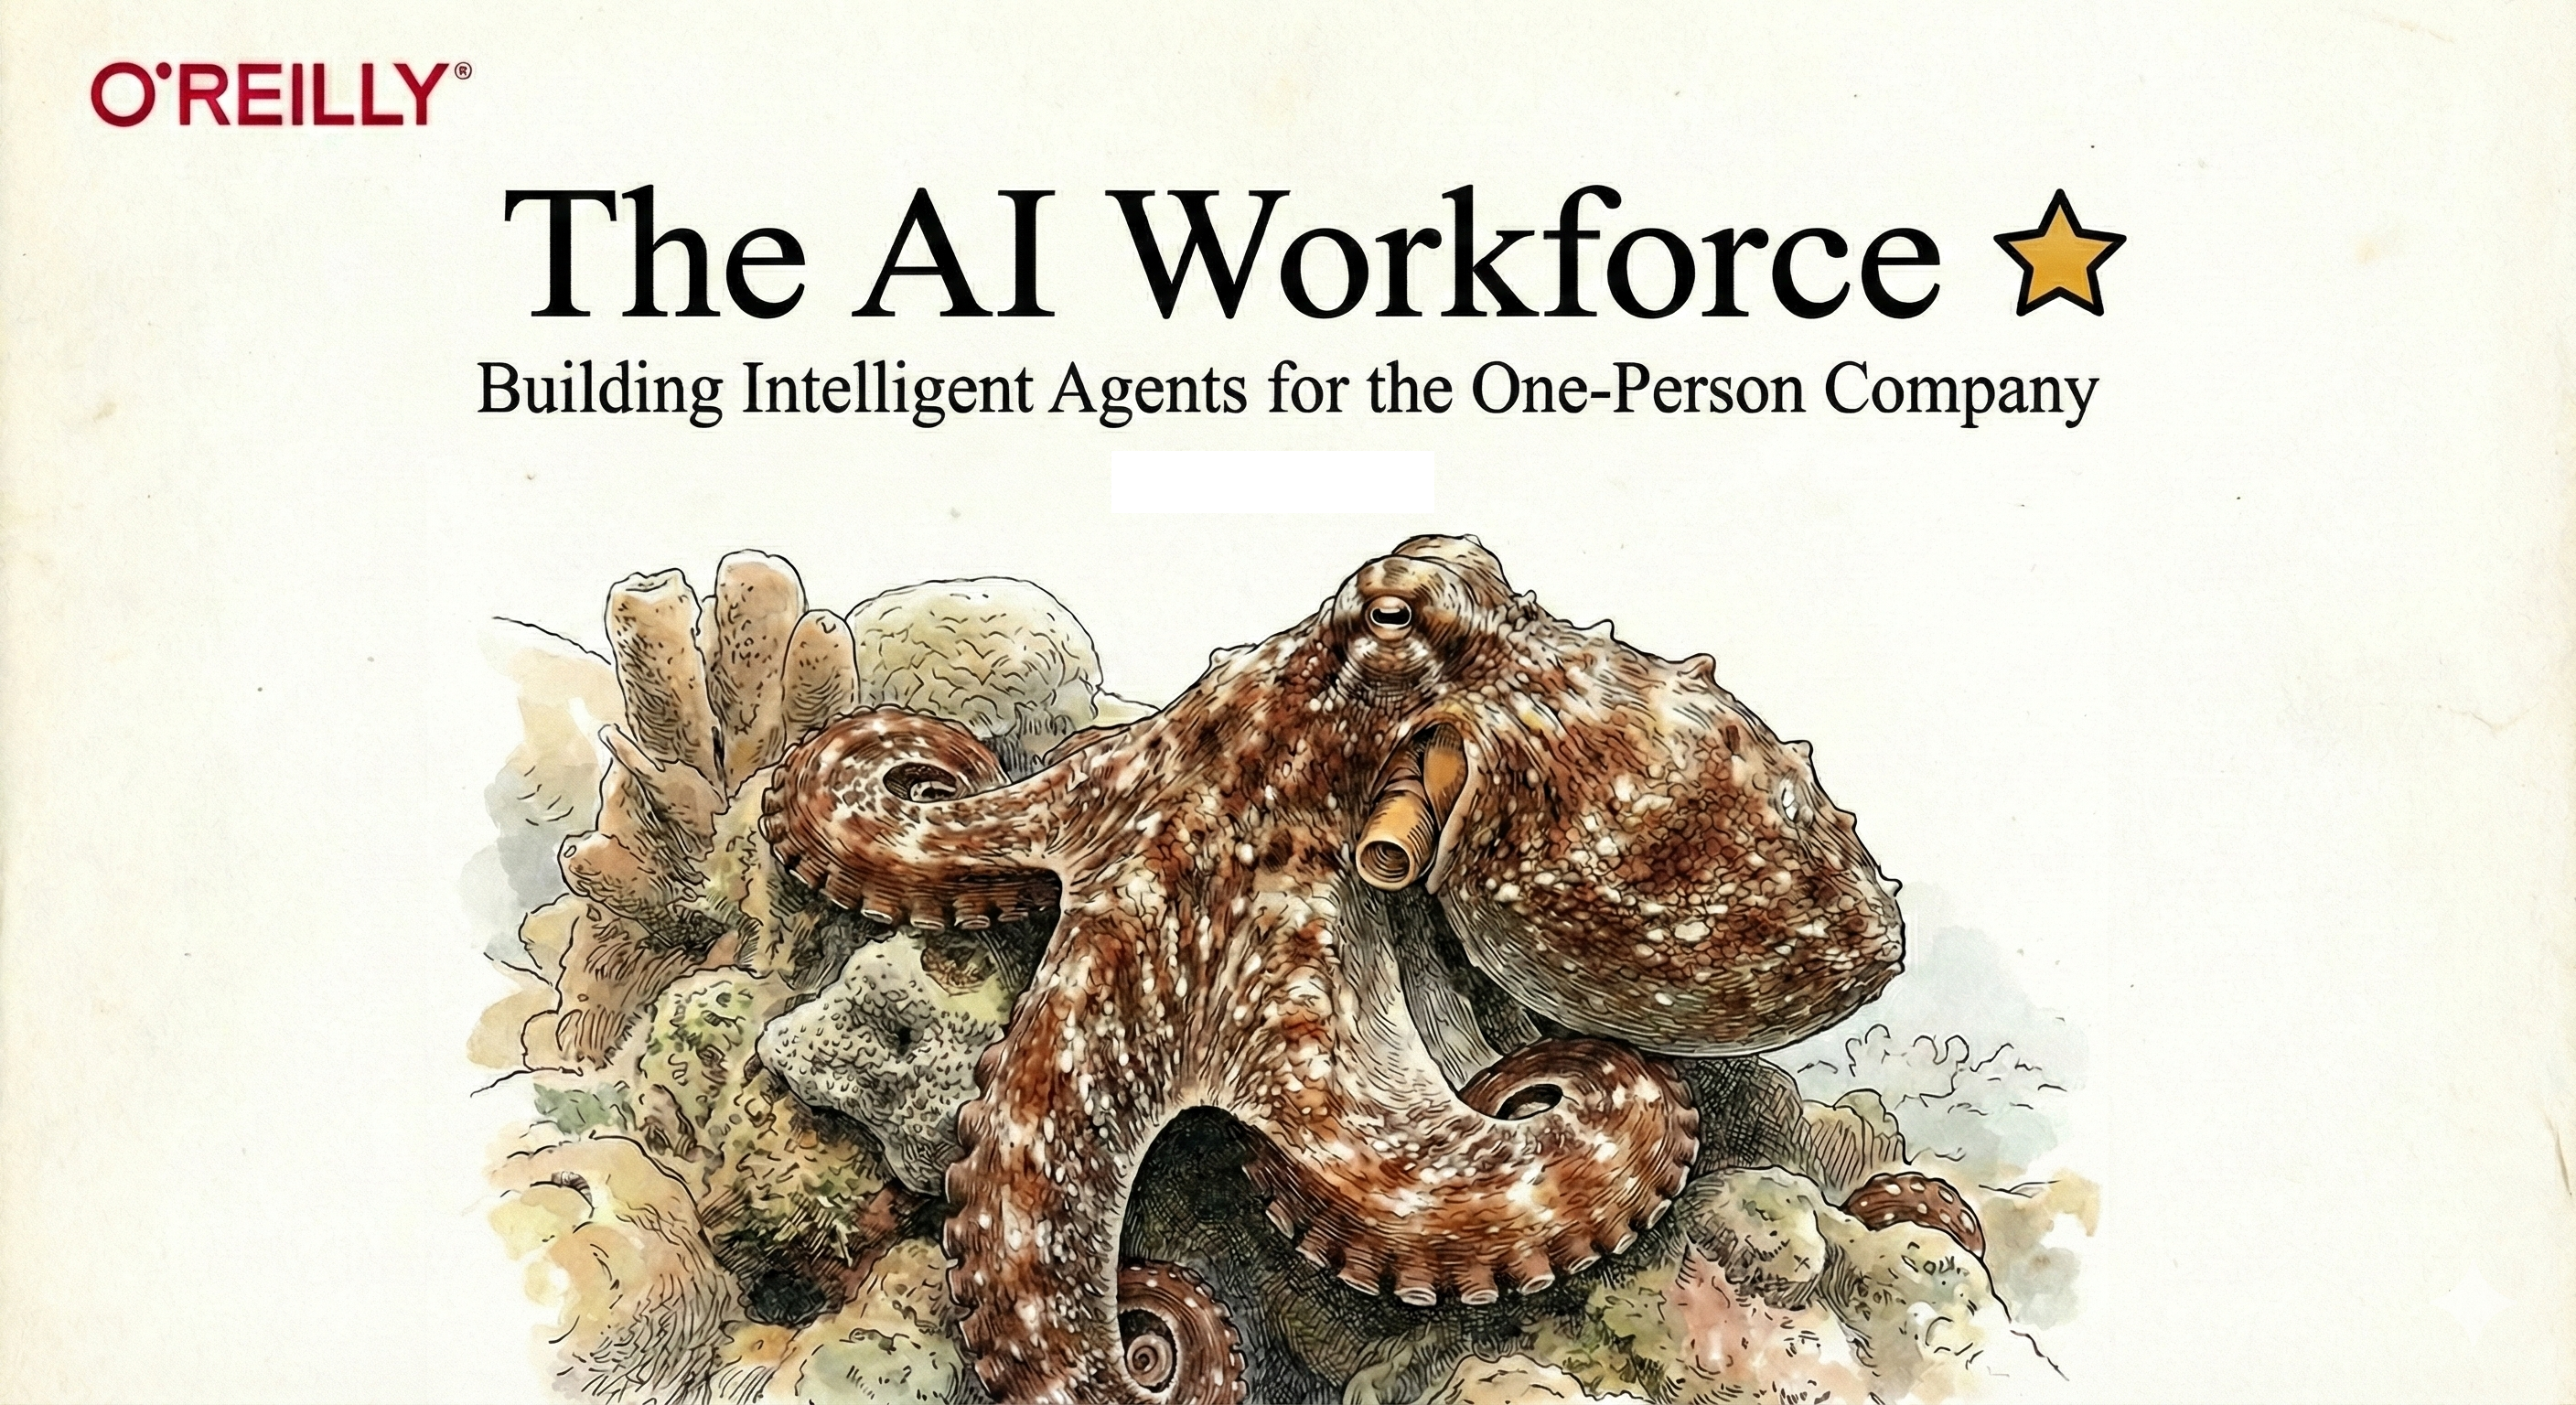
\includegraphics[width=2in]{../images/cover-animal.png}

\vspace{0.5em}

{\large\color{oreilly-red}\textbf{O'REILLY}}

\vspace{0.3em}

{\small oreilly.com}
\end{center}

\end{document}
